
A representação de um genoma por meio de uma sequência de genes é bastante útil e amplamente utilizada em problemas de rearranjo de genomas. Entretanto, informações que não estão associadas diretamente aos genes são descartadas, o que implica em uma perda de informação. Em particular, informações referentes às regiões intergênicas, que são regiões entre cada par consecutivo de genes e nas extremidades de um genoma, não são consideradas pelos modelos que adotam uma representação clássica de um genoma. Estudos sugerem que incorporar tais estruturas aos modelos pode propiciar resultados mais realistas para a distância evolutiva entre os organismos~\cite{2016a-biller-etal, 2016b-biller-etal}. Cada região intergênica possui uma quantidade de nucleotídeos, a qual denominamos de \emph{tamanho} da região intergênica. Neste capítulo, investigaremos as variações com e sem sinais dos seguintes problemas que consideram a informação dos genes e do tamanho das regiões intergênicas de um genoma adotando uma abordagem \emph{não ponderada}:

\begin{itemize}
  \item Ordenação de Permutações por Reversões Intergênicas (\SbIR)
  \item Ordenação de Permutações por Operações Intergênicas de Reversão e Indel (\SbIRI)
  \item Ordenação de Permutações por Operações Intergênicas de Reversão e Move \break (\SbIRM)
  \item Ordenação de Permutações por Operações Intergênicas de Reversão, Move e Indel (\SbIRMI)
  \item Ordenação de Permutações por Operações Intergênicas de Reversão e Transposição (\SbIRT)
  \item Ordenação de Permutações por Operações Intergênicas de Reversão, Transposição e Indel (\SbIRTI)
  \item Ordenação de Permutações por Operações Intergênicas de Reversão, Transposição e Move (\SbIRTM)
  \item Ordenação de Permutações por Operações Intergênicas de Reversão, Transposição, Move e Indel (\SbIRTMI)
\end{itemize}

Além disso, investigaremos as variações com e sem sinais dos seguintes problemas considerando uma abordagem \emph{ponderada}:

\begin{itemize}
  \item Ordenação de Permutações por Operações Intergênicas Ponderadas de Reversão e Indel (\SbWIRI)
  \item Ordenação de Permutações por Operações Intergênicas Ponderadas de Reversão e Transposição (\SbWIRT)
  \item Ordenação de Permutações por Operações Intergênicas Ponderadas de Reversão, Transposição e Indel (\SbWIRTI)
\end{itemize}

Neste capítulo, iremos referenciar aos eventos de rearranjo de reversão intergênica, transposição intergênica, move intergênico e indel intergênico simplesmente por reversão, transposição, move e indel, respectivamente. Além disso, referiremos a um breakpoint intergênico simplesmente por breakpoint. Dada uma sequência de eventos de rearranjo $S$, denotamos por $|S|$ o tamanho da sequência $S$, ou seja, a quantidade de eventos em $S$.

Dada uma instância intergênica rígida com ou sem sinais $\mathcal{I}=((\pi,\breve\pi),(\iota,\breve\iota))$ e adotando um cenário não ponderado, a \emph{distância} entre $(\pi,\breve\pi)$ e $(\iota,\breve\iota)$, denotada por $di_{\mathcal{M}}(\mathcal{I})$, é o tamanho da menor sequência de eventos de rearranjo $S$, tal que todo evento de $S$ pertence ao modelo $\mathcal{M}$ e $(\pi,\breve\pi) \cdot S = (\iota,\breve\iota)$. Os modelos de rearranjo em um cenário não ponderado considerados neste capítulo são identificados pelas siglas apresentadas na Tabela~\ref{table:YQWDTZTK}.

\begin{table}[!htb]
  \caption{Siglas dos modelos de rearranjo considerados para instâncias intergênicas rígidas em um cenário não ponderado.}
  \label{table:YQWDTZTK}
  \centering
  \begin{tabular}{|p{3cm}|p{8cm}|}
    \hline
    \textbf{Sigla}        & \textbf{Conjunto de Eventos de Rearranjo}          \\ \hline
    \SbIR                 & $\{\rho\}                              $           \\ \hline
    \SbIRI                & $\{\rho,\delta\}                       $           \\ \hline
    \SbIRM                & $\{\rho,\mu\}                          $           \\ \hline
    \SbIRMI               & $\{\rho,\mu,\delta\}                   $           \\ \hline
    \SbIRT                & $\{\rho,\tau\}                         $           \\ \hline
    \SbIRTI               & $\{\rho,\tau,\delta\}                  $           \\ \hline
    \SbIRTM               & $\{\rho,\tau,\mu\}                     $           \\ \hline
    \SbIRTMI              & $\{\rho,\tau,\mu,\delta\}              $           \\ \hline
  \end{tabular}
\end{table}

Dada uma instância intergênica rígida com ou sem sinais $\mathcal{I}=((\pi,\breve\pi),(\iota,\breve\iota))$ e adotando um cenário ponderado, a \emph{distância ponderada} entre $(\pi,\breve\pi)$ e $(\iota,\breve\iota)$, denotada por $dwi_{\mathcal{M}}(\mathcal{I})$, é o custo da sequência de eventos de rearranjo $S$ com menor custo total, tal que todo evento de $S$ pertence ao modelo $\mathcal{M}$ e $(\pi,\breve\pi) \cdot S = (\iota,\breve\iota)$. O custo total de uma sequência de eventos de rearranjo $S=(\gamma_1, \gamma_2, \dots, \gamma_k)$, onde cada evento pertence ao modelo $\mathcal{M}$, é dado por $\sum_{\gamma_i \in S} c(\gamma_i)$, tal que $c(\gamma_i)$ representa o custo associado ao tipo do evento $\gamma_i$ por uma função de custo. Os modelos de rearranjo em um cenário ponderado considerados neste capítulo são identificados pelas siglas apresentadas na Tabela~\ref{table:BAORJRQI}.

\begin{table}[!htb]
  \caption{Siglas dos modelos de rearranjo considerados para instâncias intergênicas rígidas em um cenário ponderado.}
  \label{table:BAORJRQI}
  \centering
  \begin{tabular}{|p{2.5cm}|p{3.5cm}|p{8cm}|}
    \hline
    \textbf{Problema}     & \textbf{Sigla do Modelo} & \textbf{Conjunto de Eventos de Rearranjo}          \\ \hline
    \SbWIRI               & \RI                      & $\{\rho,\delta\}                       $           \\ \hline
    \SbWIRT               & \RT                      & $\{\rho,\tau\}                         $           \\ \hline
    \SbWIRTI              & \RTI                     & $\{\rho,\tau,\delta\}                  $           \\ \hline
  \end{tabular}
\end{table}

Quando for adotado um modelo de rearranjo composto exclusivamente por eventos de rearranjo conservativos, será assumido que a instância intergênica rígida para o problema será sempre balanceada.

Parte dos resultados que serão apresentados neste capítulo foram publicados nas revistas \emph{Journal of Computational Biology}~\cite{2020a-brito-etal} e \emph{Algorithms for Molecular Biology}~\cite{2021b-brito-etal} em 2020 e 2021, respectivamente.

% ------------------------------------------------------------------ %
\section{Abordagem não Ponderada}
% ------------------------------------------------------------------ %

Nesta seção, apresentaremos os resultados para as variações com e sem sinais dos problemas \SbIR{}, \SbIRI{}, \SbIRM{}, \SbIRMI{}, \SbIRT{}, \SbIRTI{}, \SbIRTM{} e \SbIRTMI{} em um cenário não ponderado.

% ------------------------------------------------------------------ %
\subsection{Limitantes Inferiores}
% ------------------------------------------------------------------ %

Nesta seção, apresentaremos limitantes inferiores para as variações com e sem sinais dos problemas investigados neste capítulo em um cenário não ponderado.

Em instâncias intergênicas rígidas com e sem sinais utilizaremos os conceitos de breakpoint intergênicos tipo dois e um, respectivamente (Seção~\ref{subsection:JHXBSDPQ}). Os eventos de rearranjo de reversão, transposição, move e indel afetam, respectivamente, as seguintes quantidades de regiões intergênicas: duas, três, duas e uma. No melhor cenário, cada uma das regiões intergênicas afetadas faz parte de um breakpoint removido após o evento de rearranjo ser aplicado. Com isso, obtemos os seguintes lemas.

\begin{lemma}\label{lemma:KFFPUBQG}
Seja $\mathcal{I}$ uma instância intergênica rígida sem sinais. Para qualquer reversão $\rho$ temos que $\Delta ib_1(\mathcal{I}, S = (\rho)) \ge -2$.
\end{lemma}

\begin{lemma}\label{lemma:IUJZCMMV}
Seja $\mathcal{I}$ uma instância intergênica rígida sem sinais. Para qualquer transposição $\tau$ temos que $\Delta ib_1(\mathcal{I}, S = (\tau)) \ge -3$.
\end{lemma}

\begin{lemma}\label{lemma:SYXLGTAP}
Seja $\mathcal{I}$ uma instância intergênica rígida sem sinais. Para qualquer move $\mu$ temos que $\Delta ib_1(\mathcal{I}, S = (\mu)) \ge -2$.
\end{lemma}

\begin{lemma}\label{lemma:KWIVENLG}
Seja $\mathcal{I}$ uma instância intergênica rígida sem sinais. Para qualquer indel $\delta$ temos que $\Delta ib_1(\mathcal{I}, S = (\delta)) \ge -1$.
\end{lemma}

\begin{lemma}\label{lemma:IKBNJWMY}
Seja $\mathcal{I}$ uma instância intergênica rígida com sinais. Para qualquer reversão $\rho$ temos que $\Delta ib_2(\mathcal{I}, S = (\rho)) \ge -2$.
\end{lemma}

\begin{lemma}\label{lemma:MYVALTSG}
Seja $\mathcal{I}$ uma instância intergênica rígida com sinais. Para qualquer transposição $\tau$ temos que $\Delta ib_2(\mathcal{I}, S = (\tau)) \ge -3$.
\end{lemma}

\begin{lemma}\label{lemma:LSPSMYMM}
Seja $\mathcal{I}$ uma instância intergênica rígida com sinais. Para qualquer move $\mu$ temos que $\Delta ib_2(\mathcal{I}, S = (\mu)) \ge -2$.
\end{lemma}

\begin{lemma}\label{lemma:KXIYYHHL}
Seja $\mathcal{I}$ uma instância intergênica rígida com sinais. Para qualquer indel $\delta$ temos que $\Delta ib_2(\mathcal{I}, S = (\delta)) \ge -1$.
\end{lemma}

\begin{theorem}\label{theorem:MPFPKHQO}
Seja $\mathcal{I} = ((\pi,\breve\pi),(\iota,\breve\iota))$ uma instância intergênica rígida sem sinais. Temos que:

\begin{tabular}{lll}
  $di_{\R}(\mathcal{I})$      & $ \ge $ & $\frac{ib_1(\mathcal{I})}{2}$,  \\ 
  $di_{\RI}(\mathcal{I})$     & $ \ge $ & $\frac{ib_1(\mathcal{I})}{2}$,  \\
  $di_{\RM}(\mathcal{I})$     & $ \ge $ & $\frac{ib_1(\mathcal{I})}{2}$,  \\
  $di_{\RMI}(\mathcal{I})$    & $ \ge $ & $\frac{ib_1(\mathcal{I})}{2}$,  \\
  $di_{\RT}(\mathcal{I})$     & $ \ge $ & $\frac{ib_1(\mathcal{I})}{3}$,  \\
  $di_{\RTI}(\mathcal{I})$    & $ \ge $ & $\frac{ib_1(\mathcal{I})}{3}$,  \\
  $di_{\RTM}(\mathcal{I})$    & $ \ge $ & $\frac{ib_1(\mathcal{I})}{3}$ e \\
  $di_{\RTMI}(\mathcal{I})$ & $ \ge $ & $\frac{ib_1(\mathcal{I})}{3}$.    \\
\end{tabular}
\end{theorem}
\begin{proof}
Pela Observação~\ref{remark:UDYJTHAH}, para transformar $(\pi,\breve\pi)$ em $(\iota,\breve\iota)$ é necessário remover os $ib_1(\mathcal{I})$ breakpoints tipo um de $\mathcal{I}$. Dessa forma, obtemos um limitante inferior para cada um dos modelos através da divisão de $ib_1(\mathcal{I})$ pela maior quantidade de breakpoints tipo um que podem ser removidos por um evento permitido no modelo de rearranjo. Os lemas~\ref{lemma:KFFPUBQG}, \ref{lemma:IUJZCMMV}, \ref{lemma:SYXLGTAP} e \ref{lemma:KWIVENLG} mostram a quantidade máxima de breakpoints tipo um que podem ser removidos de uma instância intergênica rígida sem sinais pelos eventos de reversão, transposição, move e indel, respectivamente. Logo, o teorema segue.
\end{proof}

\begin{theorem}\label{theorem:JDOIUJLE}
Seja $\mathcal{I} = ((\pi,\breve\pi),(\iota,\breve\iota))$ uma instância intergênica rígida sem sinais. Se $\mathcal{I}$ for balanceada, então temos que $di_{\RTI}(\mathcal{I}) \ge \frac{ib_1(\mathcal{I})}{3}$. Caso contrário, temos que $di_{\RTI}(\mathcal{I}) \ge \frac{ib_1(\mathcal{I}) + 2}{3}$.
\end{theorem}
\begin{proof}
Pela Observação~\ref{remark:UDYJTHAH}, para transformar $(\pi,\breve\pi)$ em $(\iota,\breve\iota)$ é necessário remover os $ib_1(\mathcal{I})$ breakpoints tipo um de $\mathcal{I}$. Note que se $\mathcal{I}$ for balanceada, então podemos aplicar o Teorema~\ref{theorem:MPFPKHQO}. Caso contrário, sabemos que para ser possível transformar $(\pi,\breve\pi)$ em $(\iota,\breve\iota)$, pelo menos um indel deve ser utilizado. Pelo Lema~\ref{lemma:KWIVENLG}, temos que, no máximo, um breakpoint tipo um pode ser removido utilizando uma operação de indel. No melhor caso, após aplicar apenas um indel, $\mathcal{I}$  torna-se uma instância balanceada e um breakpoint tipo um é removido. Assim, restam $ib_1(\mathcal{I}) - 1$ breakpoints para serem removidos de $\mathcal{I}$. Considerando os eventos de reversão, transposição e indel, três breakpoints tipo um, no máximo, podem ser removidos por operação (lemas~\ref{lemma:KFFPUBQG}, \ref{lemma:IUJZCMMV} e \ref{lemma:KWIVENLG}). Logo, pelo menos $\frac{ib_1(\mathcal{I}) - 1}{3}$ eventos de reversão, transposição ou indel são necessários para remover o restante dos breakpoints tipo um. Dessa forma, pelo menos $\frac{ib_1(\mathcal{I}) - 1}{3} + 1 = \frac{ib_1(\mathcal{I}) + 2}{3}$ eventos de reversão, transposição e indel são necessários para transformar $(\pi,\breve\pi)$ em $(\iota,\breve\iota)$, e o teorema segue.
\end{proof}

\begin{theorem}\label{theorem:NFVKZGKW}
Seja $\mathcal{I} = ((\pi,\breve\pi),(\iota,\breve\iota))$ uma instância intergênica rígida com sinais. Temos que:

\begin{tabular}{lll}
  $di_{\R}(\mathcal{I})$      & $ \ge $ & $\frac{ib_2(\mathcal{I})}{2}$,  \\ 
  $di_{\RI}(\mathcal{I})$     & $ \ge $ & $\frac{ib_2(\mathcal{I})}{2}$,  \\
  $di_{\RM}(\mathcal{I})$     & $ \ge $ & $\frac{ib_2(\mathcal{I})}{2}$,  \\
  $di_{\RMI}(\mathcal{I})$    & $ \ge $ & $\frac{ib_2(\mathcal{I})}{2}$,  \\
  $di_{\RT}(\mathcal{I})$     & $ \ge $ & $\frac{ib_2(\mathcal{I})}{3}$,  \\
  $di_{\RTI}(\mathcal{I})$    & $ \ge $ & $\frac{ib_2(\mathcal{I})}{3}$,  \\
  $di_{\RTM}(\mathcal{I})$    & $ \ge $ & $\frac{ib_2(\mathcal{I})}{3}$ e \\
  $di_{\RTMI}(\mathcal{I})$ & $ \ge $ & $\frac{ib_2(\mathcal{I})}{3}$.    \\
\end{tabular}
\end{theorem}
\begin{proof}
A prova é similar à descrita no Teorema~\ref{theorem:MPFPKHQO}, mas considerando os lemas~\ref{lemma:IKBNJWMY}, \ref{lemma:MYVALTSG}, \ref{lemma:LSPSMYMM} e \ref{lemma:KXIYYHHL}.
\end{proof}

\begin{theorem}\label{theorem:JGVDYLDM}
Seja $\mathcal{I} = ((\pi,\breve\pi),(\iota,\breve\iota))$ uma instância intergênica rígida com sinais. Se $\mathcal{I}$ for balanceada, então temos que $di_{\RTI}(\mathcal{I}) \ge \frac{ib_2(\mathcal{I})}{3}$. Caso contrário, temos que $di_{\RTI}(\mathcal{I}) \ge \frac{ib_2(\mathcal{I}) + 2}{3}$.
\end{theorem}
\begin{proof}
Pela Observação~\ref{remark:UDYJTHAH}, para transformar $(\pi,\breve\pi)$ em $(\iota,\breve\iota)$ é necessário remover os $ib_2(\mathcal{I})$ breakpoints tipo dois de $\mathcal{I}$. Note que se $\mathcal{I}$ for balanceada, então podemos aplicar o Teorema~\ref{theorem:NFVKZGKW}. Caso contrário, sabemos que para ser possível transformar $(\pi,\breve\pi)$ em $(\iota,\breve\iota)$, pelo menos um indel deve ser utilizado. Pelo Lema~\ref{lemma:KXIYYHHL}, temos que, no máximo, um breakpoint tipo dois pode ser removido utilizando uma operação de indel. No melhor caso, após aplicar apenas um indel, $\mathcal{I}$  torna-se uma instância balanceada e um breakpoint tipo dois é removido. Assim, restam $ib_2(\mathcal{I}) - 1$ breakpoints para serem removidos de $\mathcal{I}$. Considerando os eventos de reversão, transposição e indel, três breakpoints tipo um, no máximo, podem ser removidos por operação (lemas~\ref{lemma:IKBNJWMY}, \ref{lemma:MYVALTSG} e \ref{lemma:KXIYYHHL}). Logo, pelo menos $\frac{ib_2(\mathcal{I}) - 1}{3}$ eventos de reversão, transposição ou indel são necessários para remover o restante dos breakpoints tipo dois. Dessa forma, pelo menos $\frac{ib_2(\mathcal{I}) - 1}{3} + 1 = \frac{ib_2(\mathcal{I}) + 2}{3}$ eventos de reversão, transposição e indel são necessários para transformar $(\pi,\breve\pi)$ em $(\iota,\breve\iota)$, e o teorema segue.
\end{proof}

Considerando o grafo de ciclos ponderado rígido (Seção~\ref{subsection:SDWELPAZ}) criado a partir de uma instância intergênica rígida com sinais, o evento de reversão afeta duas arestas pretas do grafo e pode aumentar tanto o número de ciclos como também o número de ciclos balanceados. O evento de transposição afeta três arestas pretas do grafo e pode aumentar tanto o número de ciclos como o número de ciclos balanceados. O evento de move afeta duas arestas pretas do grafo e pode aumentar somente o número de ciclos balanceados no grafo. O evento de indel afeta apenas uma aresta preta do grafo e pode aumentar somente o número de ciclos balanceados. Dessa forma, dada uma instância intergênica rígida com sinais $\mathcal{I} = ((\pi,\breve\pi),(\iota,\breve\iota))$, temos que $\Delta c(G(\mathcal{I}), S=(\rho)) \in \{1,0,-1\}$ e $\Delta c_b(G(\mathcal{I}), S=(\rho)) \in \{1,0,-1\}$ para qualquer reversão $\rho$~\cite{1996-bafna-pevzner,2021b-oliveira-etal}. De maneira similar, temos que $\Delta c(G(\mathcal{I}), S=(\tau)) \in \{2,0,-2\}$ e $\Delta c_b(G(\mathcal{I}), S=(\tau)) \in \{2,1,0,{-1},{-2}\}$ para qualquer transposição $\tau$~\cite{1998-bafna-pevzner,2021a-oliveira-etal}, $\Delta c(G(\mathcal{I}), S=(\mu)) = 0$ e $\Delta c_b(G(\mathcal{I}), S=(\mu)) \in \{2,1,0,{-1},{-2}\}$ para qualquer move $\mu$~\cite{2021a-oliveira-etal}, e $\Delta c(G(\mathcal{I}), S=(\delta)) = 0$ e $\Delta c_b(G(\mathcal{I}), S=(\delta)) \in \{1,0,{-1}\}$ para qualquer indel $\delta$~\cite{2021b-oliveira-etal}. Com isso, obtemos os seguintes limitantes inferiores.

\begin{theorem}\label{theorem:OCNPWYNL}
Seja $\mathcal{I} = ((\pi,\breve\pi),(\iota,\breve\iota))$ uma instância intergênica rígida com sinais. Temos que:

\begin{tabular}{lll}
  $di_{\RM}(\mathcal{I})$       & $ \ge $ & ${n + 1} - \frac{c(G(\mathcal{I})) + c_b(G(\mathcal{I}))}{2}$ e \\
  $di_{\RMI}(\mathcal{I})$    & $ \ge $ & ${n + 1} - \frac{c(G(\mathcal{I})) + c_b(G(\mathcal{I}))}{2}$.    \\
\end{tabular}
\end{theorem}
\begin{proof}
Note que, para atingir o genoma alvo, é necessário aumentar tanto o número de ciclos quanto o de ciclos balanceados em $G(\mathcal{I})$ para $n+1$ (Observação~\ref{remark:WVLFPRDL}). Dados os eventos de reversão, move e indel, temos que $c(G(\mathcal{I})) + c_b(G(\mathcal{I}))$ pode aumentar, no máximo, em duas unidades. Logo, o teorema segue.
\end{proof}

\begin{theorem}\label{theorem:ZZBNVROM}
Seja $\mathcal{I} = ((\pi,\breve\pi),(\iota,\breve\iota))$ uma instância intergênica rígida com sinais. Temos que:

\begin{tabular}{lll}
  $di_{\RTI}(\mathcal{I})$       & $ \ge $ & $\frac{{n + 1} - c_b(G(\mathcal{I}))}{2}$ e \\
  $di_{\RTMI}(\mathcal{I})$    & $ \ge $ & $\frac{{n + 1} - c_b(G(\mathcal{I}))}{2}$.    \\
\end{tabular}
\end{theorem}
\begin{proof}
Note que, para atingir o genoma alvo, é necessário aumentar o número de ciclos balanceados em $G(\mathcal{I})$ para $n+1$ (Observação~\ref{remark:WVLFPRDL}). Dados os eventos de reversão, transposição, move e indel, temos que $c_b(G(\mathcal{I}))$ pode aumentar, no máximo, em duas unidades. Logo, o teorema segue.
\end{proof}

% ------------------------------------------------------------------ %
\subsection{Análise de Complexidade}
% ------------------------------------------------------------------ %

Nesta seção, realizaremos uma análise de complexidade considerando as variações com e sem sinais dos problemas investigados neste capítulo em um cenário não ponderado. Os problemas citados e investigados nessa seção referem-se a suas respectivas versões de decisão.

Inicialmente, descrevemos a versão de decisão de alguns problemas, sendo eles:
\begin{itemize}
  \item A variação sem sinais do problema de Ordenação de Permutações por Reversões (\SbR)
  \item As variações com e sem sinais do problema de Ordenação de Permutações por Reversões e Transposições (\SbRT)
  \item O problema $3$-Partição (\textbf{3-PART}).
\end{itemize}
Esses três problemas pertencem à classe NP-difícil~\cite{1999a-caprara,2019b-oliveira-etal,1990-garey-johnson}.

\begin{decision}
  \problemtitle{(\SbR) (Versão de Decisão)}
  \probleminput{Uma instância clássica sem sinais $\mathcal{I}=(\pi,\iota)$ e um número natural $d$.}
  \problemquestion{Existe uma sequência de eventos de rearranjo $S$, com base no modelo de rearranjo $\mathcal{M}=\{\rho\}$, capaz de transformar $\pi$ em $\iota$, tal que $|S| \le d$?}
\end{decision}

\begin{decision}
  \problemtitle{(\SbRT) (Versão de Decisão)}
  \probleminput{Uma instância clássica com ou sem sinais $\mathcal{I}=(\pi,\iota)$ e um número natural $d$.}
  \problemquestion{Existe uma sequência de eventos de rearranjo $S$, com base no modelo de rearranjo $\mathcal{M}=\{\rho,\tau\}$, capaz de transformar $\pi$ em $\iota$, tal que $|S| \le d$?}
\end{decision}

\begin{decision}
  \problemtitle{(\textbf{3-PART}) (Versão de Decisão)}
  \probleminput{Um conjunto de números inteiros positivos $A=\{a_1,a_2,\dots,a_{3n}\}$, tal que $\sum_{i=1}^{3n}a_i = Bn$ e $B \in \mathbb{Z}^{+}$. Além disso, $\frac{B}{4} < a_i < \frac{B}{2}$, com $1 \le i \le 3n$.}
  \problemquestion{Existe uma partição do conjunto $A$ em triplas $A_1,A_2,\dots,A_n$, tal que $\sum_{a_i \in A_j} a_i = B$ para cada tripla $A_j$, com $1\le j \le n$?}
\end{decision}

A seguir, descrevemos a versão de decisão das variações com e sem sinais dos problemas que investigaremos neste capítulo em um cenário não ponderado.

\begin{decision}
  \problemtitle{\SbIR{} (Versão de Decisão)}
  \probleminput{Um número natural $t$ e uma instância intergênica rígida com ou sem sinais $\mathcal{I}=((\pi,\breve\pi),(\iota,\breve\iota))$.}
  \problemquestion{Existe uma sequência de eventos de rearranjo $S$, com base no modelo de rearranjo $\mathcal{M}=\{\rho\}$, capaz de transformar $(\pi,\breve\pi)$ em $(\iota,\breve\iota)$, tal que $|S| \le t$?}
\end{decision}

\begin{decision}
  \problemtitle{\SbIRI{} (Versão de Decisão)}
  \probleminput{Um número natural $t$ e uma instância intergênica rígida com ou sem sinais $\mathcal{I}=((\pi,\breve\pi),(\iota,\breve\iota))$.}
  \problemquestion{Existe uma sequência de eventos de rearranjo $S$, com base no modelo de rearranjo $\mathcal{M}=\{\rho,\delta\}$, capaz de transformar $(\pi,\breve\pi)$ em $(\iota,\breve\iota)$, tal que $|S| \le t$?}
\end{decision}

\begin{decision}
  \problemtitle{\SbIRM{} (Versão de Decisão)}
  \probleminput{Um número natural $t$ e uma instância intergênica rígida com ou sem sinais $\mathcal{I}=((\pi,\breve\pi),(\iota,\breve\iota))$.}
  \problemquestion{Existe uma sequência de eventos de rearranjo $S$, com base no modelo de rearranjo $\mathcal{M}=\{\rho,\mu\}$, capaz de transformar $(\pi,\breve\pi)$ em $(\iota,\breve\iota)$, tal que $|S| \le t$?}
\end{decision}

\begin{decision}
  \problemtitle{\SbIRMI{} (Versão de Decisão)}
  \probleminput{Um número natural $t$ e uma instância intergênica rígida com ou sem sinais $\mathcal{I}=((\pi,\breve\pi),(\iota,\breve\iota))$.}
  \problemquestion{Existe uma sequência de eventos de rearranjo $S$, com base no modelo de rearranjo $\mathcal{M}=\{\rho,\mu,\delta\}$, capaz de transformar $(\pi,\breve\pi)$ em $(\iota,\breve\iota)$, tal que $|S| \le t$?}
\end{decision}

\begin{decision}
  \problemtitle{\SbIRT{} (Versão de Decisão)}
  \probleminput{Um número natural $t$ e uma instância intergênica rígida com ou sem sinais $\mathcal{I}=((\pi,\breve\pi),(\iota,\breve\iota))$.}
  \problemquestion{Existe uma sequência de eventos de rearranjo $S$, com base no modelo de rearranjo $\mathcal{M}=\{\rho,\tau\}$, capaz de transformar $(\pi,\breve\pi)$ em $(\iota,\breve\iota)$, tal que $|S| \le t$?}
\end{decision}

\begin{decision}
  \problemtitle{\SbIRTI{} (Versão de Decisão)}
  \probleminput{Um número natural $t$ e uma instância intergênica rígida com ou sem sinais $\mathcal{I}=((\pi,\breve\pi),(\iota,\breve\iota))$.}
  \problemquestion{Existe uma sequência de eventos de rearranjo $S$, com base no modelo de rearranjo $\mathcal{M}=\{\rho,\tau,\delta\}$, capaz de transformar $(\pi,\breve\pi)$ em $(\iota,\breve\iota)$, tal que $|S| \le t$?}
\end{decision}

\begin{decision}
  \problemtitle{\SbIRTM{} (Versão de Decisão)}
  \probleminput{Um número natural $t$ e uma instância intergênica rígida com ou sem sinais $\mathcal{I}=((\pi,\breve\pi),(\iota,\breve\iota))$.}
  \problemquestion{Existe uma sequência de eventos de rearranjo $S$, com base no modelo de rearranjo $\mathcal{M}=\{\rho,\tau,\mu\}$, capaz de transformar $(\pi,\breve\pi)$ em $(\iota,\breve\iota)$, tal que $|S| \le t$?}
\end{decision}

\begin{decision}
  \problemtitle{\SbIRTMI{} (Versão de Decisão)}
  \probleminput{Um número natural $t$ e uma instância intergênica rígida com ou sem sinais $\mathcal{I}=((\pi,\breve\pi),(\iota,\breve\iota))$.}
  \problemquestion{Existe uma sequência de eventos de rearranjo $S$, com base no modelo de rearranjo $\mathcal{M}=\{\rho,\tau,\mu,\delta\}$, capaz de transformar $(\pi,\breve\pi)$ em $(\iota,\breve\iota)$, tal que $|S| \le t$?}
\end{decision}

A seguir mostramos que todas as variações sem sinais dos problemas investigados nesse capítulo, em um cenário não ponderado, pertencem à classe NP-difícil.

\begin{theorem}\label{theorem:YARJETHG}
Os problemas \SbIR{}, \SbIRI{}, \SbIRM{} e \SbIRMI{} em instâncias intergênicas rígidas sem sinais pertencem à classe NP-difícil.
\end{theorem}
\begin{proof}
Dada uma instância clássica sem sinais $\mathcal{I}=(\pi,\iota)$ e um valor $d$ para a versão de decisão do problema \SbR, criaremos uma instância intergênica rígida sem sinais $\mathcal{I'}=((\pi',\breve\pi'),(\iota',\breve\iota'))$ e um valor $t$ para a versão de decisão do problema \SbIR{}, \SbIRI{}, \SbIRM{} ou \SbIRMI{} da seguinte maneira: (i) $\pi' = \pi$, (ii) $\iota' = \iota$, (iii) $\breve\pi' = \breve\iota' = (0,0,\dots,0)$ e (iv) $t = d$. Agora mostramos que a instância $(\mathcal{I},d)$ do problema \SbR{} é sim se, e somente se, a instância $(\mathcal{I'},t)$ do problema \SbIR{}, \SbIRI{}, \SbIRM{} ou \SbIRMI{} é sim.

($\Rightarrow$) Suponha que exista uma sequência $S$ com $d$ reversões, tal que $\pi \cdot S = \iota$. Considere a sequência $S'$ criada a partir da sequência $S$ mapeando cada reversão $\rho^{(i,j)}$ em uma reversão intergênica $\rho^{(i,j)}_{(0,0)}$. Note que $(\pi,\breve\pi) \cdot S' = (\iota,\breve\iota)$ e $|S'| = t = d$, uma vez que o tamanho de todas as regiões intergênicas no genoma de origem e alvo é zero.

($\Leftarrow$) Agora suponha que exista uma sequência $S'$ com $t$ eventos de rearranjo tal que $(\pi,\breve\pi) \cdot S' = (\iota,\breve\iota)$. Primeiramente, mostraremos que se a sequência $S'$ não for composta exclusivamente por reversões intergênicas, então ela pode ser modificada para possuir tal característica mantendo a resposta positiva para a instância $(\mathcal{I'},t)$. Seja $S'$ uma sequência que gera uma resposta positiva para a instância $(\mathcal{I'},t)$ do problema \SbIR{}, \SbIRI{}, \SbIRM{} ou \SbIRMI{} e não é composta exclusivamente por reversões intergênicas. Neste caso, criaremos uma sequência $S''$ composta exclusivamente por reversões intergênicas, tal que  $|S''| < |S'|$ e $(\pi,\breve\pi) \cdot S'' = (\iota,\breve\iota)$. Para cada reversão intergênica $\rho^{(i,j)}_{(x,y)}$ de $S'$ adicione em $S''$ a reversão intergênica $\rho^{(i,j)}_{(0,0)}$. Note que os eventos de move e indel não afetam a ordem dos genes. Além disso, pela construção de $\mathcal{I'}$, temos que $\breve\pi' = \breve\iota'$. Logo, $(\pi,\breve\pi) \cdot S'' = (\iota,\breve\iota)$. Por fim, substitua $S'$ por $S''$. Agora, com $S'$ composta exclusivamente por reversões intergênicas, considere a sequência $S$ criada a partir da sequência $S'$ mapeando cada reversão intergênica $\rho^{(i,j)}_{(x,y)}$ em uma reversão $\rho^{(i,j)}$. É importante notar que, como a sequência $S'$ é composta exclusivamente por reversões intergênicas, isso implica que nenhum nucleotídeo é inserido no genoma de origem. Logo, para cada reversão intergênica $\rho^{(i,j)}_{(x,y)}$ de $S'$, temos que $x=y=0$ e isso faz com que seja possível realizar tal mapeamento. Dessa forma, temos que $\pi \cdot S = \iota$ e $|S| \le t = d $. Logo, o teorema segue.
\end{proof}

\begin{theorem}\label{theorem:RDOZOOIB}
Os problemas \SbIRT, \SbIRTI, \SbIRTM{} e \SbIRTMI{} em instâncias intergênicas rígidas sem sinais pertencem à classe NP-difícil.
\end{theorem}
\begin{proof}
A prova é similar à descrita no Teorema~\ref{theorem:YARJETHG}, mas utilizando uma redução da versão de decisão da variação sem sinais do problema \SbRT{} e considerando que a sequência $S'$ para a instância $(\mathcal{I'},t)$ do problema \SbIRT{}, \SbIRTI{}, \SbIRTM{} ou \SbIRTMI{} é composta por reversões intergênicas e transposições intergênicas ao invés de ser composta exclusivamente por reversões intergênicas.
\end{proof}

Os problemas \SbIR{}, \SbIRT{} e \SbIRTM{} em instâncias intergênicas rígidas com sinais pertencem à classe NP-difícil~\cite{2021a-oliveira-etal,2021b-oliveira-etal}. A seguir, mostramos que a variação com sinais dos problemas \SbIRM{}, \SbIRMI{}, \SbIRTI{} e \SbIRTMI{} também pertencem à classe NP-difícil. Para a variação com sinais dos problemas \SbIRM{} e \SbIRMI{} iremos realizar uma redução do problema \textbf{3-PART}, enquanto que para a variação com sinais dos problemas \SbIRTI{} e \SbIRTMI{} utilizaremos um redução da variação com sinais do problema \SbRT{}.

\begin{theorem}\label{theorem:FETVDCDT}
Os problemas \SbIRM{} e \SbIRMI{} em instâncias intergênicas rígidas com sinais pertencem à classe NP-difícil.
\end{theorem}
\begin{proof}
Dada uma instância $A=\{a_1,a_2,\dots,a_{3n}\}$ do problema \textbf{3-PART}, criamos uma instância intergênica rígida com sinais $\mathcal{I} = ((\pi,\breve\pi ),(\iota,\breve\iota))$ do problema \SbIRM{} ou \SbIRMI{} da seguinte forma:
\begin{itemize}
    \item[i.] $\pi = \iota = ({+0}~{+1}~{+2}~\dots~{+4n})$.
    \item[ii.] Atribua o valor $\breve\pi_i = a_i$, para $1 \le i \le 3n$, e o valor $\breve\pi_j = 0$, para $3n+1 \le j \le 4n$.
    \item[iii.] Atribua o valor $\breve\iota_i = 0$, para $1 \le i \le 3n$, e o valor $\breve\iota_j = B$, para $3n+1 \le j \le 4n$.
    \item[iv.] $t = 3n.$
\end{itemize}

O Exemplo~\ref{example:ZVSSIKRT} ilustra o processo de criação de uma instância $\mathcal{I}$ do problema \SbIRM{} ou \SbIRMI{} com base na instância $A$ do problema \textbf{3-PART}. Note que o grafo de ciclos ponderado rígido $G(\mathcal{I})$ é composto exclusivamente por ciclos triviais.

\pagebreak
\begin{example}\label{example:ZVSSIKRT}
    \hfill \break
    \begin{center}
    \resizebox{.95\textwidth}{!}{
        \begin{tikzpicture}[arrow/.style={single arrow,
        draw=black,
        fill=#1,
        single arrow head extend=2mm
        }]
        \node[draw=none,fill=none, minimum height=1cm, minimum width=6cm, align=center] at (9.75, 1.0) {$A=\{a_1,a_2,\dots,a_{3n}\}$};
        
        %%%% (arrow)
        \node[arrow, rotate=270, draw=black, fill=white, minimum size=8mm](arrow) at (9.75,0.10) {};
    
        %%%%% (pi)
        \node[draw=none, fill=none, minimum height=1cm, minimum width=12cm, text ragged, text width=12cm] at (9.75, -1.0) {$(\pi,\breve\pi)~=~(({+0}~{+1}~{+2}~\dots~{+4n}),(a_1,a_2,\dots,a_{3n},\:\:0,\:0,\dots,\:0))$};
        
        %%%%% (iota)
        \node[draw=none, fill=none, minimum height=1cm, minimum width=12cm, text ragged, text width=12cm] at (9.75, -1.75) {$(\iota,\breve\iota)~~~=~(({+0}~{+1}~{+2}~\dots~{+4n}),(\:\:0,\:\:0,\dots,\:\:\:\:0,\:B,B,\dots,B))$};
        
        %%%%% (I)
        \node[draw=none,fill=none, minimum height=1cm, minimum width=12cm, text ragged, text width=12cm] at (9.75, -2.50) {$\mathcal{I} = ((\pi,\breve\pi),(\iota,\breve\iota))$};
        
        %%%% (arrow)
        \node[arrow, rotate=270, draw=black, fill=white, minimum size=8mm](arrow) at (9.75,-3.0) {};
        
        %%%% G(I)
        \node[draw=none,fill=none] at (9.75, -4.25) {$G(\mathcal{I})$};
        
        \draw (-0.5,-7.0) -- (9.5,-7.0) ;
        \draw (-0.5,-6.75) -- (-0.5,-7.25) ;
        \draw (9.5,-6.75) -- (9.5,-7.25) ;
        \node[draw=none,fill=none] at (4.5, -7.35) {$3n$ ciclos triviais negativos};
        
        \draw (10.0,-7.0) -- (20.0,-7.0) ;
        \draw (10.0,-6.75) -- (10.0,-7.25) ;
        \draw (20.0,-6.75) -- (20.0,-7.25) ;
        \node[draw=none,fill=none] at (15.0, -7.35) {$n$ ciclos triviais positivos};
        
        
        \begin{scope}[every node/.style={inner sep=1.5pt, minimum size = 0pt}]
            \node[circle, draw, minimum size=0.5cm] (p0) at (0.0,-6.0) {$+0$};
            \node[circle, draw, minimum size=0.5cm] (m1) at (1.5,-6.0) {$-1$};
            \node[circle, draw, minimum size=0.5cm] (p1) at (3.0,-6.0) {$+1$};
            \node[circle, draw, minimum size=0.5cm] (m2) at (4.5,-6.0) {$-2$};
            \node[circle, draw=none, fill=none, minimum size=0.75cm] (dots) at (6.0,-6.0) {$\dots$};
            \node[circle, draw, minimum size=0.5cm] (pn) at (7.5,-6.0) {};
            \node[circle, draw, minimum size=0.5cm] (mn1) at (9.0,-6.0) {};
            \node[circle, draw, minimum size=0.5cm] (pn1) at (10.5,-6.0) {};
            \node[circle, draw, minimum size=0.5cm] (mn2) at (12.0,-6.0) {};
            \node[circle, draw, minimum size=0.5cm] (pn2) at (13.5,-6.0) {};
            \node[circle, draw, minimum size=0.5cm] (mn3) at (15.0,-6.0) {};
            \node[circle, draw=none, fill=none, minimum size=0.5cm] (dots) at (16.5,-6.0) {$\dots$};
            \node[circle, draw, minimum size=0.5cm] (p4n) at (18.0,-6.0) {};
            \node[circle, draw, minimum size=0.5cm] (m4n1) at (19.5,-6.0) {};
        
        \end{scope}
        
        \begin{scope}[>={Stealth[black]},
                      every edge/.style={draw=black}]
            \path [-] (p0) edge node [black, pos=0.5, sloped, above] {$a_1$} node [black, pos=0.5, sloped, below, yshift=-0.15cm] {$1$} (m1);
            \path [-] (p1) edge node [black, pos=0.5, sloped, above] {$a_2$} node [black, pos=0.5, sloped, below, yshift=-0.15cm] {$2$} (m2);
            \path [-] (pn) edge node [black, pos=0.5, sloped, above] {$a_{3n}$} node [black, pos=0.5, sloped, below, yshift=-0.15cm] {$3n$} (mn1);
            \path [-] (pn1) edge node [black, pos=0.5, sloped, above] {$0$} node [black, pos=0.5, sloped, below, yshift=-0.15cm] {$3n{+1}$} (mn2);
            \path [-] (pn2) edge node [black, pos=0.5, sloped, above] {$0$} node [black, pos=0.5, sloped, below, yshift=-0.15cm] {$3n{+2}$} (mn3);
            \path [-] (p4n) edge node [black, pos=0.5, sloped, above] {$0$} node [black, pos=0.5, sloped, below, yshift=-0.15cm] {$4n$} (m4n1);
        \end{scope}
        
        \begin{scope}[>={Stealth[black]},
                      every edge/.style={draw=black}]
            \path [-] (p0) edge [bend left=70, dashed] node [black, pos=0.5, sloped, above] {$0$} (m1);
            \path [-] (p1) edge [bend left=70, dashed] node [black, pos=0.5, sloped, above] {$0$} (m2);
            \path [-] (pn) edge [bend left=70, dashed] node [black, pos=0.5, sloped, above] {$0$} (mn1);
            \path [-] (pn1) edge [bend left=70, dashed] node [black, pos=0.5, sloped, above] {$B$} (mn2);
            \path [-] (pn2) edge [bend left=70, dashed] node [black, pos=0.5, sloped, above] {$B$} (mn3);
            \path [-] (p4n) edge [bend left=70, dashed] node [black, pos=0.5, sloped, above] {$B$} (m4n1);
        \end{scope}
    \end{tikzpicture}
    }
    \end{center}
    \hfill
\end{example}

Agora, mostramos que a instância $A$ do \textbf{3-PART} é sim se, e somente se, \break$di_{\RM}(\mathcal{I}) \le t = 3n$ e $di_{\RMI}(\mathcal{I}) \le t = 3n$.

($\Rightarrow$) Suponha que seja possível particionar a instância $A=\{a_1,a_2,\dots,a_{3n}\}$ do problema \textbf{3-PART} em $n$ triplas, tal que $\sum_{a_i \in A_j} a_i = B$ para cada tripla $A_j$, com $1\le j \le n$. Então, é possível transformar o genoma de origem $(\pi, \breve\pi)$ no genoma alvo $(\iota, \breve\iota)$ usando $3n$ operações de move. Para cada tripla $A_j$, com $1\le j \le n$, aplique as seguintes operações de move $\mu_{(a_i)}^{(i,3n+j)}$, para $a_i \in A_j$. Repita esse procedimento em todas as $n$ triplas, produzindo uma sequência de $3n$ operações de move que resulta em $c(G(\mathcal{I})) = c_b(G(\mathcal{I})) = 4n$. Assim, $di_{\RM}(\mathcal{I}) \le 3n$ e $di_{\RMI}(\mathcal{I}) \le 3n$.

($\Leftarrow$) Agora suponha que $di_{\RM}(\mathcal{I}) \le 3n$ e $di_{\RMI}(\mathcal{I}) \le 3n$. Observe que, para atingir o genoma alvo desejado, os ciclos triviais com arestas pretas rotuladas com o valor $0$ até $3n$ devem formar ciclos triviais com peso zero em suas arestas pretas.

Note que $G(\mathcal{I})$ tem $4n$ ciclos triviais, onde: os primeiros $3n$ ciclos triviais (da esquerda para a direita usando a representação padrão de $G(\mathcal{I})$) têm peso positivo em suas arestas pretas; e os últimos $n$ ciclos triviais têm peso zero em suas arestas pretas.

Dizemos que um ciclo $C=(c^1)$ é \emph{alpha} se $C$ for trivial e tiver peso zero em suas duas arestas (preta e cinza). Denotamos por $c_{\alpha}(G(\mathcal{I}))$ o número de ciclos alpha em $G(\mathcal{I})$. Observe que qualquer sequência de operações de rearranjo que transforme o genoma de origem no genoma alvo deve, necessariamente, afetar os primeiros $3n$ ciclos triviais para alterar o peso em suas arestas pretas para zero. Consequentemente, ao alcançar o genoma alvo temos que $c_{\alpha}(G(\mathcal{I})) = 3n$.

Dada uma sequência $S$ de operações, denotamos por: $$\Delta c_{\alpha}(G(\mathcal{I}), S) = \frac{c_{\alpha}(G(\mathcal{I'})) - c_{\alpha}(G(\mathcal{I}))}{|S|},$$ tal que $\mathcal{I'} = ((\pi,\breve\pi) \cdot S,(\iota,\breve\iota))$, a variação média no número de ciclos alpha gerados pela sequência $S$.

Um move $\mu_{(x)}^{(i,j)}$ atua em até dois ciclos. Se o move $\mu$ atua em duas arestas pretas do mesmo ciclo, então o peso desse ciclo permanece inalterado ($\Delta c_{\alpha}(G(\mathcal{I}), S=(\mu)) = 0$). Quando atua em dois ciclos, temos os seguintes casos:
\begin{itemize}
  \item Se nenhum dos ciclos for trivial, então $\Delta c_{\alpha}(G(\mathcal{I}), S=(\mu)) = 0$, dado que a operação de move não altera o tamanho dos ciclos.
  \item Se pelo menos um dos ciclos for trivial, então o move pode transferir o peso em sua aresta preta para outro ciclo e, na melhor das hipóteses, $\Delta c_{\alpha}(G(\mathcal{I}), S=(\mu)) \le 1$.
  \item Se ambos os ciclos são alpha, então $\Delta c_{\alpha}(G(\mathcal{I}), S=(\mu)) = 0$, dado que, neste caso, as arestas pretas de ambos os ciclos têm peso zero. Consequentemente, o peso da aresta preta dos ciclos permanece inalterado.
\end{itemize}

Uma reversão $\rho_{(x,y)}^{(i,j)}$ pode criar até dois ciclos alpha ($\Delta c_{\alpha}(G(\mathcal{I}), S=(\rho)) \le 2$). No entanto, isso ocorre apenas no caso particular em que uma reversão divide um ciclo de tamanho dois onde ambas as arestas pretas têm peso zero. Dado que uma operação de move não altera o tamanho dos ciclos, para obter um ciclo de tamanho dois com tal característica, temos que uma reversão $\rho$ que une dois ciclos deve ser aplicada previamente. Observe que qualquer reversão que une ciclos não cria ciclos alpha ($\Delta c_{\alpha}(G(\mathcal{I}), S=(\rho)) \le 0$), pois esta operação resulta em um ciclo não trivial. Para obter um ciclo de tamanho dois onde ambas as arestas pretas tenham peso zero, temos três possibilidades:

\begin{itemize}
  \item O primeiro caso consiste em uma reversão $\rho_1$, que une dois ciclos alpha (diminuindo o número de ciclos alpha em duas unidades), seguida por uma reversão $\rho_2$, que divide esse ciclo de tamanho dois gerado em dois ciclos alpha novamente. Observe que neste caso a reversão $\rho_2$ desfaz $\rho_1$, então $\Delta c_{\alpha}(G(\mathcal{I}), S=(\rho_1,\rho_2)) = 0 $, uma vez que $\Delta c_{\alpha}(G(\mathcal{I}), S=(\rho_1)) = -2$ e $\Delta c_{\alpha}(G(\mathcal{I}), S=(\rho_2)) = 2$.
  \item No segundo caso, temos uma reversão $\rho_1$ que une dois ciclos triviais onde ambas as arestas pretas têm peso maior que zero. Pela construção do ciclo de tamanho dois, temos que pelo menos uma de suas arestas pretas tem peso maior que zero. Para remover o peso nas arestas pretas do ciclo de tamanho dois, pelo menos um move $\mu_1$ deve ser aplicado. Observe que o move $\mu_1$ não cria ciclos alpha ($\Delta c_{\alpha}(G(\mathcal{I}), s=(\mu_1)) \le 0$), pois transfere o peso de uma aresta preta de um ciclo de tamanho dois para outro ciclo. Por fim, é aplicada uma reversão $\rho_2$, que divide o ciclo de tamanho dois, gerando dois ciclos alpha. Observe que $\Delta c_{\alpha}(G(\mathcal{I}), S=(\rho_1,\mu_1,\rho_2)) \le \frac{2}{3}$, uma vez que $\Delta c_{ \alpha}(G(\mathcal{I}), S=(\rho_1)) = 0$, $\Delta c_{\alpha}(G(\mathcal{I}), S=(\mu_1)) \le 0$ e $\Delta c_{\alpha}(G(\mathcal{I}), S=(\rho_2)) = 2$.
  \item A última possibilidade é quando uma reversão $\rho_1$ une um ciclo trivial cuja aresta preta tem peso maior que zero com um ciclo alpha, diminuindo o número de ciclos alpha em uma unidade. Semelhante ao caso anterior, pelo menos uma das arestas pretas no ciclo de tamanho dois tem peso maior que zero e, pelo menos uma operação de move $\mu_1$ deve ser aplicada. No final, uma reversão $\rho_2$ é aplicada no ciclo de tamanho dois, gerando dois ciclos alpha. Esse caso resulta em $\Delta c_{\alpha}(G(\mathcal{I}), S=(\rho_1,\mu_1,\rho_2)) \le \frac{1}{3}$, uma vez que $\Delta c_{\alpha}(G(\mathcal{I}), S=(\rho_1)) = -1$, $\Delta c_{\alpha}(G(\mathcal{I}), S=(\mu_1)) \le 0$ e $\Delta c_{\alpha}(G(\mathcal{I}), S=(\rho_2)) = 2$.
\end{itemize}

Considerando o cenário em que uma reversão cria apenas um ciclo alpha, também temos o fato de que uma reversão que une ciclos deve ser aplicada previamente. Assim, temos que $\Delta c_{\alpha}(G(\mathcal{I}), S=(\rho_1,\rho_2)) \le \frac{1}{2}$. Isto implica que se qualquer reversão for usada em uma sequência $S$ que transforma $(\pi,\breve\pi)$ em $(\iota,\breve\iota)$, então $|S| > 3n$.

Para indels, notamos que depois que removemos o peso de uma resta preta, ela pode aumentar o número de ciclos alpha em uma unidade. No entanto, após qualquer indel que remove peso de arestas pretas, pelo menos um indel que insere peso é necessário para balancear a instância $\mathcal{I}$ novamente e, como esse indel não pode aumentar o número de ciclos alpha, temos como resultado mais de $3n$ operações em uma sequência $S$ que transforma $(\pi,\breve\pi)$ em $(\iota,\breve\iota)$. 

Nesse caso, para a instância $\mathcal{I}$ do problema \SbIRM{} ou \SbIRMI{}, temos que uma sequência $S$, tal que $|S| \le 3n$ e $(\pi,\breve\pi) \cdot S = (\iota,\breve\iota)$, deve ser composta exclusivamente por moves.

As $3n$ operações de move transferirão todo o peso das $3n$ arestas pretas com rótulos de $1$ até $3n$ para as arestas pretas com rótulos de $3n+1$ até $4n$, criando um ciclo alpha cada. As arestas pretas com rótulos de $3n+1$ até $4n$ devem receber um peso total que corresponda à soma dos pesos de exatamente três arestas pretas com rótulos $1$ até $3n$, pois $\frac{B}{2} > a_i > \frac{B}{4}$. Ao final do processo, basta rastrear o peso que foi transferido para criar cada ciclo alpha para construir uma solução para a instância $A$ do \textbf{3-PART}.
\end{proof}


\begin{theorem}\label{theorem:YACBNPHO}
Os problemas \SbIRTI{} e \SbIRTMI{} em instâncias intergênicas rígidas com sinais pertencem à classe NP-difícil.
\end{theorem}
\begin{proof}
A prova é similar à descrita no Teorema~\ref{theorem:YARJETHG}, mas utilizando uma redução da versão de decisão da variação com sinais do problema \SbRT{} e considerando que a sequência $S'$ para a instância $(\mathcal{I'},t)$ do problema \SbIRTI{} ou \SbIRTMI{} é composta por reversões intergênicas e transposições intergênicas ao invés de ser composta exclusivamente por reversões intergênicas.
\end{proof}

% ------------------------------------------------------------------ %
\subsection{Instâncias Intergênicas Rígidas sem Sinais}
% ------------------------------------------------------------------ %

Nesta seção, apresentaremos algoritmos para os problemas em um cenário não ponderado e em instâncias intergênicas rígidas sem sinais.

Inicialmente iremos apresentar lemas utilizados por múltiplos algoritmos. O lema seguinte faz uso do conceito de um par conectado de breakpoints (Definição~\ref{definition:SUHDBNQI}) para mostrar uma característica importante presente em instâncias intergênicas rígidas balanceadas sem sinais e também em instâncias intergênicas rígidas sem sinais em que o total de nucleotídeos no genoma de origem é maior do que o total de nucleotídeos no genoma alvo.

\begin{lemma}\label{lemma:WYEZMYTM}
Seja $\mathcal{I}=((\pi,\breve\pi),(\iota,\breve\iota))$ uma instância intergênica rígida sem sinais tal que $\sum_{i=1}^{n+1}\breve\pi_i \ge \sum_{i=1}^{n+1}\breve\iota_i$ e $ib_1(\mathcal{I}) > 1$. É sempre possível encontrar um par conectado de breakpoints.
\end{lemma}
\begin{proof}
Suponha por contradição que exista uma instância intergênica rígida sem sinais $\mathcal{I}=((\pi,\breve\pi),(\iota,\breve\iota))$, tal que $\sum_{i=1}^{n+1}\breve\pi_i \ge \sum_{i=1}^{n+1}\breve\iota_i$, $ib_1(\mathcal{I}) > 1$, e que não exista nenhum par conectado de breakpoints em $\mathcal{I}$. Note que $\mathcal{I}$ não deve possuir nenhum breakpoint sobrecarregado, uma vez que, pela característica de um breakpoint sobrecarregado, ele está conectado com qualquer outro breakpoint. Além disso, $\mathcal{I}$ deve possuir, pelo menos, um breakpoint suave. Note que, se $\mathcal{I}$ possuir apenas breakpoints subcarregados, implica que $\sum_{i=1}^{n+1}\breve\pi_i < \sum_{i=1}^{n+1}\breve\iota_i$, o que contradiz a suposição inicial de que $\sum_{i=1}^{n+1}\breve\pi_i \ge \sum_{i=1}^{n+1}\breve\iota_i$. Como não existe nenhum par conectado de breakpoints em $\mathcal{I}$, isso implica que as regiões intergênicas dos breakpoints suaves não possuem nucleotídeos suficiente para removê-los sem torná-los subcarregados. Dessa forma, temos que $\sum_{i=1}^{n+1}\breve\pi_i < \sum_{i=1}^{n+1}\breve\iota_i$, o que novamente contradiz a suposição inicial de que $\sum_{i=1}^{n+1}\breve\pi_i \ge \sum_{i=1}^{n+1}\breve\iota_i$. Logo, o lema segue.
\end{proof}

\begin{lemma}\label{lemma:EFGATDBA}
Seja $\mathcal{I}=((\pi,\breve\pi),(\iota,\breve\iota))$ uma instância intergênica rígida sem sinais com apenas um breakpoint tipo um $(\pi_i,\pi_{i+1})$. Então $(\pi_i,\pi_{i+1})$ é um breakpoint forte.
\end{lemma}
\begin{proof}
Suponha por contradição que $\mathcal{I}$ é uma instância intergênica rígida sem sinais com apenas um breakpoint tipo um $(\pi_i,\pi_{i+1})$, tal que $(\pi_i,\pi_{i+1})$ não é um breakpoint forte. Por definição, temos que $|\pi_{i+1}-\pi_i| \ne 1$. Seja $\pi_j$ o elemento em $\pi$ com valor $\pi_i + 1$. Note que $j \ne {i+1}$, uma vez que $|\pi_{i+1}-\pi_i| \ne 1$. Consequentemente, $(\pi_{j-1},\pi_{j})$ ou $(\pi_{j},\pi_{j+1})$ forma um breakpoint tipo um, o que contradiz a suposição de $\mathcal{I}$ possuir apenas um breakpoint tipo um.
\end{proof}

\begin{lemma}\label{lemma:WSPRPLAH}
Seja $\mathcal{I}=((\pi,\breve\pi),(\iota,\breve\iota))$ uma instância intergênica rígida balanceada sem sinais. Temos que $ib_1(\mathcal{I}) \ne 1$.
\end{lemma}
\begin{proof}
Como $\mathcal{I}$ é uma instância intergênica rígida balanceada, temos que a seguinte condição é verdadeira: $\sum_{i=1}^{n+1}\breve\pi_i = \sum_{i=1}^{n+1}\breve\iota_i$. Agora vamos mostrar que não existe tal instância em que $ib_1(\mathcal{I}) = 1$. Suponha por contradição que exista uma instância intergênica rígida balanceada sem sinais $\mathcal{I}=((\pi,\breve\pi),(\iota,\breve\iota))$ com $ib_1(\mathcal{I}) = 1$. Como $ib_1(\mathcal{I}) = 1$, então o breakpoint tipo um $(\pi_i,\pi_{i+1})$, obrigatoriamente, deve ser forte (Lema~\ref{lemma:EFGATDBA}). Caso contrário, temos que $ib_1(\mathcal{I}) > 1$. Logo, temos que $\breve\pi_{i+1} \ne \breve\iota_{i+1}$, o que implica que $\sum_{i=1}^{n+1}\breve\pi_i \ne \sum_{i=1}^{n+1}\breve\iota_i$ e contradiz a suposição inicial de que $\mathcal{I}$ é balanceada.
\end{proof}

Note que, pelo Lema~\ref{lemma:WSPRPLAH}, podemos concluir que não existe uma instância intergênica rígida balanceada sem sinais com apenas um breakpoint tipo um.

% ------------------------------------------------------------------ %
\subsubsection{Reversão}
% ------------------------------------------------------------------ %

Nesta seção, apresentaremos um algoritmo de aproximação com fator $4$ para a variação sem sinais do problema \SbIR{}.

\begin{lemma}\label{lemma:IMYFBWDY}
Seja $\mathcal{I}=((\pi,\breve\pi),(\iota,\breve\iota))$ uma instância intergênica rígida sem sinais e sejam $(\pi_i,\pi_{i+1})$ e $(\pi_j,\pi_{j+1})$ um par conectado de breakpoints. Então é possível remover pelo menos um breakpoint tipo um de $\mathcal{I}$ utilizando, no máximo, duas reversões.
\end{lemma}
\begin{proof}
Sem perda de generalidade, assuma que $i < j$. Como os breakpoints $(\pi_i,\pi_{i+1})$ e $(\pi_j,\pi_{j+1})$ estão conectados, por definição, um dos seguintes casos deve ocorrer:
\begin{enumerate}[i.]
    \item O par de elementos $(\pi_i,\pi_{j})$ ou $(\pi_{i+1},\pi_{j+1})$ não forma uma adjacência intergênica, sendo os elementos consecutivos em $\iota$ e $\breve\pi_{i+1} + \breve\pi_{j+1} \ge \breve\iota_k$, onde $\breve\iota_k$ é o tamanho da região intergênica entre o par de elementos consecutivos em $\iota$. Neste caso, precisamos aplicar apenas uma reversão $\rho^{(i+1,j)}_{(x,y)}$ para posicionar o elemento $\pi_{j}$ no lado direito do elemento $\pi_{i}$ ou posicionar o elemento $\pi_{i+1}$ no lado esquerdo do elemento $\pi_{j+1}$. Como $\breve\pi_{i+1} + \breve\pi_{j+1} \ge \breve\iota_k$, então sempre é possível atribuir valores para os parâmetros $x$ e $y$ de forma que o tamanho da região intergênica entre os elementos consecutivos, posicionados pela reversão, tenha o mesmo tamanho que a região intergênica entre os mesmos elementos no genoma alvo (Figura~\ref{figure:EMTPDAVS}(a)).  
    \item O par  de elementos $(\pi_i,\pi_{j+1})$ não forma uma adjacência intergênica, sendo os elementos consecutivos em $\iota$ e $\breve\pi_{i+1} + \breve\pi_{j+1} \ge \breve\iota_k$, onde $\breve\iota_k$ é o tamanho da região intergênica entre o par de elementos consecutivos em $\iota$. Inicialmente, iremos provar que deve existir um breakpoint tipo um $(\pi_k,\pi_{k+1})$, tal que $k < i$ ou $k > j$. Suponha por contradição que não exista um breakpoint tipo um $(\pi_k,\pi_{k+1})$, tal que $k < i$ ou $k > j$. Isso implica que os segmentos $(\pi_0,\dots,\pi_i)$ e $(\pi_{j+1},\dots,\pi_{n+1})$ são compostos por elementos consecutivos, ou seja, não existe breakpoints tipo um entre os elementos de ambos os segmentos. Sabemos também que $\pi_i$ e $\pi_{j+1}$ são elementos consecutivos em $\iota$. Entretanto, se ambas as afirmações forem verdadeiras, então os valores dos elementos no segmento $(\pi_{i+1},\dots,\pi_j)$ não estão presentes em $\iota$, o que contradiz a construção da instância $\mathcal{I}$, pois $\pi$ e $\iota$ são permutações que compartilham o mesmo conjunto de valores. Após identificar o breakpoint tipo um $(\pi_k,\pi_{k+1})$, temos duas possibilidades: se $k < i$, aplicamos a reversão $\rho^{(k+1,i)}_{(0,\breve\pi_{i+1})}$, que não gera nenhum novo breakpoint, e obtemos o caso $(i)$ (Figura~\ref{figure:EMTPDAVS}(b)); se $k > j$, aplicamos a reversão $\rho^{(j+1,k)}_{(0,\breve\pi_{k+1})}$, que também não gera nenhum novo breakpoint, e obtemos o caso $(i)$ (Figura~\ref{figure:EMTPDAVS}(c)).
    \item O par de elementos $(\pi_{i+1},\pi_{j})$ não forma uma adjacência intergênica, sendo os elementos consecutivos em $\iota$ e $\breve\pi_{i+1} + \breve\pi_{j+1} \ge \breve\iota_k$, onde $\breve\iota_k$ é o tamanho da região intergênica entre o par de elementos consecutivos em $\iota$. Inicialmente, vamos provar que deve existir um breakpoint tipo um $(\pi_k,\pi_{k+1})$, tal que $i < k < j$. Suponha por contradição que não exista um breakpoint tipo um $(\pi_k,\pi_{k+1})$, tal que $i < k < j$. Isso implica que o segmento $(\pi_{i+1},\pi_{i+2},\dots,\pi_j)$ é composto por pelo menos três elementos consecutivos, ou seja, não existe breakpoints tipo um entre os elementos do segmento. Caso contrário, $(\pi_{i+1},\pi_{j})$ seria uma adjacência intergênica. Sabemos também que $\pi_{i+1}$ e $\pi_{j}$ são elementos consecutivos em $\iota$. Entretanto, se ambas as afirmações forem verdadeiras, então $|\pi_j - \pi_{i+1}| > 1$, o que contradiz a suposição de que $\pi_{i+1}$ e $\pi_{j}$ são elementos consecutivos em $\iota$. Após identificar o breakpoint tipo um $(\pi_k,\pi_{k+1})$, aplicamos a reversão $\rho^{(i+1,k)}_{(0,\breve\pi_{k+1})}$, que não gera nenhum novo breakpoint, e obtemos o caso $(i)$ (Figura~\ref{figure:EMTPDAVS}(d)).
    \item O par de elementos $(\pi_{i},\pi_{i+1})$ ou $(\pi_{j},\pi_{j+1})$ não forma uma adjacência intergênica, sendo os elementos consecutivos em $\iota$ e $\breve\pi_{i+1} + \breve\pi_{j+1} \ge \breve\iota_k$, onde $\breve\iota_k$ é o tamanho da região intergênica entre o par de elementos consecutivos em $\iota$. Inicialmente, aplicamos a reversão $\rho^{(i+1, j)}_{(0,\breve\pi_{j+1})}$, que não modifica o tamanho das regiões intergênicas $\breve\pi_{i+1}$ e $\breve\pi_{j+1}$, e obtemos o caso $(i)$ (Figura~\ref{figure:EMTPDAVS}(e)).
\end{enumerate}
Note que o caso $(i)$ aplica apenas uma reversão e remove, pelo menos, um breakpoint tipo um. Os casos $(ii)$, $(iii)$ e $(iv)$ aplicam uma reversão que não remove nenhum breakpoint tipo um, mas garante que nenhum novo breakpoint seja gerado e que o caso $(i)$ poderá ser aplicado em seguida. No pior caso, duas reversões são aplicadas e, pelo menos, um breakpoint tipo um é removido de $\mathcal{I}$. Logo, o lema segue. 
\end{proof}

\begin{figure}[!tbh]
  \resizebox{\linewidth}{!}{
    \centering
    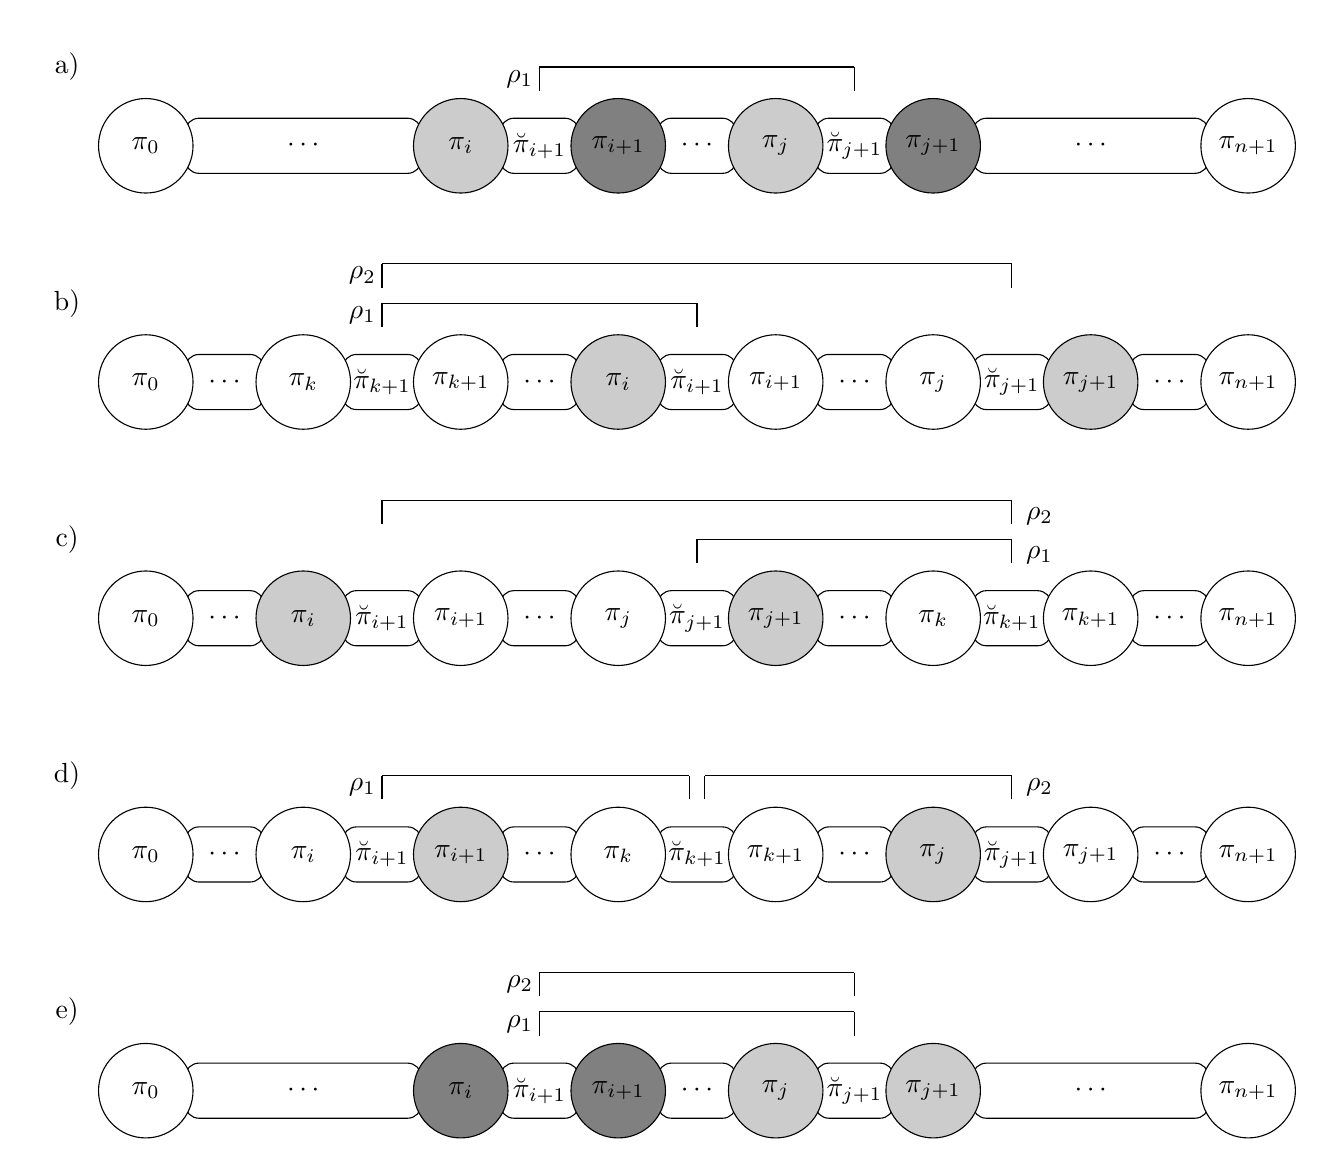
\begin{tikzpicture}
      %%%%% a)

      \node[draw=none,fill=none, minimum height=1cm, minimum width=1cm] at (-3.0, 1.0) {a)};

      % intergenic regions
      \node[rectangle,draw,fill=white!20, minimum height=.7cm, minimum width=3cm, rounded corners=5pt] at (0.0, 0.0) {$\cdots$};
      \node[rectangle,draw,fill=white!20, minimum height=.7cm, minimum width=1cm, rounded corners=5pt] at (3.0, 0.0) {$\breve\pi_{i+1}$};
      \node[rectangle,draw,fill=white!20, minimum height=.7cm, minimum width=1cm, rounded corners=5pt] at (5.0, 0.0) {$\cdots$};
      \node[rectangle,draw,fill=white!20, minimum height=.7cm, minimum width=1cm, rounded corners=5pt] at (7.0, 0.0) {$\breve\pi_{j+1}$};
      \node[rectangle,draw,fill=white!20, minimum height=.7cm, minimum width=3cm, rounded corners=5pt] at (10.0, 0.0) {$\cdots$};

      % genes
      \node[draw, circle, minimum height=1.2cm, minimum width=1.2cm, fill=white!20] at ({(2*0 - 2)}, 0.0) {$\pi_{0}$};
      \node[draw, circle, minimum height=1.2cm, minimum width=1.2cm, fill=black!20] at ({(2*2 - 2)}, 0.0) {$\pi_{i}$};
      \node[draw, circle, minimum height=1.2cm, minimum width=1.2cm, fill=black!50] at ({(2*3 - 2)}, 0.0) {$\pi_{i+1}$};
      \node[draw, circle, minimum height=1.2cm, minimum width=1.2cm, fill=black!20] at ({(2*4 - 2)}, 0.0) {$\pi_{j}$};
      \node[draw, circle, minimum height=1.2cm, minimum width=1.2cm, fill=black!50] at ({(2*5 - 2)}, 0.0) {$\pi_{j+1}$};
      \node[draw, circle, minimum height=1.2cm, minimum width=1.2cm, fill=white!20] at ({(2*7 - 2)}, 0.0) {$\pi_{n+1}$};

      % indexes
      \draw (3.0, 0.7) -- (3.0, 1.0);
      \draw (7.0, 0.7) -- (7.0, 1.0);
      \draw (3.0, 1.0) -- (7.0, 1.0);
      \node[draw=none,fill=none] at (2.75, 0.85) {$\rho_1$};

      %%%%% b)

      \node[draw=none,fill=none, minimum height=1cm, minimum width=1cm] at (-3.0, -2.0) {b)};

      % intergenic regions
      \node[rectangle,draw,fill=white!20, minimum height=.7cm, minimum width=1cm, rounded corners=5pt] at (-1.0, -3.0) {$\cdots$};
      \node[rectangle,draw,fill=white!20, minimum height=.7cm, minimum width=1cm, rounded corners=5pt] at (1.0, -3.0) {$\breve\pi_{k+1}$};
      \node[rectangle,draw,fill=white!20, minimum height=.7cm, minimum width=1cm, rounded corners=5pt] at (3.0, -3.0) {$\cdots$};
      \node[rectangle,draw,fill=white!20, minimum height=.7cm, minimum width=1cm, rounded corners=5pt] at (5.0, -3.0) {$\breve\pi_{i+1}$};
      \node[rectangle,draw,fill=white!20, minimum height=.7cm, minimum width=1cm, rounded corners=5pt] at (7.0, -3.0) {$\cdots$};
      \node[rectangle,draw,fill=white!20, minimum height=.7cm, minimum width=1cm, rounded corners=5pt] at (9.0, -3.0) {$\breve\pi_{j+1}$};
      \node[rectangle,draw,fill=white!20, minimum height=.7cm, minimum width=1cm, rounded corners=5pt] at (11.0, -3.0) {$\cdots$};

      % genes
      \node[draw, circle, minimum height=1.2cm, minimum width=1.2cm, fill=white!20] at ({(2*0 - 2)}, -3.0) {$\pi_{0}$};
      \node[draw, circle, minimum height=1.2cm, minimum width=1.2cm, fill=white!20] at ({(2*1 - 2)}, -3.0) {$\pi_{k}$};
      \node[draw, circle, minimum height=1.2cm, minimum width=1.2cm, fill=white!20] at ({(2*2 - 2)}, -3.0) {$\pi_{k+1}$};
      \node[draw, circle, minimum height=1.2cm, minimum width=1.2cm, fill=black!20] at ({(2*3 - 2)}, -3.0) {$\pi_{i}$};
      \node[draw, circle, minimum height=1.2cm, minimum width=1.2cm, fill=white!20] at ({(2*4 - 2)}, -3.0) {$\pi_{i+1}$};
      \node[draw, circle, minimum height=1.2cm, minimum width=1.2cm, fill=white!20] at ({(2*5 - 2)}, -3.0) {$\pi_{j}$};
      \node[draw, circle, minimum height=1.2cm, minimum width=1.2cm, fill=black!20] at ({(2*6 - 2)}, -3.0) {$\pi_{j+1}$};
      \node[draw, circle, minimum height=1.2cm, minimum width=1.2cm, fill=white!20] at ({(2*7 - 2)}, -3.0) {$\pi_{n+1}$};

      % indexes
      \draw (1.0, -2.3) -- (1.0, -2.0);
      \draw (5.0, -2.3) -- (5.0, -2.0);
      \draw (1.0, -2.0) -- (5.0, -2.0);
      \node[draw=none,fill=none] at (0.75, -2.15) {$\rho_1$};

      \draw (9.0, -1.8) -- (9.0, -1.5);
      \draw (1.0, -1.8) -- (1.0, -1.5);
      \draw (1.0, -1.5) -- (9.0, -1.5);
      \node[draw=none,fill=none] at (0.75, -1.65) {$\rho_2$};

      %%%%% c)

      \node[draw=none,fill=none, minimum height=1cm, minimum width=1cm] at (-3.0, -5.0) {c)};

      % intergenic regions
      \node[rectangle,draw,fill=white!20, minimum height=.7cm, minimum width=1cm, rounded corners=5pt] at (-1.0, -6.0) {$\cdots$};
      \node[rectangle,draw,fill=white!20, minimum height=.7cm, minimum width=1cm, rounded corners=5pt] at (1.0, -6.0) {$\breve\pi_{i+1}$};
      \node[rectangle,draw,fill=white!20, minimum height=.7cm, minimum width=1cm, rounded corners=5pt] at (3.0, -6.0) {$\cdots$};
      \node[rectangle,draw,fill=white!20, minimum height=.7cm, minimum width=1cm, rounded corners=5pt] at (5.0, -6.0) {$\breve\pi_{j+1}$};
      \node[rectangle,draw,fill=white!20, minimum height=.7cm, minimum width=1cm, rounded corners=5pt] at (7.0, -6.0) {$\cdots$};
      \node[rectangle,draw,fill=white!20, minimum height=.7cm, minimum width=1cm, rounded corners=5pt] at (9.0, -6.0) {$\breve\pi_{k+1}$};
      \node[rectangle,draw,fill=white!20, minimum height=.7cm, minimum width=1cm, rounded corners=5pt] at (11.0, -6.0) {$\cdots$};

      % genes
      \node[draw, circle, minimum height=1.2cm, minimum width=1.2cm, fill=white!20] at ({(2*0 - 2)}, -6.0) {$\pi_{0}$};
      \node[draw, circle, minimum height=1.2cm, minimum width=1.2cm, fill=black!20] at ({(2*1 - 2)}, -6.0) {$\pi_{i}$};
      \node[draw, circle, minimum height=1.2cm, minimum width=1.2cm, fill=white!20] at ({(2*2 - 2)}, -6.0) {$\pi_{i+1}$};
      \node[draw, circle, minimum height=1.2cm, minimum width=1.2cm, fill=white!20] at ({(2*3 - 2)}, -6.0) {$\pi_{j}$};
      \node[draw, circle, minimum height=1.2cm, minimum width=1.2cm, fill=black!20] at ({(2*4 - 2)}, -6.0) {$\pi_{j+1}$};
      \node[draw, circle, minimum height=1.2cm, minimum width=1.2cm, fill=white!20] at ({(2*5 - 2)}, -6.0) {$\pi_{k}$};
      \node[draw, circle, minimum height=1.2cm, minimum width=1.2cm, fill=white!20] at ({(2*6 - 2)}, -6.0) {$\pi_{k+1}$};
      \node[draw, circle, minimum height=1.2cm, minimum width=1.2cm, fill=white!20] at ({(2*7 - 2)}, -6.0) {$\pi_{n+1}$};

      % indexes
      \draw (5.0, -5.3) -- (5.0, -5.0);
      \draw (9.0, -5.3) -- (9.0, -5.0);
      \draw (5.0, -5.0) -- (9.0, -5.0);
      \node[draw=none,fill=none] at (9.35, -5.2) {$\rho_1$};

      \draw (9.0, -4.8) -- (9.0, -4.5);
      \draw (1.0, -4.8) -- (1.0, -4.5);
      \draw (1.0, -4.5) -- (9.0, -4.5);
      \node[draw=none,fill=none] at (9.35, -4.7) {$\rho_2$};

      %%%%% d)

      \node[draw=none,fill=none, minimum height=1cm, minimum width=1cm] at (-3.0, -8.0) {d)};

      % intergenic regions
      \node[rectangle,draw,fill=white!20, minimum height=.7cm, minimum width=1cm, rounded corners=5pt] at (-1.0, -9.0) {$\cdots$};
      \node[rectangle,draw,fill=white!20, minimum height=.7cm, minimum width=1cm, rounded corners=5pt] at (1.0, -9.0) {$\breve\pi_{i+1}$};
      \node[rectangle,draw,fill=white!20, minimum height=.7cm, minimum width=1cm, rounded corners=5pt] at (3.0, -9.0) {$\cdots$};
      \node[rectangle,draw,fill=white!20, minimum height=.7cm, minimum width=1cm, rounded corners=5pt] at (5.0, -9.0) {$\breve\pi_{k+1}$};
      \node[rectangle,draw,fill=white!20, minimum height=.7cm, minimum width=1cm, rounded corners=5pt] at (7.0, -9.0) {$\cdots$};
      \node[rectangle,draw,fill=white!20, minimum height=.7cm, minimum width=1cm, rounded corners=5pt] at (9.0, -9.0) {$\breve\pi_{j+1}$};
      \node[rectangle,draw,fill=white!20, minimum height=.7cm, minimum width=1cm, rounded corners=5pt] at (11.0, -9.0) {$\cdots$};

      % genes
      \node[draw, circle, minimum height=1.2cm, minimum width=1.2cm, fill=white!20] at ({(2*0 - 2)}, -9.0) {$\pi_{0}$};
      \node[draw, circle, minimum height=1.2cm, minimum width=1.2cm, fill=white!20] at ({(2*1 - 2)}, -9.0) {$\pi_{i}$};
      \node[draw, circle, minimum height=1.2cm, minimum width=1.2cm, fill=black!20] at ({(2*2 - 2)}, -9.0) {$\pi_{i+1}$};
      \node[draw, circle, minimum height=1.2cm, minimum width=1.2cm, fill=white!20] at ({(2*3 - 2)}, -9.0) {$\pi_{k}$};
      \node[draw, circle, minimum height=1.2cm, minimum width=1.2cm, fill=white!20] at ({(2*4 - 2)}, -9.0) {$\pi_{k+1}$};
      \node[draw, circle, minimum height=1.2cm, minimum width=1.2cm, fill=black!20] at ({(2*5 - 2)}, -9.0) {$\pi_{j}$};
      \node[draw, circle, minimum height=1.2cm, minimum width=1.2cm, fill=white!20] at ({(2*6 - 2)}, -9.0) {$\pi_{j+1}$};
      \node[draw, circle, minimum height=1.2cm, minimum width=1.2cm, fill=white!20] at ({(2*7 - 2)}, -9.0) {$\pi_{n+1}$};

      % indexes
      \draw (1.0, -8.3) -- (1.0, -8.0);
      \draw (4.9, -8.3) -- (4.9, -8.0);
      \draw (1.0, -8.0) -- (4.9, -8.0);
      \node[draw=none,fill=none] at (0.75, -8.15) {$\rho_1$};

      \draw (5.1, -8.3) -- (5.1, -8.0);
      \draw (9.0, -8.3) -- (9.0, -8.0);
      \draw (5.1, -8.0) -- (9.0, -8.0);
      \node[draw=none,fill=none] at (9.35, -8.15) {$\rho_2$};

      %%%%% e)

      \node[draw=none,fill=none, minimum height=1cm, minimum width=1cm] at (-3.0, -11.0) {e)};

      % intergenic regions
      \node[rectangle,draw,fill=white!20, minimum height=.7cm, minimum width=3cm, rounded corners=5pt] at (0.0, -12.0) {$\cdots$};
      \node[rectangle,draw,fill=white!20, minimum height=.7cm, minimum width=1cm, rounded corners=5pt] at (3.0, -12.0) {$\breve\pi_{i+1}$};
      \node[rectangle,draw,fill=white!20, minimum height=.7cm, minimum width=1cm, rounded corners=5pt] at (5.0, -12.0) {$\cdots$};
      \node[rectangle,draw,fill=white!20, minimum height=.7cm, minimum width=1cm, rounded corners=5pt] at (7.0, -12.0) {$\breve\pi_{j+1}$};
      \node[rectangle,draw,fill=white!20, minimum height=.7cm, minimum width=3cm, rounded corners=5pt] at (10.0, -12.0) {$\cdots$};

      % genes
      \node[draw, circle, minimum height=1.2cm, minimum width=1.2cm, fill=white!20] at ({(2*0 - 2)}, -12.0) {$\pi_{0}$};
      \node[draw, circle, minimum height=1.2cm, minimum width=1.2cm, fill=black!50] at ({(2*2 - 2)}, -12.0) {$\pi_{i}$};
      \node[draw, circle, minimum height=1.2cm, minimum width=1.2cm, fill=black!50] at ({(2*3 - 2)}, -12.0) {$\pi_{i+1}$};
      \node[draw, circle, minimum height=1.2cm, minimum width=1.2cm, fill=black!20] at ({(2*4 - 2)}, -12.0) {$\pi_{j}$};
      \node[draw, circle, minimum height=1.2cm, minimum width=1.2cm, fill=black!20] at ({(2*5 - 2)}, -12.0) {$\pi_{j+1}$};
      \node[draw, circle, minimum height=1.2cm, minimum width=1.2cm, fill=white!20] at ({(2*7 - 2)}, -12.0) {$\pi_{n+1}$};

      % indexes
      \draw (3.0, -11.3) -- (3.0, -11.0);
      \draw (7.0, -11.3) -- (7.0, -11.0);
      \draw (3.0, -11.0) -- (7.0, -11.0);
      \node[draw=none,fill=none] at (2.75, -11.15) {$\rho_1$};

      \draw (3.0, -10.8) -- (3.0, -10.5);
      \draw (7.0, -10.8) -- (7.0, -10.5);
      \draw (3.0, -10.5) -- (7.0, -10.5);
      \node[draw=none,fill=none] at (2.75, -10.65) {$\rho_2$};
    \end{tikzpicture}
  }
  \caption[Possibilidades de remoção de, pelo menos, um breakpoint tipo um a partir de pares de breakpoints conectados.]{Possibilidades que podem surgir quando existe um par de breakpoints conectados e reversões que podem ser aplicadas para remover, pelo menos, um breakpoint tipo um. O par de elementos consecutivos no genoma alvo está representado por tons de cinza.}
  \label{figure:EMTPDAVS}
\end{figure}

Considere o Algoritmo~\ref{algorithm:AKKUXQNR} para a variação sem sinais do problema \SbIR{}.  

\begin{algorithm}[!tbh]
  \caption{Um algoritmo de aproximação para o problema \SbIR{}.\label{algorithm:AKKUXQNR}}
  \Entrada{Uma instância intergênica rígida balanceada sem sinais $\mathcal{I}=((\pi,\breve\pi),(\iota,\breve\iota))$}
  \Saida{Uma sequência de reversões $S$, tal que $(\pi,\breve\pi) \cdot S = (\iota,\breve\iota)$}
    Seja $S \gets ()$ \\
    \Enqto{$ib_1(\mathcal{I}) > 1$}{
      \tcp{Lema~\ref{lemma:WYEZMYTM}}
      $(\pi_i,\pi_{i+1})$, $(\pi_j,\pi_{j+1}) \gets $ encontre um par de breakpoints conectados \\
      \tcp{Lema~\ref{lemma:IMYFBWDY}}
      \Se{$(\pi_i,\pi_{i+1})$, $(\pi_j,\pi_{j+1})$ pertence ao caso $(i)$}{
        $S' \gets (\rho_1)$ \\
      }\SenaoSe{$(\pi_i,\pi_{i+1})$, $(\pi_j,\pi_{j+1})$ pertence ao caso $(ii)$}{
        $S' \gets (\rho_1,\rho_2)$ \\
      }\SenaoSe{$(\pi_i,\pi_{i+1})$, $(\pi_j,\pi_{j+1})$ pertence ao caso $(iii)$}{
        $S' \gets (\rho_1,\rho_2)$ \\
      }\SenaoSe{$(\pi_i,\pi_{i+1})$, $(\pi_j,\pi_{j+1})$ pertence ao caso $(iv)$}{
        $S' \gets (\rho_1,\rho_2)$ \\
      }
      $S \gets S + S'$ \\
      $\mathcal{I} \gets ((\pi, \breve\pi) \cdot S',(\iota,\breve\iota))$ \\
    }
  \Retorna{S}
\end{algorithm}

\begin{lemma}\label{lemma:RBHACFIP}
Seja $\mathcal{I}=((\pi,\breve\pi),(\iota,\breve\iota))$ uma instância intergênica rígida balanceada sem sinais. O Algoritmo~\ref{algorithm:AKKUXQNR} transforma $(\pi,\breve\pi)$ em $(\iota,\breve\iota)$ utilizando, no máximo, $2ib_1(\mathcal{I})$ reversões.
\end{lemma}
\begin{proof}
  No Algoritmo~\ref{algorithm:AKKUXQNR}, temos que enquanto $ib_1(\mathcal{I})$ for maior que um, ou seja, $(\pi,\breve\pi)$ for diferente de $(\iota,\breve\iota)$ (pela Observação~\ref{remark:UDYJTHAH} e Lema~\ref{lemma:WSPRPLAH}), o seguinte procedimento é aplicado: pelos lemas~\ref{lemma:WYEZMYTM} e~\ref{lemma:IMYFBWDY}, sempre podemos encontrar um par conectado de breakpoints e remover, pelo menos, um breakpoint tipo um após aplicar duas reversões, no máximo. A cada iteração do algoritmo, pelo menos um breakpoint tipo um é removido. Dessa forma, o genoma alvo eventualmente será alcançado. No pior caso, cada breakpoint tipo um é removido utilizando duas reversões, e $2ib_1(\mathcal{I})$ reversões são utilizadas para transformar $(\pi,\breve\pi)$ em $(\iota,\breve\iota)$. Logo, o lema segue.
\end{proof}

Note que o Algoritmo~\ref{algorithm:AKKUXQNR} pode ser analisado considerando os seguintes pontos: 
\begin{itemize}
  \item Encontrar o par conectado de breakpoints, que pode ser feito em tempo linear com o auxílio da permutação inversa de $\pi$.
  \item Aplicação dos casos do Lema~\ref{lemma:IMYFBWDY}, que no pior caso também pode levar um tempo linear se for necessário encontrar o breakpoint tipo um $(\pi_k,\pi_{k+1})$ nos casos $(ii)$ e $(iii)$. 
\end{itemize}

Como esse processo é repetido $n$ vezes, no máximo, então o tempo de execução do Algoritmo~\ref{algorithm:AKKUXQNR} é $\mathcal{O}(n^2)$.

\begin{theorem}\label{theorem:BLJAGNDZ}
O Algoritmo~\ref{algorithm:AKKUXQNR} é uma $4$-aproximação para a variação sem sinais do problema \SbIR{}.
\end{theorem}
\begin{proof}
Seja $\mathcal{I}=((\pi,\breve\pi),(\iota,\breve\iota))$ uma instância intergênica rígida balanceada sem sinais. Pelo Lema~\ref{lemma:RBHACFIP}, o Algoritmo~\ref{algorithm:AKKUXQNR} transforma $(\pi,\breve\pi)$ em $(\iota,\breve\iota)$ utilizando, no máximo, $2ib_1(\mathcal{I})$ reversões. Pelo Teorema~\ref{theorem:MPFPKHQO}, temos o seguinte limitante inferior: $di_{\R}(\mathcal{I}) \ge \frac{ib_1(\mathcal{I})}{2}$. Logo, o teorema segue. 
\end{proof}

% ------------------------------------------------------------------ %
\subsubsection{Reversão e Indel}
% ------------------------------------------------------------------ %

Nesta seção, apresentaremos um algoritmo de aproximação com fator $4$ para a variação sem sinais do problema \SbIRI{}.

\begin{lemma}\label{lemma:QGOIQLZD}
Seja $\mathcal{I}=((\pi,\breve\pi),(\iota,\breve\iota))$ uma instância intergênica rígida desbalanceada sem sinais tal que $\sum_{i=1}^{n+1}\breve\pi_i < \sum_{i=1}^{n+1}\breve\iota_i$. É sempre possível aplicar um indel $\delta$ de forma que $\Delta ib_1(\mathcal{I}, S=(\delta)) \le 0$ e $\mathcal{I}$ torna-se uma instância intergênica rígida balanceada.
\end{lemma}
\begin{proof}
Como $\mathcal{I}$ é desbalanceada, então $ib_1(\mathcal{I}) > 0$. Seja $(\pi_i,\pi_{i+1})$ um breakpoint tipo um de $\mathcal{I}$. Aplique o indel $\delta_{(x)}^{(i+1)}$, tal que $x = \sum_{i=1}^{n+1}\breve\iota_i - \sum_{i=1}^{n+1}\breve\pi_i$. Note que o indel insere a quantidade necessária de nucleotídeos na região intergênica $\breve\pi_{i+1}$ para tornar $\mathcal{I}$ uma instância balanceada. No pior caso, $(\pi_i,\pi_{i+1})$ continua sendo um breakpoint tipo um e o lema segue.
\end{proof}

\begin{lemma}\label{lemma:QNHGBLYF}
Seja $\mathcal{I}=((\pi,\breve\pi),(\iota,\breve\iota))$ uma instância intergênica rígida desbalanceada sem sinais tal que $ib_1(\mathcal{I}) = 1$. É sempre possível aplicar um indel $\delta$ de forma que $\Delta ib_1(\mathcal{I}, S=(\delta)) = -1$.
\end{lemma}
\begin{proof}
Seja $(\pi_i,\pi_{i+1})$ o único breakpoint tipo um de $\mathcal{I}$. Como $(\pi_i,\pi_{i+1})$ é único breakpoint tipo um de $\mathcal{I}$, então ele deve ser um breakpoint forte, obrigatoriamente (Lema~\ref{lemma:EFGATDBA}). Aplique o indel $\delta_{(x)}^{(i+1)}$, tal que $x = \breve\iota_{i+1} - \breve\pi_{i+1}$. Note que o indel insere ou remove a quantidade necessária de nucleotídeos na região intergênica $\breve\pi_{i+1}$ para remover o breakpoint $(\pi_i,\pi_{i+1})$ caso ele seja subcarregado ou sobrecarregado, respectivamente. O breakpoint $(\pi_i,\pi_{i+1})$ é removido após a aplicação do evento de indel e o lema segue.
\end{proof}

Considere o Algoritmo~\ref{algorithm:LHOPSFVN} para a variação sem sinais do problema \SbIRI{}.

\begin{algorithm}[!tbh]
  \caption{Um algoritmo de aproximação para o problema \SbIRI{}.\label{algorithm:LHOPSFVN}}
  \Entrada{Uma instância intergênica rígida sem sinais $\mathcal{I}=((\pi,\breve\pi),(\iota,\breve\iota))$}
  \Saida{Uma sequência de reversões e indels $S$, tal que $(\pi,\breve\pi) \cdot S = (\iota,\breve\iota)$}
    Seja $S \gets ()$ \\
    \tcp{Lema~\ref{lemma:QGOIQLZD}}
    \Se{$\sum_{i=1}^{n+1}\breve\pi_i < \sum_{i=1}^{n+1}\breve\iota_i$}{
      $S' \gets (\delta_1)$ \\
      $S \gets S + S'$ \\
      $\mathcal{I} \gets ((\pi, \breve\pi) \cdot S',(\iota,\breve\iota))$ \\
    }
    \Enqto{$ib(\mathcal{I}) > 1$}{
      \tcp{Lema~\ref{lemma:WYEZMYTM}}
      $(\pi_i,\pi_{i+1})$, $(\pi_j,\pi_{j+1}) \gets $ encontre um par de breakpoints conectados \\
      \tcp{Lema~\ref{lemma:IMYFBWDY}}
      \Se{$(\pi_i,\pi_{i+1})$, $(\pi_j,\pi_{j+1})$ pertence ao caso $(i)$}{
        $S' \gets (\rho_1)$ \\
      }\SenaoSe{$(\pi_i,\pi_{i+1})$, $(\pi_j,\pi_{j+1})$ pertence ao caso $(ii)$}{
        $S' \gets (\rho_1,\rho_2)$ \\
      }\SenaoSe{$(\pi_i,\pi_{i+1})$, $(\pi_j,\pi_{j+1})$ pertence ao caso $(iii)$}{
        $S' \gets (\rho_1,\rho_2)$ \\
      }\SenaoSe{$(\pi_i,\pi_{i+1})$, $(\pi_j,\pi_{j+1})$ pertence ao caso $(iv)$}{
        $S' \gets (\rho_1,\rho_2)$ \\
      }
      $S \gets S + S'$ \\
      $\mathcal{I} \gets ((\pi, \breve\pi) \cdot S',(\iota,\breve\iota))$ \\
    }
    \tcp{Lema~\ref{lemma:QNHGBLYF}}
    \Se{$ib(\mathcal{I}) = 1$}{
      $S' \gets (\delta_1)$ \\
      $S \gets S + S'$ \\
      $\mathcal{I} \gets ((\pi, \breve\pi) \cdot S',(\iota,\breve\iota))$ \\
    }
  \Retorna{S}
\end{algorithm}

\begin{lemma}\label{lemma:XUDIVWPC}
Seja $\mathcal{I}=((\pi,\breve\pi),(\iota,\breve\iota))$ uma instância intergênica rígida sem sinais. O Algoritmo~\ref{algorithm:LHOPSFVN} transforma $(\pi,\breve\pi)$ em $(\iota,\breve\iota)$ utilizando, no máximo, $2ib_1(\mathcal{I})$ eventos de reversão e indel.
\end{lemma}
\begin{proof}
  Podemos analisar o Algoritmo~\ref{algorithm:LHOPSFVN} considerando três cenários:
  \begin{itemize}
    \item $\sum_{i=1}^{n+1}\breve\pi_i < \sum_{i=1}^{n+1}\breve\iota_i$: nesse cenário o Algoritmo~\ref{algorithm:LHOPSFVN} aplica um indel (linhas 2-5) que pode não remover nenhum breakpoint tipo um, mas transforma $\mathcal{I}$ em uma instância balanceada. Caso ainda existam breakpoints em $\mathcal{I}$, então o laço de repetição (linhas 6-17) remove, por iteração, pelo menos um breakpoint tipo um utilizando, no máximo, duas reversões. Esse processo se repete até que todos os breakpoints tipo um de $\mathcal{I}$ sejam removidos. Como todos os breakpoints tipo um são removidos, então $(\pi,\breve\pi)$ é transformada em $(\iota,\breve\iota)$. Note que, se o indel aplicado inicialmente não remover nenhum breakpoint tipo um, então pelo menos uma reversão é aplicada em seguida. Além disso, pelo Lema~\ref{lemma:WSPRPLAH}, podemos deduzir que a última reversão que transforma $(\pi,\breve\pi)$ em $(\iota,\breve\iota)$ deve, obrigatoriamente, remover dois breakpoints tipo um. Isso implica que, no máximo, $2ib_1(\mathcal{I})$ reversões e indels são utilizadas pelo Algoritmo~\ref{algorithm:LHOPSFVN} para transformar $(\pi,\breve\pi)$ em $(\iota,\breve\iota)$.
    \item $\sum_{i=1}^{n+1}\breve\pi_i = \sum_{i=1}^{n+1}\breve\iota_i$: para esse cenário o Algoritmo~\ref{algorithm:LHOPSFVN} comporta-se exatamente como o Algoritmo~\ref{algorithm:AKKUXQNR}, que transforma $(\pi,\breve\pi)$ em $(\iota,\breve\iota)$ utilizando, no máximo, $2ib_1(\mathcal{I})$ reversões.
    \item $\sum_{i=1}^{n+1}\breve\pi_i > \sum_{i=1}^{n+1}\breve\iota_i$: nesse último cenário enquanto $ib_1(\mathcal{I})$ for maior que um, o Algoritmo~\ref{algorithm:LHOPSFVN} aplica, no máximo, duas reversões a cada iteração do laço de repetição (linhas 6-17) que removem, pelo menos, um breakpoint tipo um. Por fim, um indel é aplicado (linhas 19-22) removendo o último breakpoint tipo um e transformando $(\pi,\breve\pi)$ em $(\iota,\breve\iota)$.
  \end{itemize}
  Nos três cenários, o Algoritmo~\ref{algorithm:LHOPSFVN} transforma $(\pi,\breve\pi)$ em $(\iota,\breve\iota)$ utilizando, no máximo, $2ib_1(\mathcal{I})$ reversões e indels. Logo, o lema segue.
\end{proof}

Note que o Algoritmo~\ref{algorithm:LHOPSFVN} difere do Algoritmo~\ref{algorithm:AKKUXQNR} pelos trechos responsáveis por aplicar uma operação de indel (linhas 2-5 e 19-22). Ambos os trechos podem ser realizados em tempo linear. Dessa forma, o tempo de execução do Algoritmo~\ref{algorithm:LHOPSFVN} também é $\mathcal{O}(n^2)$.

\begin{theorem}\label{theorem:AFAHUIUF}
O Algoritmo~\ref{algorithm:LHOPSFVN} é uma $4$-aproximação para a variação sem sinais do problema \SbIRI{}.
\end{theorem}
\begin{proof}
Seja $\mathcal{I} = ((\pi,\breve\pi),(\iota,\breve\iota))$ uma instância intergênica rígida sem sinais. Pelo Lema~\ref{lemma:XUDIVWPC}, o Algoritmo~\ref{algorithm:LHOPSFVN} transforma $(\pi,\breve\pi)$ em $(\iota,\breve\iota)$ utilizando, no máximo, $2ib_1(\mathcal{I})$ eventos de reversão e indel. Pelo Teorema~\ref{theorem:MPFPKHQO}, temos o seguinte limitante inferior: $di_{\RI}(\mathcal{I}) \ge \frac{ib_1(\mathcal{I})}{2}$. Logo, o teorema segue. 
\end{proof}

% ------------------------------------------------------------------ %
\subsubsection{Reversão e Move}
% ------------------------------------------------------------------ %

Nesta seção, apresentaremos um algoritmo de aproximação com fator $4$ para a variação sem sinais do problema \SbIRM{}.

\begin{lemma}\label{lemma:NWNNZGXH}
Seja $\mathcal{I} = ((\pi,\breve\pi),(\iota,\breve\iota))$ uma instância intergênica rígida sem sinais e sejam $(\pi_i,\pi_{i+1})$ e $(\pi_j,\pi_{j+1})$ um par conectado de breakpoints. É possível remover pelo menos um breakpoint tipo um de $\mathcal{I}$ utilizando, no máximo, duas reversões ou um move.
\end{lemma}
\begin{proof}
Note que a aplicação do Lema~\ref{lemma:IMYFBWDY} já é suficiente para provar este lema. Entretanto, iremos melhorar o caso $(iv)$ para utilizarmos apenas um evento de move ao invés de duas reversões. Sem perda de generalidade, assuma que $i < j$. Como o par de breakpoints $(\pi_i,\pi_{i+1})$ e $(\pi_j,\pi_{j+1})$ está conectado, por definição, um dos seguintes casos deve ocorrer:
\begin{enumerate}[i.]
  \item O par de elementos $(\pi_i,\pi_{j})$ ou $(\pi_{i+1},\pi_{j+1})$ não forma uma adjacência intergênica, sendo os elementos consecutivos em $\iota$ e $\breve\pi_{i+1} + \breve\pi_{j+1} \ge \breve\iota_k$, onde $\breve\iota_k$ é o tamanho da região intergênica entre o par de elementos consecutivos em $\iota$. Aplique uma reversão como descrito no caso $(i)$ do Lema~\ref{lemma:IMYFBWDY}.   
  \item O par  de elementos $(\pi_i,\pi_{j+1})$ não forma uma adjacência intergênica, sendo os elementos consecutivos em $\iota$ e $\breve\pi_{i+1} + \breve\pi_{j+1} \ge \breve\iota_k$, onde $\breve\iota_k$ é o tamanho da região intergênica entre o par de elementos consecutivos em $\iota$. Aplique uma sequência de duas reversões como descrito no caso $(ii)$ do Lema~\ref{lemma:IMYFBWDY}.
  \item O par de elementos $(\pi_{i+1},\pi_{j})$ não forma uma adjacência intergênica, sendo os elementos consecutivos em $\iota$ e $\breve\pi_{i+1} + \breve\pi_{j+1} \ge \breve\iota_k$, onde $\breve\iota_k$ é o tamanho da região intergênica entre o par de elementos consecutivos em $\iota$. Aplique uma sequência de duas reversões como descrito no caso $(iii)$ do Lema~\ref{lemma:IMYFBWDY}.
  \item O par de elementos $(\pi_{i},\pi_{i+1})$ ou $(\pi_{j},\pi_{j+1})$ não forma uma adjacência intergênica, sendo os elementos consecutivos em $\iota$ e $\breve\pi_{i+1} + \breve\pi_{j+1} \ge \breve\iota_k$, onde $\breve\iota_k$ é o tamanho da região intergênica entre o par de elementos consecutivos em $\iota$. Note que, pela definição, $(\pi_{i},\pi_{i+1})$ ou $(\pi_{j},\pi_{j+1})$ é um breakpoint forte. Se $(\pi_{i},\pi_{i+1})$ for um breakpoint forte, então ele pode ser sobrecarregado ou subcarregado. Caso ele seja sobrecarregado, então aplicamos um move $\mu^{(i+1,j+1)}_{(x)}$, tal que $x = \breve\pi_{i+1} - \breve\iota_{max(\pi_{i},\pi_{i+1})}$. Caso contrário, aplicamos um move $\mu^{(j+1,i+1)}_{(x)}$, tal que $x = \breve\iota_{max(\pi_{i},\pi_{i+1})} - \breve\pi_{i+1}$. De maneira similar, se $(\pi_{j},\pi_{j+1})$ for um breakpoint forte, então ele pode ser sobrecarregado ou subcarregado. Caso ele seja sobrecarregado, então aplicamos um move $\mu^{(j+1,i+1)}_{(x)}$, tal que $x = \breve\pi_{j+1} - \breve\iota_{max(\pi_{j},\pi_{j+1})}$. Caso contrário, aplicamos um move $\mu^{(i+1,j+1)}_{(x)}$, tal que $x = \breve\iota_{max(\pi_{j},\pi_{j+1})} - \breve\pi_{j+1}$. Em ambos os cenários, pelo menos um breakpoint tipo um é removido após a aplicação do move (Figura~\ref{figure:CAIZFSWA}).
\end{enumerate}
Note que o caso $(i)$ aplica apenas uma reversão e remove, pelo menos, um breakpoint tipo um. Os casos $(ii)$ e $(iii)$ aplicam inicialmente uma reversão que não remove nenhum breakpoint tipo um, mas garante que nenhum novo breakpoint é gerado e que o caso $(i)$ poderá ser aplicado em seguida. Por fim, o caso $(iv)$ remove, pelo menos, um breakpoint tipo um utilizando um move. No pior caso, duas reversões são aplicadas e, pelo menos, um breakpoint tipo um é removido de $\mathcal{I}$. Logo, o lema segue. 
\end{proof}

\begin{figure}[!tbh]
  \resizebox{\linewidth}{!}{
    \centering
    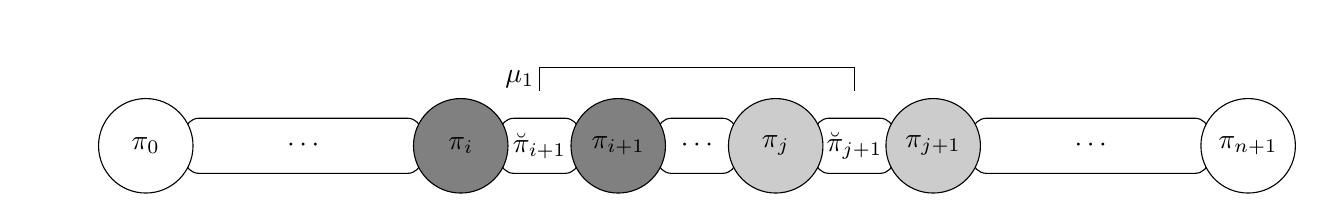
\begin{tikzpicture}
      %%%%% e)

      \node[draw=none,fill=none, minimum height=1cm, minimum width=1cm] at (-3.0, -11.0) {};

      % intergenic regions
      \node[rectangle,draw,fill=white!20, minimum height=.7cm, minimum width=3cm, rounded corners=5pt] at (0.0, -12.0) {$\cdots$};
      \node[rectangle,draw,fill=white!20, minimum height=.7cm, minimum width=1cm, rounded corners=5pt] at (3.0, -12.0) {$\breve\pi_{i+1}$};
      \node[rectangle,draw,fill=white!20, minimum height=.7cm, minimum width=1cm, rounded corners=5pt] at (5.0, -12.0) {$\cdots$};
      \node[rectangle,draw,fill=white!20, minimum height=.7cm, minimum width=1cm, rounded corners=5pt] at (7.0, -12.0) {$\breve\pi_{j+1}$};
      \node[rectangle,draw,fill=white!20, minimum height=.7cm, minimum width=3cm, rounded corners=5pt] at (10.0, -12.0) {$\cdots$};

      % genes
      \node[draw, circle, minimum height=1.2cm, minimum width=1.2cm, fill=white!20] at ({(2*0 - 2)}, -12.0) {$\pi_{0}$};
      \node[draw, circle, minimum height=1.2cm, minimum width=1.2cm, fill=black!50] at ({(2*2 - 2)}, -12.0) {$\pi_{i}$};
      \node[draw, circle, minimum height=1.2cm, minimum width=1.2cm, fill=black!50] at ({(2*3 - 2)}, -12.0) {$\pi_{i+1}$};
      \node[draw, circle, minimum height=1.2cm, minimum width=1.2cm, fill=black!20] at ({(2*4 - 2)}, -12.0) {$\pi_{j}$};
      \node[draw, circle, minimum height=1.2cm, minimum width=1.2cm, fill=black!20] at ({(2*5 - 2)}, -12.0) {$\pi_{j+1}$};
      \node[draw, circle, minimum height=1.2cm, minimum width=1.2cm, fill=white!20] at ({(2*7 - 2)}, -12.0) {$\pi_{n+1}$};

      % indexes
      \draw (3.0, -11.3) -- (3.0, -11.0);
      \draw (7.0, -11.3) -- (7.0, -11.0);
      \draw (3.0, -11.0) -- (7.0, -11.0);
      \node[draw=none,fill=none] at (2.75, -11.15) {$\mu_1$};
    \end{tikzpicture}
  }
  \caption[Exemplo de remoção de pelo menos um breakpoint tipo um após a aplicação de um move $\mu$.]{Exemplo de remoção de pelo menos um breakpoint tipo um após a aplicação de um move $\mu$.}
  \label{figure:CAIZFSWA}
\end{figure}

Considere o Algoritmo~\ref{algorithm:OLSRUEFZ} para a variação sem sinais do problema \SbIRM{}.  

\begin{algorithm}[!tbh]
  \caption{Um algoritmo de aproximação para o problema \SbIRM{}.\label{algorithm:OLSRUEFZ}}
  \Entrada{Uma instância intergênica rígida balanceada sem sinais $\mathcal{I}=((\pi,\breve\pi),(\iota,\breve\iota))$}
  \Saida{Uma sequência de reversões e moves $S$, tal que $(\pi,\breve\pi) \cdot S = (\iota,\breve\iota)$}
    Seja $S \gets ()$ \\
    \Enqto{$ib_1(\mathcal{I}) > 1$}{
      \tcp{Lema~\ref{lemma:WYEZMYTM}}
      $(\pi_i,\pi_{i+1})$, $(\pi_j,\pi_{j+1}) \gets $ encontre um par de breakpoints conectados \\
      \tcp{Lema~\ref{lemma:NWNNZGXH}}
      \Se{$(\pi_i,\pi_{i+1})$, $(\pi_j,\pi_{j+1})$ pertence ao caso $(i)$}{
        $S' \gets (\rho_1)$ \\
      }\SenaoSe{$(\pi_i,\pi_{i+1})$, $(\pi_j,\pi_{j+1})$ pertence ao caso $(iv)$}{
        $S' \gets (\mu_1)$ \\
      }
      \SenaoSe{$(\pi_i,\pi_{i+1})$, $(\pi_j,\pi_{j+1})$ pertence ao caso $(ii)$}{
        $S' \gets (\rho_1,\rho_2)$ \\
      }\SenaoSe{$(\pi_i,\pi_{i+1})$, $(\pi_j,\pi_{j+1})$ pertence ao caso $(iii)$}{
        $S' \gets (\rho_1,\rho_2)$ \\
      }
      $S \gets S + S'$ \\
      $\mathcal{I} \gets ((\pi, \breve\pi) \cdot S',(\iota,\breve\iota))$ \\
    }
  \Retorna{S}
\end{algorithm}

\begin{lemma}\label{lemma:TZYVWBRT}
Seja $\mathcal{I} = ((\pi,\breve\pi),(\iota,\breve\iota))$ uma instância intergênica rígida balanceada sem sinais. O Algoritmo~\ref{algorithm:OLSRUEFZ} transforma $(\pi,\breve\pi)$ em $(\iota,\breve\iota)$ utilizando, no máximo, $2ib_1(\mathcal{I})$ eventos de reversão e move.
\end{lemma}
\begin{proof}
  No Algoritmo~\ref{algorithm:OLSRUEFZ}, temos que enquanto $ib_1(\mathcal{I})$ for maior que um, ou seja, $(\pi,\breve\pi)$ for diferente de $(\iota,\breve\iota)$ (pela Observação~\ref{remark:UDYJTHAH} e Lema~\ref{lemma:WSPRPLAH}), o seguinte procedimento é aplicado: pelos lemas~\ref{lemma:WYEZMYTM} e~\ref{lemma:NWNNZGXH}, sempre podemos encontrar um par conectado de breakpoints e remover, pelo menos, um breakpoint tipo um após aplicar, no máximo, duas reversões ou um move. A cada iteração do algoritmo, pelo menos um breakpoint tipo um é removido. Dessa forma, o genoma alvo eventualmente será alcançado. No pior caso, cada breakpoint tipo um é removido utilizando dois eventos de rearranjo. Logo, uma sequência com, no máximo, $2ib_1(\mathcal{I})$ reversões e moves é utilizada para transformar $(\pi,\breve\pi)$ em $(\iota,\breve\iota)$ e o lema segue.
\end{proof}

Note que o Algoritmo~\ref{algorithm:OLSRUEFZ} difere do Algoritmo~\ref{algorithm:AKKUXQNR} apenas pelo caso $(iv)$ de um par conectado de breakpoints, que pode ser realizado em tempo constante. Logo, o tempo de execução do Algoritmo~\ref{algorithm:OLSRUEFZ} também é $\mathcal{O}(n^2)$.

\begin{theorem}\label{theorem:PNTKLAHZ}
O Algoritmo~\ref{algorithm:OLSRUEFZ} é uma $4$-aproximação para a variação sem sinais do problema \SbIRM{}.
\end{theorem}
\begin{proof}
Seja $\mathcal{I} = ((\pi,\breve\pi),(\iota,\breve\iota))$ uma instância intergênica rígida balanceada sem sinais. Pelo Lema~\ref{lemma:TZYVWBRT}, o Algoritmo~\ref{algorithm:OLSRUEFZ} transforma $(\pi,\breve\pi)$ em $(\iota,\breve\iota)$ utilizando, no máximo, $2ib_1(\mathcal{I})$ eventos de reversão e move. Pelo Teorema~\ref{theorem:MPFPKHQO}, temos o seguinte limitante inferior: $di_{\RM}(\mathcal{I}) \ge \frac{ib_1(\mathcal{I})}{2}$. Logo, o teorema segue. 
\end{proof}

% ------------------------------------------------------------------ %
\subsubsection{Reversão, Move e Indel}
% ------------------------------------------------------------------ %

Nesta seção, apresentaremos um algoritmo de aproximação com fator $4$ para a variação sem sinais do problema \SbIRMI{} (Algoritmo~\ref{algorithm:JAJGNYWD}).

\begin{algorithm}[!tbh]
  \caption{Um algoritmo de aproximação para o problema \SbIRMI{}.\label{algorithm:JAJGNYWD}}
  \Entrada{Uma instância intergênica rígida sem sinais $\mathcal{I}=((\pi,\breve\pi),(\iota,\breve\iota))$}
  \Saida{Uma sequência de reversões, moves e indels $S$, tal que $(\pi,\breve\pi) \cdot S = (\iota,\breve\iota)$}
    Seja $S \gets ()$ \\
    \tcp{Lema~\ref{lemma:QGOIQLZD}}
    \Se{$\sum_{i=1}^{n+1}\breve\pi_i < \sum_{i=1}^{n+1}\breve\iota_i$}{
      $S' \gets (\delta_1)$ \\
      $S \gets S + S'$ \\
      $\mathcal{I} \gets ((\pi, \breve\pi) \cdot S',(\iota,\breve\iota))$ \\
    }
    \Enqto{$ib(\mathcal{I}) > 1$}{
      \tcp{Lema~\ref{lemma:WYEZMYTM}}
      $(\pi_i,\pi_{i+1})$, $(\pi_j,\pi_{j+1}) \gets $ encontre um par de breakpoints conectados \\
      \tcp{Lema~\ref{lemma:NWNNZGXH}}
      \Se{$(\pi_i,\pi_{i+1})$, $(\pi_j,\pi_{j+1})$ pertence ao caso $(i)$}{
        $S' \gets (\rho_1)$ \\
      }\SenaoSe{$(\pi_i,\pi_{i+1})$, $(\pi_j,\pi_{j+1})$ pertence ao caso $(iv)$}{
        $S' \gets (\mu_1)$ \\
      }\SenaoSe{$(\pi_i,\pi_{i+1})$, $(\pi_j,\pi_{j+1})$ pertence ao caso $(ii)$}{
        $S' \gets (\rho_1,\rho_2)$ \\
      }\SenaoSe{$(\pi_i,\pi_{i+1})$, $(\pi_j,\pi_{j+1})$ pertence ao caso $(iii)$}{
        $S' \gets (\rho_1,\rho_2)$ \\
      }
      $S \gets S + S'$ \\
      $\mathcal{I} \gets ((\pi, \breve\pi) \cdot S',(\iota,\breve\iota))$ \\
    }
    \tcp{Lema~\ref{lemma:QNHGBLYF}}
    \Se{$ib(\mathcal{I}) = 1$}{
      $S' \gets (\delta_1)$ \\
      $S \gets S + S'$ \\
      $\mathcal{I} \gets ((\pi, \breve\pi) \cdot S',(\iota,\breve\iota))$ \\
    }
  \Retorna{S}
\end{algorithm}

\begin{lemma}\label{lemma:SINGKSVU}
Seja $\mathcal{I} = ((\pi,\breve\pi),(\iota,\breve\iota))$ uma instância intergênica rígida sem sinais. O Algoritmo~\ref{algorithm:JAJGNYWD} transforma $(\pi,\breve\pi)$ em $(\iota,\breve\iota)$ utilizando, no máximo, $2ib_1(\mathcal{I})$ eventos de reversão, move e indel.
\end{lemma}
\begin{proof}
  A prova é similar à descrita no Lema~\ref{lemma:XUDIVWPC}.
\end{proof}

Note que o Algoritmo~\ref{algorithm:JAJGNYWD}, em comparação com o Algoritmo~\ref{algorithm:LHOPSFVN}, difere apenas pelo caso $(iv)$ de um par conectado de breakpoints, que pode ser realizado em tempo constante. Logo, o tempo de execução do Algoritmo~\ref{algorithm:JAJGNYWD} também é $\mathcal{O}(n^2)$.

\begin{theorem}\label{theorem:WSCHLXXJ}
O Algoritmo~\ref{algorithm:JAJGNYWD} é uma $4$-aproximação para a variação sem sinais do problema \SbIRMI{}.
\end{theorem}
\begin{proof}
Seja $\mathcal{I}=((\pi,\breve\pi),(\iota,\breve\iota))$ uma instância intergênica rígida sem sinais. Pelo Lema~\ref{lemma:SINGKSVU}, o Algoritmo~\ref{algorithm:JAJGNYWD} transforma $(\pi,\breve\pi)$ em $(\iota,\breve\iota)$ utilizando, no máximo, $2ib_1(\mathcal{I})$ eventos de reversão, move e indel. Pelo Teorema~\ref{theorem:MPFPKHQO}, temos o seguinte limitante inferior: $di_{\RMI}(\mathcal{I}) \ge \frac{ib_1(\mathcal{I})}{2}$. Logo, o teorema segue. 
\end{proof}

% ------------------------------------------------------------------ %
\subsubsection{Reversão e Transposição}
% ------------------------------------------------------------------ %

Nesta seção, apresentaremos algoritmos para a variação sem sinais do problema \SbIRT{} com fatores de aproximação $6$, $4.5$ e $4$.


\begin{lemma}\label{lemma:SIAFJFDO}
Seja $\mathcal{I}=((\pi,\breve\pi),(\iota,\breve\iota))$ uma instância intergênica rígida sem sinais e sejam $(\pi_i,\pi_{i+1})$ e $(\pi_j,\pi_{j+1})$ um par conectado de breakpoints. É possível remover pelo menos um breakpoint tipo um de $\mathcal{I}$ utilizando, no máximo, duas reversões ou uma transposição.
\end{lemma}
\begin{proof}
Note que a aplicação do Lema~\ref{lemma:IMYFBWDY} já é suficiente para provar este lema. Entretanto, iremos melhorar os casos $(ii)$ e $(iii)$ para utilizarmos apenas um evento de transposição ao invés de duas reversões. Sem perda de generalidade, assuma que $i < j$. Como os breakpoints $(\pi_i,\pi_{i+1})$ e $(\pi_j,\pi_{j+1})$ estão conectados, por definição, um dos seguintes casos deve ocorrer:
\begin{enumerate}[i.]
  \item O par de elementos $(\pi_i,\pi_{j})$ ou $(\pi_{i+1},\pi_{j+1})$ não forma uma adjacência intergênica, sendo os elementos consecutivos em $\iota$ e $\breve\pi_{i+1} + \breve\pi_{j+1} \ge \breve\iota_k$, onde $\breve\iota_k$ é o tamanho da região intergênica entre o par de elementos consecutivos em $\iota$. Aplique uma reversão como descrito no caso $(i)$ do Lema~\ref{lemma:IMYFBWDY}.
  \item O par  de elementos $(\pi_i,\pi_{j+1})$ não forma uma adjacência intergênica, sendo os elementos consecutivos em $\iota$ e $\breve\pi_{i+1} + \breve\pi_{j+1} \ge \breve\iota_k$, onde $\breve\iota_k$ é o tamanho da região intergênica entre o par de elementos consecutivos em $\iota$. Nesse caso, sabemos que deve existir um breakpoint tipo um $(\pi_k, \pi_{k+1})$, tal que $k <i$ ou $k > j$ (caso $(ii)$, Lema~\ref{lemma:IMYFBWDY}). Se $k < i$, aplicamos uma transposição $\tau^{(k+1,i+1,j+1)}_{(x,y,z)}$ para posicionar o elemento $\pi_{i}$ no lado esquerdo do elemento $\pi_{j+1}$ (Figura~\ref{figure:WDJFPAXN}(a)). Se $k > j$, aplicamos uma transposição $\tau^{(i+1,j+1,k+1)}_{(x,y,z)}$ para posicionar o elemento $\pi_{j+1}$ no lado direito do elemento $\pi_{i}$ (Figura~\ref{figure:WDJFPAXN}(b)). Em ambos os cenários, temos que $\breve\pi_{i+1} + \breve\pi_{j+1} \ge \breve\iota_k$. Logo, os parâmetros $x$, $y$ e $z$ sempre podem ser escolhidos de forma que, ao posicionar lado a lado o par de elementos $(\pi_i,\pi_{j+1})$, o tamanho da região entre eles seja igual no genoma de origem e alvo.
  \item O par de elementos $(\pi_{i+1},\pi_{j})$ não forma uma adjacência intergênica, sendo os elementos consecutivos em $\iota$ e $\breve\pi_{i+1} + \breve\pi_{j+1} \ge \breve\iota_k$, onde $\breve\iota_k$ é o tamanho da região intergênica entre o par de elementos consecutivos em $\iota$. Nesse caso, sabemos que deve existir um breakpoint tipo um $(\pi_k, \pi_{k+1})$, tal que $i < k < j$ (caso $(iii)$, Lema~\ref{lemma:IMYFBWDY}). Após identificar o breakpoint tipo um $(\pi_k, \pi_{k+1})$, aplicamos a transposição $\tau^{(i+1,k+1,j+1)}_{(x,y,z)}$ para posicionar o elemento $\pi_{j}$ no lado esquerdo do elemento $\pi_{i+1}$ (Figura~\ref{figure:WDJFPAXN}(c)). Como $\breve\pi_{i+1} + \breve\pi_{j+1} \ge \breve\iota_k$, então os parâmetros $x$, $y$ e $z$ sempre podem ser escolhidos de forma que, ao posicionar lado a lado o par de elementos $(\pi_{i+1},\pi_{j})$, o tamanho da região entre eles seja igual no genoma de origem e alvo.
  \item O par de elementos $(\pi_{i},\pi_{i+1})$ ou $(\pi_{j},\pi_{j+1})$ não forma uma adjacência intergênica, sendo os elementos consecutivos em $\iota$ e $\breve\pi_{i+1} + \breve\pi_{j+1} \ge \breve\iota_k$, onde $\breve\iota_k$ é o tamanho da região intergênica entre o par de elementos consecutivos em $\iota$. Aplique uma sequência de duas reversões como descrito no caso $(iv)$ do Lema~\ref{lemma:IMYFBWDY}.
\end{enumerate}
Note que o caso $(i)$ aplica apenas uma reversão que remove pelo menos um breakpoint tipo um. Os casos $(ii)$ e $(iii)$ aplicam apenas uma transposição que remove pelo menos um breakpoint tipo um. Por fim, o caso $(iv)$ aplica duas reversões e remove pelo menos um breakpoint tipo um. No pior caso, duas reversões são aplicadas e, pelo menos, um breakpoint tipo um é removido de $\mathcal{I}$. Logo, o lema segue. 
\end{proof}

\begin{figure}[!tbh]
  \resizebox{\linewidth}{!}{
    \centering
    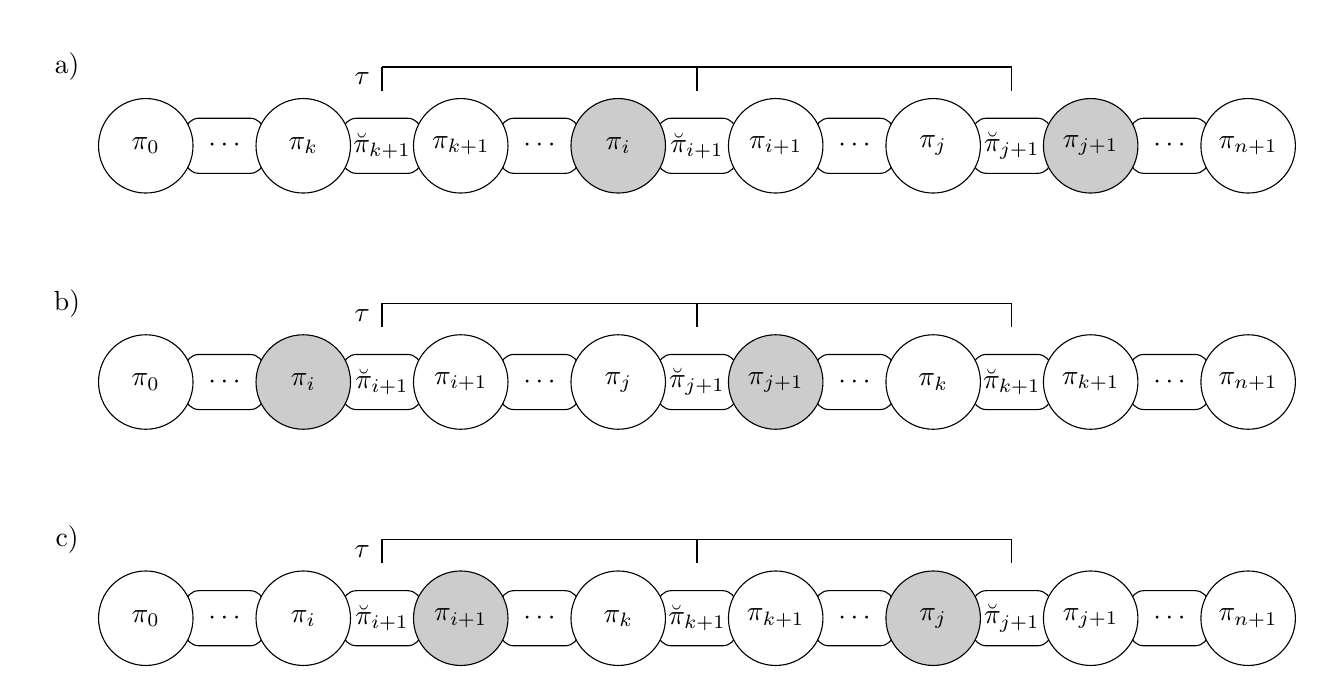
\begin{tikzpicture}
      %%%%% a)

      \node[draw=none,fill=none, minimum height=1cm, minimum width=1cm] at (-3.0, -2.0) {a)};

      % intergenic regions
      \node[rectangle,draw,fill=white!20, minimum height=.7cm, minimum width=1cm, rounded corners=5pt] at (-1.0, -3.0) {$\cdots$};
      \node[rectangle,draw,fill=white!20, minimum height=.7cm, minimum width=1cm, rounded corners=5pt] at (1.0, -3.0) {$\breve\pi_{k+1}$};
      \node[rectangle,draw,fill=white!20, minimum height=.7cm, minimum width=1cm, rounded corners=5pt] at (3.0, -3.0) {$\cdots$};
      \node[rectangle,draw,fill=white!20, minimum height=.7cm, minimum width=1cm, rounded corners=5pt] at (5.0, -3.0) {$\breve\pi_{i+1}$};
      \node[rectangle,draw,fill=white!20, minimum height=.7cm, minimum width=1cm, rounded corners=5pt] at (7.0, -3.0) {$\cdots$};
      \node[rectangle,draw,fill=white!20, minimum height=.7cm, minimum width=1cm, rounded corners=5pt] at (9.0, -3.0) {$\breve\pi_{j+1}$};
      \node[rectangle,draw,fill=white!20, minimum height=.7cm, minimum width=1cm, rounded corners=5pt] at (11.0, -3.0) {$\cdots$};

      % genes
      \node[draw, circle, minimum height=1.2cm, minimum width=1.2cm, fill=white!20] at ({(2*0 - 2)}, -3.0) {$\pi_{0}$};
      \node[draw, circle, minimum height=1.2cm, minimum width=1.2cm, fill=white!20] at ({(2*1 - 2)}, -3.0) {$\pi_{k}$};
      \node[draw, circle, minimum height=1.2cm, minimum width=1.2cm, fill=white!20] at ({(2*2 - 2)}, -3.0) {$\pi_{k+1}$};
      \node[draw, circle, minimum height=1.2cm, minimum width=1.2cm, fill=black!20] at ({(2*3 - 2)}, -3.0) {$\pi_{i}$};
      \node[draw, circle, minimum height=1.2cm, minimum width=1.2cm, fill=white!20] at ({(2*4 - 2)}, -3.0) {$\pi_{i+1}$};
      \node[draw, circle, minimum height=1.2cm, minimum width=1.2cm, fill=white!20] at ({(2*5 - 2)}, -3.0) {$\pi_{j}$};
      \node[draw, circle, minimum height=1.2cm, minimum width=1.2cm, fill=black!20] at ({(2*6 - 2)}, -3.0) {$\pi_{j+1}$};
      \node[draw, circle, minimum height=1.2cm, minimum width=1.2cm, fill=white!20] at ({(2*7 - 2)}, -3.0) {$\pi_{n+1}$};

      % indexes
      \draw (1.0, -2.3) -- (1.0, -2.0);
      \draw (5.0, -2.3) -- (5.0, -2.0);
      \draw (9.0, -2.3) -- (9.0, -2.0);
      \draw (1.0, -2.0) -- (9.0, -2.0);
      \node[draw=none,fill=none] at (0.75, -2.15) {$\tau$};

      %%%%% b)

      \node[draw=none,fill=none, minimum height=1cm, minimum width=1cm] at (-3.0, -5.0) {b)};

      % intergenic regions
      \node[rectangle,draw,fill=white!20, minimum height=.7cm, minimum width=1cm, rounded corners=5pt] at (-1.0, -6.0) {$\cdots$};
      \node[rectangle,draw,fill=white!20, minimum height=.7cm, minimum width=1cm, rounded corners=5pt] at (1.0, -6.0) {$\breve\pi_{i+1}$};
      \node[rectangle,draw,fill=white!20, minimum height=.7cm, minimum width=1cm, rounded corners=5pt] at (3.0, -6.0) {$\cdots$};
      \node[rectangle,draw,fill=white!20, minimum height=.7cm, minimum width=1cm, rounded corners=5pt] at (5.0, -6.0) {$\breve\pi_{j+1}$};
      \node[rectangle,draw,fill=white!20, minimum height=.7cm, minimum width=1cm, rounded corners=5pt] at (7.0, -6.0) {$\cdots$};
      \node[rectangle,draw,fill=white!20, minimum height=.7cm, minimum width=1cm, rounded corners=5pt] at (9.0, -6.0) {$\breve\pi_{k+1}$};
      \node[rectangle,draw,fill=white!20, minimum height=.7cm, minimum width=1cm, rounded corners=5pt] at (11.0, -6.0) {$\cdots$};

      % genes
      \node[draw, circle, minimum height=1.2cm, minimum width=1.2cm, fill=white!20] at ({(2*0 - 2)}, -6.0) {$\pi_{0}$};
      \node[draw, circle, minimum height=1.2cm, minimum width=1.2cm, fill=black!20] at ({(2*1 - 2)}, -6.0) {$\pi_{i}$};
      \node[draw, circle, minimum height=1.2cm, minimum width=1.2cm, fill=white!20] at ({(2*2 - 2)}, -6.0) {$\pi_{i+1}$};
      \node[draw, circle, minimum height=1.2cm, minimum width=1.2cm, fill=white!20] at ({(2*3 - 2)}, -6.0) {$\pi_{j}$};
      \node[draw, circle, minimum height=1.2cm, minimum width=1.2cm, fill=black!20] at ({(2*4 - 2)}, -6.0) {$\pi_{j+1}$};
      \node[draw, circle, minimum height=1.2cm, minimum width=1.2cm, fill=white!20] at ({(2*5 - 2)}, -6.0) {$\pi_{k}$};
      \node[draw, circle, minimum height=1.2cm, minimum width=1.2cm, fill=white!20] at ({(2*6 - 2)}, -6.0) {$\pi_{k+1}$};
      \node[draw, circle, minimum height=1.2cm, minimum width=1.2cm, fill=white!20] at ({(2*7 - 2)}, -6.0) {$\pi_{n+1}$};

      % indexes
      \draw (1.0, -5.3) -- (1.0, -5.0);
      \draw (5.0, -5.3) -- (5.0, -5.0);
      \draw (9.0, -5.3) -- (9.0, -5.0);
      \draw (1.0, -5.0) -- (9.0, -5.0);
      \node[draw=none,fill=none] at (0.75, -5.15) {$\tau$};

      %%%%% c)

      \node[draw=none,fill=none, minimum height=1cm, minimum width=1cm] at (-3.0, -8.0) {c)};

      % intergenic regions
      \node[rectangle,draw,fill=white!20, minimum height=.7cm, minimum width=1cm, rounded corners=5pt] at (-1.0, -9.0) {$\cdots$};
      \node[rectangle,draw,fill=white!20, minimum height=.7cm, minimum width=1cm, rounded corners=5pt] at (1.0, -9.0) {$\breve\pi_{i+1}$};
      \node[rectangle,draw,fill=white!20, minimum height=.7cm, minimum width=1cm, rounded corners=5pt] at (3.0, -9.0) {$\cdots$};
      \node[rectangle,draw,fill=white!20, minimum height=.7cm, minimum width=1cm, rounded corners=5pt] at (5.0, -9.0) {$\breve\pi_{k+1}$};
      \node[rectangle,draw,fill=white!20, minimum height=.7cm, minimum width=1cm, rounded corners=5pt] at (7.0, -9.0) {$\cdots$};
      \node[rectangle,draw,fill=white!20, minimum height=.7cm, minimum width=1cm, rounded corners=5pt] at (9.0, -9.0) {$\breve\pi_{j+1}$};
      \node[rectangle,draw,fill=white!20, minimum height=.7cm, minimum width=1cm, rounded corners=5pt] at (11.0, -9.0) {$\cdots$};

      % genes
      \node[draw, circle, minimum height=1.2cm, minimum width=1.2cm, fill=white!20] at ({(2*0 - 2)}, -9.0) {$\pi_{0}$};
      \node[draw, circle, minimum height=1.2cm, minimum width=1.2cm, fill=white!20] at ({(2*1 - 2)}, -9.0) {$\pi_{i}$};
      \node[draw, circle, minimum height=1.2cm, minimum width=1.2cm, fill=black!20] at ({(2*2 - 2)}, -9.0) {$\pi_{i+1}$};
      \node[draw, circle, minimum height=1.2cm, minimum width=1.2cm, fill=white!20] at ({(2*3 - 2)}, -9.0) {$\pi_{k}$};
      \node[draw, circle, minimum height=1.2cm, minimum width=1.2cm, fill=white!20] at ({(2*4 - 2)}, -9.0) {$\pi_{k+1}$};
      \node[draw, circle, minimum height=1.2cm, minimum width=1.2cm, fill=black!20] at ({(2*5 - 2)}, -9.0) {$\pi_{j}$};
      \node[draw, circle, minimum height=1.2cm, minimum width=1.2cm, fill=white!20] at ({(2*6 - 2)}, -9.0) {$\pi_{j+1}$};
      \node[draw, circle, minimum height=1.2cm, minimum width=1.2cm, fill=white!20] at ({(2*7 - 2)}, -9.0) {$\pi_{n+1}$};

      % indexes
      \draw (1.0, -8.3) -- (1.0, -8.0);
      \draw (5.0, -8.3) -- (5.0, -8.0);
      \draw (9.0, -8.3) -- (9.0, -8.0);
      \draw (1.0, -8.0) -- (9.0, -8.0);
      \node[draw=none,fill=none] at (0.75, -8.15) {$\tau$};
    \end{tikzpicture}
  }
  \caption[Exemplo de remoção de, pelo menos, um breakpoint tipo um após a aplicação de uma transposição $\tau$.]{Exemplo de remoção de, pelo menos, um breakpoint tipo um após a aplicação de uma transposição $\tau$.}
  \label{figure:WDJFPAXN}
\end{figure}

Considere o Algoritmo~\ref{algorithm:SAAUGXYG} para a variação sem sinais do problema \SbIRT{}.

\begin{algorithm}[!tbh]
  \caption{Um algoritmo de aproximação para o problema \SbIR{}.\label{algorithm:SAAUGXYG}}
  \Entrada{Uma instância intergênica rígida balanceada sem sinais $\mathcal{I}=((\pi,\breve\pi),(\iota,\breve\iota))$}
  \Saida{Uma sequência de reversões e transposições $S$, tal que $(\pi,\breve\pi) \cdot S = (\iota,\breve\iota)$}
    Seja $S \gets ()$ \\
    \Enqto{$ib(\mathcal{I}) > 1$}{
      \tcp{Lema~\ref{lemma:WYEZMYTM}}
      $(\pi_i,\pi_{i+1})$, $(\pi_j,\pi_{j+1}) \gets $ encontre um par de breakpoints conectados \\
      \tcp{Lema~\ref{lemma:SIAFJFDO}}
      \Se{$(\pi_i,\pi_{i+1})$, $(\pi_j,\pi_{j+1})$ pertence ao caso $i$}{
        $S' \gets (\rho_1)$ \\
      }\SenaoSe{$(\pi_i,\pi_{i+1})$, $(\pi_j,\pi_{j+1})$ pertence ao caso $ii$}{
        $S' \gets (\tau_1)$ \\
      }\SenaoSe{$(\pi_i,\pi_{i+1})$, $(\pi_j,\pi_{j+1})$ pertence ao caso $iii$}{
        $S' \gets (\tau_1)$ \\
      }\SenaoSe{$(\pi_i,\pi_{i+1})$, $(\pi_j,\pi_{j+1})$ pertence ao caso $iv$}{
        $S' \gets (\rho_1,\rho_2)$ \\
      }
      $S \gets S + S'$ \\
      $\mathcal{I} \gets ((\pi, \breve\pi) \cdot S',(\iota,\breve\iota))$ \\
    }
  \Retorna{S}
\end{algorithm}

\begin{lemma}\label{lemma:QMLCZMMK}
Seja $\mathcal{I} = ((\pi,\breve\pi),(\iota,\breve\iota))$ uma instância intergênica rígida balanceada sem sinais. O Algoritmo~\ref{algorithm:SAAUGXYG} transforma $(\pi,\breve\pi)$ em $(\iota,\breve\iota)$ utilizando, no máximo, $2ib_1(\mathcal{I})$ eventos de reversão e transposição.
\end{lemma}
\begin{proof}
  No Algoritmo~\ref{algorithm:SAAUGXYG}, temos que enquanto $ib_1(\mathcal{I})$ for maior que um, ou seja, $(\pi,\breve\pi)$ for diferente de $(\iota,\breve\iota)$ (pela Observação~\ref{remark:UDYJTHAH} e Lema~\ref{lemma:WSPRPLAH}), o seguinte procedimento é aplicado: pelos lemas~\ref{lemma:WYEZMYTM} e~\ref{lemma:SIAFJFDO}, sempre podemos encontrar um par conectado de breakpoints e remover pelo menos um breakpoint tipo um após aplicar, no máximo, duas reversões ou uma transposição. A cada iteração do algoritmo, pelo menos um breakpoint tipo um é removido. Dessa forma, o genoma alvo eventualmente será alcançado. No pior caso, cada breakpoint tipo um é removido utilizando dois eventos de rearranjo. Logo, uma sequência com, no máximo, $2ib_1(\mathcal{I})$ reversões e transposições é utilizada para transformar $(\pi,\breve\pi)$ em $(\iota,\breve\iota)$ e o lema segue.
\end{proof}

Note que o Algoritmo~\ref{algorithm:SAAUGXYG}, em comparação com o Algoritmo~\ref{algorithm:AKKUXQNR}, difere apenas pelos casos $(ii)$ e $(iii)$ de um par conectado de breakpoints, que também podem ser realizados em tempo linear. Logo, o tempo de execução do Algoritmo~\ref{algorithm:SAAUGXYG} também é $\mathcal{O}(n^2)$.

\begin{theorem}\label{theorem:ZEFRNBIE}
O Algoritmo~\ref{algorithm:SAAUGXYG} é uma $6$-aproximação para a variação sem sinais do problema \SbIRT{}.
\end{theorem}
\begin{proof}
Seja $\mathcal{I} = ((\pi,\breve\pi),(\iota,\breve\iota))$ uma instância intergênica rígida balanceada sem sinais. Pelo Lema~\ref{lemma:QMLCZMMK}, o Algoritmo~\ref{algorithm:SAAUGXYG} transforma $(\pi,\breve\pi)$ em $(\iota,\breve\iota)$ utilizando, no máximo, $2ib_1(\mathcal{I})$ eventos de reversão e transposição. Pelo Teorema~\ref{theorem:MPFPKHQO}, temos o seguinte limitante inferior: $di_{\RT}(\mathcal{I}) \ge \frac{ib_1(\mathcal{I})}{3}$. Logo, o teorema segue. 
\end{proof}

A seguir, apresentaremos lemas que serão utilizados para obtermos um algoritmo de aproximação com fator $4.5$ para a variação sem sinais do problema \SbIRT{}.

\begin{lemma}\label{lemma:RAJPFOWJ}
Seja $(\pi,\breve\pi)$ uma representação intergênica rígida e sejam duas transposições consecutivas no formato $\tau^{(i,j,k)}_{(\varphi_i,\varphi_j,\varphi_k)}$ e $\tau^{(i,i+k-j,k)}_{(\varphi^\prime_i,\varphi^\prime_{i+k-j},\varphi^\prime_k)}$. É possível realizar qualquer redistribuição de nucleotídeos nas regiões intergênicas $\breve\pi_i$, $\breve\pi_j$ e $\breve\pi_k$ após aplicas consecutivamente as transposições $\tau^{(i,j,k)}_{(\varphi_i,\varphi_j,\varphi_k)}$ e $\tau^{(i,i+k-j,k)}_{(\varphi^\prime_i,\varphi^\prime_{i+k-j},\varphi^\prime_k)}$ em $(\pi,\breve\pi)$.
\end{lemma} 
\begin{proof}
Temos que mostrar que sempre é possível encontrar valores para as triplas $(\varphi_i,\varphi_j,\varphi_k)$ e $(\varphi^\prime_i,\varphi^\prime_{i+k-j},\varphi^\prime_k)$ para qualquer redistribuição de nucleotídeos nas regiões intergênicas $\breve\pi_i$, $\breve\pi_j$ e $\breve\pi_k$.

Como usamos apenas transposições, sabemos que $\breve\pi_i + \breve\pi_j + \breve\pi_k = \breve\pi^{\prime\prime}_i + \breve\pi^{\prime\prime}_j + \breve\pi^{\prime\prime}_k$, onde $\breve\pi^{\prime\prime}_i$, $\breve\pi^{\prime\prime}_j$ e $\breve \pi^{\prime\prime}_k$ representam os tamanhos das regiões intergênicas após a aplicação das duas transposições consecutivas.

Com base no fluxo de nucleotídeos entre as regiões intergênicas, realizaremos uma redução para uma instância $I_{MF}$ do problema de fluxo máximo, e mostraremos que sempre é possível encontrar uma solução para essa instância que satisfaça as restrições de redistribuição das regiões intergênicas $\breve\pi_i$, $\breve\pi_j$ e $\breve\pi_k$. Uma instância do problema de fluxo máximo é dada em um grafo onde cada aresta possui uma capacidade máxima de fluxo que pode ser transferido entre o par de vértices conectados. O objetivo consiste em determinar o fluxo máximo que pode ser enviado de um vértice de origem até um vértice de destino no grafo.

A Figura~\ref{figure:XUQWDNIW} (esquerda) mostra o fluxo que os nucleotídeos nas regiões intergênicas podem seguir ao aplicar as duas transposições consecutivas (declaradas no enunciado). Note que cada região intergênica pode enviar nucleotídeos para duas regiões intergênicas distintas. Assim, podemos criar um grafo, com vértices numerados de 1 até 9, onde cada vértice corresponde a uma região intergênica e onde existe um arco $(f,g)$ com capacidade ilimitada se a região intergênica $f$ puder enviar nucleotídeos para a região intergênica $g$.

Por fim, para obter a instância $I_{MF}$ do problema de fluxo máximo, adicionaremos os vértices 0 (origem) e 10 (destino), juntamente com os seguintes arcos: $(0,1)$, $(0, 2)$, $(0,3)$, $(7,10)$, $(8,10)$ e $(9,10)$ com suas respectivas capacidades: $a=\breve\pi_i$, $b=\breve\pi_j$, $c=\breve\pi_k$, $x=\breve\pi^{\prime\prime}_i$, $y=\breve\pi^{\prime\prime}_j $ e $z=\breve\pi^{\prime\prime}_k$. Todos os outros arcos têm capacidade infinita atribuída. A Figura~\ref{figure:XUQWDNIW} (direita) mostra a instância $I_{MF}$ obtida do problema de fluxo máximo.

\begin{figure}[!tbh]
  \resizebox{.45\linewidth}{!}{
    \centering  
    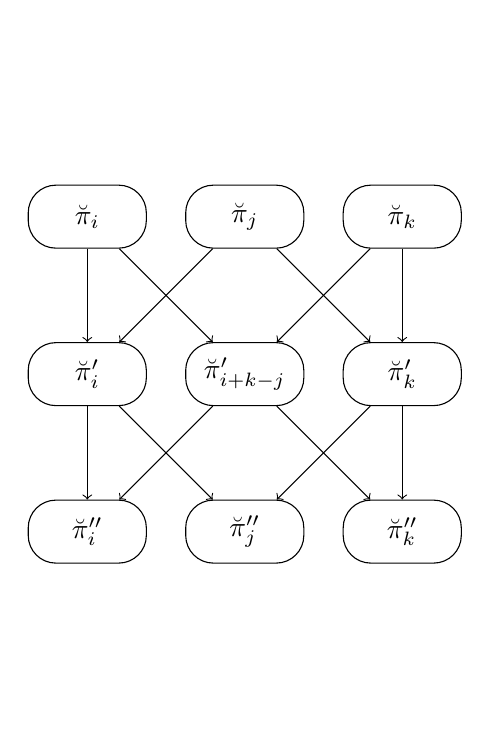
\begin{tikzpicture}
      \tikzstyle{STY1} = [draw, rectangle, minimum height=.8cm, minimum width=1.5cm, rounded corners=10pt]
      \tikzstyle{STY2} = [->]

      %%%%% VERTEX

      \node[draw=none, fill=none, rectangle, minimum height=.8cm, minimum width=1.5cm, rounded corners=10pt](v0) at ({(2*2 - 2)}, 2.0) {};

      \node[STY1](v1) at ({(2*1 - 2)}, 0.0) {$\breve\pi_i$};
      \node[STY1](v2) at ({(2*2 - 2)}, 0.0) {$\breve\pi_j$};
      \node[STY1](v3) at ({(2*3 - 2)}, 0.0) {$\breve\pi_k$};

      \node[STY1](v4) at ({(2*1 - 2)}, -2.0) {$\breve\pi^{\prime}_i$};
      \node[STY1](v5) at ({(2*2 - 2)}, -2.0) {$\breve\pi^{\prime}_{i+k-j}$};
      \node[STY1](v6) at ({(2*3 - 2)}, -2.0) {$\breve\pi^{\prime}_k$};


      \node[STY1](v7) at ({(2*1 - 2)}, -4.0) {$\breve\pi^{\prime\prime}_i$};
      \node[STY1](v8) at ({(2*2 - 2)}, -4.0) {$\breve\pi^{\prime\prime}_j$};
      \node[STY1](v9) at ({(2*3 - 2)}, -4.0) {$\breve\pi^{\prime\prime}_k$};

      \node[draw=none, fill=none, rectangle, minimum height=.8cm, minimum width=1.5cm, rounded corners=10pt](v10) at ({(2*2 - 2)}, -6.0) {};

      %%%%% EDGES

      \draw[STY2]  (v1) edge (v4);
      \draw[STY2]  (v1) edge (v5);
      \draw[STY2]  (v2) edge (v4);
      \draw[STY2]  (v2) edge (v6);
      \draw[STY2]  (v3) edge (v5);
      \draw[STY2]  (v3) edge (v6);

      \draw[STY2]  (v4) edge (v7);
      \draw[STY2]  (v4) edge (v8);
      \draw[STY2]  (v5) edge (v7);
      \draw[STY2]  (v5) edge (v9);
      \draw[STY2]  (v6) edge (v8);
      \draw[STY2]  (v6) edge (v9);
      %     \node[draw=none,fill=none, minimum height=1cm, minimum width=1cm] at (0.0, 2.0) {a)};
    \end{tikzpicture}
  }
  \hfill
  \resizebox{.45\linewidth}{!}{
    \centering
    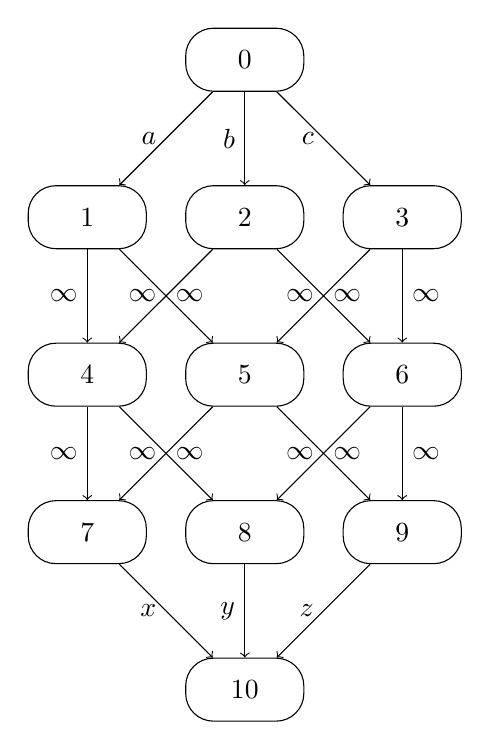
\begin{tikzpicture}
      \tikzstyle{STY1} = [draw, rectangle, minimum height=.8cm, minimum width=1.5cm, rounded corners=10pt]
      \tikzstyle{STY2} = [->]

      %%%%% VERTEX

      \node[STY1](v0) at ({(2*2 - 2)}, 2.0) {0};

      \node[STY1](v1) at ({(2*1 - 2)}, 0.0) {1};
      \node[STY1](v2) at ({(2*2 - 2)}, 0.0) {2};
      \node[STY1](v3) at ({(2*3 - 2)}, 0.0) {3};

      \node[STY1](v4) at ({(2*1 - 2)}, -2.0) {4};
      \node[STY1](v5) at ({(2*2 - 2)}, -2.0) {5};
      \node[STY1](v6) at ({(2*3 - 2)}, -2.0) {6};


      \node[STY1](v7) at ({(2*1 - 2)}, -4.0) {7};
      \node[STY1](v8) at ({(2*2 - 2)}, -4.0) {8};
      \node[STY1](v9) at ({(2*3 - 2)}, -4.0) {9};

      \node[STY1](v10) at ({(2*2 - 2)}, -6.0) {10};

      %%%%% EDGES
      \draw[STY2]  (v0) edge node[anchor=center, left, midway] {$a$} (v1);
      \draw[STY2]  (v0) edge node[anchor=center, left, midway] {$b$} (v2);
      \draw[STY2]  (v0) edge node[anchor=center, left, midway] {$c$} (v3);

      \draw[STY2]  (v1) edge node[anchor=center, left, midway] {$\infty$} (v4);
      \draw[STY2]  (v1) edge node[anchor=center, left, midway] {$\infty$} (v5);
      \draw[STY2]  (v2) edge node[anchor=center, right, midway] {$\infty$} (v4);
      \draw[STY2]  (v2) edge node[anchor=center, left, midway] {$\infty$} (v6);
      \draw[STY2]  (v3) edge node[anchor=center, right, midway] {$\infty$} (v5);
      \draw[STY2]  (v3) edge node[anchor=center, right, midway] {$\infty$} (v6);

      \draw[STY2]  (v4) edge node[anchor=center, left, midway] {$\infty$} (v7);
      \draw[STY2]  (v4) edge node[anchor=center, left, midway] {$\infty$} (v8);
      \draw[STY2]  (v5) edge node[anchor=center, right, midway] {$\infty$} (v7);
      \draw[STY2]  (v5) edge node[anchor=center, left, midway] {$\infty$} (v9);
      \draw[STY2]  (v6) edge node[anchor=center, right, midway] {$\infty$} (v8);
      \draw[STY2]  (v6) edge node[anchor=center, right, midway] {$\infty$} (v9);

      \draw[STY2]  (v7) edge node[anchor=center, left, midway] {$x$} (v10);
      \draw[STY2]  (v8) edge node[anchor=center, left, midway] {$y$} (v10);
      \draw[STY2]  (v9) edge node[anchor=center, left, midway] {$z$} (v10);

      %     \node[draw=none,fill=none, minimum height=1cm, minimum width=1cm] at (0.0, 2.0) {b)};
    \end{tikzpicture}
  }
  \caption[Exemplo de fluxo de nucleotídeos entre as regiões intergênicas.]{No lado esquerdo, uma representação do fluxo de nucleotídeos entre as regiões intergênicas. No lado direito, a instância $I_{MF}$ do problema de fluxo máximo com os vértices de origem (0) e destino (10).}
  \label{figure:XUQWDNIW}
\end{figure}

Se analisarmos a Figura~\ref{figure:XUQWDNIW} (direita), podemos ver que o fluxo máximo da instância $I_{MF}$ é limitado a $\max\{(a+b+c),(x+ y+z)\}$, mas sabemos que $(a+b+c) = (x+y+z) = F$. Observe também que, se houver uma redistribuição das regiões intergênicas $\breve\pi_i$, $\breve\pi_j$ e $\breve\pi_k$, isso significa que a instância $I_{MF}$ tem uma solução onde o máximo fluxo é $F$. Por outro lado, podemos ver que, se a instância $I_{MF}$ tiver uma solução com fluxo máximo de $F$ e todas as variáveis da solução forem inteiras, isso significa que é possível redistribuir as regiões intergênicas $\breve \pi_i$, $\breve\pi_j$ e $\breve\pi_k$.

Agora, mostraremos que a instância $I_{MF}$ sempre tem uma solução com fluxo máximo $F$, onde todas as variáveis da solução são inteiras. Vamos provar este resultado fornecendo uma solução para a instância $I_{MF}$, que é obtida em três etapas.

A etapa 1 consiste em remover os vértices 8 e 9 de $I_{MF}$ (Figura~\ref{figure:NCRGBSMG} (esquerda)), e resolver a instância usando Programação Linear (PL) para obter uma possível solução fracionária. Observe que o fluxo máximo para essa etapa é menor ou igual a $x$, pois $(a+b+c) \ge x$ e $x$ é o valor do corte mínimo para a instância. Além disso, existe uma solução que atinge exatamente $x$ (por exemplo, envie até $a$ pelo caminho $(1,4,7)$; envie até $b$ pelo caminho $(2,4,7)$; envie até $c$ pelo caminho $(3,5,7)$). Seja $X^{\prime}$ a matriz da solução, na qual $X^{\prime}_{i,j}$ representa o fluxo que vai do vértice $i$ ao vértice $j$ na solução. Sabemos que $(X^{\prime}_{0,1}+X^{\prime}_{0,2}+X^{\prime}_{0,3}) = x$ e $x \in \mathbb{N}$. Se $\{X^{\prime}_{0,1},X^{\prime}_{0,2},X^{\prime}_{0,3}\} \not\subset \mathbb {N}$, podemos obter valores inteiros para as variáveis $X^{\prime}_{0,1}$, $X^{\prime}_{0,2}$ e $X^{\prime }_{0,3}$ redistribuindo a parte fracionária entre os arcos, isso é possível porque sabemos que $(a+b+c) \ge x$. Como todos os caminhos que partem dos vértices 1, 2 e 3 e chegam ao vértice 7 têm capacidade ilimitada, podemos obter uma solução inteira para as variáveis restantes. Após esse processo, obtemos uma solução inteira $X^{\prime}$ para a etapa 1.

A etapa 2 consiste em remover os vértices 7 e 9 de $I_{MF}$, e atualizar a capacidade dos arcos $(0,1)$, $(0,2)$ e $(0,3)$ para $a ^{\prime}=a-X^{\prime}_{0,1}$, $b^{\prime}=b-X^{\prime}_{0,2}$ e $c^{\prime} =c-X^{\prime}_{0,3}$, respectivamente (Figura~\ref{figure:NCRGBSMG} (centro)). Em outras palavras, levamos em consideração, para os arcos $(0,1)$, $(0,2)$ e $(0,3)$, as capacidades que já foram utilizadas na etapa 1. Observe que $a^{\prime}+b^{\prime}+c^{\prime} = a+b+c-x$, mas também sabemos que $a+b+c = x+y+z$, assim $a^{\prime}+b^{\prime}+c^{\prime} = a+b+c-x = y+z \geq y$. Observe que o fluxo máximo para essa etapa é menor ou igual a $y$, pois $a^{\prime}+b^{\prime}+c^{\prime} \ge y$ e $y$ é o valor do corte mínimo para a instância. Além disso, existe uma solução que atinge exatamente $y$ (por exemplo, envie até $a^{\prime}$ pelo caminho $(1,4,8)$; envie até $b^{\prime}$ pelo caminho $(2,4,8) $; envie até $c^{\prime}$ pelo caminho $(3,6,8)$). Similarmente ao processo realizado na etapa 1, resolvemos o problema para obter uma solução $X^{\prime\prime}$ onde o fluxo máximo é $y$ e todas as variáveis são inteiras.

A etapa 3 consiste em remover os vértices 7 e 8 de $I_{MF}$, e atualizar a capacidade dos arcos $(0,1)$, $(0,2)$ e $(0,3)$ para $a ^{\prime\prime}=a^{\prime}-X^{\prime\prime}_{0,1}$, $b^{\prime\prime}=b^{\prime}-X^ {\prime\prime}_{0,2}$ e $c^{\prime\prime}=c^{\prime}-X^{\prime\prime}_{0,3}$, respectivamente (Figura~\ref{figure:NCRGBSMG} (direita)). Em outras palavras, levamos em consideração, para os arcos $(0,1)$, $(0,2)$ e $(0,3)$, as capacidades que já foram utilizadas nas etapas~1 e~2. Observe que $a^{\prime\prime}+b^{\prime\prime}+c^{\prime\prime} = a+b+c-x-y$, mas também sabemos que $a+b+c = x +y+z$, portanto $a^{\prime\prime}+b^{\prime\prime}+c^{\prime\prime} = a+b+c-x-y = z$. Observe que o fluxo máximo para essa etapa é igual a $z$, pois $a^{\prime\prime}+b^{\prime\prime}+c^{\prime\prime} = z$, e existe uma solução que atinge exatamente $z$ (por exemplo, envie $a^{\prime\prime}$ pelo caminho $(1,5,9)$; envie $b^{\prime\prime}$ pelo caminho $ (2,6,9)$; envie $c^{\prime\prime}$ pelo caminho $(3,6,9)$). Da mesma forma que o processo realizado na etapa 1, resolvemos o problema para obter uma solução $X^{\prime\prime\prime}$ onde o fluxo máximo é $z$ e todas as variáveis são números inteiros.

\begin{figure}[!tbh]
  \resizebox{.3\linewidth}{!}{
    \centering
    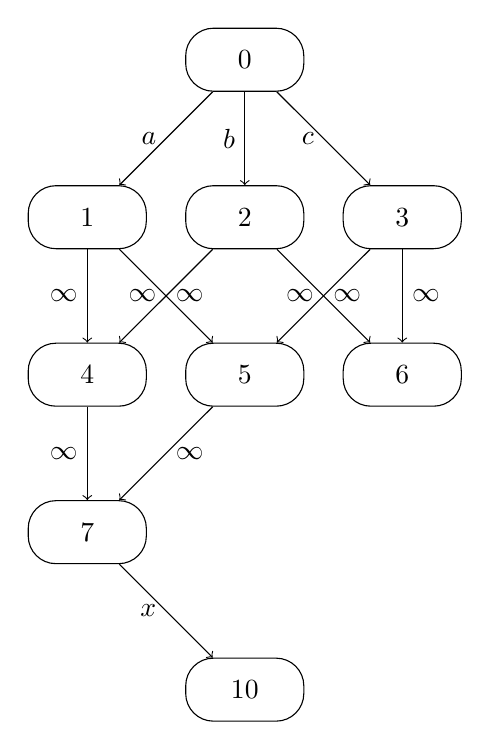
\begin{tikzpicture}
      \tikzstyle{STY1} = [draw, rectangle, minimum height=.8cm, minimum width=1.5cm, rounded corners=10pt]
      \tikzstyle{STY2} = [->]

      %%%%% VERTEX

      \node[STY1](v0) at ({(2*2 - 2)}, 2.0) {0};

      \node[STY1](v1) at ({(2*1 - 2)}, 0.0) {1};
      \node[STY1](v2) at ({(2*2 - 2)}, 0.0) {2};
      \node[STY1](v3) at ({(2*3 - 2)}, 0.0) {3};

      \node[STY1](v4) at ({(2*1 - 2)}, -2.0) {4};
      \node[STY1](v5) at ({(2*2 - 2)}, -2.0) {5};
      \node[STY1](v6) at ({(2*3 - 2)}, -2.0) {6};


      \node[STY1](v7) at ({(2*1 - 2)}, -4.0) {7};

      \node[STY1](v10) at ({(2*2 - 2)}, -6.0) {10};

      %%%%% EDGES
      \draw[STY2]  (v0) edge node[anchor=center, left, midway] {$a$} (v1);
      \draw[STY2]  (v0) edge node[anchor=center, left, midway] {$b$} (v2);
      \draw[STY2]  (v0) edge node[anchor=center, left, midway] {$c$} (v3);

      \draw[STY2]  (v1) edge node[anchor=center, left, midway] {$\infty$} (v4);
      \draw[STY2]  (v1) edge node[anchor=center, left, midway] {$\infty$} (v5);
      \draw[STY2]  (v2) edge node[anchor=center, right, midway] {$\infty$} (v4);
      \draw[STY2]  (v2) edge node[anchor=center, left, midway] {$\infty$} (v6);
      \draw[STY2]  (v3) edge node[anchor=center, right, midway] {$\infty$} (v5);
      \draw[STY2]  (v3) edge node[anchor=center, right, midway] {$\infty$} (v6);

      \draw[STY2]  (v4) edge node[anchor=center, left, midway] {$\infty$} (v7);
      \draw[STY2]  (v5) edge node[anchor=center, right, midway] {$\infty$} (v7);

      \draw[STY2]  (v7) edge node[anchor=center, left, midway] {$x$} (v10);

      %     \node[draw=none,fill=none, minimum height=1cm, minimum width=1cm] at (0.0, 2.0) {a)};
    \end{tikzpicture}
  }
  \hfill
  \resizebox{.3\linewidth}{!}{
    \centering
    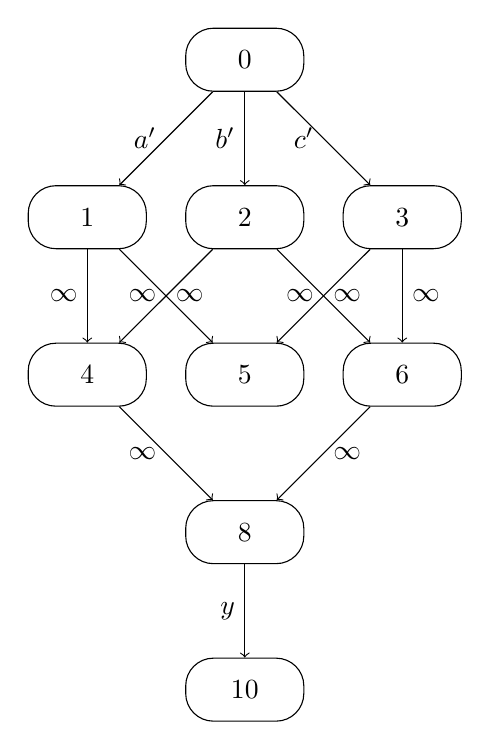
\begin{tikzpicture}
      \tikzstyle{STY1} = [draw, rectangle, minimum height=.8cm, minimum width=1.5cm, rounded corners=10pt]
      \tikzstyle{STY2} = [->]

      %%%%% VERTEX

      \node[STY1](v0) at ({(2*2 - 2)}, 2.0) {0};

      \node[STY1](v1) at ({(2*1 - 2)}, 0.0) {1};
      \node[STY1](v2) at ({(2*2 - 2)}, 0.0) {2};
      \node[STY1](v3) at ({(2*3 - 2)}, 0.0) {3};

      \node[STY1](v4) at ({(2*1 - 2)}, -2.0) {4};
      \node[STY1](v5) at ({(2*2 - 2)}, -2.0) {5};
      \node[STY1](v6) at ({(2*3 - 2)}, -2.0) {6};

      \node[STY1](v8) at ({(2*2 - 2)}, -4.0) {8};

      \node[STY1](v10) at ({(2*2 - 2)}, -6.0) {10};

      %%%%% EDGES
      \draw[STY2]  (v0) edge node[anchor=center, left, midway] {$a^{\prime}$} (v1);
      \draw[STY2]  (v0) edge node[anchor=center, left, midway] {$b^{\prime}$} (v2);
      \draw[STY2]  (v0) edge node[anchor=center, left, midway] {$c^{\prime}$} (v3);

      \draw[STY2]  (v1) edge node[anchor=center, left, midway] {$\infty$} (v4);
      \draw[STY2]  (v1) edge node[anchor=center, left, midway] {$\infty$} (v5);
      \draw[STY2]  (v2) edge node[anchor=center, right, midway] {$\infty$} (v4);
      \draw[STY2]  (v2) edge node[anchor=center, left, midway] {$\infty$} (v6);
      \draw[STY2]  (v3) edge node[anchor=center, right, midway] {$\infty$} (v5);
      \draw[STY2]  (v3) edge node[anchor=center, right, midway] {$\infty$} (v6);

      \draw[STY2]  (v4) edge node[anchor=center, left, midway] {$\infty$} (v8);
      \draw[STY2]  (v6) edge node[anchor=center, right, midway] {$\infty$} (v8);
      \draw[STY2]  (v8) edge node[anchor=center, left, midway] {$y$} (v10);

      %     \node[draw=none,fill=none, minimum height=1cm, minimum width=1cm] at (0.0, 2.0) {b)};
    \end{tikzpicture}
  }
  \hfill
  \resizebox{.3\linewidth}{!}{
    \centering
    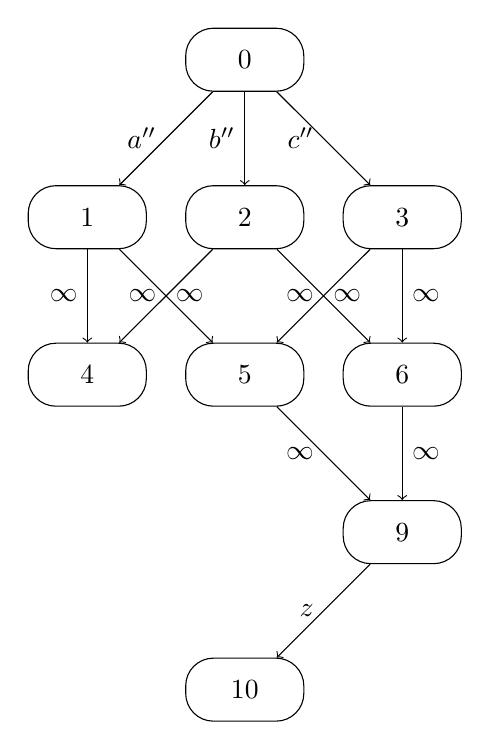
\begin{tikzpicture}
      \tikzstyle{STY1} = [draw, rectangle, minimum height=.8cm, minimum width=1.5cm, rounded corners=10pt]
      \tikzstyle{STY2} = [->]

      %%%%% VERTEX

      \node[STY1](v0) at ({(2*2 - 2)}, 2.0) {0};

      \node[STY1](v1) at ({(2*1 - 2)}, 0.0) {1};
      \node[STY1](v2) at ({(2*2 - 2)}, 0.0) {2};
      \node[STY1](v3) at ({(2*3 - 2)}, 0.0) {3};

      \node[STY1](v4) at ({(2*1 - 2)}, -2.0) {4};
      \node[STY1](v5) at ({(2*2 - 2)}, -2.0) {5};
      \node[STY1](v6) at ({(2*3 - 2)}, -2.0) {6};

      \node[STY1](v9) at ({(2*3 - 2)}, -4.0) {9};

      \node[STY1](v10) at ({(2*2 - 2)}, -6.0) {10};

      %%%%% EDGES
      \draw[STY2]  (v0) edge node[anchor=center, left, midway] {$a^{\prime\prime}$} (v1);
      \draw[STY2]  (v0) edge node[anchor=center, left, midway] {$b^{\prime\prime}$} (v2);
      \draw[STY2]  (v0) edge node[anchor=center, left, midway] {$c^{\prime\prime}$} (v3);

      \draw[STY2]  (v1) edge node[anchor=center, left, midway] {$\infty$} (v4);
      \draw[STY2]  (v1) edge node[anchor=center, left, midway] {$\infty$} (v5);
      \draw[STY2]  (v2) edge node[anchor=center, right, midway] {$\infty$} (v4);
      \draw[STY2]  (v2) edge node[anchor=center, left, midway] {$\infty$} (v6);
      \draw[STY2]  (v3) edge node[anchor=center, right, midway] {$\infty$} (v5);
      \draw[STY2]  (v3) edge node[anchor=center, right, midway] {$\infty$} (v6);

      \draw[STY2]  (v5) edge node[anchor=center, left, midway] {$\infty$} (v9);
      \draw[STY2]  (v6) edge node[anchor=center, right, midway] {$\infty$} (v9);
      \draw[STY2]  (v9) edge node[anchor=center, left, midway] {$z$} (v10);

      %     \node[draw=none,fill=none, minimum height=1cm, minimum width=1cm] at (0.0, 2.0) {c)};
    \end{tikzpicture}
  }
  \caption[Divisão da instância $I_{MF}$ do problema de fluxo máximo em três etapas.]{Divisão da instância $I_{MF}$ do problema de fluxo máximo em três etapas.}
  \label{figure:NCRGBSMG}
\end{figure}

A solução final $X$ consiste na soma de todas as capacidades utilizadas pelas soluções nas etapas 1, 2 e 3, ou seja, $\forall$~$1\leq i,j\leq 10$, $X_{i, j} = X^{\prime}_{i,j} + X^{\prime\prime}_{i,j} + X^{\prime\prime\prime}_{i,j}$. Observe que a solução $X$ não viola nenhuma restrição de capacidade, todas as variáveis são inteiras e o fluxo máximo é $F=a+b+c=x+y+z$.

\end{proof}

Em resumo, o Lema~\ref{lemma:RAJPFOWJ} nos permite, com duas transposições consecutivas, redistribuir o tamanho de três regiões intergênicas mantendo os genes na mesma ordem e orientação.

\begin{lemma}\label{lemma:FSGHLWJU}
Seja $\mathcal{I} = ((\pi,\breve\pi),(\iota,\breve\iota))$ uma instância intergênica rígida balanceada sem sinais com pelo menos dois breakpoints sobrecarregados. Existe uma sequência de duas transposições que remove pelo menos dois breakpoints tipo um de $\mathcal{I}$.
\end{lemma}
\begin{proof}
Sejam $(\pi_i,\pi_{i+1})$ e $(\pi_j,\pi_{j+1})$ dois breakpoints sobrecarregados de $\mathcal{I}$.
Agora, observe que deve existir um terceiro breakpoint tipo um $(\pi_k,\pi_{k+1})$ em $\mathcal{I}$. Caso contrário, $\mathcal{I}$ seria uma instância desbalanceada. Pelo Lema~\ref{lemma:RAJPFOWJ}, sabemos que é possível realizar qualquer redistribuição de nucleotídeos em três regiões intergênicas utilizando duas transposições consecutivas. Dessa forma, podemos realizar a redistribuição do tamanho das regiões intergênicas $\breve\pi_{i+1}$, $\breve\pi_{j+1}$ e $\breve\pi_{k+1}$ para $\breve\iota_{\max(\pi_i,\pi_{i+1})}$, $\breve\iota_{\max(\pi_j,\pi_{j+1})}$ e $\breve\pi_{k+1} + (\breve\pi_{i+1} - \breve\iota_{\max(\pi_i,\pi_{i+1})}) + (\breve\pi_{j+1} - \breve\iota_{\max(\pi_j,\pi_{j+1})})$, respectivamente. Nesse caso, o excesso de nucleotídeos nos breakpoints sobrecarregados é transferido para o breakpoint $(\pi_k,\pi_{k+1})$. Como resultado, pelo menos dois breakpoints tipo um são removidos após a aplicação de duas transposições, e o lema segue.
\end{proof}

\begin{lemma}\label{lemma:RHTVEKOL}
Seja $\mathcal{I} = ((\pi,\breve\pi),(\iota,\breve\iota))$ uma instância intergênica rígida balanceada sem sinais com apenas um breakpoint sobrecarregado $(\pi_i,\pi_{i+1})$ e com pelo menos um breakpoint subcarregado $(\pi_j,\pi_{j+1})$ tal que $\breve\pi_{i+1} + \breve\pi_{j+1} \ge \breve\iota_{x} + \breve\iota_{y}$, onde $x = \max(\pi_i,\pi_{i+1})$ e $y=\max(\pi_j,\pi_{j+1})$. Existe uma sequência de duas transposições ou duas reversões que remove pelo menos dois breakpoints tipo um de $\mathcal{I}$.
\end{lemma}
\begin{proof}
Note que o excesso de nucleotídeos na região intergênica $\breve\pi_{i+1}$ é maior ou igual à quantidade de nucleotídeos que falta na região intergênica $\breve\pi_{j+1}$. Caso $ib_1(\mathcal{I})\ge 3$, utilizaremos, para selecionar o terceiro breakpoint tipo um $(\pi_k,\pi_{k+1})$ ($k \notin \{i,j\}$), a seguinte ordem de prioridade: breakpoint suave, breakpoint sobrecarregado e breakpoint subcarregado. Note que o terceiro breakpoint tipo um deve ser de um dos tipos da lista de prioridades, obrigatoriamente. Em seguida, aplicamos o mesmo processo descrito no Lema~\ref{lemma:FSGHLWJU}. Caso contrário ($ib_1(\mathcal{I}) < 3$), isso implica que o excesso de nucleotídeos na região intergênica $\breve\pi_{i+1}$ é justamente a quantidade de nucleotídeos que falta na região intergênica $\breve\pi_{j+1}$. Logo, podemos aplicar as duas reversões descritas no caso $iv$ do Lema~\ref{lemma:IMYFBWDY}, e o lema segue.
\end{proof}

\begin{lemma}\label{lemma:ICDGSTEE}
Seja $\mathcal{I} = ((\pi,\breve\pi),(\iota,\breve\iota))$ uma instância intergênica rígida balanceada sem sinais com apenas um breakpoint sobrecarregado $(\pi_i,\pi_{i+1})$ e sem nenhum breakpoint subcarregado $(\pi_j,\pi_{j+1})$ tal que $\breve\pi_{i+1} + \breve\pi_{j+1} \ge \breve\iota_{x} + \breve\iota_{y}$, onde $x = \max(\pi_i,\pi_{i+1})$ e $y=\max(\pi_j,\pi_{j+1})$. Existe uma sequência de duas reversões que remove o breakpoint sobrecarregado $(\pi_i,\pi_{i+1})$ de $\mathcal{I}$ e não gera nenhum outro.
\end{lemma}
\begin{proof}
Note que um breakpoint sobrecarregado sempre vai estar conectado com qualquer outro breakpoint tipo um. Além disso, um segundo breakpoint tipo um $(\pi_k,\pi_{k+1})$ deve existir (subcarregado ou suave). Dessa forma, pelo caso $(iv)$ do Lema~\ref{lemma:IMYFBWDY}, temos que os breakpoints $(\pi_i,\pi_{i+1})$ e $(\pi_k,\pi_{k+1})$ estão conectados e o breakpoint sobrecarregado $(\pi_i,\pi_{i+1})$ é removido por uma sequência de duas reversões. Como não existe nenhum breakpoint subcarregado $(\pi_j,\pi_{j+1})$ em $\mathcal{I}$, tal que $\breve\pi_{i+1} + \breve\pi_{j+1} \ge \breve\iota_{\max(\pi_i,\pi_{i+1})} + \breve\iota_{\max(\pi_j,\pi_{j+1})}$, isso implica que a aplicação das duas reversões não gera breakpoints sobrecarregados, e o lema segue.
\end{proof}

\begin{lemma}\label{lemma:GZNXMCLB}
Seja $\mathcal{I} = ((\pi,\breve\pi),(\iota,\breve\iota))$ uma instância intergênica rígida balanceada sem sinais, sem breakpoints sobrecarregados e com $ib_1(\mathcal{I}) > 0$. Existe em $\mathcal{I}$ pelo menos um par suavemente conectado de breakpoints.
\end{lemma}
\begin{proof}
Dada uma instância intergênica rígida balanceada sem sinais $\mathcal{I}=((\pi,\breve\pi),\break(\iota,\breve\iota))$, sem breakpoints sobrecarregados e com $ib_1(\mathcal{I}) > 0$. Suponha por contradição que em $\mathcal{I}$ não existe um par suavemente conectado de breakpoints. Como $\mathcal{I}$ não possui breakpoints sobrecarregados, devem existir pelo menos dois breakpoints suaves. Caso contrário, $\mathcal{I}$ teria apenas breakpoints subcarregados e isso implicaria que $\mathcal{I}$ é uma instância desbalanceada, ou seja, $\sum_{i=1}^{n+1}\breve\pi_i < \sum_{i=1}^{n+1}\breve\iota_i$, o que não é possível, dado que $\mathcal{I}$ é uma instância intergênica rígida balanceada. Entretanto, como estamos supondo que não existe em  $\mathcal{I}$ um par suavemente conectado de breakpoints, então os nucleotídeos presentes nas regiões intergênicas dos breakpoints suaves não são suficientes para removê-los sem torná-los breakpoints subcarregados. Logo, temos que $\sum_{i=1}^{n+1}\breve\pi_i < \sum_{i=1}^{n+1}\breve\iota_i$, o que é uma contradição por $\mathcal{I}$ ser uma instância intergênica rígida balanceada.
\end{proof}

\begin{lemma}\label{lemma:LRCEAVRZ}
Seja $\mathcal{I}=((\pi,\breve\pi),(\iota,\breve\iota))$ uma instância intergênica rígida sem sinais e sejam $(\pi_i,\pi_{i+1})$ e $(\pi_j,\pi_{j+1})$ um par suavemente conectado de breakpoints. É possível remover pelo menos um breakpoint tipo um de $\mathcal{I}$ utilizando, no máximo, uma reversão ou uma transposição.
\end{lemma}
\begin{proof}
O Lema~\ref{lemma:SIAFJFDO} apresenta os quatro casos que abrangem todas as possibilidades a partir de um par conectado de breakpoints. Em particular, os casos $(i)$, $(ii)$ e $(iii)$ são os únicos em que é possível que ambos os breakpoints tipo um sejam suaves. Nos três casos, apenas uma reversão ou uma transposição é utilizada para remover pelo menos um breakpoint tipo um de $\mathcal{I}$. Logo, o lema segue.
\end{proof}

Considere o Algoritmo~\ref{algorithm:JQHVZACM} para a variação sem sinais do problema \SbIRT{}.

\begin{algorithm}[!tbh]
  \caption{Um algoritmo de aproximação para o problema \SbIRT{}.\label{algorithm:JQHVZACM}}
  \Entrada{Uma instância intergênica rígida balanceada sem sinais $\mathcal{I}=((\pi,\breve\pi),(\iota,\breve\iota))$}
  \Saida{Uma sequência de reversões e transposições $S$, tal que $(\pi,\breve\pi) \cdot S = (\iota,\breve\iota)$}
    Seja $S \gets ()$ \\
    \Enqto{$ib_1(\mathcal{I}) > 1$}{
      \Se{existir pelo menos dois breakpoints sobrecarregados em $\mathcal{I}$}{
        \tcp{Lema~\ref{lemma:FSGHLWJU}}
        $S' \gets (\tau_1,\tau_2)$ \\
      }
      \SenaoSe{existir apenas um breakpoint sobrecarregado $(\pi_i,\pi_{i+1})$ em $\mathcal{I}$}{
        \Se{existir um breakpoint subcarregado $(\pi_j,\pi_{j+1})$ em $\mathcal{I}$, tal que $\breve\pi_{i+1} + \breve\pi_{j+1} \ge \breve\iota_{x} + \breve\iota_{y}$, onde $x = \max(\pi_i,\pi_{i+1})$ e $y=\max(\pi_j,\pi_{j+1})$}{
          \tcp{Lema~\ref{lemma:RHTVEKOL}}
          $S' \gets (\tau_1,\tau_2)$ ou $(\rho_1,\rho_2)$ \\
        }\Senao{
          \tcp{Lema~\ref{lemma:ICDGSTEE}}
          $S' \gets (\rho_1,\rho_2)$ \\
        }
      }\Senao{
        \tcp{Lemas~\ref{lemma:GZNXMCLB} e~\ref{lemma:LRCEAVRZ}}
        $(\pi_i,\pi_{i+1})$, $(\pi_j,\pi_{j+1}) \gets $ encontre um par suavemente conectado de breakpoints \\
        \Se{$(\pi_i,\pi_{i+1})$, $(\pi_j,\pi_{j+1})$ pertence ao caso $(i)$}{
          $S' \gets (\rho_1)$ \\
        }\SenaoSe{$(\pi_i,\pi_{i+1})$, $(\pi_j,\pi_{j+1})$ pertence ao caso $(ii)$}{
          $S' \gets (\tau_1)$ \\
        }\SenaoSe{$(\pi_i,\pi_{i+1})$, $(\pi_j,\pi_{j+1})$ pertence ao caso $(iii)$}{
          $S' \gets (\tau_1)$ \\
        }
      }
      $S \gets S + S'$ \\
      $\mathcal{I} \gets ((\pi, \breve\pi) \cdot S',(\iota,\breve\iota))$ \\

    }
  \Retorna{S}
\end{algorithm}

\begin{lemma}\label{lemma:RNJHXOWZ}
Seja $\mathcal{I} = ((\pi,\breve\pi),(\iota,\breve\iota))$ uma instância intergênica rígida balanceada sem sinais. O Algoritmo~\ref{algorithm:JQHVZACM} transforma $(\pi,\breve\pi)$ em $(\iota,\breve\iota)$ utilizando, no máximo, $\frac{3ib_1(\mathcal{I})}{2}$ eventos de reversão e transposição.
\end{lemma}
\begin{proof}
Podemos realizar a análise de cada iteração do Algoritmo~\ref{algorithm:JQHVZACM} considerando duas fases:
\begin{itemize}
  \item A remoção de breakpoints sobrecarregados: Caso existam dois ou mais breakpoints sobrecarregados em $\mathcal{I}$, duas transposições são aplicadas removendo dois breakpoints sobrecarregados (linhas 3-4). Caso exista apenas um breakpoint sobrecarregado em $\mathcal{I}$, então é verificado se existe um breakpoint subcarregado de forma que o excesso de nucleotídeos na região intergênica do breakpoint sobrecarregado seja suficiente para remover o breakpoint subcarregado. Caso exista este breakpoint subcarregado, então duas transposições ou duas reversões são aplicadas removendo tanto o breakpoint sobrecarregado como o subcarregado (linhas 6-7). Caso contrário, o breakpoint sobrecarregado é removido com duas reversões, sem gerar nenhum breakpoint sobrecarregado (linhas 8-9).
  \item A remoção de breakpoints suaves: Se o algoritmo chegou até esse ponto (linha 11), isso significa que não existe nenhum breakpoint sobrecarregado em $\mathcal{I}$ e deve existir pelo menos um par suavemente conectado de breakpoints. Dado um par suavemente conectado de breakpoints, então é possível remover um breakpoint tipo um utilizando, no máximo, uma reversão ou uma transposição.
\end{itemize}
Note que, a cada iteração do Algoritmo~\ref{algorithm:JQHVZACM}, pelo menos um breakpoint tipo um é removido. Dessa forma, o genoma alvo eventualmente será alcançado. Além disso, observe que, no pior caso, pelo menos um breakpoint tipo um é removido por duas reversões na fase de remoção de breakpoints sobrecarregados e pelo menos um breakpoint tipo um é removido por uma reversão ou uma transposição na fase de remoção de breakpoints suaves. Entretanto, se o pior caso da fase de remoção de breakpoints sobrecarregados ocorrer, sabemos que: (i) o genoma alvo ainda não foi alcançado, ou seja, $(\pi,\breve\pi)$ é diferente de $(\iota,\breve\iota)$; (ii) $\mathcal{I}$ não possui mais nenhum breakpoint sobrecarregado. Com essas duas constatações temos que o pior caso da fase de remoção de breakpoints sobrecarregados é, obrigatoriamente, seguido por uma fase de remoção de breakpoints suaves. Logo, no pior caso, temos que pelo menos dois breakpoints tipo um são removidos após a aplicação de, no máximo, três eventos de reversão e transposição. Como inicialmente $\mathcal{I}$ possui $ib_1(\mathcal{I})$ breakpoints tipo um, então no máximo $\frac{3ib_1(\mathcal{I})}{2}$ eventos de reversão e transposição são utilizados pelo Algoritmo~\ref{algorithm:JQHVZACM} para transformar $(\pi,\breve\pi)$ em $(\iota,\breve\iota)$, e o lema segue.
\end{proof}

Note que as fases de remoção de breakpoints sobrecarregados e suaves podem ser realizadas em tempo linear. Como a quantidade máxima de breakpoints tipo um em uma instância é $n+1$ e o algoritmo, a cada iteração, remove pelo menos um breakpoint tipo um, então o tempo de execução do Algoritmo~\ref{algorithm:JQHVZACM} é $\mathcal{O}(n^2)$.

\begin{theorem}\label{theorem:QKJNIMOI}
O Algoritmo~\ref{algorithm:JQHVZACM} é uma $4.5$-aproximação para a variação sem sinais do problema \SbIRT{}.
\end{theorem}
\begin{proof}
Seja $\mathcal{I} = ((\pi,\breve\pi),(\iota,\breve\iota))$ uma instância intergênica rígida balanceada sem sinais. Pelo Lema~\ref{lemma:RNJHXOWZ}, o Algoritmo~\ref{algorithm:JQHVZACM} transforma $(\pi,\breve\pi)$ em $(\iota,\breve\iota)$ utilizando, no máximo, $\frac{3ib_1(\mathcal{I})}{2}$ eventos de reversão e transposição. Pelo Teorema~\ref{theorem:MPFPKHQO}, temos o seguinte limitante inferior: $di_{\RT}(\mathcal{I}) \ge \frac{ib_1(\mathcal{I})}{3}$. Logo, o teorema segue. 
\end{proof}

A seguir, apresentaremos lemas que serão utilizados para obtermos um algoritmo de aproximação com fator $4$ para a variação sem sinais do problema \SbIRT{}.

\begin{lemma}\label{lemma:XPQZERDR}
Seja $\mathcal{I} = ((\pi,\breve\pi),(\iota,\breve\iota))$ uma instância intergênica rígida balanceada sem sinais. Se $ib_1(\mathcal{I}) > 0$ e não existir nenhum par suavemente conectado de breakpoints em $\mathcal{I}$, então deve existir pelo menos um breakpoint sobrecarregado em $\mathcal{I}$.
\end{lemma}
\begin{proof}
Suponha por contradição que não exista um breakpoint sobrecarregado em $\mathcal{I}$. Note que $\mathcal{I}$ não pode ter apenas breakpoints subcarregados, pois isso implica que $\sum_{i=1}^{n+1}\breve\pi_i < \sum_{i=1}^{n+1}\breve\iota_i$, o que contradiz o fato de que $\mathcal{I}$ é uma instância intergênica rígida balanceada. Nesse caso, devem existir pelo menos dois breakpoints suaves. Entretanto, como não existe em  $\mathcal{I}$ um par suavemente conectado de breakpoints, isso significa que os nucleotídeos presentes nas regiões intergênicas dos breakpoints suaves não são suficientes para removê-los sem torná-los em breakpoints subcarregados. Logo, temos que $\sum_{i=1}^{n+1}\breve\pi_i < \sum_{i=1}^{n+1}\breve\iota_i$, o que contradiz o fato de que $\mathcal{I}$ é uma instância intergênica rígida balanceada.
\end{proof}

\begin{lemma}\label{lemma:DWXIBBXO}
Seja $\mathcal{I} = ((\pi,\breve\pi),(\iota,\breve\iota))$ uma instância intergênica rígida balanceada sem sinais. Se $\mathcal{I}$ possui apenas um breakpoint sobrecarregado $(\pi_i,\pi_{i+1})$, pelo menos um breakpoint subcarregado $(\pi_j,\pi_{j+1})$ e nenhum par suavemente conectado de breakpoints, então $\breve\pi_{i+1} + \breve\pi_{j+1} \ge \breve\iota_{x} + \breve\iota_{y}$, onde $x = \max(\pi_i,\pi_{i+1})$ e $y=\max(\pi_j,\pi_{j+1})$.
\end{lemma}
\begin{proof}
Suponha por contradição que $\breve\pi_{i+1} + \breve\pi_{j+1} < \breve\iota_{x} + \breve\iota_{y}$. Como não existe nenhum par suavemente conectado de breakpoints em $\mathcal{I}$, temos que $\mathcal{I}$ não possui breakpoints suaves ou a quantidade de nucleotídeos presente em suas regiões intergênicas é insuficiente para removê-los. Em ambos os casos, ao mover o excesso de nucleotídeos da região intergênica $\breve\pi_{i+1}$ do breakpoint sobrecarregado $(\pi_i,\pi_{i+1})$ para a região intergênica $\breve\pi_{j+1}$ do breakpoint subcarregado $(\pi_j,\pi_{j+1})$, temos que $\mathcal{I}$ ainda permanece com, pelo menos, um breakpoint subcarregado e possivelmente breakpoints suaves que não estão suavemente conectados. Logo, temos que $\sum_{i=1}^{n+1}\breve\pi_i < \sum_{i=1}^{n+1}\breve\iota_i$, o que contradiz o fato de que $\mathcal{I}$ é uma instância intergênica rígida balanceada.
\end{proof}

\begin{lemma}\label{lemma:QSQPQMYH}
Seja $\mathcal{I} = ((\pi,\breve\pi),(\iota,\breve\iota))$ uma instância intergênica rígida balanceada sem sinais. Se $\mathcal{I}$ possui apenas um breakpoint sobrecarregado $(\pi_i,\pi_{i+1})$, pelo menos um breakpoint subcarregado $(\pi_j,\pi_{j+1})$ e nenhum par suavemente conectado de breakpoints, então existe uma sequência de duas transposições ou duas reversões que remove, pelo menos, dois breakpoints tipo um de $\mathcal{I}$.
\end{lemma}
\begin{proof}
Seja $x = \max(\pi_i,\pi_{i+1})$ e $y=\max(\pi_j,\pi_{j+1})$, pelo Lema~\ref{lemma:DWXIBBXO}, sabemos que $\breve\pi_{i+1} + \breve\pi_{j+1} \ge \breve\iota_{x} + \breve\iota_{y}$. Logo, podemos aplicar o Lema~\ref{lemma:RHTVEKOL}, e o lema segue.
\end{proof}

Note que a sequência de transposições aplicadas pelo Lema~\ref{lemma:QSQPQMYH} pode até gerar um breakpoint sobrecarregado. Entretanto, se isso ocorrer implica que a instância $\mathcal{I}$ não possui breakpoints suaves. Esse fato é decorrente da lista de prioridades para a seleção do terceiro breakpoint no Lema~\ref{lemma:RHTVEKOL}, uma vez que adicionar ou remover nucleotídeos em uma região intergênica de um breakpoint suave não o transforma em um breakpoint forte.

\begin{remark}\label{remark:QVNWZDDQ}
Nenhum breakpoint super forte pode ser removido por uma operação de reversão ou transposição resultante do Lema~\ref{lemma:LRCEAVRZ}.
\end{remark}

\begin{lemma}\label{lemma:OJTODIFY}
Seja $\mathcal{I} = ((\pi,\breve\pi),(\iota,\breve\iota))$ uma instância intergênica rígida balanceada sem sinais. Se $\mathcal{I}$ não possui um par suavemente conectado de breakpoints, então é possível, após aplicar uma reversão ou uma transposição, criar um breakpoint subcarregado mantendo $\mathcal{I}$ sem um par suavemente conectado de breakpoints ou criar um breakpoint super forte subcarregado.
\end{lemma}
\begin{proof}
Se houver pelo menos uma strip suave decrescente em $\mathcal{I}$, então existe um par de breakpoints suaves $(\pi_{i},\pi_{i+1})$ e $(\pi_{j},\pi_ {j+1})$, com $i <j$, tal que $(\pi_{i},\pi_{j})$ ou $(\pi_{i+1},\pi_{j+1} )$ são consecutivos em $\iota$~\cite{1995-kececioglu-sankoff}. Se $(\pi_{i},\pi_{j})$ são consecutivos em $\iota$, então aplicamos uma reversão $\rho_{(\breve\pi_{i+1},\breve\pi_{j +1})}^{(i+1, j)}$. Caso contrário, $(\pi_{i+1}, \pi_{j+1})$ são consecutivos em $\iota$ e aplicamos uma reversão $\rho_{(0, 0)}^{(i+1, j)}$. Observe que, em ambos os casos, todos os nucleotídeos são movidos para o breakpoint forte subcarregado criado, o que garante que a instância permaneça sem um par suavemente conectado de breakpoints. Se não houver uma strip decrescente em $\mathcal{I}$, sempre é possível encontrar três breakpoints suaves $(\pi_{i},\pi_{i+1})$, $(\pi_{j},\pi_{ j+1})$ e $(\pi_{k},\pi_{k+1})$, de modo que uma transposição $\tau_{(0,0,0)}^{(i+1,j +1,k+1)}$ cria um breakpoint forte subcarregado e nenhum breakpoint forte é removido~\cite{1998-walter-etal}. Além disso, como a instância possui apenas strips suaves crescentes, temos a garantia de que o breakpoint forte subcarregado criado (unindo duas strips suaves crescentes) é um breakpoint super forte subcarregado, e o lema segue.
\end{proof}

\begin{lemma}\label{lemma:WGHTDURW}
Seja $\mathcal{I} = ((\pi,\breve\pi),(\iota,\breve\iota))$ uma instância intergênica rígida balanceada sem sinais com apenas um breakpoint sobrecarregado, sem nenhum breakpoint subcarregado e sem nenhum par suavemente conectado de breakpoints. Existe uma sequência com no máximo três operações que remove pelo menos dois breakpoints tipo um ou uma sequência com no máximo quatro operações que remove pelo menos três breakpoints tipo um.
\end{lemma}
\begin{proof}
Inicialmente, podemos notar que $ib_1(\mathcal{I}) \ge 3$, uma vez que é impossível criar uma instância intergênica rígida balanceada com apenas um breakpoint sobrecarregado e um breakpoint suave. Aplicando o Lema~\ref{lemma:OJTODIFY}, temos duas possibilidades: (i) um breakpoint subcarregado é criado, mantendo $\mathcal{I}$ sem um par suavemente conectado de breakpoints e, assim, podemos aplicar o Lema~\ref{lemma:QSQPQMYH} (resultando em uma sequência com três operações que remove, pelo menos, dois breakpoints tipo um); (ii) um breakpoint super forte subcarregado é criado. Nesse caso, se $\mathcal{I}$ continuar sem nenhum par suavemente conectado de breakpoints, então podemos aplicar o Lema~\ref{lemma:QSQPQMYH} (resultando também em uma sequência com três operações que remove, pelo menos, dois breakpoints tipo um). Caso contrário, se $\mathcal{I}$ tiver um par suavemente conectado do breakpoints, o Lema~\ref{lemma:LRCEAVRZ} pode ser aplicado. Pela Observação~\ref{remark:QVNWZDDQ}, nenhum breakpoint super forte pode ser removido por uma operação de reversão ou transposição resultante do Lema~\ref{lemma:LRCEAVRZ}. Logo, um dos seguintes casos pode ocorrer:
\begin{itemize}
  \item Um novo breakpoint sobrecarregado é criado e podemos aplicar o Lema~\ref{lemma:FSGHLWJU} (resultando em uma sequência com quatro operações que remove, pelo menos, três breakpoints tipo um).
  \item Um par suavemente conectado de breakpoints é criado e o Lema~\ref{lemma:LRCEAVRZ} é aplicado (resultando em uma sequência com três operações que remove, pelo menos, dois breakpoints tipo um).
  \item Não existe nenhum par suavemente conectado de breakpoints em $\mathcal{I}$ e o Lema~\ref{lemma:QSQPQMYH} é aplicado (resultando em uma sequência com quatro operações que remove, pelo menos, três breakpoints tipo um).
\end{itemize}
\end{proof}

\begin{remark}\label{remark:GWXLDIIV}
Note que, se apenas dois breakpoints tipo um forem removidos pelo Lema~\ref{lemma:WGHTDURW}, então isso implica que o genoma alvo ainda não foi alcançado, ou seja, $(\pi,\breve\pi)$ é diferente de $(\iota,\breve\iota)$.
\end{remark}

Agora considere o Algoritmo~\ref{algorithm:LCPCUFNZ}, que consiste em quatro casos dependendo do número de breakpoints sobrecarregados ou da existência de um par suavemente conectado de breakpoints.

\begin{algorithm}[!tbh]
  \caption{Um algoritmo de aproximação para o problema \SbIRT{}.\label{algorithm:LCPCUFNZ}}
  \Entrada{Uma instância intergênica rígida balanceada sem sinais $\mathcal{I}=((\pi,\breve\pi),(\iota,\breve\iota))$}
  \Saida{Uma sequência de reversões e transposições $S$, tal que $(\pi,\breve\pi) \cdot S = (\iota,\breve\iota)$}
    Seja $S \gets ()$ \\
    \Enqto{$ib(\mathcal{I}) > 1$}{
      \Se{existir pelo menos dois breakpoints sobrecarregados em $\mathcal{I}$}{
        \tcp{Lema~\ref{lemma:FSGHLWJU}}
        Seja $S'$ uma sequência com duas transposições que remove pelo menos dois dois breakpoints tipo um de $\mathcal{I}$\\
      }
      \SenaoSe{existir um par suavemente conectado de breakpoints em $\mathcal{I}$}{
        \tcp{Lema~\ref{lemma:LRCEAVRZ}}
        Seja $S'$ uma sequência com uma reversão ou uma transposição que remove pelo menos um breakpoint tipo um de $\mathcal{I}$\\
      }\Senao{
        \tcp{Existe exatamente um breakpoint sobrecarregado (Lema~\ref{lemma:XPQZERDR}) }
        \Se{existir pelo menos um breakpoint subcarregado em $\mathcal{I}$}{
          \tcp{Lema~\ref{lemma:QSQPQMYH}}
          Seja $S'$ uma sequência com duas transposições ou duas reversões que remove pelo menos dois dois breakpoints tipo um de $\mathcal{I}$\\
        }\Senao{
          \tcp{Lema~\ref{lemma:WGHTDURW}}
          Seja $S'$ uma sequência com no máximo três operações que remove pelo menos dois breakpoints tipo um de $\mathcal{I}$ ou uma sequência com no máximo quatro operações que remove pelo menos três breakpoints tipo um de $\mathcal{I}$\\
        }
      }
      $S \gets S + S'$ \\
      $\mathcal{I} \gets ((\pi, \breve\pi) \cdot S',(\iota,\breve\iota))$ \\
    }
  \Retorna{S}
\end{algorithm}

\begin{lemma}\label{lemma:HIIRAXUH}
Seja $\mathcal{I} = ((\pi,\breve\pi),(\iota,\breve\iota))$ uma instância intergênica rígida balanceada sem sinais. O Algoritmo~\ref{algorithm:LCPCUFNZ} transforma $(\pi,\breve\pi)$ em $(\iota,\breve\iota)$ utilizando, no máximo, $\frac{4ib_1(\mathcal{I})}{3}$ eventos de reversão e transposição.
\end{lemma}
\begin{proof}
O Algoritmo~\ref{algorithm:LCPCUFNZ} pode ser analisado considerando os seguintes casos:
\begin{itemize}
  \item $\mathcal{I}$ tem pelo menos dois breakpoints sobrecarregados (linhas 3-4).
  \item $\mathcal{I}$ tem pelo menos um par suavemente conectado de breakpoints (linhas 5-6).
  \item $\mathcal{I}$ tem apenas um breakpoint sobrecarregado, pelo menos um breakpoint subcarregado e nenhum par suavemente conectado de breakpoints (linhas 8-9).
  \item $\mathcal{I}$ tem apenas um breakpoint sobrecarregado, nenhum breakpoint subcarregado e nenhum par suavemente conectado de breakpoints (linhas 10-11).
\end{itemize}
Note que, a cada iteração do Algoritmo~\ref{algorithm:LCPCUFNZ}, pelo menos um dos quatro casos deve obrigatoriamente ser aplicado e, pelo menos, um breakpoint tipo um é removido. Dessa forma, o genoma alvo eventualmente será alcançado e o algoritmo para. Observe que, se o algoritmo atingir os casos 3 ou 4, há exatamente um breakpoint sobrecarregado em $\mathcal{I}$ (Lema~\ref{lemma:XPQZERDR}) e nenhum par suavemente conectado de breakpoints. Caso contrário, o caso 1 ou 2 seria aplicado.

Os casos 1, 2 e 3 removem, em média, um breakpoint tipo um por operação. No pior cenário do caso 4 (onde dois breakpoints tipo um são removidos com três operações), temos, pela Observação~\ref{remark:GWXLDIIV}, que $(\pi,\breve\pi) \neq (\iota ,\breve\iota)$, e o caso 1, 2 ou 3 será aplicado posteriormente, com todos eles garantindo uma sequência de operações que remove, em média, um breakpoint tipo um por operação. Assim, em média, cada breakpoint tipo um é removido usando, no máximo, $\frac{4}{3}$ operações. Logo, o lema segue.
\end{proof}

Note que cada caso do Algoritmo~\ref{algorithm:LCPCUFNZ} é realizado em tempo linear utilizando as estruturas auxiliares de lista de breakpoints e a permutação inversa de $\pi$ (ou seja, uma permutação que indica a posição de cada elemento $i$ em $\pi$). Como $ib_1(\mathcal{I}) \le n + 1$, o tempo de execução do Algoritmo~\ref{algorithm:LCPCUFNZ} é $\mathcal{O}(n^2)$.

\begin{theorem}\label{theorem:USRSHCGH}
O Algoritmo~\ref{algorithm:LCPCUFNZ} é uma $4$-aproximação para a variação sem sinais do problema \SbIRT{}.
\end{theorem}
\begin{proof}
Seja $\mathcal{I} = ((\pi,\breve\pi),(\iota,\breve\iota))$ uma instância intergênica rígida balanceada sem sinais. Pelo Lema~\ref{lemma:HIIRAXUH}, o Algoritmo~\ref{algorithm:LCPCUFNZ} transforma $(\pi,\breve\pi)$ em $(\iota,\breve\iota)$ utilizando, no máximo, $\frac{4ib_1(\mathcal{I})}{3}$ eventos de reversão e transposição. Pelo Teorema~\ref{theorem:MPFPKHQO}, temos o seguinte limitante inferior: $di_{\RT}(\mathcal{I}) \ge \frac{ib_1(\mathcal{I})}{3}$. Logo, o teorema segue. 
\end{proof}

% ------------------------------------------------------------------ %
\subsubsection{Reversão, Transposição e Indel}
% ------------------------------------------------------------------ %

Nesta seção, apresentaremos um algoritmo de aproximação com fator $4$ para a variação sem sinais do problema \SbIRTI{}. 

\begin{lemma}\label{lemma:UWWIFTBQ}
Seja $\mathcal{I} = ((\pi,\breve\pi),(\iota,\breve\iota))$ uma instância intergênica rígida sem sinais e seja $S$ uma sequência de reversões, transposições e indels que transforma $(\iota,\breve\iota)$ em $(\pi,\breve\pi)$. É possível construir uma sequência $S'$ que transforma $(\pi,\breve\pi)$ em $(\iota,\breve\iota)$, tal que $|S| = |S'|$.
\end{lemma}
\begin{proof}
Criaremos a sequência $S'$ com base nas operações da sequência $S$. Para cada evento de rearranjo $\beta$ em $S$, mantendo a ordem relativa, utilize o seguinte mapeamento:
\begin{itemize}
  \item Se $\beta$ for uma reversão $\rho^{(i,j)}_{(x,y)}$, então adicione em $S'$ a reversão $\rho^{(i,j)}_{(x,x^{\prime})}$.
  \item Se $\beta$ for uma transposição $\tau^{(i,j,k)}_{(x,y,z)}$, então adicione em $S'$ a transposição $\rho^{(i,i+k-j,k)}_{(x,z,y)}$.
  \item Se $\beta$ for um indel $\delta^{(i)}_{(x)}$, então adicione em $S'$ o indel $\delta^{(i)}_{(-x)}$. 
\end{itemize}  
Por fim, inverta a sequência $S'$. Note que cada operação adicionada na sequência $S'$ desfaz a mudança realizada por sua respectiva operação $\beta$ da sequência $S$. Além disso, ao inverter a sequência $S'$ temos que a ordem com que as operações são aplicadas também é invertida. Logo, $(\pi,\breve\pi) \cdot S' = (\iota,\breve\iota)$ e $|S| = |S'|$, e o lema segue.
\end{proof}

A Figura~\ref{figure:MINEYNFC} mostra um exemplo de uma sequência $S'=(\tau^{(3,6,7)}_{(1,1,0)},\rho^{(1,5)}_{(0,1)},\delta^{(0)}_{({+5})})$ sendo construída a partir de uma instância $\mathcal{I} = (((0~5~4~2~1~6~3~7),(3,3,1,2,3,3,0)),((0~1~2~\break3~4~5~6~7),(6,2,0,3,3,5,1)))$ e uma sequência $S=(\delta^{(0)}_{({-5})},\rho^{(1,5)}_{(0,3)},\tau^{(3,4,7)}_{(1,0,1)})$ que transforma o genoma alvo no genoma de origem.

\begin{figure}[!tbh]
  \scriptsize
  \hfill \break
  \resizebox{\linewidth}{!}{
    \centering
    \begin{tikzpicture}
      \node[fill = white!10, align = left, text width = 25mm, minimum width = 25mm] at (-0.5, 6.0) {$(\iota,\breve\iota) = $};
      \draw pic at  (1, 6) {ir = {$6$, black!10}};
      \draw pic at  (3, 6) {ir = {$2$, black!10}};
      \draw pic at  (5, 6) {ir = {$0$, black!10}};
      \draw pic at  (7, 6) {ir = {$3$, black!10}};
      \draw pic at  (9, 6) {ir = {$3$, black!10}};
      \draw pic at (11, 6) {ir = {$5$, black!10}};
      \draw pic at (13, 6) {ir = {$1$, black!10}};
      \draw pic at  (0, 6) {gene = {$0$, red!50}};
      \draw pic at  (2, 6) {gene = {$1$, orange!50}};
      \draw pic at  (4, 6) {gene = {$2$, blue!50}};
      \draw pic at  (6, 6) {gene = {$3$, teal!50}};
      \draw pic at  (8, 6) {gene = {$4$, green!50}};
      \draw pic at (10, 6) {gene = {$5$, brown!50}};
      \draw pic at (12, 6) {gene = {$6$, violet!50}};
      \draw pic at (14, 6) {gene = {$7$, purple!50}};

      \node[fill = white!10, align = left, text width = 25mm, minimum width = 25mm] at (4.0, 5.0) {$\delta^{(0)}_{({-5})}$};
      \node[fill = white!10, align = left, text width = 25mm, minimum width = 25mm] at (12.0, 5.0) {$\delta^{(0)}_{({+5})}$};
      \node [draw, single arrow, minimum width = 5mm, minimum height = 8mm, rotate = -90] at (4.0, 5.0) {};
      \node [draw, single arrow, minimum width = 5mm, minimum height = 8mm, rotate = 90] at (10.0, 5.0) {};
      \draw pic at  (1, 4) {ir = {$1$, black!10}};
      \draw pic at  (3, 4) {ir = {$2$, black!10}};
      \draw pic at  (5, 4) {ir = {$0$, black!10}};
      \draw pic at  (7, 4) {ir = {$3$, black!10}};
      \draw pic at  (9, 4) {ir = {$3$, black!10}};
      \draw pic at (11, 4) {ir = {$5$, black!10}};
      \draw pic at (13, 4) {ir = {$1$, black!10}};
      \draw pic at  (0, 4) {gene = {$0$, red!50}};
      \draw pic at  (2, 4) {gene = {$1$, orange!50}};
      \draw pic at  (4, 4) {gene = {$2$, blue!50}};
      \draw pic at  (6, 4) {gene = {$3$, teal!50}};
      \draw pic at  (8, 4) {gene = {$4$, green!50}};
      \draw pic at (10, 4) {gene = {$5$, brown!50}};
      \draw pic at (12, 4) {gene = {$6$, violet!50}};
      \draw pic at (14, 4) {gene = {$7$, purple!50}};

      \node[fill = white!10, align = left, text width = 25mm, minimum width = 25mm] at (4.0, 3.0) {$\rho^{(1,5)}_{(0,3)}$};
      \node[fill = white!10, align = left, text width = 25mm, minimum width = 25mm] at (12.0, 3.0) {$\rho^{(1,5)}_{(0,1)}$};
      \node [draw, single arrow, minimum width = 5mm, minimum height = 8mm, rotate = -90] at (4.0, 3.0) {};
      \node [draw, single arrow, minimum width = 5mm, minimum height = 8mm, rotate = 90] at (10.0, 3.0) {};
      \draw pic at  (1, 2) {ir = {$3$, black!10}};
      \draw pic at  (3, 2) {ir = {$3$, black!10}};
      \draw pic at  (5, 2) {ir = {$3$, black!10}};
      \draw pic at  (7, 2) {ir = {$0$, black!10}};
      \draw pic at  (9, 2) {ir = {$2$, black!10}};
      \draw pic at (11, 2) {ir = {$3$, black!10}};
      \draw pic at (13, 2) {ir = {$1$, black!10}};
      \draw pic at  (0, 2) {gene = {$0$, red!50}};
      \draw pic at  (2, 2) {gene = {$5$, brown!50}};
      \draw pic at  (4, 2) {gene = {$4$, green!50}};
      \draw pic at  (6, 2) {gene = {$3$, teal!50}};
      \draw pic at  (8, 2) {gene = {$2$, blue!50}};
      \draw pic at (10, 2) {gene = {$1$, orange!50}};
      \draw pic at (12, 2) {gene = {$6$, violet!50}};
      \draw pic at (14, 2) {gene = {$7$, purple!50}};

      \node[fill = white!10, align = left, text width = 25mm, minimum width = 25mm] at (4.0, 1.0) {$\tau^{(3,4,7)}_{(1,0,1)}$};
      \node[fill = white!10, align = left, text width = 25mm, minimum width = 25mm] at (12.0, 1.0) {$\tau^{(3,6,7)}_{(1,1,0)}$};
      \node [draw, single arrow, minimum width = 5mm, minimum height = 8mm, rotate = -90] at (4.0, 1.0) {};
      \node [draw, single arrow, minimum width = 5mm, minimum height = 8mm, rotate = 90] at (10.0, 1.0) {};
      \node[fill = white!10, align = left, text width = 25mm, minimum width = 25mm] at (-0.5, 0.0) {$(\pi,\breve\pi) = $};
      \draw pic at  (1, 0) {ir = {$3$, black!10}};
      \draw pic at  (3, 0) {ir = {$3$, black!10}};
      \draw pic at  (5, 0) {ir = {$1$, black!10}};
      \draw pic at  (7, 0) {ir = {$2$, black!10}};
      \draw pic at  (9, 0) {ir = {$3$, black!10}};
      \draw pic at (11, 0) {ir = {$3$, black!10}};
      \draw pic at (13, 0) {ir = {$0$, black!10}};
      \draw pic at  (0, 0) {gene = {$0$, red!50}};
      \draw pic at  (2, 0) {gene = {$5$, brown!50}};
      \draw pic at  (4, 0) {gene = {$4$, green!50}};
      \draw pic at  (6, 0) {gene = {$2$, blue!50}};
      \draw pic at  (8, 0) {gene = {$1$, orange!50}};
      \draw pic at (10, 0) {gene = {$6$, violet!50}};
      \draw pic at (12, 0) {gene = {$3$, teal!50}};
      \draw pic at (14, 0) {gene = {$7$, purple!50}};
    \end{tikzpicture}
  }
  \caption[Exemplo de construção de uma sequência $S'$ que transforma $(\pi,\breve\pi)$ em $(\iota,\breve\iota)$ a partir de uma sequência $S$ que transforma $(\iota,\breve\iota)$ em $(\pi,\breve\pi)$.]{Exemplo de construção de uma sequência $S'$ que transforma $(\pi,\breve\pi)$ em $(\iota,\breve\iota)$ a partir de uma sequência $S$ que transforma $(\iota,\breve\iota)$ em $(\pi,\breve\pi)$.}
  \label{figure:MINEYNFC}
\end{figure}

\begin{remark}\label{remark:MSXQJZFR}
Note que, se temos uma instância intergênica rígida sem sinais $\mathcal{I}=((\pi,\breve\pi),(\iota,\breve\iota))$ e um algoritmo $\mathcal{A}$ que fornece uma sequência de eventos que transforma $(\pi,\breve\pi)$ em $(\iota,\breve\iota)$, então podemos utilizar o algoritmo $\mathcal{A}$ para obter uma sequência de eventos que transforma $(\iota,\breve\iota)$ em $(\pi,\breve\pi)$. Para isso, basta criarmos uma instância intergênica rígida sem sinais $\mathcal{I'}=((\pi^{-1} \circ \iota,\breve\iota),(\pi^{-1} \circ \pi,\breve\pi))$, onde $\alpha \circ \sigma$ representa a operação de composição entre as permutações $\alpha$ e $\sigma$. A sequência fornecida pelo algoritmo $\mathcal{A}$ para a instância $\mathcal{I'}$ também transforma $(\iota,\breve\iota)$ em $(\pi,\breve\pi)$. Além disso, temos que $ib_1(\mathcal{I}) = ib_1(\mathcal{I'})$, uma vez que esse processo apenas realiza um novo mapeamento para os rótulos dos genes de forma que, no genoma alvo, eles sigam o padrão definido para a permutação identidade.
\end{remark}

A composição entre as permutações $\alpha=(\alpha_1,\alpha_2,\dots,\alpha_n)$ e $\sigma=(\sigma_1,\sigma_2,\dots,\sigma_n)$ resulta em uma nova permutação $\alpha \circ \sigma = (\alpha_{\sigma_1},\alpha_{\sigma_2},\dots,\alpha_{\sigma_n})$. Além disso, $\sigma \circ \sigma^{-1} = \sigma^{-1} \circ \sigma = \iota$. Em outras palavras, ao criar a instância $\mathcal{I'}$ estamos mapeando os genes do genoma de origem (elementos da permutação $\pi$) com os valores padrão da permutação identidade e alterando os valores dos genes do genoma alvo (elementos da permutação $\iota$) para refletir que os genes iguais no genoma de origem e alvo possuam o mesmo valor associado.

Considere o Algoritmo~\ref{algorithm:YIZYUGZZ} para a variação sem sinais do problema \SbIRTI{}.

\begin{algorithm}[!tbh]
  \caption{Um algoritmo de aproximação para o problema \SbIRTI{}.\label{algorithm:YIZYUGZZ}}
  \Entrada{Uma instância intergênica rígida sem sinais $\mathcal{I}=((\pi,\breve\pi),(\iota,\breve\iota))$}
  \Saida{Uma sequência de reversões, transposições e indels $S$, tal que $(\pi,\breve\pi) \cdot S = (\iota,\breve\iota)$}
    \Se{$\mathcal{I}$ for uma instância balanceada}{
      Seja $S$ um sequência de operações fornecida pelo Algoritmo~\ref{algorithm:LCPCUFNZ} para a instância $\mathcal{I}$ \\
      \Retorna{$S$} \\
    }\Senao{
      \Se{$\sum_{i=1}^{n+1}\breve\pi_i < \sum_{i=1}^{n+1}\breve\iota_i$}{
        \tcp{Lema~\ref{lemma:QGOIQLZD}}
        Seja $\delta_1$ um indel que torna $\mathcal{I}$ em uma instância balanceada \\
        $\mathcal{I} \gets ((\pi, \breve\pi) \cdot \delta_1,(\iota,\breve\iota))$ \\
        Seja $S$ um sequência de operações fornecida pelo Algoritmo~\ref{algorithm:LCPCUFNZ} para a instância $\mathcal{I}$ \\
        \Retorna{$(\delta_1) + S$} \\
      }\Senao{
        $\mathcal{I'} \gets ((\pi^{-1} \circ \iota,\breve\iota),(\pi^{-1} \circ \pi,\breve\pi))$ \\
        \tcp{Lema~\ref{lemma:QGOIQLZD}}
        Seja $\delta_1$ um indel que torna $\mathcal{I'}$ em uma instância balanceada \\
        $\mathcal{I'} \gets ((\pi^{-1} \circ  \iota,\breve\iota) \cdot \delta_1,(\pi^{-1} \circ \pi,\breve\pi))$ \\
        Seja $S$ um sequência de operações fornecida pelo Algoritmo~\ref{algorithm:LCPCUFNZ} para a instância $\mathcal{I'}$ \\
        $S \gets (\delta_1) + S$ \\
        \tcp{Lema~\ref{lemma:UWWIFTBQ}}
        Seja $S'$ uma sequência, criada a partir de $S$ e $\mathcal{I}$, que transforma $(\pi,\breve\pi)$ em $(\iota,\breve\iota)$ \\
        \Retorna{$S'$} \\
      }
    }
\end{algorithm}

\begin{lemma}\label{lemma:MUTXDAUG}
Seja $\mathcal{I} = ((\pi,\breve\pi),(\iota,\breve\iota))$ uma instância intergênica rígida sem sinais. O Algoritmo~\ref{algorithm:YIZYUGZZ} transforma $(\pi,\breve\pi)$ em $(\iota,\breve\iota)$. Caso $\mathcal{I}$ seja uma instância intergênica rígida balanceada, então são utilizados, no máximo, $\frac{4ib_1(\mathcal{I})}{3}$ eventos de reversão e transposição. Caso contrário, são utilizados, no máximo, $\frac{4ib_1(\mathcal{I})}{3} + 1$ eventos de reversão, transposição e indel.
\end{lemma}
\begin{proof}
O Algoritmo~\ref{algorithm:YIZYUGZZ} pode ser analisado considerando dois cenários. Caso $\mathcal{I}$ seja uma instância intergênica rígida balanceada, então o Algoritmo~\ref{algorithm:LCPCUFNZ} é aplicado e, pelo Lema~\ref{lemma:HIIRAXUH}, a sequência de eventos fornecida pelo Algoritmo~\ref{algorithm:LCPCUFNZ} transforma $(\pi,\breve\pi)$ em $(\iota,\breve\iota)$ utilizando, no máximo, $\frac{4b_1(\mathcal{I})}{3}$ eventos de reversão e transposição. Caso contrário, $\mathcal{I}$ é desbalanceada e, nesse cenário, temos duas possibilidades:
\begin{itemize}
  \item $\sum_{i=1}^{n+1}\breve\pi_i < \sum_{i=1}^{n+1}\breve\iota_i$: Nesse caso, pelo Lema~\ref{lemma:QGOIQLZD}, existe um indel que torna $\mathcal{I}$ uma instância intergênica rígida balanceada e, em seguida, o Algoritmo~\ref{algorithm:LCPCUFNZ} pode ser aplicado. Como resultado, no máximo, $\frac{4ib_1(\mathcal{I})}{3} + 1$ eventos de reversão, transposição e indel são utilizados para transformar $(\pi,\breve\pi)$ em $(\iota,\breve\iota)$.
  \item $\sum_{i=1}^{n+1}\breve\pi_i > \sum_{i=1}^{n+1}\breve\iota_i$: Nesse caso, pela Observação~\ref{remark:MSXQJZFR}, uma instância auxiliar $\mathcal{I'}=((\pi',\breve\pi'),(\iota',\breve\iota'))$ é criada, onde $\breve\pi' = \breve\iota$, $\breve\iota' = \breve\pi$, $\sum_{i=1}^{n+1}\breve\pi^{'}_i < \sum_{i=1}^{n+1}\breve\iota^{'}_i$ e $ib_1(\mathcal{I}) = ib_1(\mathcal{I'})$. Pelo Lema~\ref{lemma:QGOIQLZD}, existe um indel que torna $\mathcal{I'}$ uma instância intergênica rígida balanceada e, em seguida, o Algoritmo~\ref{algorithm:LCPCUFNZ} pode ser aplicado, resultando em uma sequência $S$ com, no máximo, $\frac{4ib_1(\mathcal{I}')}{3} + 1$ eventos de reversão, transposição e indel que transforma $(\iota,\breve\iota)$ em $(\pi,\breve\pi)$. Pelo Lema~\ref{lemma:UWWIFTBQ}, podemos criar uma sequência $S'$, com o mesmo tamanho de $S$, e que transforma $(\pi,\breve\pi)$ em $(\iota,\breve\iota)$.
\end{itemize}
Em ambos os cenários, $(\pi,\breve\pi)$ é transformado em $(\iota,\breve\iota)$ e a quantidade de eventos utilizados para tal não ultrapassa o limite estabelecido, e o lema segue.
\end{proof}

Note que o Algoritmo~\ref{algorithm:YIZYUGZZ} não possui laços de repetição e a sub-rotina com maior gasto computacional de tempo é decorrente do uso do Algoritmo~\ref{algorithm:LCPCUFNZ} ($\mathcal{O}(n^2)$), sendo que as demais operações podem ser realizadas em tempo linear. Logo, o tempo de execução do Algoritmo~\ref{algorithm:YIZYUGZZ} também é $\mathcal{O}(n^2)$.

\begin{theorem}\label{theorem:ZEIGUWRR}
O Algoritmo~\ref{algorithm:YIZYUGZZ} é uma $4$-aproximação para a variação sem sinais do problema \SbIRTI{}.
\end{theorem}
\begin{proof}
Seja $\mathcal{I} = ((\pi,\breve\pi),(\iota,\breve\iota))$ uma instância intergênica rígida sem sinais. Pelo Lema~\ref{lemma:MUTXDAUG}, o Algoritmo~\ref{algorithm:LCPCUFNZ} transforma $(\pi,\breve\pi)$ em $(\iota,\breve\iota)$. Além disso, caso $\mathcal{I}$ seja uma instância intergênica rígida balanceada, então são utilizados, no máximo, $\frac{4ib_1(\mathcal{I})}{3}$ eventos de reversão e transposição. Caso contrário, são utilizados, no máximo, $\frac{4ib_1(\mathcal{I})}{3} + 1$ eventos de reversão, transposição e indel. Pelo Teorema~\ref{theorem:JDOIUJLE}, temos o seguinte limitante inferior: (i) caso $\mathcal{I}$ seja uma instância intergênica rígida balanceada, $di_{\RTI}(\mathcal{I}) \ge \frac{ib_1(\mathcal{I})}{3}$; (ii) caso contrário, $di_{\RTI}(\mathcal{I}) \ge \frac{ib_1(\mathcal{I}) + 2}{3}$. Se $\mathcal{I}$ for balanceada, temos que $\frac{\frac{4ib_1(\mathcal{I})}{3}}{\frac{ib_1(\mathcal{I})}{3}}=4$. Se $\mathcal{I}$ for desbalanceada,  temos que $\frac{\frac{4ib_1(\mathcal{I})}{3} + 1}{\frac{ib_1(\mathcal{I}) + 2}{3}}=\frac{\frac{4ib_1(\mathcal{I})+3}{3}}{\frac{ib_1(\mathcal{I}) + 2}{3}}=\frac{4ib_1(\mathcal{I})+3}{ib_1(\mathcal{I})+2}$. Entretanto, como $\frac{4ib_1(\mathcal{I})+3}{ib_1(\mathcal{I})+2}<\frac{4(ib_1(\mathcal{I})+2)}{ib_1(\mathcal{I})+2}=4$, o teorema segue.
\end{proof}

% ------------------------------------------------------------------ %
\subsubsection{Reversão, Transposição e Move}
% ------------------------------------------------------------------ %

Nesta seção, apresentaremos um algoritmo de aproximação com fator $3$ para a variação sem sinais do problema \SbIRTM{}. 

\begin{lemma}\label{lemma:YLNUFQYG}
Seja $\mathcal{I} = ((\pi,\breve\pi),(\iota,\breve\iota))$ uma instância intergênica rígida sem sinais e sejam $(\pi_i,\pi_{i+1})$ e $(\pi_j,\pi_{j+1})$ um par conectado de breakpoints. É possível remover pelo menos um breakpoint tipo um de $\mathcal{I}$ utilizando apenas um evento de reversão, transposição ou move.
\end{lemma}
\begin{proof}
Sem perda de generalidade, assuma que $i < j$. Como os breakpoints $(\pi_i,\pi_{i+1})$ e $(\pi_j,\pi_{j+1})$ estão conectados, por definição, um dos seguintes casos deve ocorrer:
\begin{enumerate}[i.]
  \item O par de elementos $(\pi_i,\pi_{j})$ ou $(\pi_{i+1},\pi_{j+1})$ não forma uma adjacência intergênica, sendo os elementos consecutivos em $\iota$ e $\breve\pi_{i+1} + \breve\pi_{j+1} \ge \breve\iota_k$, onde $\breve\iota_k$ é o tamanho da região intergênica entre o par de elementos consecutivos em $\iota$. Aplique uma reversão como descrito no caso $(i)$ do Lema~\ref{lemma:IMYFBWDY}.
  \item O par  de elementos $(\pi_i,\pi_{j+1})$ não forma uma adjacência intergênica, sendo os elementos consecutivos em $\iota$ e $\breve\pi_{i+1} + \breve\pi_{j+1} \ge \breve\iota_k$, onde $\breve\iota_k$ é o tamanho da região intergênica entre o par de elementos consecutivos em $\iota$. Aplique uma transposição como descrito no caso $(ii)$ do Lema~\ref{lemma:SIAFJFDO}.
  \item O par de elementos $(\pi_{i+1},\pi_{j})$ não forma uma adjacência intergênica, sendo os elementos consecutivos em $\iota$ e $\breve\pi_{i+1} + \breve\pi_{j+1} \ge \breve\iota_k$, onde $\breve\iota_k$ é o tamanho da região intergênica entre o par de elementos consecutivos em $\iota$. Aplique uma transposição como descrito no caso $(iii)$ do Lema~\ref{lemma:SIAFJFDO}.
  \item O par de elementos $(\pi_{i},\pi_{i+1})$ ou $(\pi_{j},\pi_{j+1})$ não forma uma adjacência intergênica, sendo os elementos consecutivos em $\iota$ e $\breve\pi_{i+1} + \breve\pi_{j+1} \ge \breve\iota_k$, onde $\breve\iota_k$ é o tamanho da região intergênica entre o par de elementos consecutivos em $\iota$. Aplique um move como descrito no caso $(iv)$ do Lema~\ref{lemma:NWNNZGXH}.
\end{enumerate}
Note que os casos $(i)$, $(ii)$, $(iii)$ e $(iv)$ removem pelo menos um breakpoint tipo um de $\mathcal{I}$ utilizando apenas um evento de reversão, transposição ou move. Logo, o lema segue. 
\end{proof}

Considere o Algoritmo~\ref{algorithm:UZWADMNZ} para a variação sem sinais do problema \SbIRTM{}.

\begin{algorithm}[!tbh]
  \caption{Um algoritmo de aproximação para o problema \SbIRTM{}.\label{algorithm:UZWADMNZ}}
  \Entrada{Uma instância intergênica rígida balanceada sem sinais $\mathcal{I}=((\pi,\breve\pi),(\iota,\breve\iota))$}
  \Saida{Uma sequência de reversões, transposições e moves $S$, tal que $(\pi,\breve\pi) \cdot S = (\iota,\breve\iota)$}
    Seja $S \gets ()$ \\
    \Enqto{$ib(\mathcal{I}) > 1$}{
      \tcp{Lema~\ref{lemma:WYEZMYTM}}
      $(\pi_i,\pi_{i+1})$, $(\pi_j,\pi_{j+1}) \gets $ encontre um par de breakpoints conectados \\
      \tcp{Lema~\ref{lemma:YLNUFQYG}}
      \Se{$(\pi_i,\pi_{i+1})$, $(\pi_j,\pi_{j+1})$ pertence ao caso $(i)$}{
        $S' \gets (\rho_1)$ \\
      }\SenaoSe{$(\pi_i,\pi_{i+1})$, $(\pi_j,\pi_{j+1})$ pertence ao caso $(ii)$}{
        $S' \gets (\tau_1)$ \\
      }\SenaoSe{$(\pi_i,\pi_{i+1})$, $(\pi_j,\pi_{j+1})$ pertence ao caso $(iii)$}{
        $S' \gets (\tau_1)$ \\
      }\SenaoSe{$(\pi_i,\pi_{i+1})$, $(\pi_j,\pi_{j+1})$ pertence ao caso $(iv)$}{
        $S' \gets (\mu_1)$ \\
      }
      $S \gets S + S'$ \\
      $\mathcal{I} \gets ((\pi, \breve\pi) \cdot S',(\iota,\breve\iota))$ \\
    }
  \Retorna{S}
\end{algorithm}

\begin{lemma}\label{lemma:UUWLBHHA}
Seja $\mathcal{I} = ((\pi,\breve\pi),(\iota,\breve\iota))$ uma instância intergênica rígida balanceada sem sinais. O Algoritmo~\ref{algorithm:UZWADMNZ} transforma $(\pi,\breve\pi)$ em $(\iota,\breve\iota)$ utilizando, no máximo, $ib_1(\mathcal{I})$ eventos de reversão, transposição e move.
\end{lemma}
\begin{proof}
No Algoritmo~\ref{algorithm:UZWADMNZ}, temos que enquanto $ib_1(\mathcal{I})$ for maior que um, ou seja, $(\pi,\breve\pi)$ for diferente de $(\iota,\breve\iota)$ (pela Observação~\ref{remark:UDYJTHAH} e Lema~\ref{lemma:WSPRPLAH}), o seguinte procedimento é aplicado: pelos lemas~\ref{lemma:WYEZMYTM} e~\ref{lemma:YLNUFQYG}, sempre podemos encontrar um par conectado de breakpoints e remover, pelo menos, um breakpoint tipo um após aplicar uma operação de reversão, transposição ou move. A cada iteração do algoritmo, pelo menos um breakpoint tipo um é removido. Dessa forma, o genoma alvo eventualmente será alcançado. No pior caso, cada breakpoint tipo um é removido utilizando um evento de rearranjo. Logo, $ib_1(\mathcal{I})$ operações de reversão, transposição ou move são utilizadas, no máximo, para transformar $(\pi,\breve\pi)$ em $(\iota,\breve\iota)$, e o lema segue.
\end{proof}

Note que, no pior caso, cada iteração do Algoritmo~\ref{algorithm:UZWADMNZ} pode levar um tempo linear para ser aplicada. Como pelo menos um breakpoint tipo um é removido por iteração e $ib_1(\mathcal{I}) \le {n+1}$, então o tempo de execução do Algoritmo~\ref{algorithm:UZWADMNZ} é $\mathcal{O}(n^2)$.  

\begin{theorem}\label{theorem:EANLWIUO}
O Algoritmo~\ref{algorithm:UZWADMNZ} é uma $3$-aproximação para a variação sem sinais do problema \SbIRTM{}.
\end{theorem}
\begin{proof}
Seja $\mathcal{I} = ((\pi,\breve\pi),(\iota,\breve\iota))$ uma instância intergênica rígida balanceada sem sinais. Pelo Lema~\ref{lemma:UUWLBHHA}, o Algoritmo~\ref{algorithm:UZWADMNZ} transforma $(\pi,\breve\pi)$ em $(\iota,\breve\iota)$ utilizando, no máximo, $ib_1(\mathcal{I})$ eventos de reversão, transposição e move. Pelo Teorema~\ref{theorem:MPFPKHQO}, temos o seguinte limitante inferior: $di_{\RTM}(\mathcal{I}) \ge \frac{ib_1(\mathcal{I})}{3}$. Logo, o teorema segue. 
\end{proof}

% ------------------------------------------------------------------ %
\subsubsection{Reversão, Transposição, Move e Indel}
% ------------------------------------------------------------------ %

Nesta seção, apresentaremos um algoritmo de aproximação com fator $3$ para a variação sem sinais do problema \SbIRTMI{} (Algoritmo~\ref{algorithm:FMDPGQTJ}).

\begin{algorithm}[!tbh]
  \caption{Um algoritmo de aproximação para o problema \SbIRTMI{}.\label{algorithm:FMDPGQTJ}}
  \Entrada{Uma instância intergênica rígida sem sinais $\mathcal{I}=((\pi,\breve\pi),(\iota,\breve\iota))$}
  \Saida{Uma sequência de reversões, transposições, moves e indels $S$, tal que $(\pi,\breve\pi) \cdot S = (\iota,\breve\iota)$}
    Seja $S \gets ()$ \\
    \tcp{Lema~\ref{lemma:QGOIQLZD}}
    \Se{$\sum_{i=1}^{n+1}\breve\pi_i < \sum_{i=1}^{n+1}\breve\iota_i$}{
      $S' \gets (\delta_1)$ \\
      $S \gets S + S'$ \\
      $\mathcal{I} \gets ((\pi, \breve\pi) \cdot S',(\iota,\breve\iota))$ \\
    }
    \Enqto{$ib_1(\mathcal{I}) > 1$}{
      \tcp{Lema~\ref{lemma:WYEZMYTM}}
      $(\pi_i,\pi_{i+1})$, $(\pi_j,\pi_{j+1}) \gets $ encontre um par de breakpoints conectados \\
      \tcp{Lema~\ref{lemma:YLNUFQYG}}
      \Se{$(\pi_i,\pi_{i+1})$, $(\pi_j,\pi_{j+1})$ pertence ao caso $(i)$}{
        $S' \gets (\rho_1)$ \\
      }\SenaoSe{$(\pi_i,\pi_{i+1})$, $(\pi_j,\pi_{j+1})$ pertence ao caso $(ii)$}{
        $S' \gets (\tau_1)$ \\
      }\SenaoSe{$(\pi_i,\pi_{i+1})$, $(\pi_j,\pi_{j+1})$ pertence ao caso $(iii)$}{
        $S' \gets (\tau_1)$ \\
      }\SenaoSe{$(\pi_i,\pi_{i+1})$, $(\pi_j,\pi_{j+1})$ pertence ao caso $(iv)$}{
        $S' \gets (\mu_1)$ \\
      }
      $S \gets S + S'$ \\
      $\mathcal{I} \gets ((\pi, \breve\pi) \cdot S',(\iota,\breve\iota))$ \\
    }
    \tcp{Lema~\ref{lemma:QNHGBLYF}}
    \Se{$ib_1(\mathcal{I}) = 1$}{
      $S' \gets (\delta_1)$ \\
      $S \gets S + S'$ \\
      $\mathcal{I} \gets ((\pi, \breve\pi) \cdot S',(\iota,\breve\iota))$ \\
    }
  \Retorna{S}
\end{algorithm}

\begin{lemma}\label{lemma:GCEWGEBP}
Seja $\mathcal{I} = ((\pi,\breve\pi),(\iota,\breve\iota))$ uma instância intergênica rígida sem sinais. O Algoritmo~\ref{algorithm:FMDPGQTJ} transforma $(\pi,\breve\pi)$ em $(\iota,\breve\iota)$ utilizando, no máximo, $ib_1(\mathcal{I})$ eventos de reversão, transposição, move e indel.
\end{lemma}
\begin{proof}
  A prova é similar à descrita no Lema~\ref{lemma:XUDIVWPC}.
\end{proof}

Podemos notar que Algoritmo~\ref{algorithm:FMDPGQTJ}, em comparação com o Algoritmo~\ref{algorithm:UZWADMNZ}, possui adicionalmente apenas sub-rotinas que podem ser realizadas em tempo linear. Logo, o tempo de execução do Algoritmo~\ref{algorithm:FMDPGQTJ} é $\mathcal{O}(n^2)$.  

\begin{theorem}\label{theorem:NHNVPGEA}
O Algoritmo~\ref{algorithm:FMDPGQTJ} é uma $3$-aproximação para a variação sem sinais do problema \SbIRTMI{}.
\end{theorem}
\begin{proof}
Seja $\mathcal{I} = ((\pi,\breve\pi),(\iota,\breve\iota))$ uma instância intergênica rígida sem sinais. Pelo Lema~\ref{lemma:GCEWGEBP}, o Algoritmo~\ref{algorithm:FMDPGQTJ} transforma $(\pi,\breve\pi)$ em $(\iota,\breve\iota)$ utilizando, no máximo, $ib_1(\mathcal{I})$ eventos de reversão, transposição, move e indel. Pelo Teorema~\ref{theorem:MPFPKHQO}, temos o seguinte limitante inferior: $di_{\RTMI}(\mathcal{I}) \ge \frac{ib_1(\mathcal{I})}{3}$. Logo, o teorema segue. 
\end{proof}

% ------------------------------------------------------------------ %
\subsubsection{Resultados Experimentais}\label{subsubsection:SIEYCNVZ}
% ------------------------------------------------------------------ %

Nesta seção, apresentaremos os resultados práticos dos algoritmos desenvolvidos para a variação sem sinais dos problemas \SbIR{}, \SbIRI{}, \SbIRM{}, \SbIRMI{}, \SbIRT{}, \SbIRTI{}, \SbIRTM{} e \SbIRTMI{}.

Nós criamos uma base de dados para cada problema e utilizamos os identificadores $U_\SbIR{}$, $U_\SbIRI{}$, $U_\SbIRM{}$, $U_\SbIRMI{}$, $U_\SbIRT{}$, $U_\SbIRTI{}$, $U_\SbIRTM{}$ e $U_\SbIRTMI{}$ para a base de dados dos problemas \SbIR{}, \SbIRI{}, \SbIRM{}, \SbIRMI{}, \SbIRT{}, \SbIRTI{}, \SbIRTM{} e \SbIRTMI{}, respectivamente. Cada base de dados é dividida em cinco grupos. Cada grupo possui 1000 instâncias do mesmo tamanho, sendo que o tamanho de uma instância é a quantidade de genes do genoma de origem e alvo. Além disso, cada grupo é identificado pelo tamanho das instâncias contidas nele. Os identificadores do grupos de cada base de dados são 100, 200, 300, 400 e 500. A quantidade de operações utilizadas para gerar cada instância é baseada em uma porcentagem do identificador de cada grupo e difere entre as bases de dados. A Tabela~\ref{table:GSGLMSJY} mostra, para cada base de dados, a porcentagem adotada por operação ao se criar uma instância. 

\begin{table}[!htb]
  \caption{Porcentagem de operações aplicadas para gerar cada instância intergênica rígida sem sinais.}
  \label{table:GSGLMSJY}
  \centering
  \begin{tabular}{|p{3cm}|r|r|r|r|}
    \hline
    Base de Dados           & Revesões   & Transposições   & Moves   & Indels    \\ \hline
    $U_\SbIR{}$             & 50\%       & 0\%             &  0\%     &  0\%       \\ \hline
    $U_\SbIRI{}$            & 40\%       & 0\%             &  0\%     & 10\%       \\ \hline
    $U_\SbIRM{}$            & 40\%       & 0\%             & 10\%     &  0\%       \\ \hline
    $U_\SbIRMI{}$           & 40\%       & 0\%             &  5\%     &  5\%       \\ \hline
    $U_\SbIRT{}$            & 25\%       & 25\%            &  0\%     &  0\%       \\ \hline
    $U_\SbIRTI{}$           & 20\%       & 20\%            &  0\%     & 10\%       \\ \hline
    $U_\SbIRTM{}$           & 20\%       & 20\%            & 10\%     &  0\%       \\ \hline
    $U_\SbIRTMI{}$          & 20\%       & 20\%            &  5\%     &  5\%       \\ \hline
  \end{tabular}
\end{table}

Cada instância é gerada da seguinte forma: Seja $\mathcal{T} = (\iota,\breve\iota)$ uma representação intergênica rígida sem sinais de um genoma alvo, de forma que o tamanho de cada região intergênica $\breve\iota_i$ foi escolhido de maneira aleatória no intervalo $[0..100]$. Em seguida, criamos a representação do genoma de origem $\mathcal{S}$ realizando uma cópia de $\mathcal{T}$. Com base na disponibilidade de operações de reversão, transposição, move e indel determinada para cada base de dados e grupo, uma operação $\sigma$ é escolhida de maneira aleatória e aplicada em $\mathcal{S}$ ($\mathcal{S} = \mathcal{S} \cdot \sigma$). Os parâmetros de cada operação também são escolhidos de forma aleatória dentro do limite de valores válidos. O valor do parâmetro $x$ de um indel $\delta^{(i)}_{(x)}$ aplicado em uma região intergênica $\breve\pi_{i}$ é escolhido dentro do intervalo $[-\breve\pi_{i}..\breve\pi_{i}]$, também de maneira aleatória. Quando não houver operações disponíveis para serem aplicadas, então temos a instância $\mathcal{I}$, composta pela dupla de representação intergênica rígida sem sinais $(\mathcal{S},\mathcal{T})$. Esse processo repete-se até que cada grupo possua um total de 1000 instâncias. Em todos os casos, consideramos sorteios aleatórios com uma distribuição uniforme.

Note que, para cada base de dados, a soma das porcentagens adotadas considerando cada operação é igual a 50\%. Logo, toda instância de um grupo foi gerada utilizando um total de operações que corresponde a metade do identificador do grupo, sendo que a quantidade de operações por tipo depende da base de dados que é considerada. 

A seguir, apresentamos os resultados dos algoritmos propostos para a variação sem sinais dos problemas \SbIR{}, \SbIRI{}, \SbIRM{}, \SbIRMI{}, \SbIRT{}, \SbIRTI{}, \SbIRTM{} e \SbIRTMI{}. A coluna OP indica o total de operações utilizadas para gerar cada instância de um grupo. As colunas Distância e Aproximação indicam a quantidade de operações e o fator de aproximação para uma solução fornecida por um algoritmo.

A Tabela~\ref{table:PSYFOCXO} mostra os resultados do Algoritmo~\ref{algorithm:AKKUXQNR} utilizando a base de dados $U_\SbIR{}$. Os fatores de aproximação foram computados utilizando o limitante inferior apresentado no Teorema~\ref{theorem:MPFPKHQO}.

\begin{table}[!htb]
  \caption{Resultados do Algoritmo~\ref{algorithm:AKKUXQNR} utilizando a base de dados $U_\SbIR{}$.}
  \label{table:PSYFOCXO}
  \centering
  \begin{tabular}{|c|r|r|r|r|r|r|r|}
    \hline
      -      &  -   & \multicolumn{3}{c|}{Distância}             & \multicolumn{3}{c|}{Aproximação}           \\ \hline
    Grupo    & OP   & Mínimo       & Média        & Máximo       & Mínimo       & Média        & Máximo       \\ \hline  
    100      & 50   & 68           & 83.94        & 106          & 2.15         & 2.61         & 3.18         \\ \hline
    200      & 100  & 144          & 168.79       & 193          & 2.33         & 2.65         & 3.04         \\ \hline
    300      & 150  & 216          & 253.66       & 287          & 2.27         & 2.65         & 3.05         \\ \hline
    400      & 200  & 301          & 337.98       & 381          & 2.41         & 2.66         & 2.95         \\ \hline
    500      & 250  & 380          & 423.19       & 469          & 2.45         & 2.66         & 2.87         \\ \hline    
  \end{tabular}
\end{table}

A partir da Tabela~\ref{table:PSYFOCXO}, é possível notar que a aproximação média fornecida pelo Algoritmo~\ref{algorithm:AKKUXQNR} para cada grupo tende a ser bem estável, com uma variação de apenas $0.05$. O maior fator de aproximação registrado foi de $3.18$, que pode ser observado no grupo 100. Na prática, observa-se que os fatores de aproximação fornecidos pelo algoritmo na base de dados foram significativamente menores do que o limite teórico provado para o algoritmo.

A Tabela~\ref{table:UIARBECI} mostra os resultados do Algoritmo~\ref{algorithm:LHOPSFVN} utilizando a base de dados $U_\SbIRI{}$. Os fatores de aproximação foram computados utilizando o limitante inferior apresentado no Teorema~\ref{theorem:MPFPKHQO}.

\begin{table}[!htb]
  \caption{Resultados do Algoritmo~\ref{algorithm:LHOPSFVN} utilizando a base de dados $U_\SbIRI{}$.}
  \label{table:UIARBECI}
  \centering
  \begin{tabular}{|c|r|r|r|r|r|r|r|}
    \hline
      -      & \multicolumn{1}{c|}{-} & \multicolumn{3}{c|}{Distância}             & \multicolumn{3}{c|}{Aproximação}           \\ \hline
    Grupo    & OP                     & Mínimo       & Média        & Máximo       & Mínimo       & Média        & Máximo       \\ \hline  
    100      & 50                     & 65           & 82.99        & 104          & 2.24         & 2.75         & 3.29         \\ \hline
    200      & 100                    & 139          & 164.76       & 194          & 2.39         & 2.75         & 3.12         \\ \hline
    300      & 150                    & 216          & 247.57       & 285          & 2.51         & 2.77         & 3.12         \\ \hline
    400      & 200                    & 287          & 329.26       & 369          & 2.50         & 2.76         & 3.03         \\ \hline
    500      & 250                    & 374          & 412.41       & 457          & 2.50         & 2.77         & 3.02         \\ \hline    
  \end{tabular}
\end{table}

Pela Tabela~\ref{table:UIARBECI}, podemos perceber que o Algoritmo~\ref{algorithm:LHOPSFVN}, em comparação com o Algoritmo~\ref{algorithm:AKKUXQNR}, apesar de apresentar uma distância média menor em todos os grupos, forneceu uma aproximação média superior para todos os grupos analisados. Uma possível explicação para esse comportamento é devido ao fato de um evento de indel criar, no máximo, um breakpoint durante o processo de criação de cada instância, enquanto uma reversão pode criar até dois breakpoints. O Algoritmo~\ref{algorithm:LHOPSFVN} também apresenta pouca variação na aproximação média entre os diferentes grupos e, na prática, os fatores de aproximação observados pelo algoritmo na base de dados também foram significativamente menores do que o limite teórico provado para o algoritmo.

A Tabela~\ref{table:RQMOVGKQ} mostra os resultados do Algoritmo~\ref{algorithm:OLSRUEFZ} utilizando a base de dados $U_\SbIRM{}$. Os fatores de aproximação foram computados utilizando o limitante inferior apresentado no Teorema~\ref{theorem:MPFPKHQO}.

\begin{table}[!htb]
  \caption{Resultados do Algoritmo~\ref{algorithm:OLSRUEFZ} utilizando a base de dados $U_\SbIRM{}$.}
  \label{table:RQMOVGKQ}
  \centering
  \begin{tabular}{|c|r|r|r|r|r|r|r|}
    \hline
      -      & \multicolumn{1}{c|}{-} & \multicolumn{3}{c|}{Distância}             & \multicolumn{3}{c|}{Aproximação}           \\ \hline
    Grupo    & OP                     & Mínimo       & Média        & Máximo       & Mínimo       & Média        & Máximo       \\ \hline  
    100      & 50                     & 68           &  86.95       & 109          & 2.22         &         2.71 & 3.16         \\ \hline
    200      & 100                    & 150          & 176.10       & 202          & 2.34         &         2.78 & 3.11         \\ \hline
    300      & 150                    & 231          & 266.10       & 306          & 2.50         &         2.81 & 3.10         \\ \hline
    400      & 200                    & 312          & 355.62       & 397          & 2.56         &         2.82 & 3.03         \\ \hline
    500      & 250                    & 403          & 445.95       & 493          & 2.62         &         2.83 & 3.04         \\ \hline    
  \end{tabular}
\end{table}

Podemos perceber pela Tabela~\ref{table:RQMOVGKQ} que o Algoritmo~\ref{algorithm:OLSRUEFZ} apresenta um comportamento similar aos algoritmos~\ref{algorithm:AKKUXQNR} e \ref{algorithm:LHOPSFVN}, mas com uma variação na aproximação média levemente maior entre os grupos. A maior e a menor aproximação observada foi, respectivamente, $3.16$ e $2.22$, com ambos os registros ocorrendo no grupo 100.

A Tabela~\ref{table:XNLAJSQA} mostra os resultados do Algoritmo~\ref{algorithm:JAJGNYWD} utilizando a base de dados $U_\SbIRMI{}$. Os fatores de aproximação foram computados utilizando o limitante inferior apresentado no Teorema~\ref{theorem:MPFPKHQO}.

\begin{table}[!htb]
  \caption{Resultados do Algoritmo~\ref{algorithm:JAJGNYWD} utilizando a base de dados $U_\SbIRMI{}$.}
  \label{table:XNLAJSQA}
  \centering
  \begin{tabular}{|c|r|r|r|r|r|r|r|}
    \hline
      -      &  -   & \multicolumn{3}{c|}{Distância}             & \multicolumn{3}{c|}{Aproximação}           \\ \hline
    Grupo    & OP   & Mínimo       & Média        & Máximo       & Mínimo       & Média        & Máximo       \\ \hline  
    100      & 50   & 63           &  84.21       & 103          & 2.18         & 2.71         & 3.22         \\ \hline
    200      & 100  & 144          & 170.58       & 196          & 2.45         & 2.76         & 3.10         \\ \hline
    300      & 150  & 218          & 256.80       & 292          & 2.44         & 2.78         & 3.16         \\ \hline
    400      & 200  & 303          & 342.47       & 384          & 2.53         & 2.79         & 3.05         \\ \hline
    500      & 250  & 383          & 430.03       & 468          & 2.53         & 2.80         & 3.01         \\ \hline    
  \end{tabular}
\end{table}

Na Tabela~\ref{table:XNLAJSQA} podemos observar que a aproximação média do Algoritmo~\ref{algorithm:JAJGNYWD} variou de $2.71$ até $2.80$. A menor e a maior aproximação observada foi, respectivamente, $2.18$ e $3.22$, com ambos os registros ocorrendo no grupo 100. Logo, o grupo 100 foi o que apresentou maior variação entre os valores mínimo e máximo do fator de aproximação, com a variação sendo de $1.04$. O grupo que apresentou a menor variação entre as aproximações mínima e máxima foi o grupo 500, com o valor de $0.48$. Na prática, o Algoritmo~\ref{algorithm:JAJGNYWD} apresentou resultados melhores do que o limite teórico provado para o mesmo.

A Tabela~\ref{table:WFTACOYR} mostra os resultados dos algoritmos~\ref{algorithm:SAAUGXYG}, \ref{algorithm:JQHVZACM} e \ref{algorithm:LCPCUFNZ} utilizando a base de dados $U_\SbIRT{}$. Os fatores de aproximação foram computados utilizando o limitante inferior apresentado no Teorema~\ref{theorem:MPFPKHQO}.

\begin{table}[!htb]
  \caption{Resultados dos algoritmos~\ref{algorithm:SAAUGXYG}, \ref{algorithm:JQHVZACM} e \ref{algorithm:LCPCUFNZ} utilizando a base de dados $U_\SbIRT{}$.}
  \label{table:WFTACOYR}
  \centering
  \begin{tabular}{|c|r|r|r|r|r|r|r|}
    \hline
    \multicolumn{8}{|c|}{Algoritmo~\ref{algorithm:SAAUGXYG}}                                                  \\ \hline
      -      &  -   & \multicolumn{3}{c|}{Distância}             & \multicolumn{3}{c|}{Aproximação}           \\ \hline
    Grupo    & OP   & Mínimo       & Média        & Máximo       & Mínimo       & Média        & Máximo       \\ \hline  
    100      & 50   & 62           &  72.24       & 84           & 2.79         & 2.96         & 3.16         \\ \hline
    200      & 100  & 125          & 143.11       & 159          & 2.85         & 2.97         & 3.08         \\ \hline
    300      & 150  & 196          & 214.05       & 231          & 2.88         & 2.97         & 3.05         \\ \hline
    400      & 200  & 262          & 284.96       & 304          & 2.90         & 2.97         & 3.04         \\ \hline
    500      & 250  & 334          & 355.82       & 380          & 2.91         & 2.97         & 3.02         \\ \hline    
  \end{tabular}

  \vspace{5mm}

  \begin{tabular}{|c|r|r|r|r|r|r|r|}
    \hline
    \multicolumn{8}{|c|}{Algoritmo~\ref{algorithm:JQHVZACM}}                                                  \\ \hline
      -      &  -   & \multicolumn{3}{c|}{Distância}             & \multicolumn{3}{c|}{Aproximação}           \\ \hline
    Grupo    & OP   & Mínimo       & Média        & Máximo       & Mínimo       & Média        & Máximo       \\ \hline  
    100      & 50   & 62           &  72.39       &  83          & 2.79         & 2.96         & 3.20         \\ \hline
    200      & 100  & 126          & 143.57       & 159          & 2.85         & 2.97         & 3.11         \\ \hline
    300      & 150  & 194          & 214.53       & 231          & 2.90         & 2.98         & 3.09         \\ \hline
    400      & 200  & 265          & 285.54       & 306          & 2.90         & 2.98         & 3.06         \\ \hline
    500      & 250  & 335          & 356.56       & 380          & 2.92         & 2.98         & 3.05         \\ \hline    
  \end{tabular}

  \vspace{5mm}

  \begin{tabular}{|c|r|r|r|r|r|r|r|}
    \hline
    \multicolumn{8}{|c|}{Algoritmo~\ref{algorithm:LCPCUFNZ}}                                                  \\ \hline
      -      &  -   & \multicolumn{3}{c|}{Distância}             & \multicolumn{3}{c|}{Aproximação}           \\ \hline
    Grupo    & OP   & Mínimo       & Média        & Máximo       & Mínimo       & Média        & Máximo       \\ \hline  
    100      & 50   & 59           &  71.18       & 80           & 2.76         & 2.91         & 3.04         \\ \hline
    200      & 100  & 126          & 142.12       & 156          & 2.85         & 2.94         & 3.00         \\ \hline
    300      & 150  & 194          & 213.11       & 230          & 2.88         & 2.96         & 3.00         \\ \hline
    400      & 200  & 260          & 283.95       & 305          & 2.89         & 2.96         & 3.00         \\ \hline
    500      & 250  & 334          & 354.92       & 375          & 2.91         & 2.96         & 3.00         \\ \hline    
  \end{tabular}

\end{table}


A partir da Tabela~\ref{table:WFTACOYR}, podemos perceber que os três algoritmos apresentaram resultados bem similares considerando a distância e aproximação média, mesmo possuindo diferentes limites teóricos de aproximação. Inicialmente, podemos perceber que o Algoritmo~\ref{algorithm:SAAUGXYG}, mesmo possuindo um limite teórico de aproximação superior, forneceu uma distância média ligeiramente menor, comparada à fornecida pelo Algoritmo \ref{algorithm:JQHVZACM}, em todos os grupos. Note que a diferença foi extremamente pequena, sendo que a diferença absoluta para cada grupo foi inferior a $0.75$. O algoritmo que apresentou o melhor resultado, considerando as métricas de distância média e aproximação média, foi o Algoritmo~\ref{algorithm:LCPCUFNZ}, sendo que a maior aproximação observada foi de $3.04$, registrada no grupo 100, e para os demais grupos a aproximação foi menor ou igual a $3.0$. É importante mencionar o bom desempenho prático dos três algoritmos apresentando fatores de aproximação significativamente menores do que os limites teóricos provados para cada um deles.

A Tabela~\ref{table:MFWVXYQH} mostra os resultados do Algoritmo~\ref{algorithm:YIZYUGZZ} utilizando a base de dados $U_\SbIRTI{}$. Os fatores de aproximação foram computados utilizando o limitante inferior apresentado no Teorema~\ref{theorem:JDOIUJLE}.

\begin{table}[!htb]
  \caption{Resultados do Algoritmo~\ref{algorithm:YIZYUGZZ} utilizando a base de dados $U_\SbIRTI{}$.}
  \label{table:MFWVXYQH}
  \centering
  \begin{tabular}{|c|r|r|r|r|r|r|r|}
    \hline
      -      & \multicolumn{1}{c|}{-} & \multicolumn{3}{c|}{Distância}             & \multicolumn{3}{c|}{Aproximação}           \\ \hline
    Grupo    & OP                     & Mínimo       & Média        & Máximo       & Mínimo       & Média        & Máximo       \\ \hline  
    100      & 50                     & 57           &  67.13       & 77           & 2.65         & 2.86         & 2.96         \\ \hline
    200      & 100                    & 118          & 133.46       & 147          & 2.82         & 2.92         & 2.97         \\ \hline
    300      & 150                    & 184          & 199.48       & 218          & 2.85         & 2.94         & 2.98         \\ \hline
    400      & 200                    & 249          & 265.46       & 285          & 2.89         & 2.95         & 2.98         \\ \hline
    500      & 250                    & 308          & 331.91       & 356          & 2.90         & 2.95         & 2.99         \\ \hline    
  \end{tabular}
\end{table}

Pela Tabela~\ref{table:MFWVXYQH}, é possível notar que houve pouca variação entre a aproximação média fornecida pelo Algoritmo~\ref{algorithm:YIZYUGZZ} para os grupos. Além disso, considerando a variação entre a menor e a maior aproximação observada em cada grupo, temos que o grupo 100 foi o que apresentou a maior variação, com o valor de $0.31$, enquanto os grupos 400 e 500 apresentaram a menor variação, com o valor de $0.09$. Por fim, a aproximação máxima observada em todos os grupos foi menor que $3.00$.

A Tabela~\ref{table:KSZBCEZE} mostra os resultados do Algoritmo~\ref{algorithm:UZWADMNZ} utilizando a base de dados $U_\SbIRTM{}$. Os fatores de aproximação foram computados utilizando o limitante inferior apresentado no Teorema~\ref{theorem:MPFPKHQO}.

\begin{table}[!htb]
  \caption{Resultados do Algoritmo~\ref{algorithm:UZWADMNZ} utilizando a base de dados $U_\SbIRTM{}$.}
  \label{table:KSZBCEZE}
  \centering
  \begin{tabular}{|c|r|r|r|r|r|r|r|}
    \hline
      -      & \multicolumn{1}{c|}{-} & \multicolumn{3}{c|}{Distância}             & \multicolumn{3}{c|}{Aproximação}           \\ \hline
    Grupo    & OP                     & Mínimo       & Média        & Máximo       & Mínimo       & Média        & Máximo       \\ \hline  
    100      & 50                     & 58           &  68.77       & 78           & 2.76         & 2.89         & 2.96         \\ \hline
    200      & 100                    & 122          & 137.88       & 153          & 2.80         & 2.93         & 2.98         \\ \hline
    300      & 150                    & 186          & 207.02       & 226          & 2.88         & 2.95         & 2.98         \\ \hline
    400      & 200                    & 255          & 276.14       & 296          & 2.88         & 2.96         & 2.98         \\ \hline
    500      & 250                    & 322          & 344.79       & 365          & 2.90         & 2.96         & 2.99         \\ \hline    
  \end{tabular}
\end{table}

Na Tabela~\ref{table:KSZBCEZE}, podemos notar que a aproximação média fornecida pelo Algoritmo~\ref{algorithm:UZWADMNZ}, para cada grupo, apresentou um valor próximo tanto da aproximação mínima como da aproximação máxima. Além disso, considerando todos os grupos, a menor e a maior aproximação foram $2.76$ e $2.99$, respectivamente. A menor aproximação foi registrada no grupo 100, enquanto a maior aproximação foi registrada no grupo 500.

A Tabela~\ref{table:EANTBRZP} mostra os resultados do Algoritmo~\ref{algorithm:FMDPGQTJ} utilizando a base de dados $U_\SbIRTMI{}$. Os fatores de aproximação foram computados utilizando o limitante inferior apresentado no Teorema~\ref{theorem:MPFPKHQO}.

\begin{table}[!htb]
  \caption{Resultados do Algoritmo~\ref{algorithm:FMDPGQTJ} utilizando a base de dados $U_\SbIRTMI{}$.}
  \label{table:EANTBRZP}
  \centering
  \begin{tabular}{|c|r|r|r|r|r|r|r|}
    \hline
      -      &  -   & \multicolumn{3}{c|}{Distância}             & \multicolumn{3}{c|}{Aproximação}           \\ \hline
    Grupo    & OP   & Mínimo       & Média        & Máximo       & Mínimo       & Média        & Máximo       \\ \hline  
    100      & 50   & 57           &  68.25       & 79           & 2.75         & 2.93         & 3.00         \\ \hline
    200      & 100  & 122          & 136.20       & 155          & 2.84         & 2.95         & 3.00         \\ \hline
    300      & 150  & 184          & 203.75       & 224          & 2.89         & 2.96         & 3.00         \\ \hline
    400      & 200  & 249          & 271.46       & 292          & 2.91         & 2.96         & 3.00         \\ \hline
    500      & 250  & 319          & 338.86       & 362          & 2.91         & 2.97         & 3.00         \\ \hline    
  \end{tabular}
\end{table}

A partir da Tabela~\ref{table:EANTBRZP} notamos que em todos os grupos o Algoritmo~\ref{algorithm:FMDPGQTJ} apresentou, para pelo menos uma instância, uma aproximação (computada com base no limitante inferior) que atingiu o limite teórico provado para o mesmo (coluna aproximação máxima). Além disso, a aproximação média tende a aumentar conforme o tamanho da instância cresce, mas a variação entre os grupos foi de apenas $0.04$.

De maneira geral, todos os algoritmos apresentaram um bom desempenho na prática. Vale ressaltar o desempenho dos algoritmos~\ref{algorithm:SAAUGXYG} e \ref{algorithm:JQHVZACM} para a variação sem sinais do problema \SbIRT{}, que mesmo possuindo um limite teórico para a aproximação mais elevado, apresentaram resultados compatíveis com os resultados do melhor algoritmo conhecido para o problema até o momento (Algoritmo~\ref{algorithm:LCPCUFNZ}).

% ------------------------------------------------------------------ %
\subsubsection{Heurística Gulosa}
% ------------------------------------------------------------------ %

Com base em uma estratégia gulosa, nós propomos duas heurísticas que podem ser incorporadas aos algoritmos desenvolvidos para a variação sem sinais dos problemas investigados neste capítulo. As heurísticas consistem em verificar se existe, em uma instância intergênica sem sinais $\mathcal{I}$, uma operação de reversão, transposição ou move que remove dois ou mais breakpoints tipo um e aplicá-la. O Algoritmo~\ref{algorithm:XPAWWVSJ} mostra os passos da heurística I, que devem ser executados seguindo uma ordem de prioridade, e considera apenas os eventos de reversão e transposição.  

\begin{algorithm}[!tbh]
  \caption{Estratégia gulosa.\label{algorithm:XPAWWVSJ}}
  \Entrada{Uma instância intergênica rígida sem sinais $\mathcal{I}=((\pi,\breve\pi),(\iota,\breve\iota))$ e um modelo de rearranjo $\mathcal{M}$}
  \Saida{Uma sequência vazia ou com apenas um evento de reversão, transposição ou move}
    $S \gets ()$ \\
    \Se{$\tau \in \mathcal{M}$ e existe uma transposição $\tau$ que remove três breakpoints tipo um}{
      $S \gets (\tau_1)$ \\
    }
    \Se{$\tau \in \mathcal{M}$ e existe uma transposição $\tau$ que remove dois breakpoints tipo um}{
      $S \gets (\tau_1)$ \\
    }
    \Se{$\rho \in \mathcal{M}$ e existe uma reversão $\rho$ que remove dois breakpoints tipo um}{
      $S \gets (\rho_1)$ \\
    }
    \Se{$\mu \in \mathcal{M}$ e existe um move $\mu$ que remove dois breakpoints tipo um}{
      $S \gets (\mu_1)$ \\
    }
    \Retorna $S$
\end{algorithm}

O Algoritmo~\ref{algorithm:HCOCWPIN} mostra os passos da heurística II, que é uma extensão da heurística I incluindo o evento de move.  

\begin{algorithm}[!tbh]
  \caption{Heurística Gulosa II.}
  \label{algorithm:HCOCWPIN}
  \Entrada{Uma instância intergênica rígida sem sinais $\mathcal{I}=((\pi,\breve\pi),(\iota,\breve\iota))$ e um modelo de rearranjo $\mathcal{M}$}
  \Saida{Uma sequência vazia ou com apenas um evento de reversão, transposição ou move}
    $S \gets ()$ \\
    \Se{$\tau \in \mathcal{M}$ e existe uma transposição $\tau$ que remove três breakpoints tipo um}{
      $S \gets (\tau_1)$ \\
    }
    \Se{$\tau \in \mathcal{M}$ e existe uma transposição $\tau$ que remove dois breakpoints tipo um}{
      $S \gets (\tau_1)$ \\
    }
    \Se{$\rho \in \mathcal{M}$ e existe uma reversão $\rho$ que remove dois breakpoints tipo um}{
      $S \gets (\rho_1)$ \\
    }
    \Se{$\mu \in \mathcal{M}$ e existe um move $\mu$ que remove dois breakpoints tipo um}{
      $S \gets (\mu_1)$ \\
    }
    \Retorna $S$
\end{algorithm}

Os algoritmos propostos para a variação sem sinais dos problemas \SbIR{}, \SbIRI{}, \SbIRM{}, \SbIRMI{}, \SbIRT{}, \SbIRTI{}, \SbIRTM{} e \SbIRTMI{} devem, a cada iteração, verificar se a heurística I ou II fornece uma sequência não vazia. Caso a resposta seja positiva, então o algoritmo deve incluir a operação fornecida pela heurística na sua sequência de eventos e atualizar a instância intergênica sem sinais $\mathcal{I}$. Após isso, uma nova iteração deve ser realizada pelo algoritmo. Caso contrário, o algoritmo segue aplicando normalmente os demais passos previstos.

Note que caso a heurística I ou II forneça alguma operação, então sabemos que pelo menos dois breakpoints tipo um de $\mathcal{I}$ são removidos. Logo, a utilização de uma das heurísticas pelos algoritmos indicados não altera o fator de aproximação teórico garantido pelos mesmos. Entretanto, existe uma diferença entre o tempo de execução da heurística I e II. Note que os passos que aplicam uma reversão ou uma transposição podem ser realizados em tempo linear, com auxílio da permutação inversa de $\pi$. Contudo, o passo que aplica um move, no pior caso, possui um tempo de execução de $\mathcal{O}(n\log n)$. Note que esse passo utiliza apenas breakpoints subcarregados e sobrecarregados, verificando se existe um par com um breakpoint sobrecarregado e um breakpoint subcarregado, tal que o excesso no tamanho da região intergênica do breakpoint sobrecarregado é exatamente a quantidade que falta na região intergênica do breakpoint subcarregado. Uma forma de realizar esse passo é ordenando os breakpoints sobrecarregados pelo excesso no tamanho da região intergênica e, para cada breakpoint subcarregado, realizar uma busca binária verificando se é possível encontrar um par com tal característica.

Dessa forma, a utilização da heurística I (Algoritmo~\ref{algorithm:XPAWWVSJ}) não altera o tempo de execução dos algoritmos propostos para a variação sem sinais dos problemas \SbIR{}, \SbIRI{}, \SbIRM{}, \SbIRMI{}, \SbIRT{}, \SbIRTI{}, \SbIRTM{} e \SbIRTMI{}, mantendo-os em $\mathcal{O}(n^2)$. Entretanto, o uso da heurística II (Algoritmo~\ref{algorithm:HCOCWPIN}) afeta o tempo de execução dos algoritmos para a variação sem sinais dos problemas \SbIRM{}, \SbIRMI{}, \SbIRTM{} e \SbIRTMI{}, alterando-os para $\mathcal{O}(n^2 \log n)$.


% ------------------------------------------------------------------ %
\subsection{Instâncias Intergênicas Rígidas com Sinais}
% ------------------------------------------------------------------ %

Nesta seção, apresentaremos algoritmos para os problemas investigados neste capítulo em um cenário não ponderado e em instâncias intergênicas rígidas com sinais. Inicialmente iremos apresentar algumas definições e lemas que serão utilizados por múltiplos algoritmos.

A seguir, descrevemos a transformação de \emph{duplicação}, que pode ser aplicada em uma representação intergênica rígida com sinais. Caso a representação esteja na forma estendida, os elementos $\pi_0$ e $\pi_{n+1}$ são ignorados, a transformação é aplicada e a nova representação resultante é então estendida.

\begin{definition}
Dada uma representação intergênica rígida com sinais $\mathcal{R}=(\pi,\breve\pi)$ com $n$ genes, a \emph{duplicação} $\mathcal{D}(\mathcal{R})$ cria uma representação intergênica rígida sem sinais $\mathcal{R'}=(\pi',\breve\pi')$ com $2n$ genes, de forma que cada elemento $\pi_i \in \pi$ é mapeado em dois elementos de $\pi'$ ($\pi'_{2i-1}$ e $\pi'_{2i}$). Caso $\pi_i > 0$, então $\pi'_{2i-1} = 2\pi_i-1$ e $\pi'_{2i} = 2\pi_i$. Caso contrário, $\pi'_{2i-1} = |2\pi_i|$ e $\pi'_{2i} = |2\pi_i|-1$. Além disso, $\breve\pi'_{2i-1} = \breve\pi_i$, para $i\in[1..{n+1}]$, e $\breve\pi'_{2j} = 0$, para $j\in[1..n]$.
\end{definition}

O Exemplo~\ref{example:DUIOZNOU} mostra a transformação de duplicação sendo aplicada em uma representação intergênica rígida com sinais $\mathcal{R}=(({+0}~{+1}~{-3}~{-2}~{+4}),(5,3,1,2))$.

\begin{example}\label{example:DUIOZNOU}
  \scriptsize
  \hfill
  \begin{\position}
    \begin{tikzpicture}
      \draw (2, 6) pic{ir = {$5$, black!10}};
      \draw (4, 6) pic{ir = {$3$, black!10}};
      \draw (6, 6) pic{ir = {$1$, black!10}};
      \draw (8, 6) pic{ir = {$2$, black!10}};
      \draw (1, 6) pic{right gene = {${+0}$, red!50}};
      \draw (3, 6) pic{right gene = {${+1}$, blue!50}};
      \draw (5, 6) pic{left gene  = {${-3}$, orange!50}};
      \draw (7, 6) pic{left gene  = {${-2}$, green!50}};
      \draw (9, 6) pic{right gene = {${+4}$, teal!50}};
    \end{tikzpicture}

    \begin{tabular}{lll}
      $\pi$ & $=$ & $({+0}~{+1}~{-3}~{-2}~{+4})$\\
      $\breve\pi$ & $=$ & $(5,3,1,2)$\\
    \end{tabular}

    \begin{tikzpicture}
      \draw  (2, 6) pic{ir = {$5$, black!10}};
      \draw  (4, 6) pic{ir = {$0$, black!10}};
      \draw  (6, 6) pic{ir = {$3$, black!10}};
      \draw  (8, 6) pic{ir = {$0$, black!10}};
      \draw (10, 6) pic{ir = {$1$, black!10}};
      \draw (12, 6) pic{ir = {$0$, black!10}};
      \draw (14, 6) pic{ir = {$2$, black!10}};
      \draw  (1, 6) pic{gene = {${0}$, red!50}};
      \draw  (3, 6) pic{gene = {${1}$, blue!50}};
      \draw  (5, 6) pic{gene = {${2}$, blue!50}};
      \draw  (7, 6) pic{gene = {${6}$, orange!50}};
      \draw  (9, 6) pic{gene = {${5}$, orange!50}};
      \draw (11, 6) pic{gene = {${4}$, green!50}};
      \draw (13, 6) pic{gene = {${3}$, green!50}};
      \draw (15, 6) pic{gene = {${7}$, teal!50}};
    \end{tikzpicture}
    
    \begin{tabular}{lll}
      $\pi'$ & $=$ & $(0~1~2~6~5~4~3~7)$\\
      $\breve\pi'$ & $=$ & $(5,0,3,0,1,0,2)$\\
    \end{tabular}
  \end{\position}
\end{example}

Seja $\mathcal{F}$ uma função que recebe uma instância intergênica rígida com sinais $\mathcal{I}=((\pi,\breve\pi),(\iota,\breve\iota))$, com $n$ genes, e cria uma instância intergênica rígida sem sinais $\mathcal{I'}=((\pi',\breve\pi'),\break(\iota',\breve\iota'))$, com $2n$ genes, da seguinte forma: (i) $(\pi',\breve\pi') = \mathcal{D}((\pi,\breve\pi))$ e (ii) $(\iota',\breve\iota') = \mathcal{D}((\iota,\breve\iota))$.

\begin{lemma}\label{lemma:FKOCCOYY}
Dada uma instância intergênica rígida com sinais $\mathcal{I} = ((\pi,\breve\pi),(\iota,\breve\iota))$ com $n$ genes, a função $\mathcal{F}$ cria uma instância intergênica rígida sem sinais $\mathcal{I'} = ((\pi',\breve\pi'),(\iota',\breve\iota'))$ com $2n$ genes, tal que $ib_1(\mathcal{I'}) = ib_2(\mathcal{I})$.
\end{lemma}
\begin{proof}
Perceba que cada breakpoint tipo dois em $\mathcal{I}$ é mapeado pela função $\mathcal{F}$ em um breakpoint tipo um em $\mathcal{I'}$. Além disso, cada elemento $\pi_i \in \pi$, que é mapeado em dois elementos de $\pi'$ ($\pi'_{2i-1}$ e $\pi'_{2i}$), sempre gera uma adjacência intergênica em $\mathcal{I'}$, pois $|\pi'_{2i-1} - \pi'_{2i}| = 1$ e a região intergênica entre $\pi'_{2i-1}$ e $\pi'_{2i}$ tem tamanho zero tanto no genoma de origem como no genoma alvo. Por fim, se um par $(\pi_{i},\pi_{i+1})$ não é um breakpoint tipo dois em $\mathcal{I}$, então uma adjacência intergênica $(\pi'_{2i},\pi'_{2i+1})$ é criada em $\mathcal{I'}$. Logo, $ib_1(\mathcal{I'}) = ib_2(\mathcal{I})$ e o lema segue.
\end{proof}

\begin{lemma}\label{lemma:GTTULLOM}
Seja $\mathcal{I'} = ((\pi',\breve\pi'),(\iota',\breve\iota'))$ uma instância intergênica rígida sem sinais tal que $\mathcal{I'}=\mathcal{F}(\mathcal{I}=((\pi,\breve\pi),(\iota,\breve\iota)))$. Seja $S'$ uma sequência de eventos de reversão, transposição, move e indel que transforma $(\pi',\breve\pi')$ em $(\iota',\breve\iota')$ de forma que nenhum evento de $S'$ afeta as adjacências intergênicas de $\mathcal{I'}$. Existe uma função $\mathcal{G}$ que cria, a partir de $S'$, uma sequência de eventos $S$ que transforma $(\pi,\breve\pi)$ em $(\iota,\breve\iota)$ e $|S|=|S'|$.
\end{lemma}
\begin{proof}
Seja $\mathcal{G}$ uma função que cria uma sequência $S$ com base nas operações da sequência $S'$. Para cada evento de rearranjo $\beta$ em $S'$, mantendo a ordem relativa, o seguinte mapeamento é utilizado:
\begin{itemize}
  \item Se $\beta$ for uma reversão $\rho^{(i,j)}_{(x,y)}$, então adicione em $S$ a reversão $\rho^{(\frac{i+1}{2},\frac{j}{2})}_{(x,y)}$.
  \item Se $\beta$ for uma transposição $\tau^{(i,j,k)}_{(x,y,z)}$, então adicione em $S$ a transposição $\rho^{(\frac{i+1}{2},\frac{j+1}{2},\frac{k+1}{2})}_{(x,y,z)}$.
  \item Se $\beta$ for um move $\mu^{(i,j)}_{(x)}$, então adicione em $S$ o move $\mu^{(\frac{i+1}{2},\frac{j+1}{2})}_{(x)}$.
  \item Se $\beta$ for um indel $\delta^{(i)}_{(x)}$, então adicione em $S$ o indel $\delta^{(\frac{i+1}{2})}_{(x)}$. 
\end{itemize}
Como as adjacências intergênicas de $\mathcal{I'}$ não são afetadas por qualquer evento de $S'$, então isso significa que nenhuma região $\breve\pi'_{2j}$, para $j\in[1..n]$, foi afetada. Sabendo disso, temos a garantia de que nenhum evento de $S'$ separa os pares de elemento $\pi'_{2i-1}$ e $\pi'_{2i}$, para $i\in[1..n]$. Note que o mapeamento utilizado pela função $\mathcal{G}$ considera a mudança na posição dos elementos causada pela transformação de duplicação. Dessa forma, a sequência $S$ fornecida pela função $\mathcal{G}$ é capaz de transformar $(\pi,\breve\pi)$ em $(\iota,\breve\iota)$ e $|S|=|S'|$. Logo, o lema segue.
\end{proof}

Note que as funções $\mathcal{F}$ e $\mathcal{G}$ podem ser computadas em tempo linear.

% ------------------------------------------------------------------ %
\subsubsection{Reversão}
% ------------------------------------------------------------------ %

Nesta seção, apresentaremos um algoritmo de aproximação com fator $4$ para a variação com sinais do problema \SbIR{} (Algoritmo~\ref{algorithm:UJBJJGGJ}).

\begin{algorithm}[!tbh]
  \caption{Um algoritmo de aproximação para o problema \SbIR{}.\label{algorithm:UJBJJGGJ}}
  \Entrada{Uma instância intergênica rígida balanceada com sinais $\mathcal{I}=((\pi,\breve\pi),(\iota,\breve\iota))$}
  \Saida{Uma sequência de eventos de reversão $S$, tal que $(\pi,\breve\pi) \cdot S = (\iota,\breve\iota)$}
  \tcp{Lema~\ref{lemma:FKOCCOYY}}
  $\mathcal{I'} \gets \mathcal{F}(\mathcal{I})$ \\
  Seja $S'$ uma sequência de eventos de reversão fornecida pelo Algoritmo~\ref{algorithm:AKKUXQNR} para a instância $\mathcal{I'}$ \\
  \tcp{Lema~\ref{lemma:GTTULLOM}}
  $S\gets \mathcal{G}(S')$ \\
  \Retorna{S}
\end{algorithm}

Note que o tempo de execução do Algoritmo~\ref{algorithm:UJBJJGGJ} é $\mathcal{O}(n^2)$ (tempo de execução do Algoritmo~\ref{algorithm:AKKUXQNR}), uma vez que as funções $\mathcal{F}$ e $\mathcal{G}$ são executas em tempo linear.

\begin{theorem}\label{theorem:DGTASCUU}
O Algoritmo~\ref{algorithm:UJBJJGGJ} é uma $4$-aproximação para a variação com sinais do problema \SbIR{}.
\end{theorem}
\begin{proof}
Seja $\mathcal{I} = ((\pi,\breve\pi),(\iota,\breve\iota))$ uma instância intergênica rígida balanceada com sinais. Note que o Algoritmo~\ref{algorithm:AKKUXQNR} fornece uma sequência de reversões que afetam apenas breakpoints tipo um. Logo, nenhuma adjacência intergênica de $\mathcal{I'}$ é afetada. Além disso, pelo Lema~\ref{lemma:RBHACFIP}, Algoritmo~\ref{algorithm:AKKUXQNR} utiliza, no máximo, $2ib_1(\mathcal{I'})$ reversões para transformar $(\pi',\breve\pi')$ em $(\iota',\breve\iota')$. Pelo Lema~\ref{lemma:GTTULLOM}, temos que $(\pi,\breve\pi) \cdot S = (\iota,\breve\iota)$ e $|S| = |S'| \le 2ib_1(\mathcal{I'})$. Pelo Lema~\ref{lemma:FKOCCOYY}, temos que $ib_1(\mathcal{I'}) = ib_2(\mathcal{I})$. Logo, $|S| \le 2ib_2(\mathcal{I})$. Pelo Teorema~\ref{theorem:NFVKZGKW}, temos o seguinte limitante inferior: $di_{\R}(\mathcal{I}) \ge \frac{ib_2(\mathcal{I})}{2}$. Logo, o teorema segue.
\end{proof}

% ------------------------------------------------------------------ %
\subsubsection{Reversão e Indel}
% ------------------------------------------------------------------ %

Nesta seção, apresentaremos um algoritmo de aproximação com fator $4$ para a variação com sinais do problema \SbIRI{} (Algoritmo~\ref{algorithm:QKCVERGO}).

\begin{algorithm}[!tbh]
  \caption{Um algoritmo de aproximação para o problema \SbIRI{}.\label{algorithm:QKCVERGO}}
  \Entrada{Uma instância intergênica rígida com sinais $\mathcal{I}=((\pi,\breve\pi),(\iota,\breve\iota))$}
  \Saida{Uma sequência de eventos de reversão e indel $S$, tal que $(\pi,\breve\pi) \cdot S = (\iota,\breve\iota)$}
  \tcp{Lema~\ref{lemma:FKOCCOYY}}
  $\mathcal{I'} \gets \mathcal{F}(\mathcal{I})$ \\
  Seja $S'$ uma sequência de eventos de reversão fornecida pelo Algoritmo~\ref{algorithm:LHOPSFVN} \\
  \tcp{Lema~\ref{lemma:GTTULLOM}}
  $S\gets \mathcal{G}(S')$ \\
  \Retorna{S}
\end{algorithm}

\begin{theorem}\label{theorem:CLXFCZMR}
O Algoritmo~\ref{algorithm:QKCVERGO} é uma $4$-aproximação para a variação com sinais do problema \SbIRI{}.
\end{theorem}
\begin{proof}
A prova é similar à descrita no Teorema~\ref{theorem:DGTASCUU}, mas considerando que o Algoritmo~\ref{algorithm:LHOPSFVN} utiliza, no máximo, $2ib_1(\mathcal{I'})$ eventos de reversão e indel para transformar $(\pi',\breve\pi')$ em $(\iota',\breve\iota')$ (Lema~\ref{lemma:XUDIVWPC}).
\end{proof}

% ------------------------------------------------------------------ %
\subsubsection{Reversão e Move}
% ------------------------------------------------------------------ %

Nesta seção, apresentaremos algoritmos de aproximação com fatores $4$ e $2$ para a variação com sinais do problema \SbIRM{}. Agora, considere o Algoritmo~\ref{algorithm:VRXYTMUD}.

\begin{algorithm}[!tbh]
  \caption{Um algoritmo de aproximação para o problema \SbIRM{}.\label{algorithm:VRXYTMUD}}
  \Entrada{Uma instância intergênica rígida balanceada com sinais $\mathcal{I}=((\pi,\breve\pi),(\iota,\breve\iota))$}
  \Saida{Uma sequência de eventos de reversão e move $S$, tal que $(\pi,\breve\pi) \cdot S = (\iota,\breve\iota)$}
  \tcp{Lema~\ref{lemma:FKOCCOYY}}
  $\mathcal{I'} \gets \mathcal{F}(\mathcal{I})$ \\
  Seja $S'$ uma sequência de eventos de reversão e move fornecida pelo Algoritmo~\ref{algorithm:OLSRUEFZ} para a instância $\mathcal{I'}$ \\
  \tcp{Lema~\ref{lemma:GTTULLOM}}
  $S\gets \mathcal{G}(S')$ \\
  \Retorna{S}
\end{algorithm}

\begin{theorem}\label{theorem:KJSCUFTB}
O Algoritmo~\ref{algorithm:VRXYTMUD} é uma $4$-aproximação para a variação com sinais do problema \SbIRM{}.
\end{theorem}
\begin{proof}
A prova é similar à descrita no Teorema~\ref{theorem:DGTASCUU}, mas considerando que o Algoritmo~\ref{algorithm:OLSRUEFZ} utiliza, no máximo, $2ib_1(\mathcal{I'})$ eventos de reversão e move para transformar $(\pi',\breve\pi')$ em $(\iota',\breve\iota')$ (Lema~\ref{lemma:TZYVWBRT}).
\end{proof}

A seguir, utilizaremos a estrutura de grafo de ciclos ponderado rígido e apresentaremos lemas usados para obtenção de um algoritmo que garante um fator de aproximação $2$ para a variação com sinais do problema \SbIRM{}.

\begin{lemma}\label{lemma:UXFNYAGI}
Seja $\mathcal{I} = ((\pi,\breve\pi),(\iota,\breve\iota))$ uma instância intergênica rígida balanceada com sinais tal que em $G(\mathcal{I})$ existe um ciclo negativo. Existe em $G(\mathcal{I})$ pelo menos um ciclo positivo.
\end{lemma}
\begin{proof}
Suponha por contradição que $\mathcal{I}=((\pi,\breve\pi),(\iota,\breve\iota))$ é uma instância intergênica rígida balanceada com sinais, tal que em $G(\mathcal{I})$ existe um ciclo negativo e não existe nenhum ciclo positivo. Como em $G(\mathcal{I})$ existe, pelo menos, um ciclo negativo e os ciclos restantes só podem ser negativos ou balanceados, temos que $\sum_{i=1}^{n+1}\breve\pi_i > \sum_{i=1}^{n+1}\breve\iota_i$, o que contradiz a suposição de que $\mathcal{I}$ é uma instância intergênica rígida balanceada.
\end{proof}

\begin{lemma}\label{lemma:NTNBEHIO}
Seja $\mathcal{I} = ((\pi,\breve\pi),(\iota,\breve\iota))$ uma instância intergênica rígida com sinais tal que em $G(\mathcal{I})$ existe um ciclo trivial negativo $C=(c^1)$ e pelo menos um outro ciclo $D=(d^1,\dots,d^k)$ desbalanceado. É possível aumentar o número de ciclos balanceados de $G(\mathcal{I})$ em pelo menos uma unidade após aplicar uma operação de move.
\end{lemma}
\begin{proof}
Neste caso, basta transferir o peso extra da aresta preta $c^1$ para a primeira aresta preta do ciclo $D$ utilizando uma operação de move. Como $C$ é um ciclo trivial, após aplicação da operação de move ele se torna balanceado, e o lema segue.
\end{proof}

\begin{lemma}\label{lemma:IWIAXMBS}[Lema 5.1 de Oliveira \textit{et al.}~\cite{2021b-oliveira-etal}]
Seja $\mathcal{I}=((\pi,\breve\pi),(\iota,\breve\iota))$ uma instância intergênica rígida com sinais tal que em $G(\mathcal{I})$ existe pelo menos um ciclo divergente negativo ou balanceado $C$. É possível aumentar o número de ciclos de $G(\mathcal{I})$ em uma unidade e o número de ciclos balanceados de $G(\mathcal{I})$ em uma unidade, após aplicar uma operação de reversão.
\end{lemma}

\begin{lemma}\label{lemma:ZLLUMKJN}[Lema 5.2 de Oliveira \textit{et al.}~\cite{2021b-oliveira-etal}]
Seja $\mathcal{I}=((\pi,\breve\pi),(\iota,\breve\iota))$ uma instância intergênica rígida com sinais tal que todos os ciclos não triviais negativos ou balanceados de $G(\mathcal{I})$ são convergentes. É possível aumentar o número de ciclos de $G(\mathcal{I})$ em uma unidade e o número de ciclos balanceados de $G(\mathcal{I})$ em uma unidade, após aplicar uma sequência de duas reversões.
\end{lemma}

Agora considere o Algoritmo~\ref{algorithm:EHDLZXJA} e observe que ele possui três passos: (i) operações de move aplicadas a ciclos negativos triviais (lemas~\ref{lemma:UXFNYAGI} e~\ref{lemma:NTNBEHIO}); (ii) reversões aplicadas em ciclos divergentes negativos ou balanceados (Lema~\ref{lemma:IWIAXMBS}); (iii) duas reversões consecutivas aplicadas em ciclos convergentes negativos ou balanceados (Lema~\ref{lemma:ZLLUMKJN}).

\begin{algorithm}[!tbh]
  \caption{Um algoritmo de aproximação para o problema \SbIRM{}.\label{algorithm:EHDLZXJA}}
  \Entrada{Uma instância intergênica rígida balanceada com sinais $\mathcal{I}=((\pi,\breve\pi),(\iota,\breve\iota))$}
  \Saida{Uma sequência de reversões e moves $S$, tal que $(\pi,\breve\pi) \cdot S = (\iota,\breve\iota)$}
    Seja $S \gets ()$ \\
    \Enqto{$c(G(\mathcal{I})) < {n+1}$ e $c_b(G(\mathcal{I})) < {n+1}$}{
      \Se{existir um ciclo trivial negativo em $G(\mathcal{I})$}{
        \tcp{Lemas~\ref{lemma:UXFNYAGI} e~\ref{lemma:NTNBEHIO}}
        $S^{\prime} \gets (\mu_1)$ \\
      }\SenaoSe{existir um ciclo divergente negativo ou balanceado em $G(\mathcal{I})$}{
        \tcp{Lema~\ref{lemma:IWIAXMBS}}
        $S^{\prime} \gets (\rho_1)$ \\
      }\Senao{
        \tcp{Lema~\ref{lemma:ZLLUMKJN}}
        $S^{\prime} \gets(\rho_1,\rho_2)$ \\
      }
      $S \gets S + S'$ \\
      $\mathcal{I} \gets ((\pi, \breve\pi) \cdot S',(\iota,\breve\iota))$ \\
    }
  \Retorna{S}
\end{algorithm}

Dada uma instância intergênica rígida com sinais $\mathcal{I}=((\pi,\breve\pi),(\iota,\breve\iota))$ e uma sequência de eventos de rearranjo $S$, seja $\Delta_{c+c_b} (\mathcal{I},S) = \frac{\Delta c(G(\mathcal{I}),S) + \Delta c_b(G(\mathcal{I}),S)}{|S|}$ o número médio de ciclos e de ciclos balanceados criados por cada operação de $S$. Note que nas sequências geradas pelos passos $(i)$, $(ii)$ e $(iii)$ temos que $\Delta_{c+c_b}(\mathcal{I},S) \ge 1$.

\begin{lemma}\label{lemma:APHTXLZC}
Seja $\mathcal{I} = ((\pi,\breve\pi),(\iota,\breve\iota))$ uma instância intergênica rígida balanceada com sinais. O Algoritmo~\ref{algorithm:EHDLZXJA} transforma $(\pi,\breve\pi)$ em $(\iota,\breve\iota)$ utilizando, no máximo, $2(n + 1) - (c(G(\mathcal{I})) + c_b(G(\mathcal{I})))$ eventos de reversão e move.
\end{lemma}
\begin{proof}
Pela Observação~\ref{remark:WVLFPRDL}, sabemos que se $c(G(\mathcal{I})) = {n + 1}$ e $c_b(G(\mathcal{I})) = {n + 1}$, então o genoma alvo foi alcançado. Note que, enquanto essa condição não for satisfeita, o Algoritmo~\ref{algorithm:EHDLZXJA} garante que todo ciclo trivial negativo seja transformado em balanceado pelos lemas~\ref{lemma:UXFNYAGI} e~\ref{lemma:NTNBEHIO}. Se não existir nenhum ciclo trivial negativo, qualquer ciclo divergente negativo ou balanceado é dividido em dois ciclos com a garantia de que pelo menos um deles seja balanceado (Lema~\ref{lemma:IWIAXMBS}). Se nenhuma dessas duas situações anteriores ocorrer, $G(\mathcal{I})$ pode ter ciclos triviais positivos ou balanceados, ciclos divergentes positivos e ciclos convergentes (positivos, negativos ou balanceados). Assim, todos os ciclos não triviais negativos e balanceados em $G(\mathcal{I})$ são convergentes e o Lema~\ref{lemma:ZLLUMKJN} pode ser aplicado. Observe que o Algoritmo~\ref{algorithm:EHDLZXJA}, em cada iteração, sempre executa um dos passos $(i)$, $(ii)$ ou $(iii)$. Além disso, cada passo aumenta, em pelo menos uma unidade, o número de ciclos ou, em pelo menos uma unidade, o número de ciclos balanceados. Esse processo se repete até $G(\mathcal{I})$ possuir ${n+1}$ ciclos e ${n+1}$ ciclos balanceados que, consequentemente transforma $(\pi, \breve\pi)$ em $(\iota,\breve\iota)$ e o algoritmo encerra sua execução.  Como $\Delta_{c+c_b}(\mathcal{I},S) \ge 1$ para as sequências geradas pelos passos $(i)$, $(ii)$ e $(iii)$, no máximo, $2(n + 1) - (c(G(\mathcal{I})) + c_b(G(\mathcal{I})))$ eventos de reversão e move são utilizados. Assim, o lema segue.
\end{proof}

Perceba que os passos $(i)$ e $(ii)$ do Algoritmo~\ref{algorithm:EHDLZXJA} podem ser realizados em tempo linear. Entretanto, o tempo de execução do passo $(iii)$ é $\mathcal{O}(n^2)$, uma vez que é necessário verificar o cruzamento dos ciclos para determinar a sequência de duas reversões. Como o laço da linha 2 repete-se, no máximo, $n$ vezes, então o tempo de execução do Algoritmo~\ref{algorithm:EHDLZXJA} é $\mathcal{O}(n^3)$.

\begin{theorem}\label{theorem:JYTYUTQA}
O Algoritmo~\ref{algorithm:EHDLZXJA} é uma $2$-aproximação para a variação com sinais do problema \SbIRM{}.
\end{theorem}
\begin{proof}
Seja $\mathcal{I} = ((\pi,\breve\pi),(\iota,\breve\iota))$ uma instância intergênica rígida balanceada com sinais. Pelo Lema~\ref{lemma:APHTXLZC}, o Algoritmo~\ref{algorithm:EHDLZXJA} transforma $(\pi,\breve\pi)$ em $(\iota,\breve\iota)$ utilizando, no máximo, $2(n + 1) - (c(G(\mathcal{I})) + c_b(G(\mathcal{I})))$ eventos de reversão e move. Pelo Teorema~\ref{theorem:OCNPWYNL}, temos o seguinte limitante inferior: $di_{\RM}(\mathcal{I}) \ge {n + 1} - \frac{c(G(\mathcal{I})) + c_b(G(\mathcal{I}))}{2}$. Assim, o teorema segue.
\end{proof}

% ------------------------------------------------------------------ %
\subsubsection{Reversão, Move e Indel}
% ------------------------------------------------------------------ %

Nesta seção, apresentaremos algoritmos de aproximação com fatores $4$ e $2$ para a variação com sinais do problema \SbIRMI{}. Agora, considere o Algoritmo~\ref{algorithm:QMGGIVXT}.

\begin{algorithm}[!tbh]
  \caption{Um algoritmo de aproximação para o problema \SbIRMI{}.\label{algorithm:QMGGIVXT}}
  \Entrada{Uma instância intergênica rígida com sinais $\mathcal{I}=((\pi,\breve\pi),(\iota,\breve\iota))$}
  \Saida{Uma sequência de eventos de reversão, move e indel $S$, tal que $(\pi,\breve\pi) \cdot S = (\iota,\breve\iota)$}
  \tcp{Lema~\ref{lemma:FKOCCOYY}}
  $\mathcal{I'} \gets \mathcal{F}(\mathcal{I})$ \\
  Seja $S'$ uma sequência de eventos de reversão fornecida pelo Algoritmo~\ref{algorithm:JAJGNYWD} \\
  \tcp{Lema~\ref{lemma:GTTULLOM}}
  $S\gets \mathcal{G}(S')$ \\
  \Retorna{S}
\end{algorithm}

\begin{theorem}\label{theorem:PZXMHZFE}
O Algoritmo~\ref{algorithm:QMGGIVXT} é uma $4$-aproximação para a variação com sinais do problema \SbIRMI{}.
\end{theorem}
\begin{proof}
A prova é similar à descrita no Teorema~\ref{theorem:DGTASCUU}, mas considerando que o Algoritmo~\ref{algorithm:JAJGNYWD} utiliza, no máximo, $2ib_1(\mathcal{I'})$ eventos de reversão, move e indel para transformar $(\pi',\breve\pi')$ em $(\iota',\breve\iota')$ (Lema~\ref{lemma:SINGKSVU}).
\end{proof}

A seguir, utilizaremos a estrutura de grafo de ciclos ponderado rígido e apresentaremos lemas usados para obtenção de um algoritmo que garante um fator de aproximação $2$ para a variação com sinais do problema \SbIRMI{}.

\begin{lemma}\label{lemma:BZLJHNFF}
Seja $\mathcal{I} = ((\pi,\breve\pi),(\iota,\breve\iota))$ uma instância intergênica rígida com sinais tal que em $G(\mathcal{I})$ existe um ciclo trivial negativo $C=(c^1)$. É possível aumentar o número de ciclos balanceados de $G(\mathcal{I})$ em uma unidade, após aplicar uma operação de indel.
\end{lemma}
\begin{proof}
Note que o ciclo $C$ é trivial, então ele possui apenas uma aresta preta e uma aresta cinza. Neste caso, basta aplicar um indel na aresta preta $c^1$ do ciclo $C$ removendo $|\sum_{e^{\prime}_i \in E_c(C)} w_c(e^{\prime}_i) - \sum_{e_i \in E_p(C)} w_p(e_i)|$ nucleotídeos. Dessa forma, o ciclo $C$ é transformado em balanceado, e o lema segue.
\end{proof}

\begin{lemma}\label{lemma:HOGGQNJN}
Seja $\mathcal{I} = ((\pi,\breve\pi),(\iota,\breve\iota))$ uma instância intergênica rígida com sinais tal que em $G(\mathcal{I})$ existe um ciclo positivo $C$. É possível aumentar o número de ciclos balanceados de $G(\mathcal{I})$ em uma unidade, após aplicar uma operação de indel.
\end{lemma}
\begin{proof}
Neste caso, basta aplicar um indel na primeira aresta preta do ciclo $C$ inserindo $\sum_{e^{\prime}_i \in E_c(C)} w_c(e^{\prime}_i) - \sum_{e_i \in E_p(C)} w_p(e_i)$ nucleotídeos. Dessa forma, o ciclo $C$ é transformado em balanceado, e o lema segue. 
\end{proof}

Agora, considere o Algoritmo~\ref{algorithm:RYNLKYUJ} e observe que ele possui quatro passos: $(i)$ operações de move ou indel aplicadas em ciclos negativos triviais (lemas~\ref{lemma:NTNBEHIO} e~\ref{lemma:BZLJHNFF}); $(ii)$ reversões aplicadas em ciclos divergentes negativos ou balanceados (Lema~\ref{lemma:IWIAXMBS}); $(iii)$ duas reversões consecutivas aplicadas em ciclos convergentes negativos ou balanceados (Lema~\ref{lemma:ZLLUMKJN}); $(iv)$ indels aplicados em ciclos positivos (Lema~\ref{lemma:HOGGQNJN}).

\begin{algorithm}[!tbh]
  \caption{Um algoritmo de aproximação para o problema \SbIRMI{}.\label{algorithm:RYNLKYUJ}}
  \Entrada{Uma instância intergênica rígida balanceada com sinais $\mathcal{I}=((\pi,\breve\pi),(\iota,\breve\iota))$}
  \Saida{Uma sequência de reversões, moves e indels $S$, tal que $(\pi,\breve\pi) \cdot S = (\iota,\breve\iota)$}
    Seja $S \gets ()$ \\
    \Enqto{$c(G(\mathcal{I})) < {n+1}$ e $c_b(G(\mathcal{I})) < {n+1}$}{
      \Se{existir um ciclo trivial negativo $C$ em $G(\mathcal{I})$}{
        \Se{existir um ciclo desbalanceado $D$ em $G(\mathcal{I})$}{
          \tcp{Lema~\ref{lemma:NTNBEHIO}}
          $S^{\prime} \gets (\mu_1)$ \\
        }\Senao{
          \tcp{Lema~\ref{lemma:BZLJHNFF}}
          $S^{\prime} \gets (\delta_1)$ \\
        }
      }\SenaoSe{existir um ciclo divergente negativo ou balanceado em $G(\mathcal{I})$}{
        \tcp{Lema~\ref{lemma:IWIAXMBS}}
        $S^{\prime} \gets (\rho_1)$ \\
      }\SenaoSe{existir um ciclo convergente negativo ou balanceado em $G(\mathcal{I})$}{
        \tcp{Lema~\ref{lemma:ZLLUMKJN}}
        $S^{\prime} \gets(\rho_1,\rho_2)$ \\
      }\Senao{
        \tcp{Lema~\ref{lemma:HOGGQNJN}}
        $S^{\prime} \gets (\delta_1)$ \\
      }
      $S \gets S + S'$ \\
      $\mathcal{I} \gets ((\pi, \breve\pi) \cdot S',(\iota,\breve\iota))$ \\
    }
  \Retorna{S}
\end{algorithm}

Note que nas sequências geradas pelos passos $(i)$, $(ii)$, $(iii)$ e $(iv)$ do Algoritmo~\ref{algorithm:RYNLKYUJ}, também temos que $\Delta_{c+c_b}(\mathcal{I},S) \ge 1$.

\begin{lemma}\label{lemma:PBDEKMXG}
Seja $\mathcal{I} = ((\pi,\breve\pi),(\iota,\breve\iota))$ uma instância intergênica rígida com sinais. O Algoritmo~\ref{algorithm:RYNLKYUJ} transforma $(\pi,\breve\pi)$ em $(\iota,\breve\iota)$ utilizando, no máximo, $2(n + 1) - (c(G(\mathcal{I})) + c_b(G(\mathcal{I})))$ eventos de reversão, move e indel.
\end{lemma}
\begin{proof}
Pela Observação~\ref{remark:WVLFPRDL}, sabemos que se $c(G(\mathcal{I})) = {n + 1}$ e $c_b(G(\mathcal{I})) = {n + 1}$, então o genoma alvo foi alcançado. Note que, enquanto essa condição não for satisfeita, o Algoritmo~\ref{algorithm:RYNLKYUJ} garante que todo ciclo trivial negativo seja transformado em balanceado pelos lemas~\ref{lemma:NTNBEHIO} e~\ref{lemma:BZLJHNFF}. Se não existir nenhum ciclo trivial negativo, qualquer ciclo divergente negativo ou balanceado é dividido em dois ciclos com a garantia de que pelo menos um deles seja balanceado (Lema~\ref{lemma:IWIAXMBS}). Se nenhuma dessas duas situações anteriores ocorrer, $G(\mathcal{I})$ pode ter ciclos triviais positivos ou balanceados, ciclos divergentes positivos e ciclos convergentes (positivos, negativos ou balanceados). Se existir pelo menos um ciclo convergente negativo ou balanceado, então o Lema~\ref{lemma:ZLLUMKJN} pode ser aplicado. Caso o passo $(iii)$ não seja aplicado, isso implica que deve existir pelo menos um ciclo positivo em $G(\mathcal{I})$ e o passo $(iv)$ pode ser aplicado, aumentando o número de ciclos balanceados em uma unidade (Lema~\ref{lemma:HOGGQNJN}). Observe que o Algoritmo~\ref{algorithm:RYNLKYUJ}, em cada iteração, sempre executa um dos passos $(i)$, $(ii)$, $(iii)$ ou $(iv)$. Além disso, cada passo aumenta, em pelo menos uma unidade, o número de ciclos ou, em pelo menos uma unidade, o número de ciclos balanceados. Esse processo se repete até $G(\mathcal{I})$ possuir ${n+1}$ ciclos e ${n+1}$ ciclos balanceados que, consequentemente transforma $(\pi, \breve\pi)$ em $(\iota,\breve\iota)$ e o algoritmo encerra sua execução.  Como $\Delta_{c+c_b}(\mathcal{I},S) \ge 1$ para as sequências geradas pelos passos (i), (ii), (iii) e (iv), no máximo, $2(n + 1) - (c(G(\mathcal{I})) + c_b(G(\mathcal{I})))$ eventos de reversão, move e indel são utilizados. Assim, o lema segue.
\end{proof}

Note que o Algoritmo~\ref{algorithm:RYNLKYUJ}, em comparação com o Algoritmo~\ref{algorithm:EHDLZXJA}, difere apenas pelos passos $(i)$ e $(iv)$, que podem ser realizados em tempo linear. Logo, o tempo de execução do Algoritmo~\ref{algorithm:RYNLKYUJ} também é $\mathcal{O}(n^3)$.

\begin{theorem}\label{theorem:ICVGEGVZ}
O Algoritmo~\ref{algorithm:RYNLKYUJ} é uma $2$-aproximação para a variação com sinais do problema \SbIRMI{}.
\end{theorem}
\begin{proof}
Seja $\mathcal{I} = ((\pi,\breve\pi),(\iota,\breve\iota))$ uma instância intergênica rígida com sinais. Pelo Lema~\ref{lemma:PBDEKMXG}, o Algoritmo~\ref{algorithm:RYNLKYUJ} transforma $(\pi,\breve\pi)$ em $(\iota,\breve\iota)$ utilizando, no máximo, $2(n + 1) - (c(G(\mathcal{I})) + c_b(G(\mathcal{I})))$ eventos de reversão, move e indel. Pelo Teorema~\ref{theorem:OCNPWYNL}, temos o seguinte limitante inferior: $di_{\RMI}(\mathcal{I}) \ge {n + 1} - \frac{c(G(\mathcal{I})) + c_b(G(\mathcal{I}))}{2}$. Assim, o teorema segue.
\end{proof}

% ------------------------------------------------------------------ %
\subsubsection{Reversão e Transposição}
% ------------------------------------------------------------------ %

Nesta seção, apresentaremos um algoritmo de aproximação com fator $4$ para a variação com sinais do problema \SbIRT{} (Algoritmo~\ref{algorithm:WTARSEZM}).

\begin{algorithm}[!tbh]
  \caption{Um algoritmo de aproximação para o problema \SbIRT{}.\label{algorithm:WTARSEZM}}
  \Entrada{Uma instância intergênica rígida balanceada com sinais $\mathcal{I}=((\pi,\breve\pi),(\iota,\breve\iota))$}
  \Saida{Uma sequência de eventos de reversão e transposição $S$, tal que $(\pi,\breve\pi) \cdot S = (\iota,\breve\iota)$}
  \tcp{Lema~\ref{lemma:FKOCCOYY}}
  $\mathcal{I'} \gets \mathcal{F}(\mathcal{I})$ \\
  Seja $S'$ uma sequência de eventos de reversão e transposição fornecida pelo Algoritmo~\ref{algorithm:LCPCUFNZ} para a instância $\mathcal{I'}$ \\
  \tcp{Lema~\ref{lemma:GTTULLOM}}
  $S\gets \mathcal{G}(S')$ \\
  \Retorna{S}
\end{algorithm}

\begin{theorem}\label{theorem:TRRZCTJT}
O Algoritmo~\ref{algorithm:WTARSEZM} é uma $4$-aproximação para a variação com sinais do problema \SbIRT{}.
\end{theorem}
\begin{proof}
Seja $\mathcal{I} = ((\pi,\breve\pi),(\iota,\breve\iota))$ uma instância intergênica rígida balanceada com sinais. Note que o Algoritmo~\ref{algorithm:LCPCUFNZ} fornece uma sequência de reversões e transposições que afetam apenas breakpoints tipo um. Logo, nenhuma adjacência intergênica de $\mathcal{I'}$ é afetada. Além disso, pelo Lema~\ref{lemma:HIIRAXUH}, o Algoritmo~\ref{algorithm:LCPCUFNZ} utiliza, no máximo, $\frac{4ib_1(\mathcal{I'})}{3}$ eventos de reversão e transposição para transformar $(\pi',\breve\pi')$ em $(\iota',\breve\iota')$. Pelo Lema~\ref{lemma:GTTULLOM}, temos que $(\pi,\breve\pi) \cdot S = (\iota,\breve\iota)$ e $|S| = |S'| \le \frac{4ib_1(\mathcal{I'})}{3}$. Pelo Lema~\ref{lemma:FKOCCOYY}, temos que $ib_1(\mathcal{I'}) = ib_2(\mathcal{I})$. Logo, $|S| \le \frac{4ib_2(\mathcal{I})}{3}$. Pelo Teorema~\ref{theorem:NFVKZGKW}, temos o seguinte limitante inferior: $di_{\RT}(\mathcal{I}) \ge \frac{ib_2(\mathcal{I})}{3}$. Logo, o teorema segue.
\end{proof}

% ------------------------------------------------------------------ %
\subsubsection{Reversão, Transposição e Indel}
% ------------------------------------------------------------------ %

Nesta seção, apresentaremos dois algoritmos de aproximação com fatores $4$ e $3$ para a variação com sinais do problema \SbIRTI{}. Considere o Algoritmo~\ref{algorithm:EQALRDVE}.

\begin{algorithm}[!tbh]
  \caption{Um algoritmo de aproximação para o problema \SbIRTI{}.\label{algorithm:EQALRDVE}}
  \Entrada{Uma instância intergênica rígida com sinais $\mathcal{I}=((\pi,\breve\pi),(\iota,\breve\iota))$}
  \Saida{Uma sequência de eventos de reversão, transposição e indel $S$, tal que $(\pi,\breve\pi) \cdot S = (\iota,\breve\iota)$}
  \tcp{Lema~\ref{lemma:FKOCCOYY}}
  $\mathcal{I'} \gets \mathcal{F}(\mathcal{I})$ \\
  Seja $S'$ uma sequência de eventos de reversão fornecida pelo Algoritmo~\ref{algorithm:YIZYUGZZ} \\
  \tcp{Lema~\ref{lemma:GTTULLOM}}
  $S\gets \mathcal{G}(S')$ \\
  \Retorna{S}
\end{algorithm}

\begin{theorem}\label{theorem:PTXWEJRJ}
O Algoritmo~\ref{algorithm:EQALRDVE} é uma $4$-aproximação para a variação com sinais do problema \SbIRTI{}.
\end{theorem}
\begin{proof}
Seja $\mathcal{I}=((\pi,\breve\pi),(\iota,\breve\iota))$ uma instância intergênica rígida com sinais. Note que o Algoritmo~\ref{algorithm:YIZYUGZZ} fornece uma sequência de reversões, transposições e indels que afetam apenas breakpoints tipo um. Logo, nenhuma adjacência intergênica de $\mathcal{I'}$ é afetada. Além disso, pelo Lema~\ref{lemma:MUTXDAUG}, o Algoritmo~\ref{algorithm:YIZYUGZZ} utiliza, no máximo, $\frac{4ib_1(\mathcal{I'})}{3}$ ou $\frac{4ib_1(\mathcal{I'})}{3} + 1$ eventos de reversão, transposição e indel para transformar $(\pi',\breve\pi')$ em $(\iota',\breve\iota')$, se $\mathcal{I'}$ for balanceada ou desbalanceada, respectivamente. Pelo Lema~\ref{lemma:GTTULLOM}, temos que $(\pi,\breve\pi) \cdot S = (\iota,\breve\iota)$ e $|S| = |S'|$. Pelo Lema~\ref{lemma:FKOCCOYY}, temos que $ib_1(\mathcal{I'}) = ib_2(\mathcal{I})$. Logo, caso $\mathcal{I}$ seja balanceada temos que $|S| \le \frac{4ib_2(\mathcal{I})}{3}$. Caso contrário, temos que $|S| \le \frac{4ib_2(\mathcal{I})}{3} + 1$. Pelo Teorema~\ref{theorem:JGVDYLDM}, temos o seguinte limitante inferior: (i) se $\mathcal{I}$ for balanceada, então $di_{\RT}(\mathcal{I}) \ge \frac{ib_2(\mathcal{I})}{3}$; (ii) caso contrário, $di_{\RT}(\mathcal{I}) \ge \frac{ib_2(\mathcal{I}) + 2}{3}$. Se $\mathcal{I}$ for balanceada, temos que $\frac{\frac{4b_2(\mathcal{I})}{3}}{\frac{ib_2(\mathcal{I})}{3}}=4$. Se $\mathcal{I}$ for desbalanceada,  temos que $\frac{\frac{4ib_2(\mathcal{I})}{3} + 1}{\frac{ib_2(\mathcal{I}) + 2}{3}}=\frac{\frac{4ib_2(\mathcal{I})+3}{3}}{\frac{ib_2(\mathcal{I}) + 2}{3}}=\frac{4ib_2(\mathcal{I})+3}{ib_2(\mathcal{I})+2}$. Entretanto, como $\frac{4ib_2(\mathcal{I})+3}{ib_2(\mathcal{I})+2}<\frac{4(ib_2(\mathcal{I})+2)}{ib_2(\mathcal{I})+2}=4$, o teorema segue.
\end{proof}

A seguir, utilizaremos a estrutura de grafo de ciclos ponderado rígido e apresentaremos lemas usados para obtenção de um algoritmo de aproximação com um fator $3$ para a variação com sinais do problema \SbIRTI{}.

\begin{lemma}\label{lemma:CPUOKZAL}[Lema 4.3 de Oliveira \textit{et al.}~\cite{2021a-oliveira-etal}]
Seja $\mathcal{I}=((\pi,\breve\pi),(\iota,\breve\iota))$ uma instância intergênica rígida com sinais tal que em $G(\mathcal{I})$ existe pelo menos um ciclo orientado negativo $C$. É é possível aumentar o número de ciclos balanceados de $G(\mathcal{I})$ em uma unidade, após aplicar uma operação de transposição.
\end{lemma}

\begin{lemma}\label{lemma:PWBLLVMW}[Lema 4.6 de Oliveira \textit{et al.}~\cite{2021a-oliveira-etal}]
Seja $\mathcal{I}=((\pi,\breve\pi),(\iota,\breve\iota))$ uma instância intergênica rígida com sinais tal que em $G(\mathcal{I})$ existe pelo menos um ciclo orientado balanceado $C$. É possível aumentar o número de ciclos balanceados de $G(\mathcal{I})$ em duas unidades, após aplicar três operações de transposição.
\end{lemma}

\begin{lemma}\label{lemma:JULWGGYC}
Seja $\mathcal{I} = ((\pi,\breve\pi),(\iota,\breve\iota))$ uma instância intergênica rígida com sinais tal que em $G(\mathcal{I})$ todos os ciclos não triviais são não orientados balanceados ou negativos. É possível aumentar o número de ciclos balanceados de $G(\mathcal{I})$ em duas unidades, após aplicar três operações de reversão.
\end{lemma}
\begin{proof}
Seja $C$ um ciclo não orientado balanceado ou negativo em $G(\mathcal{I})$. Como $C$ é um ciclo não orientado, ele possui pelo menos um \emph{open gate}. Como todos os \emph{open gates} em $G(\mathcal{I})$ são fechados~\cite{1996-bafna-pevzner}, então existe um ciclo não trivial $D$ que se cruza com $C$. Como todos os ciclos não triviais em $G(\mathcal{I})$ são não orientados balanceados ou negativos, então $D$ é um ciclo não orientado balanceado ou negativo. Neste caso, basta aplicar uma reversão nas arestas pretas de $D$ que estão imediatamente antes e depois da aresta cinza que fecha o \emph{open gate} de $C$. Como resultado, $C$ passa a ser um ciclo divergente e o Lema~\ref{lemma:IWIAXMBS} pode ser aplicado, aumentando o número de ciclos balanceados em uma unidade. Entretanto, a segunda reversão faz com que o ciclo $D$ se torne divergente e o Lema~\ref{lemma:IWIAXMBS} pode ser aplicado novamente, aumentando o número de ciclos balanceados em mais uma unidade. No fim, o número de ciclos balanceados de $G(\mathcal{I})$ aumenta em duas unidades, após aplicar três operações de reversão e o lema segue.
\end{proof}

Agora considere o Algoritmo~\ref{algorithm:YMHYMYQC}. Note que, em cada passo, é tratado um determinado tipo de ciclo visando aumentar o número de ciclos balanceados em $G(\mathcal{I})$.

\begin{algorithm}[!tbh]
  \caption{Um algoritmo de aproximação para o problema \SbIRTI{}.\label{algorithm:YMHYMYQC}}
  \Entrada{Uma instância intergênica rígida balanceada com sinais $\mathcal{I}=((\pi,\breve\pi),(\iota,\breve\iota))$}
  \Saida{Uma sequência de reversões, transposições e indels $S$, tal que $(\pi,\breve\pi) \cdot S = (\iota,\breve\iota)$}
    Seja $S \gets ()$ \\
    \Enqto{$c_b(G(\mathcal{I})) < {n+1}$}{
      \Se{existir um ciclo positivo em $G(\mathcal{I})$}{
        \tcp{Lema~\ref{lemma:HOGGQNJN}}
        $S^{\prime} \gets (\delta_1)$ \\
      }
      \SenaoSe{existir um ciclo trivial negativo em $G(\mathcal{I})$}{
        \tcp{Lema~\ref{lemma:BZLJHNFF}}
        $S^{\prime} \gets (\delta_1)$ \\
      }
      \SenaoSe{existir um ciclo divergente em $G(\mathcal{I})$}{
        \tcp{Lema~\ref{lemma:IWIAXMBS}}
        $S^{\prime} \gets (\rho_1)$ \\
      }\SenaoSe{existir um ciclo orientado $C$ em $G(\mathcal{I})$}{
        \Se{$C$ for negativo}{
          \tcp{Lema~\ref{lemma:CPUOKZAL}}
          $S^{\prime} \gets (\tau_1)$ \\
        }\Senao{
          \tcp{Lema~\ref{lemma:PWBLLVMW}}
          $S^{\prime} \gets (\tau_1,\tau_2,\tau_3)$ \\
        }
      }\Senao{
        \tcp{Lema~\ref{lemma:JULWGGYC}}
        $S^{\prime} \gets (\rho_1,\rho_2,\rho_3)$ \\
      }
      $S \gets S + S'$ \\
      $\mathcal{I} \gets ((\pi, \breve\pi) \cdot S',(\iota,\breve\iota))$ \\
    }
  \Retorna{S}
\end{algorithm}

\begin{lemma}\label{lemma:TKRHFREQ}
Seja $\mathcal{I} = ((\pi,\breve\pi),(\iota,\breve\iota))$ uma instância intergênica rígida com sinais. O Algoritmo~\ref{algorithm:YMHYMYQC} transforma $(\pi,\breve\pi)$ em $(\iota,\breve\iota)$ utilizando, no máximo, $\frac{3(n+1 - c_b(G(\mathcal{I})))}{2}$ eventos de reversão, transposição e indel.
\end{lemma}
\begin{proof}
Pela Observação~\ref{remark:WVLFPRDL}, sabemos que se $c_b(G(\mathcal{I})) = {n + 1}$, então o genoma alvo foi alcançado. Note que, enquanto essa condição não for satisfeita, o Algoritmo~\ref{algorithm:YMHYMYQC} aplicará um dos seguintes passos: 

\begin{enumerate}[i.]
  \item Se houver algum ciclo positivo em $G(\mathcal{I})$, então aplicando um indel o ciclo torna-se balanceado (Lema~\ref{lemma:HOGGQNJN}).
  \item Se existir um ciclo trivial negativo em $G(\mathcal{I})$, então aplicando um indel o ciclo torna-se balanceado (Lema~\ref{lemma:BZLJHNFF}).
  \item Note que neste ponto do algoritmo todos os ciclos de $G(\mathcal{I})$ são negativos ou balanceados. Se houver algum ciclo divergente (negativo ou balanceado) em $G(\mathcal{I})$, então aplicando uma reversão é possível aumentar o número de ciclos balanceados em uma unidade (Lema~\ref{lemma:IWIAXMBS}).
  \item Neste ponto do algoritmo os ciclos não triviais em $G(\mathcal{I})$ são, obrigatoriamente, convergentes. Caso exista um ciclo orientado negativo, então com uma transposição é possível aumentar o número de ciclos balanceados em uma unidade (Lema~\ref{lemma:CPUOKZAL}). Caso exista um ciclo orientado balanceado, então com uma sequência de três transposições é possível aumentar o número de ciclos balanceados em duas unidades (Lema~\ref{lemma:PWBLLVMW}).
  \item Neste ponto do algoritmo os ciclos não triviais em $G(\mathcal{I})$ são, obrigatoriamente, convergentes não orientados balanceados ou negativos. Por fim, com uma sequência de três reversões é possível aumentar o número de ciclos balanceados em duas unidades (Lema~\ref{lemma:JULWGGYC}).
\end{enumerate}

Note que nos cinco passos o número de ciclos balanceados aumenta em pelo menos uma unidade. Logo, o genoma alvo eventualmente será alcançado e o algoritmo termina a execução. Além disso, no pior caso, três operações são utilizadas para aumentar o número de ciclos em duas unidades. Dessa forma, temos que, no máximo, $\frac{3(n+1 - c_b(G(\mathcal{I})))}{2}$ eventos de reversão, transposição e indel são utilizados para transformar $(\pi,\breve\pi)$ em $(\iota,\breve\iota)$, e o lema segue.
\end{proof}

Note que o Algoritmo~\ref{algorithm:YMHYMYQC} é uma extensão do algoritmo apresentado por Oliveira \textit{et al.}~\cite{2021a-oliveira-etal} para o problema \SbIRT{} em instâncias intergênicas balanceadas com sinais. Por esse motivo, no pior caso, o tempo de execução do Algoritmo~\ref{algorithm:YMHYMYQC} também é $\mathcal{O}(n^4)$.

\begin{theorem}\label{theorem:VPNTPEUI}
O Algoritmo~\ref{algorithm:YMHYMYQC} é uma $3$-aproximação para a variação com sinais do problema \SbIRTI{}.
\end{theorem}
\begin{proof}
Seja $\mathcal{I} = ((\pi,\breve\pi),(\iota,\breve\iota))$ uma instância intergênica rígida com sinais. Pelo Lema~\ref{lemma:TKRHFREQ}, temos que o Algoritmo~\ref{algorithm:YMHYMYQC} transforma $(\pi,\breve\pi)$ em $(\iota,\breve\iota)$ utilizando, no máximo, $\frac{3(n+1 - c_b(G(\mathcal{I})))}{2}$ eventos de reversão, transposição e indel. Pelo Teorema~\ref{theorem:ZZBNVROM}, temos o seguinte limitante inferior: $di_{\RTI}(\mathcal{I}) \ge\frac{{n + 1} - c_b(G(\mathcal{I}))}{2}$. Logo, o teorema segue.
\end{proof}

% ------------------------------------------------------------------ %
\subsubsection{Reversão, Transposição e Move}
% ------------------------------------------------------------------ %

Nesta seção, apresentaremos um algoritmo de aproximação com fator $3$ para a variação com sinais do problema \SbIRTM{} (Algoritmo~\ref{algorithm:MRFVALSC}).

\begin{algorithm}[!tbh]
  \caption{Um algoritmo de aproximação para o problema \SbIRTM{}.\label{algorithm:MRFVALSC}}
  \Entrada{Uma instância intergênica rígida balanceada com sinais $\mathcal{I}=((\pi,\breve\pi),(\iota,\breve\iota))$}
  \Saida{Uma sequência de eventos de reversão, transposição e move $S$, tal que $(\pi,\breve\pi) \cdot S = (\iota,\breve\iota)$}
  \tcp{Lema~\ref{lemma:FKOCCOYY}}
  $\mathcal{I'} \gets \mathcal{F}(\mathcal{I})$ \\
  Seja $S'$ uma sequência de eventos de reversão, transposição e move fornecida pelo Algoritmo~\ref{algorithm:UZWADMNZ} para a instância $\mathcal{I'}$ \\
  \tcp{Lema~\ref{lemma:GTTULLOM}}
  $S\gets \mathcal{G}(S')$ \\
  \Retorna{S}
\end{algorithm}

\begin{theorem}\label{theorem:SIMBVUPO}
O Algoritmo~\ref{algorithm:MRFVALSC} é uma $3$-aproximação para a variação com sinais do problema \SbIRTM{}.
\end{theorem}
\begin{proof}
A prova é similar à descrita no Teorema~\ref{theorem:TRRZCTJT}, mas considerando que o Algoritmo~\ref{algorithm:UZWADMNZ} utiliza, no máximo, $ib_1(\mathcal{I'})$ eventos de reversão, transposição e move para transformar $(\pi',\breve\pi')$ em $(\iota',\breve\iota')$ (Lema~\ref{lemma:UUWLBHHA}).
\end{proof}

% ------------------------------------------------------------------ %
\subsubsection{Reversão, Transposição, Move e Indel}
% ------------------------------------------------------------------ %

Nesta seção, apresentaremos dois algoritmos de aproximação com fator $3$ para a variação com sinais do problema \SbIRTMI{}. O primeiro é baseado no conceito de breakpoints intergênicos e o segundo é baseado na estrutura de grafo de ciclos ponderado rígido. Considere o Algoritmo~\ref{algorithm:LCTCOSWM}.

\begin{algorithm}[!tbh]
  \caption{Um algoritmo de aproximação para o problema \SbIRTMI{}.\label{algorithm:LCTCOSWM}}
  \Entrada{Uma instância intergênica rígida com sinais $\mathcal{I}=((\pi,\breve\pi),(\iota,\breve\iota))$}
  \Saida{Uma sequência de eventos de reversão, transposição, move e indel $S$, tal que $(\pi,\breve\pi) \cdot S = (\iota,\breve\iota)$}
  \tcp{Lema~\ref{lemma:FKOCCOYY}}
  $\mathcal{I'} \gets \mathcal{F}(\mathcal{I})$ \\
  Seja $S'$ uma sequência de eventos de reversão fornecida pelo Algoritmo~\ref{algorithm:FMDPGQTJ} \\
  \tcp{Lema~\ref{lemma:GTTULLOM}}
  $S\gets \mathcal{G}(S')$ \\
  \Retorna{S}
\end{algorithm}

\begin{theorem}\label{theorem:KKKBVPAY}
O Algoritmo~\ref{algorithm:LCTCOSWM} é uma $3$-aproximação para a variação com sinais do problema \SbIRTMI{}.
\end{theorem}
\begin{proof}
A prova é similar à descrita no Teorema~\ref{theorem:TRRZCTJT}, mas considerando que o Algoritmo~\ref{algorithm:FMDPGQTJ} utiliza, no máximo, $ib_1(\mathcal{I'})$ eventos de reversão, transposição, move e indel para transformar $(\pi',\breve\pi')$ em $(\iota',\breve\iota')$ (Lema~\ref{lemma:GCEWGEBP}).
\end{proof}

A seguir, utilizaremos a estrutura de grafo de ciclos ponderado rígido e apresentaremos outro algoritmo de aproximação com um fator $3$. Considere o Algoritmo~\ref{algorithm:EIFZNOAH}, que é similar ao Algoritmo~\ref{algorithm:YMHYMYQC}, mas inclui o evento de move como uma possibilidade no segundo caso.

\begin{algorithm}[!tbh]
  \caption{Um algoritmo de aproximação para o problema \SbIRTMI{}.\label{algorithm:EIFZNOAH}}
  \Entrada{Uma instância intergênica rígida com sinais $\mathcal{I}=((\pi,\breve\pi),(\iota,\breve\iota))$}
  \Saida{Uma sequência de reversões, transposições, moves e indels $S$, tal que $(\pi,\breve\pi) \cdot S = (\iota,\breve\iota)$}
    Seja $S \gets ()$ \\
    \Enqto{$c_b(G(\mathcal{I})) < {n+1}$}{
      \Se{existir um ciclo positivo em $G(\mathcal{I})$}{
        \tcp{Lema~\ref{lemma:HOGGQNJN}}
        $S^{\prime} \gets (\delta_1)$ \\
      }
      \SenaoSe{existir um ciclo trivial negativo em $G(\mathcal{I})$}{
        \Se{existir um ciclo desbalanceado em $G(\mathcal{I})$}{
          \tcp{Lema~\ref{lemma:NTNBEHIO}}
          $S^{\prime} \gets (\mu_1)$ \\
        }\Senao{
          \tcp{Lema~\ref{lemma:BZLJHNFF}}
          $S^{\prime} \gets (\delta_1)$ \\
        }
      }
      \SenaoSe{existir um ciclo divergente em $G(\mathcal{I})$}{
        \tcp{Lema~\ref{lemma:IWIAXMBS}}
        $S^{\prime} \gets (\rho_1)$ \\
      }\SenaoSe{existir um ciclo orientado $C$ em $G(\mathcal{I})$}{
        \Se{$C$ for negativo}{
          \tcp{Lema~\ref{lemma:CPUOKZAL}}
          $S^{\prime} \gets (\tau_1)$ \\
        }\Senao{
          \tcp{Lema~\ref{lemma:PWBLLVMW}}
          $S^{\prime} \gets (\tau_1,\tau_2,\tau_3)$ \\
        }
      }\Senao{
        \tcp{Lema~\ref{lemma:JULWGGYC}}
        $S^{\prime} \gets (\rho_1,\rho_2,\rho_3)$ \\
      }
      $S \gets S + S'$ \\
      $\mathcal{I} \gets ((\pi, \breve\pi) \cdot S',(\iota,\breve\iota))$ \\
    }
  \Retorna{S}
\end{algorithm}

\begin{lemma}\label{lemma:TEVTTPGB}
Seja $\mathcal{I} = ((\pi,\breve\pi),(\iota,\breve\iota))$ uma instância intergênica rígida com sinais, o Algoritmo~\ref{algorithm:EIFZNOAH} transforma $(\pi,\breve\pi)$ em $(\iota,\breve\iota)$ utilizando, no máximo, $\frac{3(n+1 - c_b(G(\mathcal{I})))}{2}$ eventos de reversão, transposição, move e indel.
\end{lemma}
\begin{proof}
A prova é similar à descrita no Lema~\ref{lemma:TKRHFREQ} considerando que no segundo caso do algoritmo, um ciclo trivial negativo pode ser transformado em balanceado através de um evento de move ou indel.
\end{proof}

Note que o Algoritmo~\ref{algorithm:EIFZNOAH}, no pior caso, tem o tempo de execução equiparável ao Algoritmo~\ref{algorithm:YMHYMYQC}, que é $\mathcal{O}(n^4)$.

\begin{theorem}\label{theorem:ZQMAXKGA}
O Algoritmo~\ref{algorithm:EIFZNOAH} é uma $3$-aproximação para a variação com sinais do problema \SbIRTMI{}.
\end{theorem}
\begin{proof}
Seja $\mathcal{I} = ((\pi,\breve\pi),(\iota,\breve\iota))$ uma instância intergênica rígida com sinais. Pelo Lema~\ref{lemma:TEVTTPGB}, temos que o Algoritmo~\ref{algorithm:EIFZNOAH} transforma $(\pi,\breve\pi)$ em $(\iota,\breve\iota)$ utilizando, no máximo, $\frac{3(n+1 - c_b(G(\mathcal{I})))}{2}$ eventos de reversão, transposição, move e indel. Pelo Teorema~\ref{theorem:ZZBNVROM}, temos o seguinte limitante inferior: $di_{\RTMI}(\mathcal{I}) \ge\frac{{n + 1} - c_b(G(\mathcal{I}))}{2}$. Logo, o teorema segue.
\end{proof}

% ------------------------------------------------------------------ %
\subsubsection{Resultados Experimentais}
% ------------------------------------------------------------------ %

Nesta seção, apresentaremos os resultados práticos dos algoritmos propostos para a variação com sinais dos problemas \SbIR{}, \SbIRI{}, \SbIRM{}, \SbIRMI{}, \SbIRT{}, \SbIRTI{}, \SbIRTM{} e \SbIRTMI{}.

Criamos também uma base de dados para cada problema e utilizamos os identificadores $S_\SbIR{}$, $S_\SbIRI{}$, $S_\SbIRM{}$, $S_\SbIRMI{}$, $S_\SbIRT{}$, $S_\SbIRTI{}$, $S_\SbIRTM{}$ e $S_\SbIRTMI{}$ para a base de dados dos problemas \SbIR{}, \SbIRI{}, \SbIRM{}, \SbIRMI{}, \SbIRT{}, \SbIRTI{}, \SbIRTM{} e \SbIRTMI{}, respectivamente. O processo de criação das bases de dados foi similar ao descrito na Seção~\ref{subsubsection:SIEYCNVZ}, diferindo apenas pelo fato de que cada instância foi criada a partir de um par de representações intergênicas rígidas com sinais. Logo, ao aplicar um evento de reversão, os genes do segmento afetado também têm suas orientações invertidas.

Além das bases de dados criadas por nós, utilizamos outras duas apresentadas por Oliveira \textit{et al.}~\cite{2021a-oliveira-etal}. As bases foram geradas da seguinte forma: Inicialmente, utilizando uma representação  intergênica com sinais, foram gerados 100 genomas alvos $(\iota,\breve\iota)$, com 100 genes cada, sendo cada valor de $\breve\iota_i$, com $1 \le i \le 101$, escolhido aleatoriamente e de maneira uniforme no intervalo $[0..100]$. Depois disso, a partir de cada genoma alvo $(\iota,\breve\iota)$, foram gerados 100 genomas de origem $(\pi,\breve\pi)$ aplicando:

\begin{itemize}
    \item DB\textsubscript{\SbIRT{}}: OP operações aleatórias de reversões e transposições (sendo 50\% de cada) em cada genoma alvo $(\iota,\breve\iota)$.
    \item DB\textsubscript{\SbIRTM{}}: OP operações aleatórias de reversões, transposições e moves (sendo 50\% de reversões, 40\% de transposições e 10\% de moves) em cada genoma alvo $(\iota,\breve\iota)$.
\end{itemize}

Os parâmetros de cada operação aplicada foram gerados aleatoriamente considerando a faixa de valores válidos. O valor de OP variou de 10 até 100, em intervalos de 10. Para cada valor de OP, foi gerado um grupo com 10.000 instâncias. As bases de dados DB\textsubscript{\SbIRT{}} e DB\textsubscript{\SbIRTM{}} têm um total de 100.000 instâncias cada.

A seguir, apresentamos os resultados dos algoritmos propostos para a variação com sinais dos problemas \SbIR{}, \SbIRI{}, \SbIRM{}, \SbIRMI{}, \SbIRT{}, \SbIRTI{}, \SbIRTM{} e \SbIRTMI{}. A coluna OP indica o total de operações utilizadas para gerar cada instância de um grupo. As colunas Distância e Aproximação indicam, respectivamente, a quantidade de operações e o fator de aproximação para uma solução fornecida por um dado algoritmo.

A Tabela~\ref{table:PPPESHDE} mostra os resultados do Algoritmo~\ref{algorithm:UJBJJGGJ} utilizando a base de dados $S_\SbIR{}$. O fator de aproximação foi computado utilizando o limitante inferior apresentado no Teorema~\ref{theorem:NFVKZGKW}.

\begin{table}[!htb]
  \caption{Resultados do Algoritmo~\ref{algorithm:UJBJJGGJ} utilizando a base de dados $S_\SbIR{}$.}
  \label{table:PPPESHDE}
  \centering
  \begin{tabular}{|c|r|r|r|r|r|r|r|}
    \hline
      -      &  -   & \multicolumn{3}{c|}{Distância}             & \multicolumn{3}{c|}{Aproximação}           \\ \hline
    Grupo    & OP   & Mínimo       & Média        & Máximo       & Mínimo       & Média        & Máximo       \\ \hline  
    100      & 50   & 72           &  91.49       & 114          & 2.31         & 2.85         & 3.35         \\ \hline
    200      & 100  & 150          & 184.58       & 210          & 2.46         & 2.89         & 3.18         \\ \hline
    300      & 150  & 233          & 278.13       & 308          & 2.60         & 2.91         & 3.17         \\ \hline
    400      & 200  & 328          & 371.25       & 415          & 2.68         & 2.92         & 3.18         \\ \hline
    500      & 250  & 407          & 464.12       & 515          & 2.67         & 2.92         & 3.19         \\ \hline    
  \end{tabular}
\end{table}

Pela Tabela~\ref{table:PPPESHDE}, podemos perceber que, em média, a distância fornecida pelo Algoritmo~\ref{algorithm:UJBJJGGJ} é um valor próximo de 90\% do tamanho das instâncias. Além disso, o fator mínimo de aproximação obtido foi de $2.31$ no grupo 100. Já o fator de aproximação máximo obtido foi de $3.35$, também no grupo 100. Podemos notar ainda que o fator de aproximação médio tende a aumentar conforme o tamanho da instância também aumenta. Entretanto, a variação entre os fatores de aproximação mínimo e máximo tende a diminuir conforme o tamanho da instância aumenta. Além disso, o fator de aproximação observado na prática foi significativamente menor do que o fator teórico provado para o algoritmo. Vale ressaltar que existe para a variação com sinais do problema \SbIR{} um algoritmo com fator de aproximação $2$~\cite{2021b-oliveira-etal} baseado na estrutura de grafo de ciclos. O Algoritmo~\ref{algorithm:UJBJJGGJ} garante um fator de aproximação $4$, mas utiliza o conceito de breakpoint.

A Tabela~\ref{table:GBAOFAHZ} mostra os resultados do Algoritmo~\ref{algorithm:QKCVERGO} utilizando a base de dados $S_\SbIRI{}$. Os fatores de aproximação foram computados utilizando o limitante inferior apresentado no Teorema~\ref{theorem:NFVKZGKW}.

\begin{table}[!htb]
  \caption{Resultados do Algoritmo~\ref{algorithm:QKCVERGO} utilizando a base de dados $S_\SbIRI{}$.}
  \label{table:GBAOFAHZ}
  \centering
  \begin{tabular}{|c|r|r|r|r|r|r|r|}
    \hline
      -      &  -   & \multicolumn{3}{c|}{Distância}             & \multicolumn{3}{c|}{Aproximação}           \\ \hline
    Grupo    & OP   & Mínimo       & Média        & Máximo       & Mínimo       & Média        & Máximo       \\ \hline  
    100      & 50   & 68           & 88.94        & 109          & 2.36         & 2.94         & 3.46         \\ \hline
    200      & 100  & 143          & 178.26       & 204          & 2.60         & 2.98         & 3.32         \\ \hline
    300      & 150  & 234          & 267.55       & 303          & 2.66         & 2.99         & 3.25         \\ \hline
    400      & 200  & 311          & 356.04       & 394          & 2.72         & 2.99         & 3.22         \\ \hline
    500      & 250  & 397          & 445.76       & 495          & 2.76         & 3.00         & 3.24         \\ \hline    
  \end{tabular}
\end{table}


Pela Tabela~\ref{table:GBAOFAHZ}, podemos notar que o Algoritmo~\ref{algorithm:QKCVERGO} apresentou um desempenho similar ao Algoritmo~\ref{algorithm:UJBJJGGJ}. É importante mencionar que o fator de aproximação médio foi levemente maior em todos os grupos. Entretanto, a distância média fornecida pelo Algoritmo~\ref{algorithm:QKCVERGO}, em todos os grupos, foi menor. 

A Tabela~\ref{table:HZHMCLUM} mostra os resultados dos algoritmos~\ref{algorithm:VRXYTMUD} e \ref{algorithm:EHDLZXJA} utilizando a base de dados $S_\SbIRM{}$. Os fatores de aproximação do Algoritmo~\ref{algorithm:VRXYTMUD} foram computados utilizando o limitante inferior apresentado no Teorema~\ref{theorem:NFVKZGKW}. Já os fatores de aproximação do Algoritmo~\ref{algorithm:EHDLZXJA} foram computados utilizando o limitante inferior apresentado no Teorema~\ref{theorem:OCNPWYNL}.

\begin{table}[!htb]
  \caption{Resultados do Algoritmo~\ref{algorithm:VRXYTMUD} utilizando a base de dados $S_\SbIRM{}$.}
  \label{table:HZHMCLUM}
  \centering
  \begin{tabular}{|c|r|r|r|r|r|r|r|}
    \hline
      -      &  -   & \multicolumn{3}{c|}{Distância}             & \multicolumn{3}{c|}{Aproximação}           \\ \hline
    Grupo    & OP   & Mínimo       & Média        & Máximo       & Mínimo       & Média        & Máximo       \\ \hline  
    100      & 50   & 68           & 93.081       & 113          & 2.37         & 2.91         & 3.35         \\ \hline
    200      & 100  & 159          & 189.21       & 231          & 2.50         & 2.98         & 3.38         \\ \hline
    300      & 150  & 250          & 286.05       & 324          & 2.71         & 3.02         & 3.27         \\ \hline
    400      & 200  & 344          & 382.30       & 426          & 2.77         & 3.03         & 3.30         \\ \hline
    500      & 250  & 421          & 478.94       & 531          & 2.82         & 3.04         & 3.25         \\ \hline    
  \end{tabular}
\end{table}

É possível notar, pelos dados da Tabela~\ref{table:HZHMCLUM}, que o fator de aproximação médio fornecido pelo Algoritmo~\ref{algorithm:VRXYTMUD}, baseado no conceito de breakpoints, tende a aumentar conforme o tamanho da instância cresce. Além disso, ele foi superior a $3.0$ nos grupos 300, 400 e 500. O menor fator de aproximação foi de $2.37$, observado no grupo 100. Já o maior fator de aproximação foi de $3.38$, observado no grupo 200. Considerando a distância média, em cada grupo, temos um valor superior a 90\% do tamanho das instâncias. Considerando o Algoritmo~\ref{algorithm:EHDLZXJA}, que é baseado na estrutura de grafo de ciclos ponderado rígido, podemos notar que ele tende a fornecer soluções melhores para a variação com sinais do problema \SbIRM{}, em comparação com o Algoritmo~\ref{algorithm:VRXYTMUD}. Podemos constatar essa tendência pela coluna de aproximação média, que para o grupo 100 apresentou um valor de $1.13$ e, para os demais grupos, de $1.14$. Além disso, pela coluna de distância média, é possível notar que a quantidade de operações utilizadas nas soluções fornecidas pelo Algoritmo~\ref{algorithm:EHDLZXJA} foi próxima da quantidade de operações utilizadas para gerar as instâncias em cada grupo (coluna OP).

A Tabela~\ref{table:GITKWJXD} mostra os resultados dos algoritmos~\ref{algorithm:QMGGIVXT} e \ref{algorithm:RYNLKYUJ} utilizando a base de dados $S_\SbIRMI{}$. Os fatores de aproximação do Algoritmo~\ref{algorithm:QMGGIVXT} foram computados utilizando o limitante inferior apresentado no Teorema~\ref{theorem:NFVKZGKW}. Já os fatores de aproximação do Algoritmo~\ref{algorithm:RYNLKYUJ} foram computados utilizando o limitante inferior apresentado no Teorema~\ref{theorem:OCNPWYNL}

\begin{table}[!htb]
  \caption{Resultados dos algoritmos~\ref{algorithm:QMGGIVXT} e \ref{algorithm:RYNLKYUJ} utilizando a base de dados $S_\SbIRMI{}$.}
  \label{table:GITKWJXD}
  \centering
  \begin{tabular}{|c|r|r|r|r|r|r|r|}
    \hline
    \multicolumn{8}{|c|}{Algoritmo~\ref{algorithm:QMGGIVXT}}                                                                    \\ \hline
      -      & \multicolumn{1}{c|}{-} & \multicolumn{3}{c|}{Distância}             & \multicolumn{3}{c|}{Aproximação}           \\ \hline
    Grupo    & OP                     & Mínimo       & Média        & Máximo       & Mínimo       & Média        & Máximo       \\ \hline  
    100      & 50                     & 69           &  90.98       & 112          & 2.34         & 2.93         & 3.43         \\ \hline
    200      & 100                    & 148          & 183.65       & 212          & 2.55         & 2.97         & 3.33         \\ \hline
    300      & 150                    & 237          & 276.73       & 320          & 2.63         & 3.00         & 3.24         \\ \hline
    400      & 200                    & 327          & 369.42       & 411          & 2.73         & 3.01         & 3.21         \\ \hline
    500      & 250                    & 415          & 462.58       & 520          & 2.77         & 3.02         & 3.25         \\ \hline    
  \end{tabular}

  \vspace{5mm}

  \begin{tabular}{|c|r|r|r|r|r|r|r|}
    \hline
    \multicolumn{8}{|c|}{Algoritmo~\ref{algorithm:RYNLKYUJ}}                                                                    \\ \hline
      -      & \multicolumn{1}{c|}{-} & \multicolumn{3}{c|}{Distância}             & \multicolumn{3}{c|}{Aproximação}           \\ \hline
    Grupo    & OP                     & Mínimo       & Média        & Máximo       & Mínimo       & Média        & Máximo       \\ \hline  
    100      & 50                     & 46           & 51.50        & 58           & 1.04         & 1.13         & 1.22         \\ \hline
    200      & 100                    & 94           & 102.84       & 110          & 1.07         & 1.12         & 1.19         \\ \hline
    300      & 150                    & 143          & 154.12       & 163          & 1.09         & 1.12         & 1.17         \\ \hline
    400      & 200                    & 192          & 205.23       & 216          & 1.08         & 1.12         & 1.15         \\ \hline
    500      & 250                    & 246          & 256.71       & 268          & 1.09         & 1.12         & 1.15         \\ \hline    
  \end{tabular}
\end{table}


Pelos resultados mostrados na Tabela~\ref{table:GITKWJXD}, podemos notar um comportamento similar ao observado nos algoritmos da Tabela~\ref{table:HZHMCLUM}, com o Algoritmo~\ref{algorithm:RYNLKYUJ} (baseado na estrutura de grafo de ciclos ponderado rígido) tendendo a fornecer melhores soluções para a variação com sinais do problema \SbIRMI{}, quando comparado ao Algoritmo~\ref{algorithm:QMGGIVXT} (baseado no conceito de breakpoints). É importante notar que, em ambos os algoritmos e em todos os grupos, houve uma redução no valor da distância média em comparação com os resultados dos algoritmos da Tabela~\ref{table:HZHMCLUM}.

A Tabela~\ref{table:UFTEBCWC} mostra os resultados do Algoritmo~\ref{algorithm:WTARSEZM} utilizando a base de dados $S_\SbIRT{}$. Os fatores de aproximação foram computados utilizando o limitante inferior apresentado no Teorema~\ref{theorem:NFVKZGKW}.

\begin{table}[!htb]
  \caption{Resultados do Algoritmo~\ref{algorithm:WTARSEZM} utilizando a base de dados $S_\SbIRT{}$.}
  \label{table:UFTEBCWC}
  \centering
  \begin{tabular}{|c|r|r|r|r|r|r|r|}
    \hline
      -      &  -   & \multicolumn{3}{c|}{Distância}             & \multicolumn{3}{c|}{Aproximação}           \\ \hline
    Grupo    & OP   & Mínimo       & Média        & Máximo       & Mínimo       & Média        & Máximo       \\ \hline  
    100      & 50   & 57           & 71.03        & 81           & 2.75         & 2.91         & 3.00         \\ \hline
    200      & 100  & 127          & 141.76       & 156          & 2.82         & 2.94         & 3.00         \\ \hline
    300      & 150  & 196          & 212.60       & 230          & 2.86         & 2.95         & 3.00         \\ \hline
    400      & 200  & 259          & 283.29       & 301          & 2.89         & 2.95         & 3.00         \\ \hline
    500      & 250  & 332          & 354.02       & 379          & 2.88         & 2.96         & 3.00         \\ \hline    
  \end{tabular}
\end{table}

Pela Tabela~\ref{table:UFTEBCWC}, podemos notar que o fator de aproximação máximo observado pelo Algoritmo~\ref{algorithm:WTARSEZM} foi de $3.0$ e ocorreu em todos os grupos. Além disso, há uma tendência crescente do fator de aproximação conforme o aumento do tamanho das instâncias. Entretanto, a variação no fator de aproximação médio foi pequena, com o menor valor sendo de $2.91$ (observado no grupo 100) e o maior valor sendo de $2.96$ (observado no grupo 500).

Existe, para a variação com sinais do problema \SbIRT{}, um algoritmo com fator de aproximação $3$ (baseado na estrutura de grafo de ciclos ponderado rígido), que iremos chamar de $3$\SbIRT{}. Como os fatores de aproximação dos algoritmos~\ref{algorithm:WTARSEZM} e $3$\SbIRT{} estão próximos, nós realizamos um comparativo entre eles utilizando a base de dados DB\textsubscript{\SbIRT}. O Algoritmo~\ref{algorithm:WTARSEZM} foi executado adotando a heurística I (Algoritmo~\ref{algorithm:XPAWWVSJ}). A Tabela~\ref{table:ZZECIDRQ} mostra os resultados dos algoritmos~\ref{algorithm:WTARSEZM} e $3$\SbIRT{} utilizando a base de dados DB\textsubscript{\SbIRT}. Na referida tabela, os valores presentes nas colunas M e ME indicam, para cada grupo, a porcentagem de soluções fornecidas pelo Algoritmo~\ref{algorithm:WTARSEZM} com tamanho estritamente menor (coluna M) e com tamanho menor ou igual (coluna ME), quando comparadas às soluções fornecidas pelo algoritmo $3$\SbIRT{}. Os fatores de aproximação de ambos os algoritmos foram computados utilizando o limitante inferior baseado na estrutura de grafo de ciclos ponderado rígido~\cite[Teorema 3.8]{2021a-oliveira-etal}. 

\begin{table}[!htb]
  \caption{Comparação entre os algoritmos~\ref{algorithm:WTARSEZM} e 3\SbIRT{} utilizando a base de dados DB\textsubscript{\SbIRT}.}
  \label{table:ZZECIDRQ}
  \centering
  \begin{tabular}{|c|c|c|c|c|c|c|}
  \hline
          \multirow{3}{*}{OP} & \multicolumn{2}{c|}{Algoritmo~\ref{algorithm:WTARSEZM}} &     \multicolumn{2}{c|}{3\SbIRT{}}  & \multirow{3}{*}{M} & \multirow{3}{*}{ME} \\ \cline{2-5}
                              &                     Distância &             Aproximação & Distância &             Aproximação &                    &                     \\
                              &                         Média &                   Média &     Média &                   Média &                    &                     \\ \hline
  10                          &                         12.19 &                    1.63 &     12.60 &                    1.68 &            51.37\% &             68.70\% \\ \hline
  20                          &                         25.60 &                    1.71 &     26.37 &                    1.77 &            54.72\% &             66.48\% \\ \hline
  30                          &                         36.91 &                    1.66 &     40.23 &                    1.81 &            78.60\% &             85.53\% \\ \hline
  40                          &                         46.10 &                    1.60 &     53.29 &                    1.85 &            95.84\% &             97.62\% \\ \hline
  50                          &                         53.21 &                    1.56 &     63.78 &                    1.87 &            99.46\% &             99.74\% \\ \hline
  60                          &                         58.97 &                    1.55 &     71.88 &                    1.89 &            99.81\% &             99.92\% \\ \hline
  70                          &                         63.29 &                    1.55 &     77.83 &                    1.90 &            99.97\% &             99.98\% \\ \hline
  80                          &                         66.73 &                    1.55 &     82.45 &                    1.91 &            99.95\% &             99.99\% \\ \hline
  90                          &                         69.48 &                    1.55 &     85.98 &                    1.92 &            99.97\% &             99.99\% \\ \hline
  100                         &                         71.64 &                    1.56 &     88.78 &                    1.93 &            99.99\% &             99.99\% \\ \hline
  \end{tabular}
\end{table}

A partir dos dados da Tabela~\ref{table:ZZECIDRQ}, é possível observar que o Algoritmo~\ref{algorithm:WTARSEZM}, em todos os grupos, foi capaz de fornecer melhores resultados considerando as métricas de aproximação média e distância média. Além disso, considerando os grupos com OP maior que 20, o algoritmo forneceu melhores soluções em mais de 75\% das instâncias (coluna M). Considerando os grupos com OP maior que 30, o Algoritmo~\ref{algorithm:WTARSEZM} forneceu soluções de tamanho melhor ou igual (coluna ME) em mais de 97\% das instâncias. É importante observar que, à medida que o valor de OP aumenta, a diferença absoluta entre a distância média fornecida pelos algoritmos~\ref{algorithm:WTARSEZM} e 3\SbIRT{} também aumenta significativamente. Quando OP é maior que 50, a diferença absoluta entre as distâncias médias é superior a 10, o que indica que o Algoritmo~\ref{algorithm:WTARSEZM} tende a oferecer melhores soluções em cenários onde foi utilizado um número maior de operações.

A Tabela~\ref{table:SANZHOMN} mostra os resultados dos algoritmos~\ref{algorithm:EQALRDVE} e \ref{algorithm:YMHYMYQC} utilizando a base de dados $S_\SbIRTI{}$. Os fatores de aproximação do Algoritmo~\ref{algorithm:EQALRDVE} foram computados utilizando o limitante inferior apresentado no Teorema~\ref{theorem:JGVDYLDM}. Já os fatores de aproximação do Algoritmo~\ref{algorithm:YMHYMYQC} foram computados utilizando o limitante inferior apresentado no Teorema~\ref{theorem:ZZBNVROM}.

\begin{table}[!htb]
  \caption{Resultados do Algoritmo~\ref{algorithm:EQALRDVE} utilizando a base de dados $S_\SbIRTI{}$.}
  \label{table:SANZHOMN}
  \centering
  \begin{tabular}{|c|r|r|r|r|r|r|r|}
    \hline
      -      &  -   & \multicolumn{3}{c|}{Distância}             & \multicolumn{3}{c|}{Aproximação}           \\ \hline
    Grupo    & OP   & Mínimo       & Média        & Máximo       & Mínimo       & Média        & Máximo       \\ \hline  
    100      & 50   & 58           &  67.00       & 78           & 2.68         & 2.86         & 2.96         \\ \hline
    200      & 100  & 118          & 133.06       & 147          & 2.74         & 2.91         & 2.97         \\ \hline
    300      & 150  & 180          & 198.95       & 218          & 2.82         & 2.93         & 2.98         \\ \hline
    400      & 200  & 249          & 264.78       & 284          & 2.84         & 2.94         & 2.98         \\ \hline
    500      & 250  & 306          & 331.04       & 354          & 2.87         & 2.94         & 2.99         \\ \hline    
  \end{tabular}
\end{table}

Pela Tabela~\ref{table:SANZHOMN}, podemos perceber que o Algoritmo~\ref{algorithm:EQALRDVE} apresentou um comportamento similar ao Algoritmo~\ref{algorithm:WTARSEZM} na Tabela~\ref{table:UFTEBCWC}. Um ponto de diferença foi que o fator de aproximação máximo obtido pelo Algoritmo~\ref{algorithm:EQALRDVE} foi de $2.99$, observado no grupo 500. Além disso, a aproximação média foi levemente menor em todos os grupos. O Algoritmo~\ref{algorithm:YMHYMYQC} foi o que apresentou o melhor desempenho, fornecendo fator de aproximação médio praticamente estável em todos os grupos, variando entre $2.00$ e $2.01$. Além disso, o fator de aproximação máximo atingido foi de $2.13$, no grupo 100.

A Tabela~\ref{table:GLCTFFPM} mostra os resultados do Algoritmo~\ref{algorithm:MRFVALSC} utilizando a base de dados $S_\SbIRTM{}$. Os fatores de aproximação foram computados utilizando o limitante inferior apresentado no Teorema~\ref{theorem:NFVKZGKW}.

\begin{table}[!htb]
  \caption{Resultados do Algoritmo~\ref{algorithm:MRFVALSC} utilizando a base de dados $S_\SbIRTM{}$.}
  \label{table:GLCTFFPM}
  \centering
  \begin{tabular}{|c|r|r|r|r|r|r|r|}
    \hline
      -      &  -   & \multicolumn{3}{c|}{Distância}             & \multicolumn{3}{c|}{Aproximação}           \\ \hline
    Grupo    & OP   & Mínimo       & Média        & Máximo       & Mínimo       & Média        & Máximo       \\ \hline  
    100      & 50   & 57           & 68.58        & 78           & 2.73         & 2.88         & 2.96         \\ \hline
    200      & 100  & 120          & 137.53       & 152          & 2.82         & 2.93         & 2.98         \\ \hline
    300      & 150  & 183          & 206.42       & 224          & 2.85         & 2.94         & 2.98         \\ \hline
    400      & 200  & 253          & 275.25       & 297          & 2.87         & 2.95         & 2.98         \\ \hline
    500      & 250  & 322          & 343.59       & 363          & 2.88         & 2.95         & 2.99         \\ \hline    
  \end{tabular}
\end{table}

A partir da Tabela~\ref{table:GLCTFFPM}, é possível notar que as métricas de mínimo, média e máximo para a aproximação fornecida pelo Algoritmo~\ref{algorithm:MRFVALSC} tendem a ser estáveis nos diferentes grupos. A maior variação foi observada na aproximação mínima, com o menor valor sendo $2.73$ no grupo 100 e o maior valor sendo $2.88$ no grupo 500. A menor variação foi observada na aproximação máxima, com o menor valor sendo $2.96$ também no grupo 100 e o maior valor sendo $2.99$ também no grupo 500. 

Existe, para a variação com sinais do problema \SbIRTM{}, um algoritmo com fator de aproximação $2.5$ (baseado na estrutura de grafo de ciclos ponderado rígido), que iremos chamar de $2.5$\SbIRTM{}. Como os fatores de aproximação dos algoritmos~\ref{algorithm:MRFVALSC} e $2.5$\SbIRTM{} estão próximos, nós realizamos um comparativo entre eles utilizando a base de dados DB\textsubscript{\SbIRTM}. O Algoritmo~\ref{algorithm:MRFVALSC} foi executado adotando a heurística I (Algoritmo~\ref{algorithm:XPAWWVSJ}). A Tabela~\ref{table:CFCQOBJI} mostra os resultados dos algoritmos~\ref{algorithm:MRFVALSC} e $2.5$\SbIRTM{} utilizando a base de dados DB\textsubscript{\SbIRTM}. Na referida tabela, os valores presentes nas colunas M e ME indicam, para cada grupo, a porcentagem de soluções fornecidas pelo Algoritmo~\ref{algorithm:MRFVALSC} com tamanho estritamente menor (coluna M) e com tamanho menor ou igual (coluna ME), quando comparadas às soluções fornecidas pelo algoritmo $2.5$\SbIRTM{}. Os fatores de aproximação de ambos os algoritmos foram computados utilizando o limitante inferior baseado na estrutura de grafo de ciclos ponderado rígido~\cite[Teorema 7.6]{2021a-oliveira-etal}.

\begin{table}[!htb]
  \caption{Comparação entre os algoritmos~\ref{algorithm:MRFVALSC} e 2.5\SbIRT{} utilizando a base de dados DB\textsubscript{\SbIRTM}.}
  \label{table:CFCQOBJI}
  \centering
  \begin{tabular}{|c|c|c|c|c|c|c|}
  \hline
          \multirow{3}{*}{OP} &                \multicolumn{2}{c|}{2.5\SbIRTM{}}  & \multicolumn{2}{c|}{Algoritmo~\ref{algorithm:MRFVALSC}} &      \multirow{3}{*}{M} &     \multirow{3}{*}{ME} \\ \cline{2-5}
                              &               Distância &             Aproximação &                     Distância &             Aproximação &                         &                         \\
                              &                   Média &                   Média &                         Média &                   Média &                         &                         \\ \hline
  10                          &                   11.79 &                    1.57 &                         12.25 &                    1.64 &                 32.30\% &                 53.18\% \\ \hline
  20                          &                   24.97 &                    1.68 &                         25.57 &                    1.72 &                 34.77\% &                 49.58\% \\ \hline
  30                          &                   38.21 &                    1.74 &                         36.69 &                    1.67 &                 63.31\% &                 73.75\% \\ \hline
  40                          &                   50.47 &                    1.79 &                         45.61 &                    1.62 &                 89.60\% &                 93.69\% \\ \hline
  50                          &                   60.46 &                    1.81 &                         52.65 &                    1.58 &                 97.69\% &                 98.75\% \\ \hline
  60                          &                   68.17 &                    1.83 &                         58.19 &                    1.56 &                 99.45\% &                 99.78\% \\ \hline
  70                          &                   74.06 &                    1.84 &                         62.54 &                    1.55 &                 99.75\% &                 99.90\% \\ \hline
  80                          &                   78.68 &                    1.85 &                         65.96 &                    1.55 &                 99.93\% &                 99.96\% \\ \hline
  90                          &                   82.09 &                    1.85 &                         68.67 &                    1.55 &                 99.92\% &                 99.97\% \\ \hline
  100                         &                   84.85 &                    1.86 &                         70.82 &                    1.55 &                 99.97\% &                100.00\% \\ \hline
  \end{tabular}
\end{table}

Pelos dados da Tabela~\ref{table:CFCQOBJI}, podemos notar que o algoritmo $2.5$\SbIRTM{}, quando comparado ao Algoritmo~\ref{algorithm:MRFVALSC}, apresentou um resultado ligeiramente melhor em relação à aproximação média e distância média nos grupos com $OP =10$ e $OP=20$. Considerando esses dois grupos ($OP=10$ e $OP=20$), a diferença absoluta entre a distância média fornecida pelos algoritmos foi menor que $0.61$. Além disso, pela coluna M, podemos notar que, nos referidos grupos o Algoritmo~\ref{algorithm:MRFVALSC} forneceu melhores soluções em $32.30$\% e $34.77$\% das instâncias, respectivamente. Isso mostra que o Algoritmo~\ref{algorithm:MRFVALSC} pode atuar de forma complementar ao algoritmo $2.5$\SbIRTM{}, mesmo nos casos em que ambos fornecem resultados semelhantes. Como melhores estimativas tendem a resultar em análises aprimoradas, selecionar o melhor resultado entre cada algoritmo é uma boa alternativa para auxiliar nessa tarefa. Em relação aos grupos onde $OP$ é maior que 20, o Algoritmo~\ref{algorithm:MRFVALSC} forneceu melhores resultados, considerando a aproximação média e distância média. Além disso, nos mesmos grupos, o Algoritmo~\ref{algorithm:MRFVALSC} forneceu soluções de tamanho menor ou equivalente (coluna ME) em mais de 73\% das instâncias.

A Tabela~\ref{table:FTGAXJEH} mostra os resultados dos algoritmos~\ref{algorithm:LCTCOSWM} e \ref{algorithm:EIFZNOAH} utilizando a base de dados $S_\SbIRTMI{}$. Os fatores de aproximação do Algoritmo~\ref{algorithm:LCTCOSWM} foram computados utilizando o limitante inferior apresentado no Teorema~\ref{theorem:NFVKZGKW}. Já os fatores de aproximação do Algoritmo~\ref{algorithm:EIFZNOAH} foram computados utilizando o limitante inferior apresentado no Teorema~\ref{theorem:ZZBNVROM}.

\begin{table}[!htb]
  \caption{Resultados do Algoritmo~\ref{algorithm:LCTCOSWM} utilizando a base de dados $S_\SbIRTMI{}$.}
  \label{table:FTGAXJEH}
  \centering
  \begin{tabular}{|c|r|r|r|r|r|r|r|}
    \hline
      -      &  -   & \multicolumn{3}{c|}{Distância}             & \multicolumn{3}{c|}{Aproximação}           \\ \hline
    Grupo    & OP   & Mínimo       & Média        & Máximo       & Mínimo       & Média        & Máximo       \\ \hline  
    100      & 50   & 57           & 68.01        & 77           & 2.73         & 2.92         & 3.00         \\ \hline
    200      & 100  & 122          & 135.70       & 153          & 2.81         & 2.94         & 3.00         \\ \hline
    300      & 150  & 181          & 203.11       & 225          & 2.86         & 2.95         & 3.00         \\ \hline
    400      & 200  & 250          & 270.60       & 291          & 2.88         & 2.95         & 3.00         \\ \hline
    500      & 250  & 317          & 337.80       & 360          & 2.90         & 2.96         & 3.00         \\ \hline    
  \end{tabular}
\end{table}

Pela Tabela~\ref{table:FTGAXJEH}, é possível notar que para o Algoritmo~\ref{algorithm:LCTCOSWM}, em pelo menos uma instância de cada grupo, foi observado um fator de aproximação (computado com base no limitante inferior) que atingiu o limite teórico, sendo este igual a $3$ (coluna aproximação máxima). Considerando todos os grupos, a aproximação média foi superior a $2.91$ e inferior a $2.97$. Levando-se em conta a distância fornecida pelo Algoritmo~\ref{algorithm:LCTCOSWM}, temos uma variação relativamente pequena, uma vez que a distância máxima subtraída da distância mínima observada em cada grupo foi menor do que $45$. O algoritmo~\ref{algorithm:EIFZNOAH} foi o que apresentou o melhor desempenho, com uma aproximação média de $2.00$ em todos os grupos. Além disso, a variação entre a menor ($1.91$) e a maior ($2.15$) aproximação observada foi de apenas $0.24$, com ambos os registros ocorrendo no grupo 100. 


De maneira geral, todos os algoritmos apresentaram um bom desempenho na prática. O único algoritmo em que foi possível observar uma aproximação, computada com base no limitante inferior, que atingiu o limite teórico foi o Algoritmo~\ref{algorithm:LCTCOSWM}. Vale ressaltar que isso não significa que o fator de aproximação teórico provado para o algoritmo é justo. Uma aproximação é justa quando encontramos uma instância cuja a razão entre a solução fornecida pelo algoritmo e uma solução ótima é igual, ou tão próxima quanto se queira, do fator teórico de aproximação garantido pelo algoritmo. Note que, até o momento, computar o valor ótimo para a distância das instâncias que foram utilizadas é uma tarefa impraticável. Por esse motivo, utilizamos os limitantes inferiores para computar a informação referente ao fator de aproximação obtido em cada instância pelos algoritmos.


% ------------------------------------------------------------------ %
\subsubsection{Resultados com Genomas Reais}
% ------------------------------------------------------------------ %

Nesta seção, apresentaremos os resultados utilizando genomas reais de cianobactérias.

Para demonstrar a aplicabilidade dos algoritmos propostos, utilizamos dados reais de 97 genomas de cianobactérias do Cyanorak 2.1~\cite{cyanorak}, um sistema para visualização e curadoria de genomas de picocianobactérias marinhas e salobras. A quantidade de genes por genoma variou de 1834 até 4391, sendo que a porcentagem da quantidade de genes replicados em relação à quantidade total de genes, na média, foi menor que 5\%. Realizamos uma etapa de pré-processamento para garantir que os dados se ajustassem às restrições do modelo, que é dividida em duas fases:
\begin{itemize}
  \item Mapear a sequência de genes e o tamanho das regiões intergênicas em uma representação intergênica rígida com sinais $(\pi,\breve\pi)$: Para cada genoma, mapeamos a primeira ocorrência dos genes em uma permutação $\pi$ e calculamos o tamanho das regiões intergênicas para obter $\breve\pi$.
  \item Emparelhamento: Para cada par de genomas, realizamos um emparelhamento para que os genes e os blocos conservados compartilhados por ambos os genomas fossem mantidos, enquanto os genes restantes fossem removidos através de um processo que simula uma sequência de deleções. Por fim, se a instância resultante não for balanceada, aplicamos apenas um indel para torná-la balanceada inserindo nucleotídeos do genoma com menos nucleotídeos no total.
\end{itemize}

Para realizarmos um comparativo, utilizamos o Algoritmo~\ref{algorithm:MRFVALSC} (com a heurística I, Algoritmo~\ref{algorithm:XPAWWVSJ}), proposto para o problema \SbIRTM{}, que leva em consideração tanto a estrutura dos genes como o tamanho das regiões intergênica, e o Algoritmo~$2$\SbRT{}~\cite{1998-walter-etal}, que é uma $2$-aproximação para a variação com sinais do problema de Ordenação de Permutações por Reversões e Transposições (\SbRT). Os problemas \SbIRTM{} e \SbRT{} possuem modelos de rerranjo semelhantes, diferenciando apenas pelo evento de move. Entretanto, como mencionado previamente, o evento de move atua como uma generalização do evento de transposição em um contexto intergênico, onde um dos segmentos afetados é uma região intergênica. Por esse motivo, o Algoritmo~\ref{algorithm:MRFVALSC} foi utilizado no comparativo. 

Executamos os algoritmos para cada instância resultante do emparelhamento, mas note que o algoritmo~$2$\SbRT{} considera apenas a estrutura dos genes. Logo, o algoritmo~$2$\SbRT{} recebeu como entrada apenas $(\pi,\iota)$ de cada instância resultante do emparelhamento. O número de eventos de rearranjo do genoma para cada emparelhamento foi calculado pelo total de deleções usadas na etapa de pré-processamento acrescido do tamanho da sequência de reversões, transposições e moves fornecida pelos algoritmos. Para cada algoritmo, esses números foram armazenados em uma matriz de distâncias.

Por fim, construímos duas árvores filogenéticas com base nas matrizes de distâncias calculadas a partir dos algoritmos e usando o método de Reconstrução de Ordem Circular~\cite{makarenkov1997tree}. Para analisar as características topológicas das árvores filogenéticas, realizamos uma comparação com a árvore filogenética apresentada por Laurence \textit{et al.}~\cite{cyanorak} usando uma ferramenta, baseada nas subárvores de concordância máxima (MAST), para determinar a congruência topológica entre duas árvores filogenéticas~\cite{de2007congruence}. A Tabela~\ref{table:NRAGLYCG} mostra os resultados obtidos. A coluna MAST indica o número de folhas nas subárvores de concordância máxima. A coluna $I_{cong}$ mostra o índice de congruência topológica, computado através do MAST obtido normalizado pela média esperada do MAST de árvores aleatórias. A coluna P-value mostra a probabilidade, sob a suposição de que a hipótese nula é verdadeira, de se obter um resultado similar ou superior ao observado. Note que indicativos para bons resultados são: (i) possuir um MAST com o maior número de folhas; (ii) apresentar um valor maior que um para $I_{cong}$; e (iii) obter um valor de P-value o mais próximo de zero possível.

\begin{table}[!htb]
  \caption{Análise das características topológicas das árvores filogenéticas geradas pelos resultados dos algoritmos $2$\SbRT{} e X comparadas com a árvore filogenética apresentada por Laurence \textit {et al.}~\cite{garczarek2020cyanorak}.\label{table:NRAGLYCG}}
  \centering
  \begin{tabular}{|l|r|r|r|}
  \hline
                                     &                    MAST &              $I_{cong}$ &                 P-value \\ \hline
  $2$\SbRT{}                         &               46 folhas &                    3.17 &                6.76e-22 \\ \hline
  Algoritmo~\ref{algorithm:MRFVALSC} &               51 folhas &                    3.52 &                2.77e-25 \\ \hline
  \end{tabular}
\end{table}

A Tabela~\ref{table:NRAGLYCG} indica que ambas as árvores filogenéticas têm uma alta concordância com as árvores filogenéticas apresentadas por Laurence \textit{et al.}~\cite{cyanorak}, com a árvore filogenética obtida através do Algoritmo~\ref{algorithm:MRFVALSC} fornecendo um MAST com mais folhas e, consequentemente, um melhor valor para $I_{cong}$ e P-value. É importante mencionar que o objetivo deste experimento usando genomas reais é demonstrar a aplicabilidade do nosso algoritmo, que considera as informações referentes aos genes e o tamanho das regiões intergênicas, comparado com um modelo similar que considera apenas a ordem e orientação dos genes. Nós utilizamos o mesmo estágio de pré-processamento de dados e método de reconstrução para fornecer uma comparação justa. No entanto, os resultados podem diferir especialmente considerando genomas com características diferentes e o método de reconstrução adotado. A Figura~\ref{figure:REHDYXMS} mostra a árvore filogenética construída usando o método de Reconstrução de Ordem Circular~\cite{makarenkov1997tree} com a matriz de distâncias do Algoritmo~\ref{algorithm:MRFVALSC}.

\begin{figure}[!htb]
    \centering
    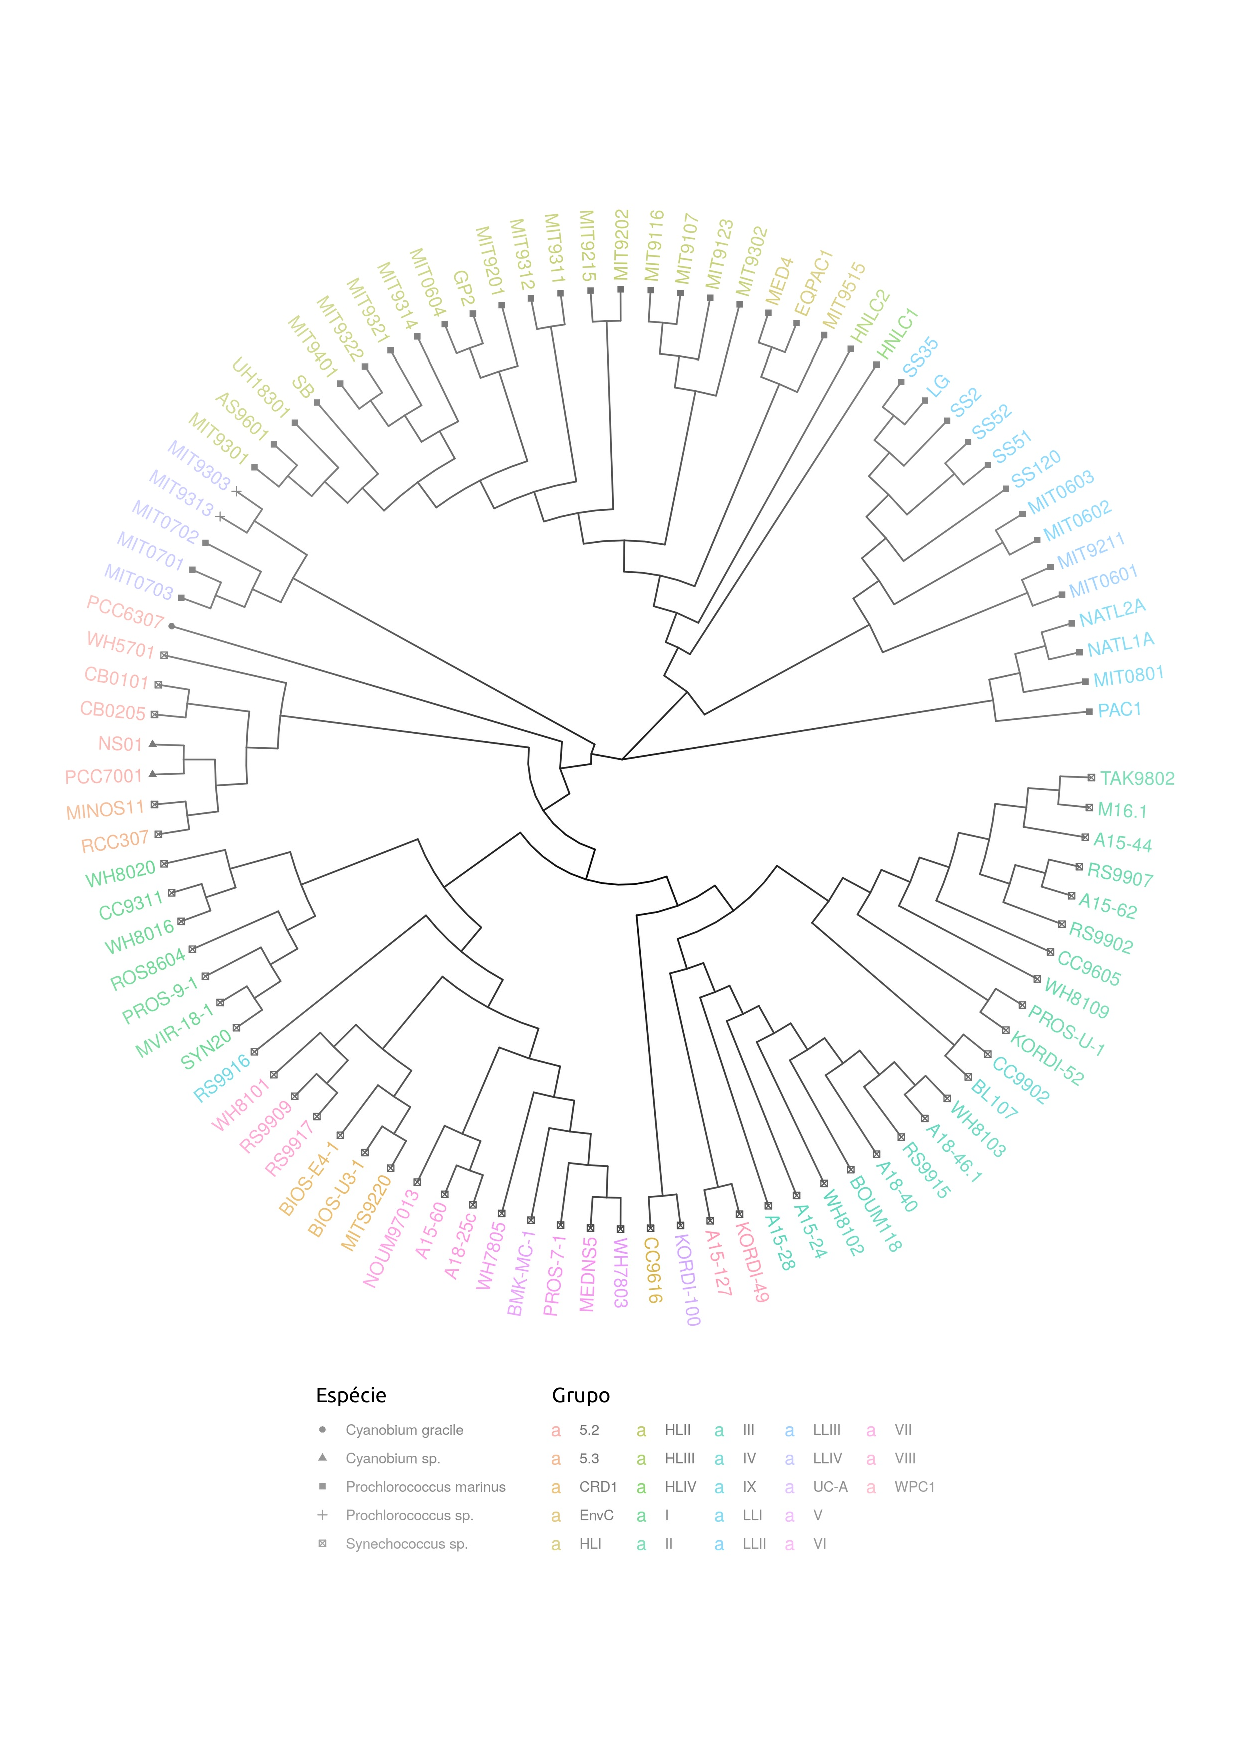
\includegraphics[width=.95\textwidth]{figures/REHDYXMS}
    \caption{Árvore filogenética baseada em rearranjos de genomas usando o Algoritmo~\ref{algorithm:MRFVALSC} com a estratégia gulosa e 97 genomas do sistema Cyanorak 2.1.} 
    \label{figure:REHDYXMS}
\end{figure}

Pela Figura~\ref{figure:REHDYXMS}, observamos que a abordagem separou os organismos considerando as espécies e realizou bons agrupamentos\footnote{Figura criada usando o pacote \texttt{treeio} da linguagem R~\cite{wang2020treeio})}. Vale ressaltar que a árvore foi baseada exclusivamente em informações de eventos de rearranjo.

\pagebreak

% % ------------------------------------------------------------------ %
\section{Abordagem Ponderada}
% % ------------------------------------------------------------------ %

Nesta seção, apresentaremos os resultados considerando diferentes funções de custo para as variações com e sem sinais dos problemas \SbWIRI{}, \SbWIRTI{} e \SbWIRT{} em um cenário ponderado.

A primeira função de custo, que chamamos de $W_1$, considera que os eventos de reversão e transposição possuem custo igual a 1, enquanto um indel tem um custo equivalente à quantidade de nucleotídeos inseridos ou removidos da região intergênica. Essa função de custo foi estudada para investigar limitantes para o modelo considerando o caso em que o peso do evento de indel é variável e está diretamente ligado com o quanto a região intergênica é afetada. A seguir, descrevemos formalmente a função de custo $W_1$:

$$
  W_1(\beta) = \begin{cases}
      |x|, \textit{para } \beta = \delta_{(x)}^{(i)} \\
      1, \textit{para } \beta = \rho_{(x,y)}^{(i,j)} \\
      1, \textit{para } \beta = \tau_{(x,y,z)}^{(i,j,k)} \\
  \end{cases}
$$

Dada uma instância intergênica rígida com ou sem sinais $\mathcal{I}=((\pi,\breve\pi),(\iota,\breve\iota))$, denotamos por $IR(\mathcal{I}) = |\sum_{\breve\pi_i \in \breve\pi} \breve\pi_i - \sum_{\breve\iota_i \in \breve\iota} \breve\iota_i|$ a quantidade de nucleotídeos que precisam ser removidos ou inseridos no genoma de origem para que $\mathcal{I}$ seja uma instância balanceada. Note que reversões e transposições podem transferir nucleotídeos entre regiões intergênicas, mas não removem ou inserem nucleotídeos. Logo, toda instância intergênica rígida com ou sem sinais $\mathcal{I}=((\pi,\breve\pi),(\iota,\breve\iota))$ para os problemas \SbWIRI{} e \SbWIRTI{} induz um custo mínimo de $IR(\mathcal{I})$, o que resulta nos seguintes limitantes inferiores.

\begin{theorem}\label{theorem:IQACALLP}
Seja $\mathcal{I} = ((\pi,\breve\pi),(\iota,\breve\iota))$ uma instância intergênica rígida sem sinais. Com base na função de custo $W_1$, temos que:

\begin{tabular}{lll}
  $dwi_{\RI}(\mathcal{I})$      & $ \ge $ & $\max(IR(\mathcal{I}),\frac{ib_1(\mathcal{I})}{2})$ e \\ 
  $dwi_{\RTI}(\mathcal{I})$     & $ \ge $ & $\max(IR(\mathcal{I}),\frac{ib_1(\mathcal{I})}{3})$.
\end{tabular}
\begin{proof}
Diretamente pelo Teorema~\ref{theorem:MPFPKHQO} e pelo custo mínimo de $IR(\mathcal{I})$ discutido anteriormente.
\end{proof}
\end{theorem}

\begin{theorem}\label{theorem:BOZETXBS}
Seja $\mathcal{I} = ((\pi,\breve\pi),(\iota,\breve\iota))$  uma instância intergênica rígida com sinais. Com base na função de custo $W_1$, temos que:

\begin{tabular}{lll}
  $dwi_{\RI}(\mathcal{I})$      & $ \ge $ & $\max(IR(\mathcal{I}),\frac{ib_2(\mathcal{I})}{2})$ e \\ 
  $dwi_{\RTI}(\mathcal{I})$     & $ \ge $ & $\max(IR(\mathcal{I}),\frac{ib_2(\mathcal{I})}{3})$.
\end{tabular}
\begin{proof}
Diretamente pelo Teorema~\ref{theorem:NFVKZGKW} e pelo custo mínimo de $IR(\mathcal{I})$ discutido anteriormente.
\end{proof}
\end{theorem}

A seguir, mostramos que, com base na função de custo $W_1$, é possível garantir aproximações para os problemas \SbWIRI{} e \SbWIRTI{} a partir de alguns dos algoritmos apresentados para o cenário não ponderado.

\begin{theorem}\label{theorem:BNWIOUVG}
O Algoritmo~\ref{algorithm:LHOPSFVN} é uma $5$-aproximação para a variação sem sinais do problema \SbWIRI{} considerando a função de custo $W_1$.
\end{theorem}
\begin{proof}
Seja $\mathcal{I} = ((\pi,\breve\pi),(\iota,\breve\iota))$ uma instância intergênica rígida sem sinais. Note que o Algoritmo~\ref{algorithm:LHOPSFVN} transforma $(\pi,\breve\pi)$ em $(\iota,\breve\iota)$ utilizando, no máximo, $2ib_1(\mathcal{I})$ eventos de reversão e indel (Lema~\ref{lemma:XUDIVWPC}). Entretanto, caso $\mathcal{I}$ seja uma instância desbalanceada, então o Algoritmo~\ref{algorithm:LHOPSFVN} aplica, no máximo, um indel com custo $IR(\mathcal{I})$. Caso contrário, apenas reversões são utilizadas. Logo, no pior caso, uma sequência de eventos de rearranjo fornecida pelo Algoritmo~\ref{algorithm:LHOPSFVN} tem um custo total de $IR(\mathcal{I}) + 2ib_1(\mathcal{I})$. Agora, consideramos duas possibilidades:
\begin{itemize}
  \item $IR(\mathcal{I}) \ge \frac{ib_1(\mathcal{I})}{2}$: Neste caso, $2IR(\mathcal{I}) \ge ib_1(\mathcal{I})$ e o custo máximo da sequência de eventos de rearranjo fornecida pelo Algoritmo~\ref{algorithm:LHOPSFVN} é $5IR(\mathcal{I})$.
  \item $IR(\mathcal{I}) < \frac{ib_1(\mathcal{I})}{2}$: Neste caso, o custo máximo da sequência de eventos de rearranjo fornecida pelo Algoritmo~\ref{algorithm:LHOPSFVN} é $\frac{5ib_1(\mathcal{I})}{2}$.
\end{itemize}
Em ambos os casos, o custo máximo da sequência de eventos de rearranjo fornecida pelo Algoritmo~\ref{algorithm:LHOPSFVN} dividido pelo valor do limitante inferior, apresentado no Teorema~\ref{theorem:IQACALLP}, é igual a $5$ e o teorema segue.
\end{proof}

\begin{theorem}\label{theorem:JKFXFCMF}
O Algoritmo~\ref{algorithm:QKCVERGO} é uma $5$-aproximação para a variação com sinais do problema \SbWIRI{} considerando a função de custo $W_1$.
\end{theorem}
\begin{proof}
A prova é similar à descrita no Teorema~\ref{theorem:BNWIOUVG}, mas considerando o Algoritmo~\ref{algorithm:QKCVERGO}, que utiliza o Algoritmo~\ref{algorithm:LHOPSFVN} em parte de sua execução, e o limitante inferior apresentado no Teorema~\ref{theorem:BOZETXBS}.
\end{proof}

\begin{theorem}\label{theorem:YATYVCZX}
O Algoritmo~\ref{algorithm:YIZYUGZZ} é uma $5$-aproximação para a variação sem sinais do problema \SbWIRTI{} considerando a função de custo $W_1$.
\end{theorem}
\begin{proof}
Seja $\mathcal{I} = ((\pi,\breve\pi),(\iota,\breve\iota))$ uma instância intergênica rígida sem sinais. Pelo Lema~\ref{lemma:MUTXDAUG}, o Algoritmo~\ref{algorithm:YIZYUGZZ} utiliza, no máximo, $\frac{4ib_1(\mathcal{I})}{3}$ ou $\frac{4ib_1(\mathcal{I})}{3} + 1$ eventos de reversão, transposição e indel para transformar $(\pi,\breve\pi)$ em $(\iota,\breve\iota)$, se $\mathcal{I}$ for balanceada ou desbalanceada, respectivamente. Entretanto, caso $\mathcal{I}$ seja uma instância desbalanceada, então Algoritmo~\ref{algorithm:YIZYUGZZ} aplica, no máximo, um indel com custo $IR(\mathcal{I})$. Caso contrário, apenas reversões e transposições são utilizadas. Logo, no pior caso, uma sequência de eventos de rearranjo fornecida pelo Algoritmo~\ref{algorithm:YIZYUGZZ} tem um custo total de $IR(\mathcal{I}) + \frac{4ib_1(\mathcal{I})}{3}$. Agora, consideramos duas possibilidades:
\begin{itemize}
  \item $IR(\mathcal{I}) \ge \frac{ib_1(\mathcal{I})}{3}$: Neste caso, $3IR(\mathcal{I}) \ge ib_1(\mathcal{I})$ e o custo máximo da sequência de eventos de rearranjo fornecida pelo Algoritmo~\ref{algorithm:YIZYUGZZ} é $IR(\mathcal{I}) + \frac{12IR(\mathcal{I})}{3} = 5IR(\mathcal{I})$.
  \item $IR(\mathcal{I}) < \frac{ib_1(\mathcal{I})}{3}$: Neste caso, o custo máximo da sequência de eventos de rearranjo fornecida pelo Algoritmo~\ref{algorithm:YIZYUGZZ} é $\frac{ib_1(\mathcal{I})}{3} + \frac{4ib_1(\mathcal{I})}{3} = \frac{5ib_1(\mathcal{I})}{3}$.
\end{itemize}
Em ambos os casos, o custo máximo da sequência de eventos de rearranjo fornecida pelo Algoritmo~\ref{algorithm:YIZYUGZZ} dividido pelo valor do limitante inferior, apresentado no Teorema~\ref{theorem:IQACALLP}, é igual a $5$ e o teorema segue.
\end{proof}

\begin{theorem}\label{theorem:XMRIBCHD}
O Algoritmo~\ref{algorithm:EQALRDVE} é uma $5$-aproximação para a variação com sinais do problema \SbWIRI{} considerando a função de custo $W_1$.
\end{theorem}
\begin{proof}
A prova é similar à descrita no Teorema~\ref{theorem:YATYVCZX}, mas considerando o Algoritmo~\ref{algorithm:EQALRDVE}, que utiliza o Algoritmo~\ref{algorithm:YIZYUGZZ} em parte de sua execução, e o limitante inferior apresentado no Teorema~\ref{theorem:BOZETXBS}.
\end{proof}

A segunda função de custo, chamada de $W_2$, é baseada no fato de que um indel afeta apenas uma região intergênica do genoma e não altera a ordem dos genes. Dessa forma, consideramos que o evento de indel possui a metade do custo de um evento de reversão ou transposição. A seguir, descrevemos formalmente a função de custo $W_2$:

$$
  W_2(\beta) = \begin{cases}
      \frac{1}{2}, \textit{para } \beta = \delta_{(x)}^{(i)} \\
      1, \textit{para } \beta = \rho_{(x,y)}^{(i,j)} \\
      1, \textit{para } \beta = \tau_{(x,y,z)}^{(i,j,k)} \\
  \end{cases}
$$

Com base nos custos da função $W_2$, obtemos para as variações com e sem sinais do problema \SbWIRTI{}, os seguintes limitantes inferiores.

\begin{theorem}\label{theorem:HFHHZDMV}
Seja $\mathcal{I} = ((\pi,\breve\pi),(\iota,\breve\iota))$ uma instância intergênica rígida sem sinais. Com base na função de custo $W_2$, temos que $dwi_{\RTI}(\mathcal{I}) \ge \frac{ib_1(\mathcal{I})}{3}$.
\begin{proof}
Pelos lemas~\ref{lemma:KFFPUBQG}, \ref{lemma:IUJZCMMV} e \ref{lemma:KWIVENLG}, sabemos que, por operação, os eventos de reversão, transposição e indel removem, respectivamente, no máximo $2$, $3$ e $1$ breakpoint tipo um. Com base no melhor caso de cada evento de rearranjo e na função de custo $W_2$, temos que:
$$dwi_{\RTI}(\mathcal{I}) \ge \min\left(\frac{ib_1(\mathcal{I})}{2} \times 1,\frac{ib_1(\mathcal{I})}{3} \times 1, ib_1(\mathcal{I}) \times \frac{1}{2}\right) = \frac{ib_1(\mathcal{I})}{3},$$ e o teorema segue.
\end{proof}
\end{theorem}

\begin{theorem}\label{theorem:IXYMBAWM}
Seja $\mathcal{I} = ((\pi,\breve\pi),(\iota,\breve\iota))$ uma instância intergênica rígida com sinais. Com base na função de custo $W_2$, temos que $dwi_{\RTI}(\mathcal{I}) \ge \frac{ib_2(\mathcal{I})}{3}$.
\begin{proof}
A prova é similar à descrita no Teorema~\ref{theorem:HFHHZDMV}, mas considerando os lemas~\ref{lemma:IKBNJWMY}, \ref{lemma:MYVALTSG} e \ref{lemma:KXIYYHHL}.
\end{proof}
\end{theorem}

\begin{lemma}\label{lemma:XLFWKWTV}
Seja $\mathcal{I}=((\pi,\breve\pi),(\iota,\breve\iota))$ uma instância intergênica rígida sem sinais e sejam $(\pi_i,\pi_{i+1})$ e $(\pi_j,\pi_{j+1})$ um par conectado de breakpoints. É possível remover pelo menos um breakpoint tipo um de $\mathcal{I}$ utilizando no máximo uma reversão, uma transposição ou dois indels.
\end{lemma}
\begin{proof}
Sem perda de generalidade, assuma que $i < j$. Como os breakpoints $(\pi_i,\pi_{i+1})$ e $(\pi_j,\pi_{j+1})$ estão conectados, por definição, uma das seguintes possibilidades deve ocorrer:
\begin{enumerate}[i.]
  \item O par de elementos $(\pi_i,\pi_{j})$ ou $(\pi_{i+1},\pi_{j+1})$ não forma uma adjacência intergênica, sendo os elementos consecutivos em $\iota$ e $\breve\pi_{i+1} + \breve\pi_{j+1} \ge \breve\iota_k$, onde $\breve\iota_k$ é o tamanho da região intergênica entre o par de elementos consecutivos em $\iota$. Aplique uma reversão como descrito no caso $(i)$ do Lema~\ref{lemma:IMYFBWDY}.
  \item O par de elementos $(\pi_i,\pi_{j+1})$ não forma uma adjacência intergênica, sendo os elementos consecutivos em $\iota$ e $\breve\pi_{i+1} + \breve\pi_{j+1} \ge \breve\iota_k$, onde $\breve\iota_k$ é o tamanho da região intergênica entre o par de elementos consecutivos em $\iota$. Aplique uma transposição como descrito no caso $(ii)$ do Lema~\ref{lemma:SIAFJFDO}.
  \item O par de elementos $(\pi_{i+1},\pi_{j})$ não forma uma adjacência intergênica, sendo os elementos consecutivos em $\iota$ e $\breve\pi_{i+1} + \breve\pi_{j+1} \ge \breve\iota_k$, onde $\breve\iota_k$ é o tamanho da região intergênica entre o par de elementos consecutivos em $\iota$. Aplique uma transposição como descrito no caso $(iii)$ do Lema~\ref{lemma:SIAFJFDO}.
  \item O par de elementos $(\pi_{i},\pi_{i+1})$ ou $(\pi_{j},\pi_{j+1})$ não forma uma adjacência intergênica, sendo os elementos consecutivos em $\iota$ e $\breve\pi_{i+1} + \breve\pi_{j+1} \ge \breve\iota_k$, onde $\breve\iota_k$ é o tamanho da região intergênica entre o par de elementos consecutivos em $\iota$. Neste caso, $(\pi_{i},\pi_{i+1})$ ou $(\pi_{j},\pi_{j+1})$ deve ser um breakpoint forte. Caso $(\pi_{i},\pi_{i+1})$ seja um breakpoint forte, então ele pode ser subcarregado ou sobrecarregado. Caso $(\pi_{i},\pi_{i+1})$ seja subcarregado, então aplique a sequência de dois indels $(\delta^{i+1}_{(x)}, \delta^{j+1}_{(-x)})$, com $x=|\breve\pi_{i+1} - \breve\iota_{\max(\pi_i, \pi_{i+1})}|$. Caso contrário, aplique a sequência de dois indels $(\delta^{i+1}_{(-x)}, \delta^{j+1}_{(x)})$, com $x=|\breve\pi_{i+1} - \breve\iota_{\max(\pi_i, \pi_{i+1})}|$. Caso $(\pi_{j},\pi_{j+1})$ seja um breakpoint forte, basta replicar a sequência de indels considerando a mudança no breakpoint. Note que essa sequência sempre pode ser aplicada, pois os dois breakpoints estão conectados. Além disso, o breakpoint tipo um é removido sem afetar quantidade total de nucleotídeos de $\mathcal{I}$.  
\end{enumerate}
Note que o caso $(i)$ aplica apenas um reversão e remove, pelo menos, um breakpoint tipo um. Os casos $(ii)$ e $(iii)$ aplicam apenas uma transposição e removem, pelo menos, um breakpoint tipo um. Por fim, o caso $(iv)$ remove, pelo menos, um breakpoint tipo um após aplicar dois indels. Logo, o lema segue.
\end{proof}

Considere o Algoritmo~\ref{algorithm:DYNWURLY} para a variação sem sinais do problema \SbWIRTI{} considerando a função de custo $W_2$.

\begin{algorithm}[!tbh]
  \caption{Um algoritmo de aproximação para o problema \SbWIRTI{}.\label{algorithm:DYNWURLY}}
  \Entrada{Uma instância intergênica rígida sem sinais $\mathcal{I}=((\pi,\breve\pi),(\iota,\breve\iota))$}
  \Saida{Uma sequência de reversões transposições e indels $S$, tal que $(\pi,\breve\pi) \cdot S = (\iota,\breve\iota)$}
    Seja $S \gets ()$ \\
    \tcp{Lema~\ref{lemma:QGOIQLZD}}
    \Se{$\sum_{i=1}^{n+1}\breve\pi_i < \sum_{i=1}^{n+1}\breve\iota_i$}{
      $S' \gets (\delta_1)$ \\
      $S \gets S + S'$ \\
      $\mathcal{I} \gets ((\pi, \breve\pi) \cdot S',(\iota,\breve\iota))$ \\
    }
    \Enqto{$ib_1(\mathcal{I}) > 1$}{
      \tcp{Lema~\ref{lemma:WYEZMYTM}}
      $(\pi_i,\pi_{i+1})$, $(\pi_j,\pi_{j+1}) \gets $ encontre um par de breakpoints conectados \\
      \tcp{Lema~\ref{lemma:XLFWKWTV}}
      \Se{$(\pi_i,\pi_{i+1})$, $(\pi_j,\pi_{j+1})$ pertence ao caso $i$}{
        $S' \gets (\rho_1)$ \\
      }\SenaoSe{$(\pi_i,\pi_{i+1})$, $(\pi_j,\pi_{j+1})$ pertence ao caso $ii$}{
        $S' \gets (\tau_1)$ \\
      }\SenaoSe{$(\pi_i,\pi_{i+1})$, $(\pi_j,\pi_{j+1})$ pertence ao caso $iii$}{
        $S' \gets (\tau_1)$ \\
      }\SenaoSe{$(\pi_i,\pi_{i+1})$, $(\pi_j,\pi_{j+1})$ pertence ao caso $iv$}{
        $S' \gets (\delta_1,\delta_2)$ \\
      }
      $S \gets S + S'$ \\
      $\mathcal{I} \gets ((\pi, \breve\pi) \cdot S',(\iota,\breve\iota))$ \\
    }
    \tcp{Lema~\ref{lemma:QNHGBLYF}}
    \Se{$ib(\mathcal{I}) = 1$}{
      $S' \gets (\delta_1)$ \\
      $S \gets S + S'$ \\
      $\mathcal{I} \gets ((\pi, \breve\pi) \cdot S',(\iota,\breve\iota))$ \\
    }
  \Retorna{S}
\end{algorithm}

\begin{lemma}\label{lemma:IKTEYDRR}
Seja $\mathcal{I} = ((\pi,\breve\pi),(\iota,\breve\iota))$ uma instância intergênica rígida sem sinais. O Algoritmo~\ref{algorithm:DYNWURLY}, considerando a função de custo $W_2$, transforma $(\pi,\breve\pi)$ em $(\iota,\breve\iota)$ utilizando uma sequência de eventos de reversão, transposição e indel $S$, com um custo total de, no máximo, $ib_1(\mathcal{I})$.
\end{lemma}
\begin{proof}
  Podemos analisar o Algoritmo~\ref{algorithm:DYNWURLY} considerando três cenários:
  \begin{itemize}
    \item $\sum_{i=1}^{n+1}\breve\pi_i < \sum_{i=1}^{n+1}\breve\iota_i$: neste cenário o Algoritmo~\ref{algorithm:DYNWURLY} aplica um indel (linhas 2-5) que pode não remover nenhum breakpoint tipo um, mas torna $\mathcal{I}$ uma instância balanceada. Caso ainda existam breakpoints em $\mathcal{I}$, então o laço de repetição (linhas 6-17) remove, por iteração, pelo menos um breakpoint tipo um utilizando, no máximo, uma reversão, uma transposição ou dois indels (Lema~\ref{lemma:XLFWKWTV}). Esse processo repete-se até que todos os breakpoints tipo um de $\mathcal{I}$ sejam removidos. Como todos os breakpoints tipo um são removidos, então $(\pi,\breve\pi)$ é transformado em $(\iota,\breve\iota)$. Note que se o indel aplicado inicialmente não remover nenhum breakpoint tipo um, então pelo menos uma reversão, uma transposição ou dois indels são aplicados em seguida. Além disso, pelo Lema~\ref{lemma:WSPRPLAH}, podemos deduzir que caso a última operação que transforma $(\pi,\breve\pi)$ em $(\iota,\breve\iota)$ seja uma reversão ou uma transposição, então ela deve, obrigatoriamente, remover pelo menos dois breakpoints tipo um. Caso essa operação seja um indel, então as duas últimas operações são indels e ambas removem um breakpoint tipo um. Isso implica que o custo total da sequência fornecida pelo Algoritmo~\ref{algorithm:DYNWURLY} é de, no máximo, $ib_1(\mathcal{I})$.
    \item $\sum_{i=1}^{n+1}\breve\pi_i = \sum_{i=1}^{n+1}\breve\iota_i$: para esse cenário o Algoritmo~\ref{algorithm:DYNWURLY} executará o laço de repetição (linhas 6-17) que remove, por iteração, pelo menos um breakpoint tipo um utilizando, no máximo, uma reversão, uma transposição ou dois indels (Lema~\ref{lemma:XLFWKWTV}). Logo, o custo total da sequência fornecida pelo Algoritmo~\ref{algorithm:DYNWURLY} é de, no máximo, $ib_1(\mathcal{I})$.
    \item $\sum_{i=1}^{n+1}\breve\pi_i > \sum_{i=1}^{n+1}\breve\iota_i$: neste último cenário, enquanto $ib_1(\mathcal{I})$ for maior que um, o Algoritmo~\ref{algorithm:DYNWURLY} aplica, no máximo, uma reversão, uma transposição ou dois indels em cada iteração do laço de repetição (linhas 6-17) que removem pelo menos um breakpoint tipo um. Por fim, um indel é aplicado (linhas 19-22) transformando $(\pi,\breve\pi)$ em $(\iota,\breve\iota)$. O custo para remover cada breakpoint nesse caso é de, no máximo, um. Logo, o custo total da sequência fornecida pelo Algoritmo~\ref{algorithm:DYNWURLY} é de, no máximo, $ib_1(\mathcal{I})$. 
  \end{itemize}
  Nos três cenários o Algoritmo~\ref{algorithm:DYNWURLY} transforma $(\pi,\breve\pi)$ em $(\iota,\breve\iota)$ utilizando uma sequência de reversões, transposições e indels com um custo total de, no máximo, $ib_1(\mathcal{I})$, e o lema segue.
\end{proof}

Note que o tempo de execução do Algoritmo~\ref{algorithm:DYNWURLY} é $\mathcal{O}(n^2)$, uma vez que aplicar cada uma das operações requer um tempo linear (considerando encontrar um par conectado de breakpoints) e o processo pode repetir-se por até $ib_1(\mathcal{I}) \le n + 1$ vezes.

\begin{theorem}\label{theorem:HXFXWAIA}
O Algoritmo~\ref{algorithm:DYNWURLY} é uma $3$-aproximação para a variação sem sinais do problema \SbWIRTI{} considerando a função de custo $W_2$.
\end{theorem}
\begin{proof}
Seja $\mathcal{I}=((\pi,\breve\pi),(\iota,\breve\iota))$ uma instância intergênica rígida sem sinais. Pelo Lema~\ref{lemma:IKTEYDRR}, o Algoritmo~\ref{algorithm:DYNWURLY} transforma $(\pi,\breve\pi)$ em $(\iota,\breve\iota)$ utilizando uma sequência de eventos de reversão, transposição e indel $S$, com um custo total de, no máximo, $ib_1(\mathcal{I})$. Pelo limitante inferior, apresentado no Teorema~\ref{theorem:HFHHZDMV}, temos que: $dwi_{\RTI}(\mathcal{I}) \ge \frac{ib_1(\mathcal{I})}{3}$. Logo, o teorema segue.
\end{proof}

Considere o Algoritmo~\ref{algorithm:HHROEWVE} para a variação com sinais do problema \SbWIRTI{} considerando a função de custo $W_2$.

\begin{algorithm}[!tbh]
  \caption{Um algoritmo de aproximação para o problema \SbWIRTI{}.\label{algorithm:HHROEWVE}}
  \Entrada{Uma instância intergênica rígida com sinais $\mathcal{I}=((\pi,\breve\pi),(\iota,\breve\iota))$}
  \Saida{Uma sequência de eventos de reversão, transposição e indel $S$, tal que $(\pi,\breve\pi) \cdot S = (\iota,\breve\iota)$}
  \tcp{Lema~\ref{lemma:FKOCCOYY}}
  $\mathcal{I'} \gets \mathcal{F}(\mathcal{I})$ \\
  Seja $S'$ uma sequência de eventos de reversão, transposição e indel fornecida pelo Algoritmo~\ref{algorithm:DYNWURLY} para a instância $\mathcal{I'}$ \\
  \tcp{Lema~\ref{lemma:GTTULLOM}}
  $S\gets \mathcal{G}(S')$ \\
  \Retorna{S}
\end{algorithm}

\begin{lemma}\label{lemma:MBYKFLMR}
Seja $\mathcal{I} = ((\pi,\breve\pi),(\iota,\breve\iota))$ uma instância intergênica rígida com sinais. O Algoritmo~\ref{algorithm:DYNWURLY}, considerando a função de custo $W_2$, transforma $(\pi,\breve\pi)$ em $(\iota,\breve\iota)$ utilizando uma sequência de eventos de reversão, transposição e indel $S$, com um custo total de, no máximo, $ib_2(\mathcal{I})$.
\end{lemma}
\begin{proof}
Note que o Algoritmo~\ref{algorithm:DYNWURLY} fornece uma sequência de reversões, transposições e indels que afetam apenas breakpoints tipo um. Logo, nenhuma adjacência intergênica de $\mathcal{I'}$ é afetada. Além disso, pelo Lema~\ref{lemma:IKTEYDRR}, o Algoritmo~\ref{algorithm:DYNWURLY} utiliza uma sequência de eventos de reversão, transposição e indel, com um custo total de, no máximo, $ib_1(\mathcal{I'})$. Pelo Lema~\ref{lemma:GTTULLOM}, temos que $(\pi,\breve\pi) \cdot S = (\iota,\breve\iota)$ e $|S| = |S'|$. Além disso, $S$ e $|S'|$ possuem a mesma quantidade de operações por tipo. Pelo Lema~\ref{lemma:FKOCCOYY}, temos que $ib_1(\mathcal{I'}) = ib_2(\mathcal{I})$. Logo, o custo total da sequência de eventos de reversão, transposição e indel fornecida pelo Algoritmo~\ref{algorithm:HHROEWVE} é de, no máximo, $ib_2(\mathcal{I})$.
\end{proof}

O Algoritmo~\ref{algorithm:HHROEWVE} também possui um tempo de execução de $\mathcal{O}(n^2)$, uma vez que as funções $\mathcal{F}$ e $\mathcal{G}$ são executadas em tempo linear e o Algoritmo~\ref{algorithm:DYNWURLY}, no pior caso, requer um tempo quadrático.

\begin{theorem}\label{theorem:MJXOZGOO}
O Algoritmo~\ref{algorithm:HHROEWVE} é uma $3$-aproximação para a variação com sinais do problema \SbWIRTI{} considerando a função de custo $W_2$.
\end{theorem}
\begin{proof}
Seja $\mathcal{I} = ((\pi,\breve\pi),(\iota,\breve\iota))$ uma instância intergênica rígida com sinais. Pelo Lema~\ref{lemma:MBYKFLMR}, o Algoritmo~\ref{algorithm:HHROEWVE} transforma $(\pi,\breve\pi)$ em $(\iota,\breve\iota)$ utilizando uma sequência de eventos de reversão, transposição e indel, com um custo total de, no máximo, $ib_2(\mathcal{I})$. Pelo limitante inferior, apresentado no Teorema~\ref{theorem:IXYMBAWM}, temos que: $dwi_{\RTI}(\mathcal{I}) \ge \frac{ib_2(\mathcal{I})}{3}$. Logo, o teorema segue.
\end{proof}

A terceira função de custo, chamada de $W_3$, é baseada na proporção de regiões intergênicas afetadas por cada evento de rearranjo~\cite{2018-alexandrino-etal}. A seguir, descrevemos formalmente a função de custo $W_3$:

$$
  W_3(\beta) = \begin{cases}
      1, \textit{para } \beta = \delta_{(x)}^{(i)} \\
      2, \textit{para } \beta = \rho_{(x,y)}^{(i,j)} \\
      3, \textit{para } \beta = \tau_{(x,y,z)}^{(i,j,k)} \\
  \end{cases}
$$

Com base nos custos da função $W_3$, obtemos para as variações com e sem sinais do problema \SbWIRTI{}, os seguintes limitantes inferiores.

\begin{theorem}\label{theorem:BFKDUKUF}
Seja $\mathcal{I} = ((\pi,\breve\pi),(\iota,\breve\iota))$ uma instância intergênica rígida sem sinais. Com base na função de custo $W_3$, temos que $dwi_{\RTI}(\mathcal{I}) \ge ib_1(\mathcal{I})$.
\begin{proof}
Pelos lemas~\ref{lemma:KFFPUBQG}, \ref{lemma:IUJZCMMV} e \ref{lemma:KWIVENLG}, sabemos que, por operação, os eventos de reversão, transposição e indel removem, respectivamente, no máximo $2$, $3$ e $1$ breakpoint tipo um. Com base no melhor caso de cada evento de rearranjo e na função de custo $W_3$, temos que:
$$dwi_{\RTI}(\mathcal{I}) \ge \min\left(\frac{ib_1(\mathcal{I})}{2} \times 2,\frac{ib_1(\mathcal{I})}{3} \times 3, ib_1(\mathcal{I}) \times 1\right) = ib_1(\mathcal{I}),$$ e o teorema segue.
\end{proof}
\end{theorem}

\begin{theorem}\label{theorem:ACJPZCWD}
Seja $\mathcal{I} = ((\pi,\breve\pi),(\iota,\breve\iota))$ uma instância intergênica rígida com sinais. Com base na função de custo $W_3$, temos que $dwi_{\RTI}(\mathcal{I}) \ge ib_2(\mathcal{I})$.
\begin{proof}
A prova é similar à descrita no Teorema~\ref{theorem:BFKDUKUF}, mas considerando os lemas~\ref{lemma:IKBNJWMY}, \ref{lemma:MYVALTSG} e \ref{lemma:KXIYYHHL}.
\end{proof}
\end{theorem}

\begin{lemma}\label{lemma:FESYSSFB}
Seja $\mathcal{I} = ((\pi,\breve\pi),(\iota,\breve\iota))$ uma instância intergênica rígida sem sinais. o Algoritmo~\ref{algorithm:DYNWURLY}, considerando a função de custo $W_3$, transforma $(\pi,\breve\pi)$ em $(\iota,\breve\iota)$ utilizando uma sequência de eventos de reversão, transposição e indel $S$, com um custo total de, no máximo, $3ib_1(\mathcal{I})$.
\end{lemma}
\begin{proof}
  A prova é similar à descrita no Lema~\ref{lemma:IKTEYDRR} considerando a função de custo $W_3$.
\end{proof}

\begin{theorem}\label{theorem:YFYDIUAB}
O Algoritmo~\ref{algorithm:DYNWURLY} é uma $3$-aproximação para a variação sem sinais do problema \SbWIRTI{} considerando a função de custo $W_3$.
\end{theorem}
\begin{proof}
Seja $\mathcal{I} = ((\pi,\breve\pi),(\iota,\breve\iota))$ uma instância intergênica rígida sem sinais. Pelo Lema~\ref{lemma:FESYSSFB}, o Algoritmo~\ref{algorithm:DYNWURLY} transforma $(\pi,\breve\pi)$ em $(\iota,\breve\iota)$ utilizando uma sequência de eventos de reversão, transposição e indel $S$, com um custo total de, no máximo, $3ib_1(\mathcal{I})$. Pelo limitante inferior, apresentado no Teorema~\ref{theorem:BFKDUKUF}, temos que: $dwi_{\RTI}(\mathcal{I}) \ge ib_1(\mathcal{I})$. Logo, o teorema segue.
\end{proof}

\begin{lemma}\label{lemma:HRFGEWNU}
Seja $\mathcal{I} = ((\pi,\breve\pi),(\iota,\breve\iota))$ uma instância intergênica rígida com sinais. O Algoritmo~\ref{algorithm:HHROEWVE}, considerando a função de custo $W_3$, transforma $(\pi,\breve\pi)$ em $(\iota,\breve\iota)$ utilizando uma sequência de eventos de reversão, transposição e indel $S$, com um custo total de, no máximo, $3ib_2(\mathcal{I})$.
\end{lemma}
\begin{proof}
  A prova é similar à descrita no Lema~\ref{lemma:MBYKFLMR} considerando a função de custo $W_3$.
\end{proof}

\begin{theorem}\label{theorem:UMSMTVTN}
O Algoritmo~\ref{algorithm:HHROEWVE} é uma $3$-aproximação para a variação com sinais do problema \SbWIRTI{} considerando a função de custo $W_3$.
\end{theorem}
\begin{proof}
Pelo Lema~\ref{lemma:HRFGEWNU}, o Algoritmo~\ref{algorithm:HHROEWVE} transforma $(\pi,\breve\pi)$ em $(\iota,\breve\iota)$ utilizando uma sequência de eventos de reversão, transposição e indel $S$, com um custo total de, no máximo, $3ib_2(\mathcal{I})$. Pelo limitante inferior, apresentado no Teorema~\ref{theorem:ACJPZCWD}, temos que: $dwi_{\RTI}(\mathcal{I}) \ge ib_2(\mathcal{I})$. Logo, o teorema segue.
\end{proof}

A seguir, apresentamos duas funções de custo para o problema \SbWIRT{} que são amplamente utilizadas na literatura em modelos compostos pelos eventos conservativos de reversão e transposição. A primeira função de custo, chamada de $W_4$, adota os custos $1$ e $2$ para os eventos de reversão e transposição, respectivamente~\cite{2002-eriksen}. A segunda função de custo, chamada de $W_5$, adota os custos $2$ e $3$ para os eventos de reversão e transposição, respectivamente~\cite{2019a-oliveira-etal}. A seguir, descrevemos formalmente as funções de custo $W_4$ e $W_5$:

$$
  W_4(\beta) = \begin{cases}
      1, \textit{para } \beta = \rho_{(x,y)}^{(i,j)} \\
      2, \textit{para } \beta = \tau_{(x,y,z)}^{(i,j,k)} \\
  \end{cases}
$$ 

$$
  W_5(\beta) = \begin{cases}
      2, \textit{para } \beta = \rho_{(x,y)}^{(i,j)} \\
      3, \textit{para } \beta = \tau_{(x,y,z)}^{(i,j,k)} \\
  \end{cases}
$$

Com base nos custos da funções $W_4$, obtemos para as variações com e sem sinais do problema \SbWIRT{}, os seguintes limitantes inferiores.

\begin{theorem}\label{theorem:TUSWAWTT}
Seja $\mathcal{I} = ((\pi,\breve\pi),(\iota,\breve\iota))$ uma instância intergênica rígida balanceada sem sinais. Com base na função de custo $W_4$, temos que $dwi_{\RT}(\mathcal{I}) \ge \frac{ib_1(\mathcal{I})}{2}$.
\begin{proof}
Pelos lemas~\ref{lemma:KFFPUBQG}, \ref{lemma:IUJZCMMV}, sabemos que, por operação, os eventos de reversão e transposição removem, respectivamente, no máximo, $2$ e $3$ breakpoints tipo um. Com base no melhor caso de cada evento de rearranjo e na função de custo $W_4$, temos que:
$$dwi_{\RT}(\mathcal{I}) \ge \min\left(\frac{ib_1(\mathcal{I})}{2} \times 1,\frac{ib_1(\mathcal{I})}{3} \times 2\right) = \frac{ib_1(\mathcal{I})}{2},$$ e o teorema segue.
\end{proof}
\end{theorem}

\begin{theorem}\label{theorem:RPTOVHAP}
Seja $\mathcal{I} = ((\pi,\breve\pi),(\iota,\breve\iota))$ uma instância intergênica rígida balanceada com sinais. Com base na função de custo $W_4$, temos que $dwi_{\RT}(\mathcal{I}) \ge \frac{ib_2(\mathcal{I})}{2}$.
\begin{proof}
A prova é similar à descrita no Teorema~\ref{theorem:TUSWAWTT}, mas considerando os lemas~\ref{lemma:IKBNJWMY} e \ref{lemma:MYVALTSG}.
\end{proof}
\end{theorem}

\begin{lemma}\label{lemma:DDSJVECJ}
Seja $\mathcal{I}=((\pi,\breve\pi),(\iota,\breve\iota))$ uma instância intergênica rígida balanceada sem sinais. O Algoritmo~\ref{algorithm:JQHVZACM}, considerando a função de custo $W_4$, transforma $(\pi,\breve\pi)$ em $(\iota,\breve\iota)$ utilizando uma sequência de eventos de reversão e transposição $S$, com um custo total de, no máximo, $2ib_1(\mathcal{I})$.
\end{lemma}
\begin{proof}
Pelo Lema~\ref{lemma:RNJHXOWZ}, sabemos que o Algoritmo~\ref{algorithm:JQHVZACM} transforma $(\pi,\breve\pi)$ em $(\iota,\breve\iota)$. Para obtermos o custo total máximo de uma sequência de reversões e transposições fornecida pelo Algoritmo~\ref{algorithm:JQHVZACM} vamos considerar suas duas fases: (i) remoção de breakpoints sobrecarregados: nessa fase cada breakpoint tipo um é removido com um custo médio de $2$, no pior caso; (ii) remoção de breakpoints suaves: no pior caso, cada breakpoint tipo um é removido por uma transposição, que tem custo $2$. Dessa forma, o custo total máximo de uma sequência de reversões e transposições fornecida pelo Algoritmo~\ref{algorithm:JQHVZACM} é $2ib_1(\mathcal{I})$, e o lema segue. 
\end{proof}

\begin{theorem}\label{theorem:CQXBDUDY}
O Algoritmo~\ref{algorithm:JQHVZACM} é uma $4$-aproximação para a variação sem sinais do problema \SbWIRT{} considerando a função de custo $W_4$.
\end{theorem}
\begin{proof}
Seja $\mathcal{I} = ((\pi,\breve\pi),(\iota,\breve\iota))$ uma instância intergênica rígida balanceada sem sinais. Pelo Lema~\ref{lemma:DDSJVECJ}, o Algoritmo~\ref{algorithm:JQHVZACM}, com base na função de custo $W_4$, transforma $(\pi,\breve\pi)$ em $(\iota,\breve\iota)$ utilizando uma sequência de eventos de reversão e transposição com um custo total de, no máximo, $2ib_1(\mathcal{I})$. Pelo limitante inferior, apresentado no Teorema~\ref{theorem:TUSWAWTT}, temos que: $dwi_{\RT}(\mathcal{I}) \ge \frac{ib_2(\mathcal{I})}{2}$. Logo, o teorema segue.
\end{proof}

Considere o Algoritmo~\ref{algorithm:JRRYCBXN} para a variação com sinais do problema \SbWIRT{} considerando a função de custo $W_4$.

\begin{algorithm}[!tbh]
  \caption{Um algoritmo de aproximação para o problema \SbWIRT{}.\label{algorithm:JRRYCBXN}}
  \Entrada{Uma instância intergênica rígida com sinais $\mathcal{I}=((\pi,\breve\pi),(\iota,\breve\iota))$}
  \Saida{Uma sequência de eventos de reversão e transposição $S$, tal que $(\pi,\breve\pi) \cdot S = (\iota,\breve\iota)$}
  \tcp{Lema~\ref{lemma:FKOCCOYY}}
  $\mathcal{I'} \gets \mathcal{F}(\mathcal{I})$ \\
  Seja $S'$ uma sequência de eventos de reversão e transposição fornecida pelo Algoritmo~\ref{algorithm:JQHVZACM} \\
  \tcp{Lema~\ref{lemma:GTTULLOM}}
  $S\gets \mathcal{G}(S')$ \\
  \Retorna{S}
\end{algorithm}

\begin{lemma}\label{lemma:TMZVZPOF}
Seja $\mathcal{I} = ((\pi,\breve\pi),(\iota,\breve\iota))$ uma instância intergênica rígida balanceada com sinais. O Algoritmo~\ref{algorithm:JRRYCBXN}, considerando a função de custo $W_4$, transforma $(\pi,\breve\pi)$ em $(\iota,\breve\iota)$ utilizando uma sequência de eventos de reversão e transposição $S$, com um custo total de, no máximo, $2ib_2(\mathcal{I})$.
\end{lemma}
\begin{proof}
Note que o Algoritmo~\ref{algorithm:JQHVZACM} fornece uma sequência de reversões e transposições que afetam apenas breakpoints tipo um. Logo, nenhuma adjacência intergênica de $\mathcal{I'}$ é afetada. Além disso, pelo Lema~\ref{lemma:DDSJVECJ}, o Algoritmo~\ref{algorithm:JQHVZACM} utiliza uma sequência de eventos de reversão e transposição com um custo total de, no máximo, $2ib_1(\mathcal{I'})$ para transformar $(\pi',\breve\pi')$ em $(\iota',\breve\iota')$. Pelo Lema~\ref{lemma:GTTULLOM}, temos que $(\pi,\breve\pi) \cdot S = (\iota,\breve\iota)$ e $|S| = |S'|$. Além disso, $S$ e $|S'|$ possuem a mesma quantidade de operações por tipo. Pelo Lema~\ref{lemma:FKOCCOYY}, temos que $2ib_1(\mathcal{I'}) = 2ib_2(\mathcal{I})$. Logo, o custo total da sequência de eventos de reversão e transposição fornecida pelo Algoritmo~\ref{algorithm:JRRYCBXN} é de, no máximo, $2ib_2(\mathcal{I})$.
\end{proof}

\begin{theorem}\label{theorem:IUDGQWGI}
O Algoritmo~\ref{algorithm:JRRYCBXN} é uma $4$-aproximação para a variação com sinais do problema \SbWIRT{} considerando a função de custo $W_4$.
\end{theorem}
\begin{proof}
Seja $\mathcal{I} = ((\pi,\breve\pi),(\iota,\breve\iota))$ uma instância intergênica rígida balanceada com sinais. Pelo Lema~\ref{lemma:TMZVZPOF}, o Algoritmo~\ref{algorithm:JRRYCBXN}, com base na função de custo $W_4$, transforma $(\pi,\breve\pi)$ em $(\iota,\breve\iota)$ utilizando uma sequência de eventos de reversão e transposição com um custo total de, no máximo, $2ib_2(\mathcal{I})$. Pelo limitante inferior, apresentado no Teorema~\ref{theorem:RPTOVHAP}, temos que $dwi_{\RT}(\mathcal{I}) \ge \frac{ib_2(\mathcal{I})}{2}$. Logo, o teorema segue.
\end{proof}

Com base nos custos da funções $W_5$, obtemos para as variações com e sem sinais do problema \SbWIRT{}, os seguintes limitantes inferiores.

\begin{theorem}\label{theorem:XDQCRTEI}
Seja $\mathcal{I} = ((\pi,\breve\pi),(\iota,\breve\iota))$ uma instância intergênica rígida balanceada sem sinais. Com base na função de custo $W_5$, temos que $dwi_{\RT}(\mathcal{I}) \ge ib_1(\mathcal{I})$.
\begin{proof}
Pelos lemas~\ref{lemma:KFFPUBQG} e \ref{lemma:IUJZCMMV}, sabemos que, por operação, os eventos de reversão e transposição removem, respectivamente, no máximo $2$e $3$ breakpoints tipo um. Com base no melhor caso de cada evento de rearranjo e na função de custo $W_5$, temos que:
$$dwi_{\RT}(\mathcal{I}) \ge \min\left(\frac{ib_1(\mathcal{I})}{2} \times 2,\frac{ib_1(\mathcal{I})}{3} \times 3\right) = ib_1(\mathcal{I}),$$ e o teorema segue.
\end{proof}
\end{theorem}

\begin{theorem}\label{theorem:MCKFPIOP}
Seja $\mathcal{I} = ((\pi,\breve\pi),(\iota,\breve\iota))$ uma instância intergênica rígida balanceada com sinais. Com base na função de custo $W_5$, temos que $dwi_{\RT}(\mathcal{I}) \ge ib_2(\mathcal{I})$.
\begin{proof}
A prova é similar à descrita no Teorema~\ref{theorem:XDQCRTEI}, mas considerando os lemas~\ref{lemma:IKBNJWMY} e \ref{lemma:MYVALTSG}.
\end{proof}
\end{theorem}

\begin{lemma}\label{lemma:ODPHCEIG}
Seja $\mathcal{I} = ((\pi,\breve\pi),(\iota,\breve\iota))$ uma instância intergênica rígida balanceada sem sinais. O Algoritmo~\ref{algorithm:JQHVZACM}, considerando a função de custo $W_5$, transforma $(\pi,\breve\pi)$ em $(\iota,\breve\iota)$ utilizando uma sequência de eventos de reversão e transposição $S$, com um custo total de, no máximo, $\frac{7ib_1(\mathcal{I})}{2}$.
\end{lemma}
\begin{proof}
Pelo Lema~\ref{lemma:RNJHXOWZ}, sabemos que o Algoritmo~\ref{algorithm:JQHVZACM} transforma $(\pi,\breve\pi)$ em $(\iota,\breve\iota)$. Para obtermos o custo total máximo de uma sequência de reversões e transposições fornecida pelo Algoritmo~\ref{algorithm:JQHVZACM} vamos considerar suas duas fases: (i) remoção de breakpoints sobrecarregados: nessa fase cada breakpoint tipo um é removido com um custo médio de $4$, no pior caso; (ii) remoção de breakpoints suaves: no pior caso, cada breakpoint tipo um é removido por uma transposição, que tem custo $3$. Entretanto, se ocorrer o pior caso da fase de remoção de breakpoints sobrecarregados, então a fase de remoção de breakpoints suaves será executada em seguida. Dessa forma, no pior caso, dois breakpoints tipo um são removidos com um custo de $4 + 3 = 7$. Logo, o custo total máximo de uma sequência de reversões e transposições fornecida pelo Algoritmo~\ref{algorithm:JQHVZACM} é $\frac{ib_1(\mathcal{I})}{2} \times 7 = \frac{7ib_1(\mathcal{I})}{2}$, e o lema segue. 
\end{proof}

\begin{theorem}\label{theorem:SEJEYSUH}
O Algoritmo~\ref{algorithm:JQHVZACM} é uma $3.5$-aproxima\-ção para a variação sem sinais do problema \SbWIRT{} considerando a função de custo $W_5$.
\end{theorem}
\begin{proof}
Seja $\mathcal{I} = ((\pi,\breve\pi),(\iota,\breve\iota))$ uma instância intergênica rígida balanceada sem sinais. Pelo Lema~\ref{lemma:ODPHCEIG}, o Algoritmo~\ref{algorithm:JQHVZACM}, com base na função de custo $W_5$, transforma $(\pi,\breve\pi)$ em $(\iota,\breve\iota)$ utilizando uma sequência de eventos de reversão e transposição com um custo total de, no máximo, $\frac{7ib_1(\mathcal{I})}{2}$. Pelo limitante inferior, apresentado no Teorema~\ref{theorem:XDQCRTEI}, temos que: $dwi_{\RT}(\mathcal{I}) \ge ib_1(\mathcal{I})$. Logo, o teorema segue.
\end{proof}

\begin{lemma}\label{lemma:MUTSEXQW}
Seja $\mathcal{I} = ((\pi,\breve\pi),(\iota,\breve\iota))$ uma instância intergênica rígida balanceada com sinais. O Algoritmo~\ref{algorithm:JRRYCBXN},  considerando a função de custo $W_5$, transforma $(\pi,\breve\pi)$ em $(\iota,\breve\iota)$ utilizando uma sequência de eventos de reversão e transposição $S$, com um custo total de, no máximo, $\frac{7ib_2(\mathcal{I})}{2}$.
\end{lemma}
\begin{proof}
A prova é similar à descrita no Lema~\ref{lemma:TMZVZPOF} considerando a função de custo $W_5$.
\end{proof}

\begin{theorem}\label{theorem:ZYFESTTM}
O Algoritmo~\ref{algorithm:JRRYCBXN} é uma $3.5$-aproxima\-ção para a variação com sinais do problema \SbWIRT{} considerando a função de custo $W_5$.
\end{theorem}
\begin{proof}
Seja $\mathcal{I} = ((\pi,\breve\pi),(\iota,\breve\iota))$ uma instância intergênica rígida balanceada com sinais. Pelo Lema~\ref{lemma:MUTSEXQW}, o Algoritmo~\ref{algorithm:JQHVZACM}, com base na função de custo $W_5$, transforma $(\pi,\breve\pi)$ em $(\iota,\breve\iota)$ utilizando uma sequência de eventos de reversão e transposição com um custo total de, no máximo, $\frac{7ib_2(\mathcal{I})}{2}$. Pelo limitante inferior, apresentado no Teorema~\ref{theorem:MCKFPIOP}, temos que: $dwi_{\RT}(\mathcal{I}) \ge ib_2(\mathcal{I})$. Logo, o teorema segue.
\end{proof}


% % ------------------------------------------------------------------ %
\section{Conclusões}
% % ------------------------------------------------------------------ %

Neste capítulo, investigamos as variações com e sem sinais de oito problemas considerando instâncias intergênicas rígidas em um cenário não ponderado e os eventos de rearranjo de reversão, transposição, move e indel. Para todas as variações dos problemas em que a complexidade ainda era desconhecida, apresentamos uma prova de NP-dificuldade, com exceção da variação com sinais do problema de Ordenação de Permutações por Operações Intergênicas de Reversão e Indel (\SbIRI). Para todas as variações investigadas, apresentamos pelo menos um algoritmo de aproximação com fator constante baseado no conceito de breakpoint intergênico. Além disso, apresentamos algoritmos com fatores de aproximação melhores baseados na estrutura de grafo de ciclos ponderado rígido.

Realizamos testes experimentais com os algoritmos propostos para verificar o desempenho prático dos mesmos. Além disso, utilizamos dados de 97 genomas reais e construímos uma árvore filogenética com base exclusivamente na matriz de distâncias fornecida por um dos nossos algoritmos. Comparamos essa árvore filogenética com outra presente na literatura, construída com os mesmos 97 genomas, e o resultado apontou que existe uma alta concordância entre elas.

Em um cenário ponderado, investigamos as variações com e sem sinais de três problemas considerando instâncias intergênicas rígidas e os eventos de rearranjo de reversão, transposição e indel. Consideramos diferentes funções de custo e apresentamos algoritmos de aproximação com um fator constante para todas as variações investigadas.